% Vorlage für Abschlussarbeiten
%
% arbeit.tex
%
% Das ist das zentrale Dokument.

% allgemeine Einstellungen
% Vorlage für Abschlussarbeiten
%
% einstellungen.tex
%
% Hier werden allgemeine Einstellungen festgelegt.

\documentclass[%
	a4paper,%							A4 Papier
	oneside,%							einseitig (linker und rechter Seitenrand sind gleich groß)
	bibliography=totoc,%	Literaturverzeichnis nummeriert mit ins Inhaltsverzeichnis einfügen
	listof=totoc,%				Abbildungs- und Tabellenverzeichnis ins Inhaltsverzeichnis einfügen
	numbers=noenddot,%		hinter der Gliederungsnummer soll kein Punkt gesetzt werden (siehe Duden)
	parskip=false,%				europäischer Satz mit Abstand zwischen Absätzen
	headsepline,%					Linie nach Kopfzeile
	captions=tableheading,%		Tabellenueberschriften mit passendem Abstand setzen
	headheight=17pt,%
	chapterprefix=false,%	kein "Kapitel N" über der Kapitelüberschrift
	11pt,%								11 pt Grundschrift (Leitfäden: 11–12 pt), mit \onehalfspacing 16,5 pt Zeilenabstand = Word 1,3
]{scrreprt}

% Laut Duden gilt:
% Bei rein arabischer Nummerierung soll der Punkt
% weggelassen werden. Werden auch römische Zahlen und
% Buchstaben für die Gliederung verwendet, soll ein
% abschließender Punkt gesetzt werden. Als Voreinstellung
% versucht KOMA-Script, dies automatisch herauszufinden. (Da
% es sich diese Information in der .aux-Datei merkt, kann ein
% weiterer LATEX-Lauf notwendig sein.)
% Paket für Deutsche Sprache (Übersetzungen von Chapter zu Kapitel, 
% richtige Umlaute, richtige % Silbentrennung)
% siehe auch http://de.wikipedia.org/wiki/Babel-System
\usepackage[english,ngerman]{babel}

% Eingabecodierung, deutsche Umlaute oder die akzentuierten Zeichen sind verfügbar 
% und können direkt eingegeben werden
% siehe auch http://de.wikipedia.org/wiki/UTF8
\usepackage[utf8]{inputenc}

% Ausgabeschriftart von LaTeX festlegen
% siehe auch http://de.wikibooks.org/wiki/LaTeX-Schnellkurs:_Erste_Schritte
\usepackage[T2A,T1]{fontenc}
\DeclareUnicodeCharacter{0403}{{\fontencoding{T2A}\fontfamily{cmr}\selectfont\CYRGUP}}
\DeclareUnicodeCharacter{043D}{{\fontencoding{T2A}\fontfamily{cmr}\selectfont\cyrn}}

% schönere Schriftart
\renewcommand*{\ttdefault}{lmtt}
\usepackage{newpxtext}

% mikrotypografische Verbesserungen
\usepackage{microtype}
\microtypesetup{protrusion=true,expansion=true}
\DeclareMicrotypeSet{thesistext}{encoding={T1,TS1}}
\UseMicrotypeSet[expansion]{thesistext}

% Paket zum Erweitern der Tabelleneigenschaften
\usepackage{array}
\usepackage{longtable}

% Paket zum Überprüfen, ob ein pdf oder etwas anderes erstellt wird
\usepackage{ifpdf}

% Paket um Grafiken einbetten zu können
% erlaubt sind die Formate png, pdf, jpg
% nicht erlaubt sind eps/ps für pdftex/pdflatex
\usepackage{graphicx}
\usepackage{float}
% Standardpfad für Grafiken
\graphicspath{{bilder/}}
% Standardendung für Grafiken
\ifpdf
	% für die pdf-Ausgabe
	\DeclareGraphicsExtensions{.pdf,.jpg,.png}
\else
	% für die html-Ausgabe
	\DeclareGraphicsExtensions{.png,.jpg}
\fi

% ermöglicht Punkte in Dateinamen von Bildern
\usepackage{grffile}

\usepackage{xcolor}

% Paket zum "Zeichnen" von Grafiken (TikZ ist kein Zeichenprogramm)
\usepackage{tikz}
\usetikzlibrary{positioning,arrows.meta,fit,calc,shapes.misc,shapes.geometric}

% Paket zum Zeichnen von elektrischen Schaltkreisen mit TikZ
\usepackage[european,EFvoltages]{circuitikz}
\def\TikZ{Ti\emph{k}Z}
\def\Circuitikz{Circui\TikZ}

% Paket zum Erstellen von Plots mit TikZ
\usepackage{pgfplots}
% immer die neueste Version benutzen
\pgfplotsset{compat=newest}
% Verbindung von Linien durch eine schräge Kante
\pgfplotsset{every axis/.append style={line join=bevel}}
% neue Größenvorlage für zwei Plots nebeneinander anlegen
\pgfplotsset{
	scriptsize/.style={
		width=4.5cm,
		height=,
		legend style={font=\scriptsize},
		tick label style={font=\scriptsize},
		label style={font=\footnotesize},
		title style={font=\footnotesize},
		every axis title shift=0pt,
		max space between ticks=15,
		every mark/.append style={mark size=7},
		major tick length=0.1cm,
		minor tick length=0.066cm,
	},
}
% Legendeneintrage standardmäßig links ausrichten
\pgfplotsset{legend cell align=left}
% Anzahl der kleinen Teilstriche zwischen zwei großen Teilstrichen
%\pgfplotsset{minor x tick num={3}}
%\pgfplotsset{minor y tick num={3}}
% feines Gitternetz zeichnen
%\pgfplotsset{xminorgrids}
%\pgfplotsset{yminorgrids}
% nur nach den Achsen skalieren
\pgfplotsset{scale only axis}
% Farben wie in MATLAB definieren (Version R2014a und früher)
%%%%%%%% Farben wie in MATLAB definieren (ab Version R2014b)
% siehe: https://de.mathworks.com/help/matlab/graphics_transition/why-are-plot-lines-different-colors.html
% Die RGB-Werte können auch per
% >> figure;
% >> get(gca,'defaultAxesColorOrder');
% ausgelesen werden.
% Vielen Dank an Thomas Aab für die Aktualisierung.
% Farbreihenfolge von pgfplots benutzen
%\pgfplotsset{cycle list name=color list}
% nur Graustufen benutzen
%\pgfplotsset{cycle list name=linestyles}
% Strichstärke auf 1pt festlegen
\pgfplotsset{every axis plot/.append style={line width=1pt}}
% für deutsche Dokumente ein Komma benutzen
\addto\extrasngerman{\pgfplotsset{/pgf/number format/.cd,set decimal separator={{{,}}}}}
% ein halbes Leerzeichen als Tausendertrennzeichen benutzen
\pgfplotsset{/pgf/number format/.cd,1000 sep={\,}}

% Paket um mehrere Grafiken als eine Abbildung darstellen zu können
\usepackage{subfig}

% mathematische Symbole aus dem AMS (Amerikanische Mathematische Gesellschaft) Paket
\usepackage{amsmath}
\numberwithin{equation}{chapter}
% links-ausgerichtete Gleichungen
%\usepackage[fleqn]{amsmath}
\usepackage{newpxmath}
\usepackage{bm}
% kein zusätzlicher Abstand nach dem Dezimalkomma im Mathemodus
\usepackage{icomma}

% Paket um den Zeilenabstand zu ändern
\usepackage{setspace}
% Zeilenabstand 1,1 (wie die THB-LaTeX-Vorlage)
%\setstretch{1.1}
\onehalfspacing
\emergencystretch=2em
\clubpenalty=10000
\widowpenalty=10000
\displaywidowpenalty=10000

% Paket um Textteile drehen zu können
\usepackage{rotating}

% Paket für bessere Tabellen
\usepackage{booktabs}


% Seitenstil und Typografie werden in gestaltung.tex konfiguriert.
\usepackage[automark]{scrlayer-scrpage}

% Package für die deutsche BibTeX-Umgebung
% (sonst kann man keine Auflage eines Buches angeben)
\usepackage[backend=biber,style=numeric-comp,sorting=none,maxbibnames=99,maxcitenames=2,giveninits=true,
  uniquename=init,doi=true,isbn=false,url=true,eprint=true,date=year,urldate=long,urldateusetime=true,urltime=24h]{biblatex}

\DefineBibliographyStrings{ngerman}{
	andothers = {{et\addabbrvspace al\adddot}},
	urlfrom = {{Verfügbar unter}},
	urlseen = {Zugriff am},
}

% Datum und Uhrzeit des Abrufs mit Komma trennen (Leitfaden 4.5.3)
\DefineBibliographyExtras{ngerman}{\renewcommand*{\bibdatetimesep}{\addcomma\space}}

\DeclareFieldFormat*{url}{\bibstring{urlfrom}\addcolon\space\url{#1}}

\addbibresource{literatur.bib}  % Name deiner .bib-Datei anpassen
% Paket für bessere Anführungszeichen
\usepackage{csquotes}

% Paket für bessere Zitate


% Paket, um zu Verhindern, dass Zitate im Inhaltsverzeichnis, Abbildungsverzeichnis und Tabellenverzeichnis die Nummerierung beeinflussen
\usepackage{notoccite}

% Paket für Unterstreichungen
\usepackage[normalem]{ulem}

% Paket zur Änderung von Aufzählungen
\usepackage{enumitem}

% neue Umgebung für eine Aufzählung (unnummeriert) mit weniger vertikalen Abständen
\newenvironment{packed_itemize}{
\begin{itemize}[topsep=0pt,partopsep=0pt]
	\setlength{\itemsep}{0pt}
	\setlength{\parskip}{0pt}
	\setlength{\parsep}{0pt}
}{\end{itemize}}

% neue Umgebung für eine Aufzählung (nummeriert) mit weniger vertikalen Abständen
\newenvironment{packed_enumerate}{
\begin{enumerate}[topsep=0pt,partopsep=0pt]
	\setlength{\itemsep}{0pt}
	\setlength{\parskip}{0pt}
	\setlength{\parsep}{0pt}
}{\end{enumerate}}

% Paket für SI-Einheiten
\usepackage{siunitx}
% Optionen für das Paket
% Einstellungen in gestaltung.tex




% Paket zur Darstellung von Algorithmen
%\usepackage{algorithm2e}

% Paket für ein intelligenter Leerzeichen
\usepackage{xspace}

% ein paar Befehle für häufig benutzte Abkürzungen

% Markierung für Angaben, die der Verfasser noch bestätigen oder ergänzen muss
\newcommand{\pruefen}[1]{\textcolor{red!75!black}{[prüfen: #1]}}
\newcommand{\zB}{z.\,B.\xspace}
\newcommand{\dH}{d.\,h.\xspace} % den /dh-Befehl gibt es schon
% Kürzel der supervised Referenz (ÜBl. = überwachte Baseline). Nur hier ändern.
% Der Punkt entfällt, wenn im Text schon ein Punkt folgt (\UEBL. am Satzende ergibt ÜBl.).
\makeatletter
\DeclareRobustCommand{\UEBL}{ÜBl\@ifnextchar.{}{.\xspace}}
\makeatother

% neue mathematische Funktionen definieren
\DeclareMathOperator{\arcosh}{arcosh}
\DeclareMathOperator*{\argmax}{arg\,max}
\DeclareMathOperator*{\argmin}{arg\,min}

% Differentialoperator (kleines aufrechtes d)
\newcommand*{\diff}{\mathop{}\!\mathrm{d}}

% e-Funktion umdefinieren
\newcommand{\e}{\mathrm{e}}

% Indizes aufrecht (in Roman) schreiben
\newcommand{\ind}[1]{\mathrm{#1}}

% Punkt in einer Formelumgebung, z.B. am Ende einer Formel
\newcommand{\punkt}{\,\text{.}}
% ebenso Komma
\newcommand{\komma}{\,\text{,}}

% Betrag oder Absolutwert
\newcommand{\abs}[1]{\left| #1 \right|}

% Mittelwert oder Durchschnitt
\newcommand{\mean}[1]{\left\langle #1 \right\rangle}

% Paket für schönere Brüche im Textmodus
\usepackage{xfrac}
% Standardeinstellung wie im herkömmlichen Mathemodus mit schrägen Virgule-Bruchstrich
%\UseCollection{xfrac}{plainmath}

% Seitenränder: 3 cm auf allen Seiten (Kopfzeile liegt im oberen Rand, Seitenzahl der Kapitelanfänge im unteren)
\usepackage[margin=30mm,headheight=17pt,headsep=8mm,footskip=12mm]{geometry}
\raggedbottom

% bestimmte Trennung für bestimmte Wörter
\hyphenation{Mi-kro-strei-fen-lei-ters ver-schie-den-klas-si-ge ver-schie-den-klas-si-gen Me-cha-nis-mus}

% Paket für ein Symbolverzeichnis/Notationsverzeichnis
\usepackage[german]{nomencl}
\makenomenclature

% Paket für ein Abkürzungsverzeichnis
% - siehe http://de.wikibooks.org/wiki/LaTeX-W%C3%B6rterbuch:_Abk%C3%BCrzungsverzeichnis
% - ohne die nohyperlinks-Option werden zahlreiche Warnungen erzeugt
% - mit der nohyperlinks-Option werden aber keine Links mehr aus dem Text zum Abkürzungsverzeichnis erzeugt
\usepackage[nohyperlinks]{acronym}

% Abbildungen und Tabellen immer versuchen, 'hier' zu platzieren
\makeatletter
\renewcommand{\fps@figure}{htbp}
\renewcommand{\fps@table}{htbp}
\makeatother

% Legt den Anteil des Platzes am oberen Rand einer Seite fest, bis zu dem Gleitobjekte plaziert werden können.
% Standardwert: 0.7
\renewcommand{\topfraction}{0.85}

% Legt den Anteil des Platzes einer Seite fest, den Gleitobjekte (z.B. Abbildungen) am unteren Seitenrand einnehmen können. 
% Standardwert: 0.3
\renewcommand{\bottomfraction}{0.33}

% Einer dieser beiden Werte (\topfraction und \bottomfraction) sollte stets größer als \floatpagefraction sein!

% Definiert den Anteil einer Gleitobjekt-Seite, der belegt sein muß, bevor eine weitere Seite angelegt wird. 
% Standardwert: 0.5
\renewcommand{\floatpagefraction}{0.8} % eigene Seite nur für große Gleitobjekte, mittelgroße kommen oben auf eine Textseite

% Legt den Anteil des Platzes einer Seite mit Gleitobjekten fest, der mindestens für Text zur Verfügung steht. 
% Standardwert: 0.2
\renewcommand{\textfraction}{0.10}

% Gliederung bis subsection im Text
\setcounter{secnumdepth}{2}

% Gliederung bis subsection im Inhaltsverzeichnis
\setcounter{tocdepth}{2}
% Gestaltungsregeln getrennt vom Inhalt halten.

\setlength{\parskip}{0pt}
\setlength{\parindent}{2em}
\emergencystretch=1.5em
\clubpenalty=10000
\widowpenalty=10000
\displaywidowpenalty=10000
\raggedbottom
\setlength{\parfillskip}{0pt plus 0.75\textwidth}
\AtBeginBibliography{\setlength{\parfillskip}{0pt plus 1fil}}
\renewcommand*{\multicitedelim}{\addcomma}%

\setkomafont{disposition}{\normalfont\bfseries}
\setkomafont{chapter}{\LARGE}          %
\setkomafont{section}{\large}          %
\setkomafont{subsection}{\normalsize}  %
\setkomafont{subsubsection}{\normalsize}
\setkomafont{paragraph}{\normalsize}
\setkomafont{descriptionlabel}{\normalfont\bfseries}
\renewcommand*{\chapterformat}{\thechapter\enskip}
\renewcommand*{\sectionformat}{\thesection\enskip}
\renewcommand*{\subsectionformat}{\thesubsection\enskip}
\RedeclareSectionCommand[beforeskip=2\baselineskip,afterskip=2\baselineskip,afterindent=false]{chapter}
\RedeclareSectionCommand[beforeskip=1.5\baselineskip plus .3\baselineskip minus .2\baselineskip,afterskip=.75\baselineskip plus .1\baselineskip,afterindent=false]{section}
\RedeclareSectionCommand[beforeskip=1.25\baselineskip plus .2\baselineskip minus .2\baselineskip,afterskip=.5\baselineskip plus .1\baselineskip,afterindent=false]{subsection}
\RedeclareSectionCommand[beforeskip=1\baselineskip plus .2\baselineskip minus .2\baselineskip,afterskip=.5\baselineskip,afterindent=false]{subsubsection}
\RedeclareSectionCommand[beforeskip=.75\baselineskip plus .2\baselineskip,afterskip=-1em]{paragraph}

\clearpairofpagestyles
\automark[chapter]{chapter}
\renewcommand*{\chaptermarkformat}{\thechapter\enskip}
\ihead{\headmark}
\ohead{\pagemark}
\cfoot[\pagemark]{}
\setkomafont{pageheadfoot}{\normalfont\small}
\setkomafont{pagenumber}{\normalfont}
\setkomafont{pagehead}{\normalfont}
\setkomafont{headsepline}{\normalcolor}
\KOMAoptions{headsepline=0.4pt}

\DeclareTOCStyleEntry[beforeskip=.6\baselineskip plus 1pt,entryformat=\bfseries,pagenumberformat=\bfseries]{tocline}{chapter}
\DeclareTOCStyleEntries[beforeskip=0pt]{tocline}{section,subsection}
\AtBeginBibliography{\small\setstretch{1}\setlength{\bibitemsep}{.5\baselineskip}}
\AtEveryBibitem{\ifkeyword{freiefassung}{}{\iffieldundef{doi}{}{\clearfield{url}\clearfield{urlyear}\clearfield{urlmonth}\clearfield{urlday}}}}

\deffootnote{1.5em}{0pt}{\makebox[1.5em][l]{\thefootnotemark}}
\setkomafont{footnote}{\footnotesize}   %
\setlength{\footnotesep}{\baselineskip}

\captionsetup{format=plain,font=small,labelfont=bf,textfont=normalfont,
  labelsep=colon,justification=justified,singlelinecheck=false,
  margin=0pt,skip=6pt}
\captionsetup[figure]{position=bottom}
\captionsetup[table]{position=top}

\setlength{\floatsep}{12pt plus 3pt minus 2pt}
\setlength{\textfloatsep}{16pt plus 4pt minus 3pt}
\setlength{\intextsep}{14pt plus 3pt minus 2pt}
\makeatletter
\setlength{\@fptop}{0pt}
\setlength{\@fpsep}{\floatsep}
\setlength{\@fpbot}{0pt plus 1fil}
\makeatother

\renewcommand{\arraystretch}{1}
\setlength{\tabcolsep}{6pt}
\setlength{\heavyrulewidth}{0.08em}
\setlength{\lightrulewidth}{0.05em}
\setlength{\cmidrulewidth}{0.03em}
\AddToHook{env/table/begin}{\small\setstretch{1}}

\newenvironment{notationtable}{%
  \begingroup\small\setstretch{1}%
  \renewcommand{\arraystretch}{1.15}%
  \setlength{\LTpre}{6pt}\setlength{\LTpost}{6pt}%
  \begin{longtable}{@{}>{\raggedright\arraybackslash}p{0.29\textwidth}>{\raggedright\arraybackslash}p{\dimexpr0.71\textwidth-2\tabcolsep\relax}@{}}%
}{%
  \end{longtable}\endgroup
}
\newcommand*{\notationtablehead}{\textbf{Symbol} & \textbf{Bedeutung}\\}
\newcommand*{\acronymgroup}[1]{\textbf{#1}}

\setlist{leftmargin=*,topsep=.3\baselineskip,itemsep=.1\baselineskip,parsep=0pt}
\setlist[itemize,1]{label=\textbullet}
\setlist[itemize,2]{label=\textendash}
\setlist[enumerate,1]{label=\arabic*.}
\setlist[enumerate,2]{label=\alph*)}

\sisetup{locale=DE,group-minimum-digits=5,group-separator={\,},
  mode=math,reset-text-series=false,text-series-to-math=true,
  propagate-math-font=true,reset-math-version=false,
  uncertainty-mode=separate,per-mode=symbol,range-phrase={\ bis\ },
  table-align-text-before=false}

\definecolor{tolblue}{HTML}{4477AA}
\definecolor{tolred}{HTML}{EE6677}
\definecolor{tolgreen}{HTML}{228833}
\definecolor{tolpurple}{HTML}{AA3377}
\definecolor{tolyellow}{HTML}{CCBB44}
\definecolor{tolcyan}{HTML}{66CCEE}
\definecolor{tolgrey}{HTML}{BBBBBB}
\definecolor{neutral}{HTML}{4D4D4D}
\definecolor{thbrot}{HTML}{CE1628} %

\tikzset{
  diagram/.style={font=\footnotesize, line width=0.5pt, >={Latex[length=1.8mm,width=1.3mm]},
    every node/.append style={execute at begin node={\setstretch{1}}}},
  box/.style={draw=black, line width=0.5pt, rectangle, align=center, inner sep=3pt,
    minimum height=7mm, minimum width=18mm, fill=white},
  model/.style={box, fill=black!8},
  op/.style={draw=black, line width=0.5pt, circle, inner sep=1pt, minimum size=5mm, font=\footnotesize},
  arr/.style={->, line width=0.6pt, draw=black},
  aux/.style={->, line width=0.6pt, draw=black, dash pattern=on 2pt off 1.5pt},
  lbl/.style={font=\footnotesize, fill=white, inner sep=1pt},
  paneltitle/.style={font=\footnotesize, anchor=south west, inner sep=0pt},
  group/.style={draw=black, line width=0.4pt, dash pattern=on 2pt off 1.5pt, inner sep=4pt},
  pt/.style={circle, inner sep=0pt, minimum size=1.6mm, draw=black, line width=0.3pt},
  anchorpt/.style={pt, fill=black},
  pospt/.style={pt, fill=tolblue},
  negpt/.style={pt, fill=tolred},
  proxy/.style={rectangle, inner sep=0pt, minimum size=2mm, draw=black, line width=0.4pt, fill=white},
}

\pgfplotscreateplotcyclelist{thesis}{
  {neutral, mark=o},
  {tolblue, mark=square},
  {tolred, mark=triangle},
  {tolgreen, mark=diamond},
  {tolpurple, mark=pentagon},
  {tolyellow, mark=star}%
}
\pgfplotsset{
  every axis/.append style={font=\footnotesize, line width=0.5pt,
    tick style={line width=0.5pt, black}, tick align=inside,
    major tick length=3pt, legend style={draw=none, fill=none, font=\footnotesize},
    legend cell align=left, label style={font=\footnotesize},
    tick label style={font=\footnotesize}},
  every axis plot/.append style={line width=1pt, mark size=1.6pt},
  xmajorgrids=false, ymajorgrids=false,
  cycle list name=thesis,
}


% Hyperref-Paket für Links innerhalb des PDF Dokuments einbinden
% dieses Paket sollte als letztes eingebunden werden
% siehe auch http://www.math.uni-hamburg.de/home/iffland/Materialien/Einf_hyperref.pdf
\usepackage{xurl}
\urlstyle{same}
\Urlmuskip=0mu plus 2mu minus 0.2mu
\usepackage[
hidelinks,
pdftitle={Semi-Supervised Metric Learning mit Vision-Transformer-Modellen — Helfen ungelabelte Daten?},
pdfauthor={Sebastian Irmer},
pdfcreator={MiKTeX, LaTeX mit hyperref und KOMA-Script},
pdfsubject={Masterarbeit},
pdfkeywords={Metric Learning, Semi-Supervised Learning, Vision Transformer, Image Retrieval},
pdfstartview={Fit}
]{hyperref}
\usepackage{bookmark}

% Ende der Datei


\begin{document}

% neue Länge als Breitenmaß für Plots einfügen
\newlength{\plotwidth}
\setlength{\plotwidth}{0.7\columnwidth}
\newlength{\plotheight}
\setlength{\plotheight}{0.66\plotwidth}
\newlength{\semiwidth}
\setlength{\semiwidth}{0.35\columnwidth}
\newlength{\semiheight}
\setlength{\semiheight}{0.66\semiwidth}

% die Titelseite
\pagenumbering{alph}
\pagestyle{empty}
\begin{titlepage}
\setstretch{1}
\hyphenpenalty=10000 \exhyphenpenalty=10000
\centering

\includegraphics[width=75mm]{2015_10_05_FHB_FB-IM_Logo_CMYK}\par
\vspace{30mm}
{\large Masterarbeit\par}
\vspace{6mm}
\rule{\linewidth}{0.8pt}\par
\vspace{5mm}
{\LARGE\bfseries Semi-Supervised Metric Learning\\[1mm]
mit Vision-Transformer-Modellen ---\par}
\vspace{3mm}
{\LARGE Helfen ungelabelte Daten?\par}
\vspace{4mm}
\rule{\linewidth}{0.8pt}\par
\vspace{8mm}
zur Erlangung des akademischen Grades\\[1mm]
Master of Science (M.\,Sc.)\par
\vfill
\begin{minipage}[t]{0.45\linewidth}
\raggedright
\emph{vorgelegt von}\\[1mm]
Sebastian Irmer
\end{minipage}%
\hfill
\begin{minipage}[t]{0.5\linewidth}
\raggedleft
\emph{Erstbetreuer}\\[1mm]
Prof. Dr.-Ing. Sven Buchholz\\[4mm]
\emph{Zweitbetreuer}\\[1mm]
Dipl.-Inform. Ingo Boersch
\end{minipage}\par
\vspace{18mm}
Brandenburg an der Havel, \today\par
\end{titlepage}


% der Vorspann
\pagenumbering{roman}
\pagestyle{plain.scrheadings}

\section*{Kurzreferat}

Die Arbeit untersucht, ob ungelabelte Bilder das Deep Metric Learning auf eingefrorenen Merkmalen des Vision Transformers DINOv2 verbessern. Vier semi-supervised Mechanismen (Label Propagation, Laplace-Regularisierung, Entropieminimierung nach Hoffer und Ailon, SLADE) werden mit fünf Verlustfunktionen kombiniert. Jede Kombination wird auf Cars196, CUB, In-Shop und Semi-iNat-2021 mit klassendisjunkter Kreuzvalidierung einzeln optimiert. Bei mehreren Label-Budgets wird sie mit fünf Seeds wiederholt und mit einer gleich optimierten supervised Referenz verglichen. Auf Cars196 und In-Shop verbessert Label Propagation bei den Budgets der Hyperparametersuche die MAP@R eines Einzelmodells in allen gepaarten Vergleichen, auf Cars196 mit 16 gelabelten Bildern je Klasse um 2,2 und auf In-Shop mit zwei um 3,2 Prozentpunkte. Hoffer gewinnt auf In-Shop ähnlich viel. Mit derselben Konfiguration gewinnt Label Propagation auf Cars196 bei vier gelabelten Bildern je Klasse 7,8 Prozentpunkte und erreicht damit die Referenz mit 16. Mit steigendem Budget wird der Gewinn klein oder verschwindet. Auf CUB sind die unveränderten DINOv2-Merkmale besser als die meisten trainierten Einzelmodelle. Kein Verfahren gewinnt dort mehr als einen Prozentpunkt. Auf Semi-iNat-2021 gewinnt die Referenz von zwei bis hundert Labels je Art nur rund 3 Prozentpunkte und nur Label Propagation verbessert sie verlässlich, um 0,6 Prozentpunkte bei zwei Labels je Art. Ablationen auf Cars196 und In-Shop wurden mit einem Seed und allen fünf Verlustfunktionen durchgeführt. Die separat gewählten Hyperparameter allein erklären den Gewinn nicht. Mit den Hyperparametern der Referenz helfen die ungelabelten Bilder vor allem bei Label Propagation. Je nach Verfahren und Verlustfunktion hilft der semi-supervised Term schon ohne ungelabelte Bilder, etwa die Laplace-Regularisierung auf Cars196. Die graphbasierten Verfahren brauchen die aus den Daten berechnete Nachbarschaft. Sie deuten zudem an, dass Fehler der Label Propagation weniger schaden als zufällige Labelfehler gleicher mittlerer Häufigkeit, auf Cars196 mit drei der fünf Verlustfunktionen und auf In-Shop mit allen fünf. Die Verfolgung der Embedding-Geometrie auf Cars196 mit vier Labels je Klasse zeigt, dass die supervised Referenz nur die gelabelten Bilder zusammenzieht. Label Propagation macht nach dem Warm-up auch die ungelabelten Bilder kompakter und ordnet sie häufiger als die übrigen Mechanismen der richtigen Klasse zu.

\clearpage
\section*{Abstract}

This thesis examines whether unlabeled images improve deep metric learning on frozen features of the vision transformer DINOv2. Four semi-supervised mechanisms (label propagation, Laplacian regularization, entropy minimization following Hoffer and Ailon, and SLADE) are combined with five loss functions. Each combination is tuned individually on Cars196, CUB, In-Shop and Semi-iNat-2021 with class-disjoint cross-validation. It is repeated with five seeds at several label budgets and compared with an equally tuned supervised baseline. On Cars196 and In-Shop, label propagation improves the MAP@R of a single model in every paired comparison at the budgets used for the hyperparameter search, by 2.2 percentage points on Cars196 with 16 labeled images per class and by 3.2 points on In-Shop with two. Hoffer's method gains about as much on In-Shop. With the same configuration, label propagation gains 7.8 points on Cars196 with four labeled images per class and matches the baseline trained with 16. The gain shrinks or vanishes as the label budget grows. On CUB, the unchanged DINOv2 features outperform most trained single models, and no method gains more than one point. On Semi-iNat-2021 the baseline gains only about 3 points from two to one hundred labels per species, and only label propagation improves on it consistently, by 0.6 points with two labels per species. Single-seed ablations were performed on Cars196 and In-Shop with all five losses. The separately tuned hyperparameters alone do not explain the gain. With the baseline's hyperparameters, the unlabeled images help mainly for label propagation. Depending on the method and loss, the semi-supervised term already helps without unlabeled images, for example Laplacian regularization on Cars196. The graph-based methods depend on the neighborhood structure computed from the data. They also suggest that label propagation errors hurt less than random label noise of the same average rate, on Cars196 with three of the five losses and on In-Shop with all five. Tracking the embedding geometry on Cars196 with four labels per class shows that the supervised baseline only pulls the labeled images together. After its warm-up, label propagation also makes the unlabeled images more compact and assigns more of them to the correct class than the other mechanisms.

\include{kapitel/aufgabe}

\section*{Eidesstattliche Erklärung}

Hiermit erkläre ich, Sebastian Irmer, dass ich die vorliegende Arbeit selbstständig verfasst habe, dass ich sie zuvor an keiner anderen Hochschule als Prüfungsleistung eingereicht habe und dass ich keine anderen als die angegebenen Quellen und Hilfsmittel benutzt habe. Alle Stellen der Arbeit, die wörtlich oder sinngemäß aus Veröffentlichungen oder aus anderweitigen fremden Äußerungen entnommen wurden, sind als solche kenntlich gemacht.

\subsection*{Einsatz generativer künstlicher Intelligenz}

Zu den angegebenen Hilfsmitteln gehören Werkzeuge der generativen künstlichen Intelligenz, vor allem Claude Code. Mit ihnen wurde der gesamte Programmcode dieser Arbeit erzeugt. Außerdem unterstützten sie die Aggregation der Versuchsdaten sowie die Erstellung der Abbildungen und der Tabellen.


\vspace{3cm}

\noindent
\rule{5cm}{0.4pt} \hfill \rule{6cm}{0.4pt} \\
Ort, Datum \hfill Unterschrift


% die Verzeichnisse

\pagestyle{scrheadings}
{\setstretch{1}\tableofcontents}
\addchap{Notationsverzeichnis}
\label{sec:notation}
Skalare werden kursiv, Vektoren fett und klein, Matrizen fett und groß, Mengen und Verlustfunktionen kalligrafisch geschrieben. Beschreibende Indizes stehen aufrecht. Die Symbole $m$ und $\gamma$ bezeichnen durchgehend Margen und Skalen. Ihre Werte und bei Margen auch ihre Bezugsgrößen richten sich nach der jeweiligen Verlustfunktion.

\begin{notationtable}
\toprule
\notationtablehead
\midrule
\endhead
$\bm{x}_i,\ \bm{X},\ \mathcal{X},\ N$ & das Bild $i$, die Datenmatrix mit Bildern als Spalten, der Trainingspool und die Zahl seiner Bilder \\
$\mathcal{I}_{\mathrm{L}},\ \mathcal{I}_{\mathrm{U}}$ & die Indizes der gelabelten und der ungelabelten Bilder \\
$C,\ C_{\mathrm{L}}$ & die Zahl der Klassen im Trainingspool eines Folds und die Zahl der darin gelabelten Klassen \\
$\mathcal{C}_{\mathrm{L}},\ \mathcal{C}_{\mathcal{B}},\ y_i,\ \hat y_i$ & die Menge der gelabelten Klassen, die Klassen eines Batches, das Klassenlabel, das Pseudo-Label \\
$k$ & das Label-Budget: gelabelte Bilder je Trainingsklasse \\
$n_{\mathrm{F}},\ h$ & die Zahl der Folds der Kreuzvalidierung (4, auf \ac{CUB} 5) und der Index eines Fold-Modells \\
$n_{\mathrm{S}},\ n_{\mathrm{T}}$ & die Bilder je Klasse eines Batches (\ac{SPC}) und das Intervall der Teacher-Aktualisierung von \acs{SLADE} in Epochen \\
$\Phi,\ \bm{\theta}$ & das Embedding-Netz und seine trainierbaren Parameter \\
$\bm{\varphi}_i$ & der gespeicherte DINOv2-Merkmalsvektor ($\mathbb{R}^{768}$) \\
$\bm{A},\ \bm{b}$ & die lineare Abbildung und der Bias, im Projection Head nach Gl.~\eqref{eq:kopf} \\
$\bm{z}_i,\ \bm{f}_i,\ \bm{f}^{\mathrm{cat}}_i$ & das unnormierte Embedding von Bild $i$, das normierte und das verkettete \\
$n_{\mathrm{D}},\ d$ & die Dimension der Embeddings ($\mathbb{R}^{n_{\mathrm{D}}}$) und eine beliebige Metrik \\
$s_{ij},\ d_{ij}$ & die Kosinusähnlichkeit und die euklidische Distanz zweier Embeddings, $d_{ij}^2=2-2s_{ij}$ \\
$d_{\bm{M}},\ \bm{M}$ & die Mahalanobis-Distanz und ihre Matrix $\bm{M}=\bm{A}^{\top}\bm{A}$ \\
$B,\ \mathcal{B},\ \mathcal{B}_{\mathrm{U}},\ \mathcal{E}_{\mathcal{B}}$ & die Batchgröße, die Indexmenge des Batches, seine ungelabelten Bilder und ein Batch von Kanten \\
$\mathcal{P}_i,\ \mathcal{N}_i$ & die Indizes positiver Bilder außer $i$ selbst bzw.\ negativer Bilder im Batch, mit Index $c$ statt $i$ bezogen auf die Klasse $c$ \\
$\tilde{\mathcal{P}}_i,\ \tilde{\mathcal{N}}_i$ & die vom \ac{MS}-Miner ausgewählten positiven bzw.\ negativen Bilder zu Anker $i$ \\
$\bm{w}_c,\ s_{ic},\ \vartheta_{ic}$ & der Proxy oder das Klassengewicht von Klasse $c$, seine Kosinusähnlichkeit und sein Winkel zu Bild $i$ \\
$m,\ m^{\pm},\ m_{\mathrm{Miner}},\ m_{\mathrm{deg}}$ & die Marge aller Verlustfunktionen, beim Contrastive Loss getrennt für positive und negative Paare, die Marge des \ac{MS}-Miners und die Marge von ArcFace in Grad \\
$\gamma,\ \gamma^{\pm}$ & die Skala im jeweiligen Verlust oder Kern, beim \ac{MS} Loss getrennt für positive und negative Paare \\
$\tau$ & die Temperatur von \ac{NT-Xent}, $1/\tau$ entspricht der Skala $\gamma$ \\
$w^{\pm}_{ij}$ & die Gewichte der Paare im Circle Loss \\
$\xi$ & in der Label Propagation der Exponent der Graphaffinitäten \\
$\bm{W},\ \bm{D},\ \bm{L},\ \bm{S}$ & die Gewichtsmatrix eines Graphen, die Gradmatrix, die Graph-Laplace-Matrix $\bm{D}-\bm{W}$, die normierte Adjazenz $\bm{D}^{-1/2}\bm{W}\bm{D}^{-1/2}$ \\
$k_{\mathrm{NN}},\ \mathcal{V}_{k_{\mathrm{NN}}}(i)$ & die Zahl der Nachbarn im \ac{kNN}-Graphen und die Nachbarn von $i$ \\
$\bm{I}$ & die Einheitsmatrix der jeweils benötigten Dimension \\
$\bm{Y},\ \bm{F}$ & die Anfangslabels und die Label-Scores aller Bilder, die bei der Label Propagation propagiert werden \\
$p_{ic},\ \bm{p}_i$ & die Wahrscheinlichkeit der Klasse $c$ für Bild $i$ und seine Verteilung über die Klassen \\
$\alpha,\ \omega_i,\ \tilde\omega_i$ & der Diffusionsparameter der Label Propagation, die rohe und die auf das Maximum skalierte Konfidenz \\
$\gamma_{\mathrm{H}},\ K_{\mathrm{ref}},\ \bm{r}^{(l)}_c$ & die Distanzskala, die Zahl der Referenzmengen und das normierte Referenz-Embedding der Klasse $c$ in Menge $l$ bei der Entropieminimierung nach Hoffer und Ailon \\
$s^{(l)}_{ic},\ p^{(l)}_{ic}$ & die Kosinusähnlichkeit zur Referenz und die Klassenwahrscheinlichkeit für die Referenzmenge $l$ \\
$\mathcal{L},\ \mathcal{L}_{\mathrm{sup}},\ \mathcal{L}_{\mathrm{reg}}$ & das Trainingsziel, der supervised Verlust und der \acs{SSL}-Term (Gl.~\eqref{eq:ssl:ziel}), mit weiterem Index der Verlust eines Verfahrens, hochgestellt der \acs{SSL}-Term eines Verfahrens, mit $i$, $ij$, $ip$ oder $ipn$ der Beitrag eines Bildes, Paares oder Tripels \\
$\eta,\ w_{\mathrm{reg}}$ & das Zielverhältnis der Gradienten und das daraus bestimmte Gewicht des \acs{SSL}-Terms \\
$\eta_{\mathrm{basis}},\ w_{\mathrm{basis}}$ & dieselben Größen für den Basisverlust von \acs{SLADE} \\
$\bm{g}_{\mathrm{sup},t},\ \bm{g}_{\mathrm{reg},t}$ & die Gradienten des supervised Verlusts und des ungewichteten \acs{SSL}-Terms bezüglich $\bm{\theta}$ bei Messung $t$ \\
$a,\ u_t,\ \hat u_t$ & der anfängliche Kalibrierungsfaktor, das gemessene Gradientenverhältnis und dessen kalibrierter gleitender Mittelwert \\
$\beta,\ \beta_{\mathrm{basis}}$ & das Gewicht des bisherigen Werts in einem gleitenden Mittelwert, bei \acs{SLADE} gesondert für die Basis \\
$\mathcal{L}_{\mathrm{SD}},\ w_v,\ \mu^{\pm},\ v^{\pm}$ & der Verteilungsverlust von \acs{SLADE}, das Gewicht seines Varianzterms, die gleitenden Mittelwerte und Varianzen der Basis-Ähnlichkeiten \\
$\bm{W}_a,\ \bm{a}_i$ & die Basisvektoren von \acs{SLADE} und die Basisantwort von Bild $i$ \\
$K,\ R_q,\ \operatorname{rel}_q(r)$ & die Zahl der betrachteten Treffer bei Recall@$K$, die Zahl der relevanten Bilder zur Query $q$ und die Relevanz des Treffers auf Rang $r$ \\
$\rho$ & der spektrale Abfall der Singulärwerte eines Embedding-Raums \\
$\pi_{\mathrm{intra}},\ \pi_{\mathrm{inter}},\ \pi_{\mathrm{ratio}}$ & der mittlere Kosinusabstand innerhalb der Klassen, der mittlere Kosinusabstand zwischen den Klassenmittelpunkten und ihr Verhältnis \\
$H(\bm{p}_i)$ & die Entropie $-\sum_{c\in\mathcal{C}_{\mathrm{L}}}p_{ic}\log p_{ic}$ einer Verteilung \\
$\sigma$ & die Standardabweichung über die Seeds \\
$\operatorname{tr},\ \operatorname{sg},\ [\cdot]_+$ & die Spur, die Identität mit Ableitung null und der positive Teil \\
\bottomrule
\end{notationtable}

\addchap{Abkürzungsverzeichnis}

\begingroup
\small
\setstretch{1.12}
\setlist[description]{itemsep=2pt,parsep=0pt,topsep=0pt}
\begin{acronym}[SLRMML]
	\acro{CLS}{Classification}
	\acro{CNN}{Convolutional Neural Network}
	\acro{CUB}{Caltech-UCSD Birds-200-2011}
	\acro{DML}{Deep Metric Learning}
	\acro{EMA}{Exponential Moving Average}
	\acro{GPU}{Graphics Processing Unit}
	\acro{HPO}{Hyperparameteroptimierung}
	\acro{ISMLP}{Information-Theoretic Large-Scale Semi-Supervised Metric Learning via Proxies}
	\acro{kNN}[$k$NN]{$k$-Nearest-Neighbor}
	\acro{LMNN}{Large Margin Nearest Neighbor}
	\acro{LP}{Label Propagation}
	\acro{LRML}{Laplacian Regularized Metric Learning}
	\acro{MAP@R}{Mean Average Precision at R}
	\acro{MS}{Multi-Similarity}
	\acro{NMI}{Normalized Mutual Information}
	\acro{NT-Xent}{Normalized Temperature-scaled Cross Entropy}
	\acro{P@1}{Precision at 1}
	\acro{PolSAR}{Polarimetric Synthetic Aperture Radar}
	\acro{RP}{R-Precision}
	\acro{RSSML}{Regularized Semi-supervised Metric Learning}
	\acro{SERAPH}{Semi-supervised Metric Learning Paradigm with Hyper-sparsity}
	\acro{SLADE}{Self-Training Framework for Distance Metric Learning}
	\acro{SLRML}{Single-modal Semi-supervised Laplace-regularized Metric Learning}
	\acro{SLRMML}{Semi-supervised Laplace-regularized Multimodal Metric Learning}
	\acro{SPC}{Samples per Class}
	\acro{SSDML}{Semi-supervised Deep Metric Learning}
	\acro{SSL}{Semi-supervised Learning}
	\acro{STML}{Self-Taught Metric Learning}
	\acro{t-SNE}{t-Distributed Stochastic Neighbor Embedding}
	\acro{TPE}{Tree-structured Parzen Estimator}
	\acro{UE}[ÜBl.]{supervised Referenz (überwachte Baseline)}
	\acro{USB}{Unified Semi-supervised Learning Benchmark}
	\acro{ViT}{Vision Transformer}
	\acroplural{ViT}[ViTs]{Vision Transformers}
\end{acronym}
\endgroup

\listoffigures
\listoftables
\clearpage

\pagenumbering{arabic}
\pagestyle{scrheadings}
% der eigentliche Inhalt
\acresetall % Abkürzungen werden ab der Einleitung beim ersten Gebrauch ausgeschrieben
\chapter{Einleitung}
\label{chap:einleitung}

Bei dem bildbasierten Retrieval ordnet ein System die Bilder einer Bildsammlung danach, wie ähnlich sie einem Anfragebild (Query) sind \cite{musgrave_metric_2020}. Was dabei als ähnlich gilt, hängt jedoch von der Aufgabe ab. Wer ein Foto eines roten Audi A3 von vorn als Query verwendet, sucht weitere Bilder desselben Modells, auch in anderer Farbe und aus anderem Blickwinkel. Ein roter VW Golf von vorn kann der Query stärker ähneln und trotzdem ein falscher Treffer sein.

Bei der Suche nach einem bestimmten Automodell kommt es auf feine Unterschiede zwischen eng verwandten Unterkategorien an. Solche Aufgaben werden als \emph{fine-grained Retrieval} bezeichnet \cite{wei_fine-grained_2021}. Die Suche soll auch für Klassen funktionieren, die im Training nicht vorkamen \cite{song_deep_2016}. Zeigt eine Query etwa einen Audi Q4 e-tron, der nicht zu den Trainingsklassen gehörte, sollen ohne neues Training weitere Bilder dieses Modells gefunden werden. Dazu müssen Merkmale gelernt werden, mit denen sich auch bislang unbekannte Klassen voneinander unterscheiden lassen \cite{song_deep_2016, musgrave_metric_2020}.

Diesen Ansatz verfolgt das Metric Learning. Gelernt wird dabei ein Abstandsmaß, unter dem Bilder derselben Klasse möglichst geringe und Bilder unterschiedlicher Klassen möglichst große Abstände aufweisen sollen \cite{bellet_survey_2014}. Im \ac{DML} berechnet ein tiefes neuronales Netz aus jedem Bild ein Embedding. Beim Retrieval wird dann der Abstand zwischen diesen Embeddings gemessen \cite{musgrave_metric_2020, mohan_deep_2023}. 

Vortrainierte Modelle wie DINOv2 liefern dafür einen guten Ausgangspunkt. DINOv2 wird ohne Labels vortrainiert und schon ein linearer Klassifikator auf seinen eingefrorenen Merkmalen erreicht auf vielen Benchmarks hohe Genauigkeiten \cite{oquab_dinov2_2023}. Solche Merkmale können mit gelabelten Beispielen der Zieldomäne angepasst werden, was die Retrieval-Leistung auf den meisten Datensätzen verbessert \cite{berton_all_2025}. Die Beschaffung solcher Labels ist jedoch aufwendig, da die Unterscheidung eng verwandter Kategorien häufig Fachwissen erfordert \cite{wei_fine-grained_2021}. Daher liegt es nahe, zusätzlich ungelabelte Bilder zu nutzen.


\section{Problemstellung}

\ac{SSL} nutzt oft neben wenigen gelabelten Daten viele ungelabelte Daten \cite{van_engelen_survey_2019}. Wann \ac{SSL}-Verfahren in der Bildklassifikation supervised Baselines übertreffen, ist unter kontrollierten Bedingungen bereits untersucht worden \cite{oliver_realistic_2018, su_realistic_2021, wang_usb_2022, zhang_revisiting_2025}. Die in früheren Arbeiten berichteten Vorsprünge der \ac{SSL}-Verfahren ließen sich bei gleicher Architektur und gleich umfangreicher Hyperparametersuche für alle Verfahren einschließlich der supervised Baseline im Allgemeinen nicht in voller Höhe wiederholen \cite{oliver_realistic_2018}. Benchmarks wie der \ac{USB} vergleichen viele Verfahren unter einheitlichen Bedingungen \cite{wang_usb_2022}.

Auf dem Gebiet des \ac{SSDML} ist die Lage anders. Die in Abschnitt \ref{sec:ssdml} vorgestellten Arbeiten schlagen jeweils ein eigenes Verfahren vor, etwa Triplets aus über einen Graphen propagierten Affinitäten \cite{dutta_semi-supervised_2021}, Label Propagation mit Proxys \cite{zhuang_deep_2021, zhuang_deep_2023}, eine Art von Self-Training \cite{duan_slade_2021, sahito_semi-supervised_2021} oder ein für das Lernen ohne Labels entwickeltes Teacher-Student-Verfahren mit weichen Pseudo-Labels \cite{kim_self-taught_2022}. \textcite{dutta_semi-supervised_2021} verglichen ihr Verfahren direkt mit fünf klassischen semi-supervised Metric-Learning-Verfahren, die sie auf tiefe Netze übertrugen. Dort wurde je Datensatz nur ein Label-Budget untersucht. Die Ergebnisse der supervised Baselines werden nur für \ac{CUB} berichtet. Für alle Versuche wird eine Validierungsmenge zur Abstimmung der Hyperparameter genannt. Die gewählten Hyperparameterwerte werden jedoch nur für das eigene Verfahren angegeben \cite{dutta_semi-supervised_2021}. Die übrigen Arbeiten verglichen das eigene Verfahren mit supervised Baselines, untersuchten aber den Einfluss unterschiedlicher Label-Budgets nicht und beschreiben keine eigene Hyperparametersuche für die Vergleichsverfahren \cite{zhuang_deep_2021, zhuang_deep_2023, duan_slade_2021, kim_self-taught_2022, sahito_semi-supervised_2021}. Teils wurden fremde Ergebnisse übernommen, die unter anderen Einstellungen als die eigenen Versuche erzielt wurden \cite{duan_slade_2021, zhuang_deep_2023}. Die sechs Arbeiten unterscheiden sich außerdem untereinander teilweise im Backbone, in den Datensätzen, in den Label-Budgets und in der Herkunft der ungelabelten Daten \cite{dutta_semi-supervised_2021, zhuang_deep_2021, zhuang_deep_2023, duan_slade_2021, kim_self-taught_2022, sahito_semi-supervised_2021}. Für das supervised \ac{DML} wurde bereits gezeigt, dass die Unterschiede zwischen Verfahren unter einheitlichen Bedingungen schrumpfen \cite{musgrave_metric_2020}. Die genannten Arbeiten zeigen zwar Verbesserungen durch ungelabelte Bilder, lassen aber offen, welche Mechanismen unter welchen Bedingungen einen zusätzlichen Nutzen bringen.

Diese Frage stellt sich besonders bei stark vortrainierten Modellen. Auf dem fine-grained Vogeldatensatz Semi-Aves hebt ein Vortraining auf ImageNet die Top-1-Genauigkeit der supervised Baseline von \qty{20.6}{\percent} auf \qty{52.7}{\percent}, das beste \ac{SSL}-Verfahren auf demselben vortrainierten Netz erreicht \qty{57.4}{\percent} \cite{su_realistic_2021}. Auch bei vortrainierten \ac{ViT}-Modellen ist der Abstand zwischen \ac{SSL}-Verfahren und einer supervised Baseline mit parametereffizientem Fine-Tuning oft gering oder kehrt sich sogar um \cite{zhang_revisiting_2025}. Für diese Arbeit folgt daraus die Vermutung, dass ein großer Teil des möglichen Beitrags ungelabelter Bilder bereits im Vortraining steckt. Hinzu kommt, dass semi-supervised Verfahren auf Annahmen über die Struktur der Daten beruhen, etwa dass nahe beieinanderliegende Datenpunkte derselben Klasse angehören \cite{van_engelen_survey_2019}. Für das \ac{DML} bedeutet das, dass solche Annahmen für die Trainingsbilder gelten müssen, während auf Klassen bewertet wird, die im Training fehlen. Ob sich die Befunde aus der Klassifikation auf diese Bedingungen übertragen lassen, ist daher offen.

Die Frage wird anhand der Datensätze Cars196 mit Automodellen, \ac{CUB} mit Vogelarten und In-Shop mit Kleidungsstücken untersucht. Alle drei Datensätze werden häufig zum Vergleich von \ac{DML}-Verfahren verwendet \cite{song_deep_2016, musgrave_metric_2020, wang_multi-similarity_2019, kim_proxy_2020}. Der vierte Datensatz, Semi-iNat-2021, wurde für die Evaluation von semi-supervised Verfahren zusammengestellt und enthält viele Arten, deren Bildzahlen stark ungleich verteilt sind \cite{su_semi-supervised_inat_2021}. Mit ihm wird die Frage unter anspruchsvolleren Bedingungen geprüft. Der Beitrag ungelabelter Bilder könnte auch davon abhängen, wie gut die vortrainierten Merkmale einen Datensatz bereits erfassen. In die Vortrainingsdaten von DINOv2 wurden gezielt Bilder aufgenommen, die den Trainingsbildern von Cars196 und \ac{CUB} ähneln \cite{oquab_dinov2_2023}.

\section{Zielsetzung und Forschungsfragen}

Diese Arbeit vergleicht vier Mechanismen, mit denen ungelabelte Bilder in das Training eines Modells eingehen. Sie stehen für das graphbasierte Pseudo-Labeling, die Mannigfaltigkeitsregularisierung, die Entropieminimierung und das clusterbasierte Pseudo-Labeling als vier Richtungen des \ac{SSL}.

\emph{\ac{LP}} überträgt Labels über einen Graphen auf ungelabelte Bilder \cite{zhu_learning_2002, zhou_learning_2003}. Beim Training tiefer Netze dienen die übertragenen Labels als Pseudo-Labels, mit denen das Netz trainiert wird, bevor aus seinen Embeddings der nächste Graph entsteht \cite{iscen_label_2019}. \emph{\ac{LRML}} bestraft über einen Graph-Laplace-Term große Abstände zwischen Bildern, die in einem \aclu{kNN}-Graphen (\acs{kNN}-Graphen) benachbart sind \cite{hoi_semi-supervised_2010}. Die \emph{Entropieminimierung nach Hoffer und Ailon} fördert, dass jedes ungelabelte Bild einem der gelabelten Referenzbilder deutlich näher liegt als den übrigen \cite{hoffer_semi-supervised_2018}. \emph{\ac{SLADE}} leitet aus Clustern eines Teachers Pseudo-Labels ab \cite{duan_slade_2021}.

Jeder Mechanismus wurde mit fünf supervised Verlustfunktionen kombiniert und mit einer supervised Baseline derselben Verlustfunktion verglichen. Trainiert wurde nur ein linearer Projection Head auf seinen einmal berechneten Merkmalen. Dadurch war jeder Trainingslauf kurz genug, um alle Kombinationen aus Mechanismus, Verlustfunktion und Datensatz bei einem Label-Budget mit eigener Hyperparametersuche zu untersuchen.

Die Arbeit wird von drei Forschungsfragen geleitet. Die erste Frage (F1) lautet, ob ungelabelte Bilder die Retrieval-Leistung auf ungesehenen Testklassen gegenüber einer supervised Baseline mit gleich umfangreicher Hyperparametersuche verbessern, wenn die Merkmale von einem vortrainierten \ac{ViT} stammen. Die zweite Frage (F2) lautet, wie ein solcher Nutzen vom Label-Budget, vom Datensatz und von der Verlustfunktion abhängt und worauf er beruht. Die dritte Frage (F3) lautet, welche Hyperparameter und Designentscheidungen bestimmen, ob ein Mechanismus hilft.

Zu den Forschungsfragen F1 und F2 werden drei Hypothesen geprüft, die aus den Befunden zur semi-supervised Klassifikation abgeleitet wurden. H1 besagt, dass ungelabelte Bilder die Retrieval-Leistung gegenüber der supervised Baseline verbessern. H2 besagt, dass dieser Nutzen bei kleinen Label-Budgets größer ist als bei großen. H1 und H2 beruhen darauf, dass ungelabelte Daten zusätzliche Informationen liefern können, vor allem wenn nur wenigen Beispielen ein Label zugewiesen ist \cite{van_engelen_survey_2019}. Sie geben damit die übliche Erwartung an das \ac{SSL} wieder, die die Vermutung aus der Problemstellung für stark vortrainierte Modelle infrage stellt. H3 besagt, dass der Nutzen sinkt, wenn die ungelabelten Bilder aus Klassen ohne gelabelte Beispiele stammen. In der Klassifikation verschlechterten ungelabelte Fahrzeugbilder neben gelabelten Tierklassen die Ergebnisse auf CIFAR-10 \cite{oliver_realistic_2018}. Wurden die Bilder fremder Klassen nur hinzugefügt, ohne ungelabelte Bilder bekannter Klassen zu entfernen, blieb dieser Schaden teils aus \cite{he_reevaluating_2025}. Bei vortrainierten Modellen schadeten dagegen häufig auch Bilder weiterer Vogel- und Pilzarten, die zu den ungelabelten Bildern der gelabelten Arten hinzukamen \cite{su_realistic_2021}. Erwartet wird dieser Rückgang bei \ac{LP} und der Entropieminimierung, weil nur sie jedes ungelabelte Bild einer gelabelten Klasse zuordnen.

Den zweiten Teil von F2, worauf ein Nutzen beruht, prüfen Ablationen. Ein Nutzen könnte von den ungelabelten Bildern selbst stammen, von den eigens gesuchten Hyperparametern der \ac{SSL}-Konfiguration oder vom \ac{SSL}-Mechanismus selbst. Die erwartete Wirkung der Ablationen wurde mit einer Ausnahme vor den Experimenten festgelegt. Zusammen mit Sweeps, die jeweils einen Hyperparameter variieren, bilden die Ablationen auch die wichtigste Grundlage für die Antwort auf F3.

\section{Beiträge und Aufbau der Arbeit}

Erstens liefert die Arbeit einen Vergleich der vier genannten Mechanismen mit je fünf Verlustfunktionen auf den Datensätzen Cars196, \ac{CUB}, In-Shop und Semi-iNat-2021 bei mehreren Label-Budgets. Jede Kombination aus Datensatz, Mechanismus und Verlustfunktion erhielt, ebenso wie die supervised Baseline, eine eigene Hyperparametersuche über 80 Versuche, davon 40 mit dem \ac{TPE}, bewertet mit klassendisjunkter Kreuzvalidierung. Zweitens führen Ablationen einen Nutzen der Mechanismen auf seine Ursachen zurück und prüfen, welche Rolle die Qualität der Pseudo-Labels oder des Graphen spielt. Drittens wurde die Geometrie des Embedding-Raums über den Trainingsverlauf verfolgt. Geprüft wurde, ob sich der Zusammenhang zwischen Geometriemaßen und der Leistung auf ungesehenen Klassen \cite{roth_revisiting_2020,milbich_characterizing_2021} auch in diesem Versuchsaufbau zeigt. Viertens wurde untersucht, wie der Nutzen ungelabelter Bilder von der Qualität der vortrainierten Merkmale auf dem jeweiligen Datensatz abhängt.

In Kapitel \ref{chap:grundlagen} werden die Grundlagen des \ac{DML} eingeführt. Dazu gehören die Grundbegriffe des Metric Learning, die Verlustfunktionen und das Mining sowie die Bewertung anhand von Retrieval-Metriken und Maßen für die Geometrie eines Embedding-Raums. Außerdem werden das Backbone DINOv2 und die Hyperparameteroptimierung vorgestellt. In Kapitel \ref{chap:ssdml} werden die Annahmen, die Evaluation und die \ac{SSL}-Verfahren sowie deren Übertragung auf das Metric Learning behandelt. Dazu gehören auch die in dieser Arbeit verwendeten Mechanismen. In Kapitel \ref{chap:methodik} werden der Versuchsaufbau, die Datensätze, das Auswertungsprotokoll und die Umsetzung der Mechanismen beschrieben. Das Kapitel erläutert außerdem das Vorgehen von den Vorexperimenten über die Hyperparameteroptimierung (Phase 1) bis zu den Ablationen und Analysen (Phase 2). Schließlich werden in Kapitel \ref{chap:ergebnisse} die Ergebnisse der Experimente präsentiert und in Kapitel \ref{chap:diskussion} eingeordnet.
\chapter{Grundlagen des Deep Metric Learning}
\label{chap:grundlagen}


Dieses Kapitel stellt die Begriffe und die Verfahren bereit, auf denen die Versuche dieser Arbeit aufbauen. Es beginnt mit dem klassischen Metric Learning und dessen Erweiterung auf tiefe neuronale Netze (Abschnitte~\ref{sec:ml} und~\ref{sec:dml}). Danach folgen die Verlustfunktionen, mit denen Embeddings trainiert werden (Abschnitt~\ref{sec:verluste}). Abschnitt~\ref{sec:sampling} behandelt die Frage, welche Paare ein Batch enthalten sollte. Abschnitt~\ref{sec:bewertung} beschreibt, wie Retrieval-Ergebnisse bewertet werden, Abschnitt~\ref{sec:geometrie} führt Maße für die Geometrie eines Embedding-Raums ein. Den Abschluss bilden das vortrainierte Backbone DINOv2 (Abschnitt~\ref{sec:vit}) sowie faire Vergleiche, die Modellauswahl und die Hyperparameteroptimierung (Abschnitt~\ref{sec:modellauswahl}). 

\section{Metric Learning}
\label{sec:ml}

\emph{Metric-Learning}-Verfahren lernen eine Distanzfunktion aus Angaben darüber, welche Datenpunkte als ähnlich gelten und welche nicht~\cite{bellet_survey_2014}. Solche Distanzfunktionen kommen unter anderem bei der Klassifikation, beim Clustering und im Information Retrieval zum Einsatz~\cite{bellet_survey_2014}. Bei der $k$-Nearest-Neighbor-Klassifikation bestimmt etwa die Distanz, welche Nachbarn über die Klasse eines Beispiels abstimmen~\cite{bellet_survey_2014, weinberger_distance_2009}. Im Information Retrieval werden anhand der Ähnlichkeit zu einer Anfrage passende Ergebnisse gesucht und geordnet. Für diese Anwendungen ist die Wahl des Distanzmaßes entscheidend~\cite{bellet_survey_2014}. Die euklidische Distanz gewichtet alle Richtungen des Merkmalsraums gleich, auch wenn sie für die jeweilige Aufgabe unterschiedlich relevant sind~\cite{bellet_survey_2014, weinberger_distance_2009}.

Eine Funktion $d$ auf Paaren von Datenpunkten ist eine Metrik, wenn sie nichtnegativ und symmetrisch ist, die Dreiecksungleichung erfüllt und genau dann null wird, wenn beide Argumente gleich sind. Bei dem Metric Learning wird beispielsweise eine Mahalanobis-Distanz gelernt~\cite{bellet_survey_2014, weinberger_distance_2009}:
\begin{equation}
  d_{\bm{M}}(\bm{x}_i,\bm{x}_j)=\sqrt{(\bm{x}_i-\bm{x}_j)^{\top}\bm{M}\,(\bm{x}_i-\bm{x}_j)}
  =\lVert\bm{A}\bm{x}_i-\bm{A}\bm{x}_j\rVert_2,
  \qquad \bm{M}=\bm{A}^{\top}\bm{A}\succeq\bm{0}.
  \label{eq:mahalanobis}
\end{equation}
Dabei bezeichnet $\bm{M}\succeq\bm{0}$ eine positiv semidefinite Matrix. Eine Mahalanobis-Distanz entspricht damit der euklidischen Distanz nach der linearen Abbildung $\bm{A}$ und ist auf dem Eingaberaum genau bei vollem Spaltenrang von $\bm{A}$ eine Metrik~\cite{bellet_survey_2014, weinberger_distance_2009}.

Als Lernsignal dienen etwa Mengen ähnlicher Paare, Mengen unähnlicher Paare oder relative Angaben der Form \enquote{$\bm{x}_i$ ist $\bm{x}_p$ ähnlicher als $\bm{x}_n$}~\cite{bellet_survey_2014}. In dieser Arbeit gelten Paare derselben Klasse als ähnlich, die verschiedener Klassen als unähnlich. 

Ein frühes Verfahren des Metric Learning minimiert die Summe der quadrierten Distanzen ähnlicher Paare unter der Nebenbedingung, dass die Summe der Distanzen unähnlicher Paare mindestens eins beträgt~\cite{xing_distance_2002}. \ac{LMNN} formuliert das Ziel dagegen lokal, unter anderem mit einem Margenterm über Tripel aus einem Punkt, einem vorab festgelegten Nachbarn derselben Klasse und einem Punkt einer anderen Klasse, dessen quadrierte Distanz die des Nachbarn um eine Marge übersteigen soll~\cite{weinberger_distance_2009}. Der in Abschnitt~\ref{sec:verluste} beschriebene Triplet Loss aus dem \ac{DML} ist durch diese Formulierung motiviert~\cite{schroff_facenet_2015}. 


Da die klassischen Mahalanobis-basierten Verfahren an eine lineare Abbildung der Merkmale gebunden sind, genügen sie nicht, wenn sich die Klassen erst nach einer nichtlinearen Transformation gut trennen lassen. Kernel-Verfahren ermöglichen zwar das Lernen einer Metrik in einem nichtlinearen Merkmalsraum, skalieren aber schlecht mit der Anzahl der Trainingsbeispiele \cite{bellet_survey_2014}. Deep Metric Learning nutzt stattdessen neuronale Netze mit nichtlinearen Aktivierungsfunktionen~\cite{kaya_deep_2019}. 



\section{Deep Metric Learning und Retrieval}
\label{sec:dml}

Die Verbindung von Metric Learning mit tiefen neuronalen Netzen wird als \ac{DML} bezeichnet~\cite{musgrave_metric_2020}. Die lineare Abbildung wird dabei durch ein neuronales Netz $\Phi(\cdot;\bm{\theta})$ ersetzt. Das \emph{Embedding} eines Bildes $\bm{x}_i$ ist $\bm{z}_i=\Phi(\bm{x}_i;\bm{\theta})\in\mathbb{R}^{n_{\mathrm{D}}}$. Die Distanz zweier Bilder ist dann die Distanz ihrer Embeddings \cite{mohan_deep_2023, hadsell_dimensionality_2006}. Als Grundlage von $\Phi$ dient ein vortrainiertes \emph{Backbone}. In den Vergleichsstudien zum \ac{DML} sind das \acp{CNN} wie GoogLeNet, BN-Inception oder ResNet50~\cite{musgrave_metric_2020, roth_revisiting_2020}. Neuere Arbeiten zum \ac{DML} verwenden \acp{ViT} und übertreffen damit auf denselben Benchmarks die zuvor mit \acp{CNN} berichteten Ergebnisse. Die Vergleiche werden jedoch durch Unterschiede im Vortraining beeinflusst, da einige der verwendeten \acp{ViT} auf dem größeren ImageNet-21k statt auf ImageNet-1k vortrainiert  wurden \cite{ermolov_hyperbolic_2022, ren_learning_2024}. 
Bei der Festlegung von Grundeinstellungen für das Training von Retrieval-Modellen ging aus mehreren ResNets und den Größen S und B von DINOv2 das DINOv2-B als Backbone hervor. Dort wurden zudem Embeddings unterschiedlicher Dimension $n_{\mathrm{D}}$, die eine zusätzliche lineare Schicht erzeugt, mit den unveränderten Merkmalen des Backbones verglichen \cite{berton_all_2025}.
 Die Embeddings können auf Länge eins normiert werden~\cite{schroff_facenet_2015}:
\begin{equation}
	\bm{f}_i=\frac{\bm{z}_i}{\lVert\bm{z}_i\rVert_2},\qquad \lVert\bm{z}_i\rVert_2>0.
\end{equation}
Die normierten Embeddings $\bm{f}_i$ liegen damit auf der Einheitssphäre und ihre Kosinusähnlichkeit ist das Skalarprodukt $s_{ij}=\bm{f}_i^{\top}\bm{f}_j\in[-1,1]$. Wegen $\lVert\bm{f}_i-\bm{f}_j\rVert_2^2=2-2s_{ij}$ liegen ihre euklidischen Distanzen im Intervall $[0,2]$ und die Sortierung nach aufsteigender Distanz entspricht der nach absteigender Kosinusähnlichkeit.

Ob ein Modell Ähnlichkeiten auch zwischen bisher ungesehenen Klassen erkennt, lässt sich mit Trainings- und Testmengen prüfen, die keine Klasse gemeinsam haben~\cite{song_deep_2016}. Ein verbreitetes Evaluationsprotokoll teilt die Klassen dafür in zwei gleich große Mengen~\cite{musgrave_metric_2020, song_deep_2016}. Daraus folgt für diese Arbeit, dass ein guter Embedding-Raum auch Bilder unbekannter Klassen gruppieren muss. Bei fine-grained-Datensätzen muss das Modell Merkmale lernen, mit denen sich auch bisher ungesehene Klassen unterscheiden lassen, wie zum Beispiel die Form von Scheinwerfern oder den Verlauf von Nähten an Kleidungsstücken.

Eine typische Anwendung ist das in Kapitel~\ref{chap:einleitung} beschriebene Retrieval, bei dem die Bilder eingebettet und nach ihrer Distanz zur Query geordnet werden~\cite{musgrave_metric_2020}. Bei Cars196 und \ac{CUB} dient jedes Testbild als Query und wird mit allen übrigen Testbildern verglichen~\cite{song_deep_2016}. Bei dem In-Shop-Datensatz suchen die Querys dagegen nur in einer gemeinsamen, von ihnen getrennten Bildmenge, der \emph{Gallery}~\cite{wang_multi-similarity_2019, kim_proxy_2020}. Als relevant gelten Bilder derselben Klasse, bei dem In-Shop-Datensatz also Bilder desselben Kleidungsstücks~\cite{liu_deepfashion_2016}.

\section{Verlustfunktionen}
\label{sec:verluste}

Die Verlustfunktion steuert, welchen anderen Embeddings oder welchen Klassenrepräsentanten ein Embedding während des Trainings angenähert und von welchen es entfernt wird. Die hier zitierten Arbeiten verwenden unterschiedliche Bezeichnungen für die Gruppen von Verlustfunktionen. Zu den \emph{Embedding Losses} zählen etwa der Contrastive Loss, der Triplet Loss und der \ac{MS} Loss, zu den \emph{Classification Losses} der normierte Softmax-Verlust, CosFace und ArcFace~\cite{musgrave_metric_2020}. Daneben werden die Embedding Losses auch \emph{ranking-based} genannt und von den \emph{classification-based} und den \emph{proxy-based} Verfahren als zwei weiteren Gruppen unterschieden~\cite{roth_revisiting_2020}. Der Name verweist dort auf das Ziel, dass gleichklassige Bilder einem Anker näher liegen als Bilder fremder Klassen. Bei den proxy-based Verfahren vertreten dagegen mitgelernte Vektoren die Klassen im Embedding-Raum. Für ranking-based Verfahren wie den Contrastive Loss und den \ac{MS} Loss sind die Bezeichnungen \emph{Ranking Losses} und genauer \emph{pair-based ranking losses} zu finden~\cite{duan_slade_2021}. Auch die Bezeichnungen \emph{contrastive} und \emph{classification losses} kommen vor~\cite{berton_all_2025}. Schließlich werden die Verfahren auch in \emph{pair-based} und \emph{proxy-based} Formulierungen sowie Regularisierungen gegliedert \cite{mohan_deep_2023}.

Uneinheitlich ist damit vor allem die Stellung der proxybasierten Verfahren. So wird Proxy-NCA zu den Classification Losses gezählt~\cite{musgrave_metric_2020}. Die Einteilung dieser Arbeit folgt der Dreiteilung in ranking-, proxy- und classification-based Verfahren~\cite{roth_revisiting_2020}. Verlustfunktionen, die die Embeddings eines Batches direkt miteinander vergleichen, heißen hier \emph{paarbasiert}, solche mit lernbaren Proxys \emph{proxybasiert} und solche mit einem Klassifikator über alle Trainingsklassen \emph{klassifikationsbasiert}.

\begin{figure}[tbp]
  \centering
  \begin{tikzpicture}[diagram,
  pt/.append style={minimum size=2.2mm},
  pull/.style={->, line width=0.6pt, draw=tolblue, shorten <=1.2mm},
  push/.style={->, line width=0.6pt, draw=tolred, shorten <=1.2mm},
  neg2/.style={pt, fill=tolgreen},
  cproxy/.style={proxy, minimum size=2.4mm},
]
\begin{scope}[shift={(0,0)}]
\node[paneltitle] at (0,2.2) {(a) MS, Circle};
\node[anchorpt, minimum size=2.2mm] (A) at (1.7,0.9) {};
\node[pospt] (p1) at (2.6,1.5) {}; \node[pospt] (p2) at (0.8,1.55) {}; \node[pospt] (p3) at (2.85,0.45) {};
\node[negpt] (n1) at (1.3,0.45) {}; \node[negpt] (n2) at (2.1,0.2) {}; \node[neg2] (n3) at (0.45,0.6) {};
\draw[pull] (p1) -- ($(A)!0.45!(p1)$); \draw[pull] (p2) -- ($(A)!0.45!(p2)$);
\draw[pull, line width=1.2pt] (p3) -- ($(A)!0.45!(p3)$);
\draw[push, line width=1.2pt] (n1) -- ($(A)!2.0!(n1)$); \draw[push, line width=0.9pt] (n2) -- ($(A)!1.7!(n2)$);
\draw[push, line width=0.4pt, draw=tolgreen] (n3) -- ($(A)!1.3!(n3)$);
\end{scope}
\begin{scope}[shift={(3.95,0)}]
\node[paneltitle] at (0,2.2) {(b) NT-Xent};
\node[anchorpt, minimum size=2.2mm] (A) at (1.7,0.9) {};
\node[pospt] (p1) at ($(A)+(75:0.62)$) {};
\foreach \ang/\cc in {200/negpt,250/neg2,300/negpt,160/neg2,20/negpt,330/neg2,125/negpt} {\node[\cc] (x\ang) at ($(A)+(\ang:0.78)$) {};}
\draw[pull] (p1) -- ($(A)!0.4!(p1)$);
\foreach \ang/\cc in {200/tolred,250/tolgreen,300/tolred,160/tolgreen,20/tolred,330/tolgreen,125/tolred} {\draw[push, line width=0.45pt, draw=\cc] (x\ang) -- ($(A)!1.45!(x\ang)$);}
\end{scope}
\begin{scope}[shift={(7.9,0)}]
\node[paneltitle] at (0,2.2) {(c) Proxy-Anchor};
\node[cproxy, fill=black] (P) at (1.65,0.95) {};
\node[pospt] (b1) at (0.4,1.6) {}; \node[pospt] (b2) at (2.45,1.7) {}; \node[pospt] (b3) at (1.05,0.6) {};
\node[negpt] (n1) at (2.2,0.45) {}; \node[negpt] (n2) at (3.0,1.15) {}; \node[neg2] (n3) at (0.25,0.55) {};
\draw[pull, line width=1.2pt] (b1) -- ($(P)!0.3!(b1)$);
\draw[pull, line width=0.8pt] (b2) -- ($(P)!0.3!(b2)$);
\draw[pull, line width=0.5pt] (b3) -- ($(P)!0.3!(b3)$);
\draw[push, line width=1.2pt] (n1) -- ($(P)!1.7!(n1)$);
\draw[push, line width=0.5pt] (n2) -- ($(P)!1.35!(n2)$);
\draw[push, line width=0.5pt, draw=tolgreen] (n3) -- ($(P)!1.3!(n3)$);
\end{scope}
\begin{scope}[shift={(11.85,0)}]
\node[paneltitle] at (0,2.2) {(d) ArcFace};
\coordinate (O) at (0.9,0.15);
\draw[line width=0.4pt] ($(O)+(0:1.55)$) arc (0:125:1.55);
\draw[->, line width=0.6pt, draw=tolblue] (O) -- ($(O)+(30:1.55)$) node[anchor=south west, inner sep=1pt] {$\bm{w}_{y_i}$};
\draw[->, line width=0.6pt, draw=tolred] (O) -- ($(O)+(115:1.55)$) node[anchor=south east, inner sep=1pt] {$\bm{w}_{c}$};
\draw[->, line width=0.6pt] (O) -- ($(O)+(62:1.55)$) node[anchor=south, inner sep=1pt] {$\bm{f}_i$};
\draw[line width=0.4pt] ($(O)+(30:0.85)$) arc (30:62:0.85); \node at ($(O)+(45.5:1.17)$) {$\vartheta_{iy_i}$};
\draw[line width=0.5pt, dash pattern=on 2pt off 1.5pt] ($(O)+(62:0.85)$) arc (62:84:0.85); \node at ($(O)+(74:1.1)$) {$m$};
\end{scope}
\end{tikzpicture}

  \caption[Familien der verwendeten Verlustfunktionen]{Schematische Wirkung der fünf verwendeten Verlustfunktionen auf ein Bild (schwarzer Punkt). Blau: gleiche Klasse, rot und grün: andere Klassen, Quadrate: lernbare Klassenrepräsentanten (Proxys), Pfeile: Anziehung und Abstoßung, dick: stärker gewichtet. (a)~\acs{MS} Loss~\cite{wang_multi-similarity_2019} und Circle Loss~\cite{sun_circle_2020}, (b)~\acs{NT-Xent}~\cite{chen_simple_2020}, (c)~Proxy-Anchor~\cite{kim_proxy_2020}, (d)~ArcFace~\cite{deng_arcface_2018}. Darstellungsweise nach~\cite{kaya_deep_2019, kim_proxy_2020}.}
  \label{fig:verluste}
\end{figure}

Abbildung~\ref{fig:verluste} stellt die Wirkung der Familien auf ein einzelnes Bild dar. In den folgenden Formeln bezeichnet $\mathcal{B}$ die Indexmenge eines Batches der Größe $B$. Für einen Anker $i\in\mathcal{B}$ sind $\mathcal{P}_i=\{j\in\mathcal{B}\setminus\{i\}:y_j=y_i\}$ und $\mathcal{N}_i=\{j\in\mathcal{B}:y_j\ne y_i\}$ die Indizes der positiven bzw.\ negativen Bilder. Die Bezeichnungen $d_{ij}=\lVert\bm{f}_i-\bm{f}_j\rVert_2$ für die euklidische Distanz und $s_{ij}$ für die Kosinusähnlichkeit aus Abschnitt~\ref{sec:dml} gelten durchgehend. Die Klassenparameter und die Klassensummen beziehen sich auf die bekannten Klassen $\mathcal{C}_{\mathrm{L}}$ mit $C_{\mathrm{L}}=|\mathcal{C}_{\mathrm{L}}|$. Sind alle $C$ Trainingsklassen durch Labels vertreten, gilt $C_{\mathrm{L}}=C$ (Kapitel~\ref{chap:ssdml}). Margen $m$ und Skalen $\gamma$ werden für jede Verlustfunktion gesondert gewählt. Die Marge wirkt je nach Verlustfunktion auf Distanzen, Ähnlichkeiten oder Winkel. Der positive Teil ist $[\cdot]_+=\max\{0,\cdot\}$.

\subsection{Paarbasierte Verlustfunktionen}
\label{sec:verluste:paare}

Der \emph{Contrastive Loss} bewertet jedes Paar einzeln, mit einem Term für ähnliche und einem durch eine Marge begrenzten Term für unähnliche Paare. Für ähnliche Paare wächst der Verlust quadratisch mit dem Abstand. Für unähnliche Paare wird dagegen die quadrierte Differenz zwischen der Marge \(m\) und dem Abstand verwendet. Durch die Begrenzung auf nichtnegative Werte bleibt der Verlustterm für unähnliche Paare ab einem Abstand von $m$ gleich null \cite{hadsell_dimensionality_2006}. Diese Arbeit verwendet wie die Vergleichsstudie die Form mit getrennten Margen $m^{+}$ und $m^{-}$ für positive und negative Paare~\cite{musgrave_metric_2020},
\begin{equation}
  \mathcal{L}_{\mathrm{Contr},ij}=\begin{cases}[d_{ij}-m^{+}]_{+}, & j\in\mathcal{P}_i,\\ [m^{-}-d_{ij}]_{+}, & j\in\mathcal{N}_i.\end{cases}
  \label{eq:contrastive}
\end{equation}
 In Gleichung~\eqref{eq:contrastive} verschwindet der Term eines ähnlichen Paares mit $m^{+}=0$ erst bei $d_{ij}=0$, mit $m^{+}>0$ schon ab $d_{ij}\le m^{+}$ \cite{hadsell_dimensionality_2006}.

Der \emph{Triplet Loss} verlangt dagegen nur eine relative Abstandsbedingung. Für einen Anker $i$, ein positives Bild $p\in\mathcal{P}_i$ und ein negatives Bild $n\in\mathcal{N}_i$ soll die quadrierte Distanz zum negativen Bild um mindestens die Marge $m$ größer sein als die zum positiven Bild. FaceNet verwendet hierfür die quadrierten euklidischen Distanzen~\cite{schroff_facenet_2015}. Diese Arbeit verwendet wie beim Contrastive Loss diese Form mit einfachen Distanzen~\cite{musgrave_metric_2020},
\begin{equation}
  \mathcal{L}_{\mathrm{Triplet},ipn}=\bigl[d_{ip}-d_{in}+m\bigr]_{+}.
  \label{eq:triplet}
\end{equation}
Die Anzahl möglicher Tripel liegt bei $N$ Bildern in
$\mathcal{O}(N^3)$. Nach Gleichung~\eqref{eq:triplet} ist der Verlust null, sobald die Margenbedingung erfüllt ist. Solche Tripel tragen daher nicht zum Gradienten bei. FaceNet wählt deshalb gezielt Tripel aus, bei denen die Margenbedingung noch verletzt ist \cite{schroff_facenet_2015} (siehe Abschnitt~\ref{sec:sampling}).

Der \emph{\ac{MS} Loss} verbindet das Mining informativer Paare mit einer Gewichtung~\cite{wang_multi-similarity_2019}. 
Das Verfahren unterscheidet drei Arten von Ähnlichkeit. Die Selbstähnlichkeit $s_{ij}$ beschreibt die Kosinusähnlichkeit der beiden Embeddings eines Paares $(i,j)$. Hinzu kommen zwei relative Ähnlichkeiten, die das Paar mit anderen Paaren desselben Ankers $i$ vergleichen. Für ein negatives Paar wird die positive relative Ähnlichkeit anhand der Werte $s_{ip}$ mit $p\in\mathcal{P}_i$ bestimmt. Die negative relative Ähnlichkeit berücksichtigt dagegen die übrigen negativen Paare mit $n\in\mathcal{N}_i\setminus\{j\}$. Ein positives Paar wird entsprechend mit den negativen Paaren und mit den übrigen positiven Paaren desselben Ankers verglichen.
 Für das Mining zählt allein der Vergleich zwischen positiven und negativen Paaren, die positive relative Ähnlichkeit. Ein negatives Paar bleibt nur, wenn es ähnlicher ist als das unähnlichste positive Paar desselben Ankers abzüglich einer kleinen Marge $m_{\mathrm{Miner}}$, also $s_{ij}>\min_{p\in\mathcal{P}_i}s_{ip}-m_{\mathrm{Miner}}$. Ein positives Paar bleibt nur, wenn es unähnlicher ist als das ähnlichste negative Paar plus $m_{\mathrm{Miner}}$, also $s_{ij}<\max_{n\in\mathcal{N}_i}s_{in}+m_{\mathrm{Miner}}$. Die verbliebenen Paare mit den Indizes $\tilde{\mathcal{P}}_i\subseteq\mathcal{P}_i$ und $\tilde{\mathcal{N}}_i\subseteq\mathcal{N}_i$ gehen in die folgende Verlustfunktion ein. Ihr Gradient gewichtet ein negatives Paar umso stärker, je höher $s_{ij}$ ist und je weiter es die übrigen negativen Paare desselben Ankers darin übertrifft, ein positives Paar entsprechend umgekehrt~\cite{wang_multi-similarity_2019}. Der Beitrag eines Ankers $i$ zur Verlustfunktion lautet
\begin{equation}
  \mathcal{L}_{\mathrm{MS},i}=\frac{1}{\gamma^{+}}\log\Bigl[1+\sum_{p\in\tilde{\mathcal{P}}_i}\exp(-\gamma^{+}(s_{ip}-m))\Bigr]+\frac{1}{\gamma^{-}}\log\Bigl[1+\sum_{n\in\tilde{\mathcal{N}}_i}\exp(\gamma^{-}(s_{in}-m))\Bigr].
  \label{eq:ms}
\end{equation}
Logarithmen über Summen von Exponentialfunktionen sind geglättete Maxima~\cite{musgrave_metric_2020}. Aus Gleichung~\eqref{eq:ms} folgt damit, dass große Werte der Skalen $\gamma^{+}$ und $\gamma^{-}$ das Gewicht auf die schwierigsten positiven bzw.\ negativen Paare konzentrieren. Die Marge $m$ dient dabei als Referenzwert für die Ähnlichkeiten, gegenüber dem positive Paare mit niedriger und negative Paare mit hoher Ähnlichkeit stärker gewichtet werden~\cite{wang_multi-similarity_2019}.

In vielen auf Kosinusähnlichkeiten formulierten Verlustfunktionen gehen die Ähnlichkeiten eines positiven und eines negativen Paares über ihre Differenz ein. Mit den selbstgesteuerten Gewichten $w^{+}_{ij}=[1+m-\operatorname{sg}(s_{ij})]_+$ und $w^{-}_{ij}=[\operatorname{sg}(s_{ij})+m]_+$ und den vereinfachten Margen der Originalarbeit lautet der \emph{Circle Loss} in der Notation dieser Arbeit \cite{sun_circle_2020}
\begin{equation}
  \mathcal{L}_{\mathrm{Circle},i}=\log\Bigl[1+\sum_{p\in\mathcal{P}_i}\exp\bigl(-\gamma\,w^{+}_{ip}(s_{ip}-1+m)\bigr)\sum_{n\in\mathcal{N}_i}\exp\bigl(\gamma\,w^{-}_{in}(s_{in}-m)\bigr)\Bigr].
  \label{eq:circle}
\end{equation}
Dabei ist $\gamma$ eine Skala, $m$ die Marge und $\operatorname{sg}$ die Identität im Vorwärtslauf, deren Ableitung bei der Backpropagation null gesetzt wird \cite{sun_circle_2020}. Wie in der verwendeten Implementierung bleiben die Gewichte damit beim Differenzieren konstant~\cite{musgrave_pytorch_losses_code_2026}. Nach seiner Definition wächst $w^{+}_{ij}$ linear, je weiter $s_{ij}$ unter $1+m$ liegt. Entsprechend wächst $w^{-}_{ij}$ oberhalb von $-m$ und ist darunter null. Weniger gut optimierte Ähnlichkeiten tragen dadurch stärker zum Gradienten bei als bei einem Verlust über diese Differenz, der beide gleich behandelt~\cite{sun_circle_2020}.

\subsection{Softmax über viele Negative}
\label{sec:verluste:ntxent}

Der N-Pair Loss zieht je Klasse genau ein positives Bildpaar in den Batch~\cite{sohn_improved_2016}. Als Negativbeispiele eines Ankers dienen dort die zweiten Bilder der Paare aller anderen Klassen. Die Verlustfunktion wird auch InfoNCE oder \ac{NT-Xent} genannt~\cite{musgrave_metric_2020}. InfoNCE stammt aus dem kontrastiven Repräsentationslernen~\cite{oord_representation_2018}, der Name \ac{NT-Xent} aus dem Self-supervised Learning~\cite{chen_simple_2020}. Beim N-Pair Loss bleiben die Skalarprodukte dabei unnormiert und ihre Größe begrenzt nur eine Strafe auf die Norm der Embeddings~\cite{sohn_improved_2016}, bei \ac{NT-Xent} werden dagegen Kosinusähnlichkeiten durch eine Temperatur $\tau$ geteilt~\cite{chen_simple_2020}. In der verwendeten Implementierung erhält jedes positive Paar einen eigenen Verlustterm, in dessen Nenner neben dem Paar selbst die negativen Paare seines Ankers stehen~\cite{musgrave_pytorch_losses_code_2026}:
\begin{equation}
  \mathcal{L}_{\mathrm{NT\text{-}Xent},ip}=-\log\frac{\exp(s_{ip}/\tau)}{\exp(s_{ip}/\tau)+\sum_{n\in\mathcal{N}_i}\exp(s_{in}/\tau)},\qquad p\in\mathcal{P}_i.
  \label{eq:ntxent}
\end{equation}
Weil jedes Negative mit seinem Softmax-Anteil in den Gradienten eingeht, bestimmt $\tau$, wie stark sich das Lernsignal auf die ähnlichsten, also härtesten Negativen konzentriert~\cite{chen_simple_2020}. 

\subsection{Proxy- und klassifikationsbasierte Verlustfunktionen}
\label{sec:verluste:proxy}

Der Trainingsaufwand paarbasierter Verlustfunktionen kann quadratisch oder kubisch mit der Zahl $N$ der Trainingsbilder wachsen~\cite{kim_proxy_2020}. Proxybasierte Verlustfunktionen vergleichen daher jedes Bild nur mit wenigen mitgelernten Stellvertretern im Embedding-Raum, den Proxys~\cite{movshovitz-attias_no_2017, kim_proxy_2020}. Mit einem Proxy je Klasse und $C$ Klassen wächst der Aufwand dann nur mit $\mathcal{O}(NC)$~\cite{kim_proxy_2020}. Proxy-NCA vergleicht jedes Bild über exponentiell gewichtete negative Distanzen mit seinem positiven Proxy und den Proxys der anderen Klassen~\cite{movshovitz-attias_no_2017}. Der Gradient eines Bildes hängt dabei nur von den Proxys ab, nicht von den übrigen Bildern des Batches \cite{kim_proxy_2020}. Bei \emph{Proxy-Anchor} läuft deshalb die äußere Summe über die Proxys und die innere über die Bilder des Batches. In der Notation dieser Arbeit lautet der Verlust \cite{kim_proxy_2020}
\begin{equation}
  \mathcal{L}_{\mathrm{PA}}=\frac{1}{|\mathcal{C}_{\mathcal{B}}|}\sum_{c\in\mathcal{C}_{\mathcal{B}}}\log\Bigl(1+\sum_{i\in\mathcal{P}_c}\exp(-\gamma(s_{ic}-m))\Bigr)+\frac{1}{C_{\mathrm{L}}}\sum_{c\in\mathcal{C}_{\mathrm{L}}}\log\Bigl(1+\sum_{i\in\mathcal{N}_c}\exp(\gamma(s_{ic}+m))\Bigr).
  \label{eq:proxyanchor}
\end{equation}
Dabei ist $\bm{w}_c$ der normierte Proxy der Klasse $c$ und $s_{ic}=\bm{w}_c^{\top}\bm{f}_i$ seine Kosinusähnlichkeit zu Bild $i$. Die Menge $\mathcal{C}_{\mathcal{B}}$ enthält die Klassen, die im Batch vorkommen. Die Mengen $\mathcal{P}_c=\{i\in\mathcal{B}:y_i=c\}$ und $\mathcal{N}_c=\{i\in\mathcal{B}:y_i\ne c\}$ enthalten die Indizes der Bilder dieser Klasse bzw.\ der übrigen Klassen. Dabei ist $\gamma$ eine Skala und $m$ eine Marge. 
Da $\mathcal{P}_c$ und $\mathcal{N}_c$ für jeden Proxy getrennt betrachtet werden, hängt der Gradientenbeitrag eines Bildes von seiner Ähnlichkeit zum Proxy und von der Ähnlichkeit der übrigen Bilder derselben Gruppe zu ihm ab \cite{kim_proxy_2020}.


Werden Embeddings und Klassengewichte dabei auf Länge eins normiert, ist jedes Logit als Skalarprodukt zweier Einheitsvektoren die Kosinusähnlichkeit zwischen dem Embedding und dem Gewichtsvektor der Klasse. Weil diese Logits nur zwischen $-1$ und $1$ liegen, ist die Softmax-Wahrscheinlichkeit der richtigen Klasse bei $C_{\mathrm{L}}$ bekannten Klassen höchstens $\e/(\e+(C_{\mathrm{L}}-1)\,\e^{-1})$. Normierte Klassifikationsverluste multiplizieren die Logits deshalb mit einer Skala $\gamma$, die diese Grenze aufhebt~\cite{wang_normface_2017}. Für \ac{NT-Xent} folgt daraus, dass $1/\tau$ dieser Skala entspricht, denn auch dort gehen Kosinusähnlichkeiten aus $[-1,1]$ in die Softmax ein. Für $\tau=1$ ist die Wahrscheinlichkeit des positiven Paares in Gleichung~\eqref{eq:ntxent} höchstens $\e/(\e+|\mathcal{N}_i|\,\e^{-1})$. CosFace zieht vom Kosinus der richtigen Klasse eine additive Marge ab~\cite{wang_cosface_2018}. \emph{ArcFace} addiert die Marge stattdessen zum Winkel, in der Notation dieser Arbeit~\cite{deng_arcface_2018}:
\begin{equation}
  \mathcal{L}_{\mathrm{ArcFace},i}=-\log\frac{\exp(\gamma\cos(\vartheta_{iy_i}+m))}{\exp(\gamma\cos(\vartheta_{iy_i}+m))+\sum_{c\in\mathcal{C}_{\mathrm{L}}\setminus\{y_i\}}\exp(\gamma\cos\vartheta_{ic})},\qquad \cos\vartheta_{ic}=s_{ic},
  \label{eq:arcface}
\end{equation}
mit normierten Klassengewichten $\bm{w}_c$, die getrennt von den Gewichten des Projection Heads gelernt werden. Die verwendete Implementierung ersetzt für $\vartheta_{iy_i}>\pi-m$ den Zielkosinus $\cos(\vartheta_{iy_i}+m)$ durch $\cos\vartheta_{iy_i}-m\sin m$, damit das Ziel-Logit über den ganzen Winkelbereich monoton fällt~\cite{musgrave_pytorch_losses_code_2026}. Die Marge verschiebt die Entscheidungsgrenze, sodass ein Embedding erst dann auf der richtigen Seite liegt, wenn $\vartheta_{iy_i}$ um mindestens $m$ kleiner ist als der Winkel zu jedem anderen Klassengewicht~\cite{deng_arcface_2018}. Unter einheitlichen Versuchsbedingungen auf \ac{CUB}, Cars196 und Stanford Online Products liefern CosFace und ArcFace ähnliche Retrieval-Ergebnisse~\cite{musgrave_metric_2020}.

Für die semi-supervised Verfahren dieser Arbeit ist eine Eigenschaft der klassifikationsbasierten Verlustfunktionen entscheidend. Eine klassifikationsbasierte Verlustfunktion braucht für jedes Bild eine feste Spalte der Gewichtsmatrix~\cite{musgrave_metric_2020}, während einer paarbasierten die Angabe genügt, welche Bilder eines Batches zusammengehören~\cite{berton_all_2025}. In dieser Arbeit heißt das, dass ein Bild nur dann in einen proxy- oder klassifikationsbasierten Verlust eingehen kann, wenn ihm eine der gelabelten Trainingsklassen zugeordnet ist. Pseudo-Labels müssen deshalb eine bekannte Klasse treffen und Beziehungen zwischen ungelabelten Bildern ohne Klassenzuordnung, etwa ein als ähnlich eingestuftes Paar, lassen sich nicht direkt verarbeiten. Kapitel~\ref{chap:methodik} kommt bei der Umsetzung von \ac{SLADE} darauf zurück.

\section{Mining und Sampling}
\label{sec:sampling}

Paarbasierte Verlustfunktionen können nur Paare auswerten,
die innerhalb eines Batches entstehen~\cite{musgrave_metric_2020}.
Welche Paare das sind, hängt von zwei Schritten ab.
Das \emph{Sampling} bestimmt, welche Bilder überhaupt in einen
Batch gelangen~\cite{roth_revisiting_2020, musgrave_pytorch_losses_code_2026}.
Welche der im Batch möglichen Paare oder Tripel tatsächlich in die
Verlustberechnung eingehen, bestimmt das \emph{Online-Mining}~\cite{musgrave_metric_2020,musgrave_pytorch_losses_code_2026}.

Beim \emph{Samples-per-Class}-Sampling (\acsu{SPC}) legt
der Parameter $n_{\mathrm{S}}$ fest, wie viele Bilder jede
ausgewählte Klasse zu einem Batch beiträgt. Ein Batch der Größe $B$ besteht bei \ac{SPC}-$n_{\mathrm{S}}$ aus $B/n_{\mathrm{S}}$ zufällig gewählten Klassen mit je $n_{\mathrm{S}}$ zufälligen Bildern \cite{musgrave_metric_2020, roth_revisiting_2020}. \ac{SPC}-4 gilt als die in der Literatur übliche Wahl~\cite{roth_revisiting_2020}. Für Classification Losses wird auch \ac{SPC}-1 verwendet~\cite{musgrave_metric_2020}. \ac{SPC}-1 kommt hier nur für klassifikationsbasierte Verlustfunktionen in Frage, denn ohne ein zweites Bild derselben Klasse fehlen paarbasierten die positiven Paare~\cite{musgrave_metric_2020, berton_all_2025}. Für die Nutzung von \ac{SPC}-2 spricht, dass es bei einer
Auswertung von sechs Verlustfunktionen auf drei
Datensätzen konsistent besser als \ac{SPC}-4 abschnitt.
Die Unterschiede in der mittleren normierten Leistung
zwischen den Samplingstrategien betrugen dabei
bis zu 1,5\,\%~\cite{roth_revisiting_2020}. Die Ergebnisse liefern damit keinen eindeutigen Grund,
einfache SPC-Samplingstrategien grundsätzlich durch beispielsweise embeddingbasierte Verfahren \cite{roth_revisiting_2020} zu ersetzen.

Beim Online-Mining unterscheiden sich die Strategien
darin, welche Paare oder Tripel eines Batches sie verwenden. Es können beispielsweise alle, nur die härtesten Positiven und Negativen
oder semi-harte Negative verwendet werden \cite{musgrave_metric_2020,schroff_facenet_2015}. Dieses Mining lässt sich auch als Grenzfall der Gewichtung auffassen, bei dem ein verworfenes Paar nichts zum Gradienten beiträgt. Beim \ac{MS} Loss aus Abschnitt~\ref{sec:verluste:paare} legt der Miner fest, welche Paare anschließend gewichtet werden \cite{wang_multi-similarity_2019}.

\section{Bewertung von Retrieval-Ergebnissen}
\label{sec:bewertung}

Retrieval-Metriken bewerten die Rangfolge der nächsten
Nachbarn eines Anfragebildes. Sie unterscheiden sich darin,
welche Positionen des Rankings sie
berücksichtigen. In der DML-Literatur wird häufig
Recall@$K$ berichtet, ergänzt durch Clustering-Metriken
wie \ac{NMI} und F1~\cite{musgrave_metric_2020}. Eine Query gilt bei Recall@$K$ als erfolgreich,
wenn unter den ersten $K$ Treffern mindestens
ein Bild derselben Klasse gefunden wird.
Die Metrik gibt den Anteil erfolgreicher
Querys an~\cite{song_deep_2016}. Recall@$K$ berücksichtigt damit nicht, wie viele
weitere relevante Bilder gefunden werden.
Ein konstruiertes Beispiel in
\textcite{musgrave_metric_2020}
zeigt drei Embedding-Räume mit unterschiedlich
gut getrennten Klassen. Trotz dieser Unterschiede
liegen die Recall@1-Werte zwischen \num{99} und
\num{100}\,\% und die NMI-Werte zwischen
\num{95.6} und \num{100}\,\%.

Als Alternative wird dort deshalb \ac{MAP@R} vorgeschlagen, das die Rangfolge der ersten Treffer bewertet. Ihre Zahl entspricht der Zahl der relevanten Bilder einer Query. Für eine Query $q$ mit mindestens einem relevanten Bild sei $R_q>0$ die Zahl der übrigen Bilder derselben Klasse in der durchsuchten Menge und $\operatorname{rel}_q(r)$ die Relevanz des Treffers auf Rang~$r$, also eins für einen Treffer aus der Klasse der Query und sonst null. In dieser Notation gilt~\cite{musgrave_metric_2020}
\begin{equation}
  \begin{gathered}
  \mathrm{P@1}_q=\operatorname{rel}_q(1),\qquad
  \mathrm{RP}_q=\frac{1}{R_q}\sum_{r=1}^{R_q}\operatorname{rel}_q(r),\\
  \mathrm{AP@R}_q=\frac{1}{R_q}\sum_{r=1}^{R_q}\operatorname{rel}_q(r)\,\frac{1}{r}\sum_{r'=1}^{r}\operatorname{rel}_q(r').
  \end{gathered}
  \label{eq:mapr}
\end{equation}
Dabei gibt die R-Precision (RP) an, welcher Anteil
der ersten $R_q$ Treffer relevant ist.
MAP@R mittelt die Werte $\mathrm{AP@R}_q$ über alle Querys
und berücksichtigt damit ebenfalls nur die ersten
$R_q$ Ränge. Jeder relevante Treffer geht mit der
Präzision bis zu seinem Rang in die Berechnung ein,
während irrelevante Treffer keinen direkten
Summanden beitragen.
Nach Gleichung~\eqref{eq:mapr} hängt $\mathrm{AP@R}_q$ davon ab, auf
welchem der ersten $R_q$ Ränge ein
relevanter Treffer steht. Bei $R_q=2$ und einem relevanten Treffer
ergibt Rang~1 ein $\mathrm{AP@R}_q$ von \num{0.5}, Rang~2 nur \num{0.25}, während die
R-Precision in beiden Fällen \num{0.5} beträgt. Den Maximalwert eins
erreicht \ac{MAP@R} nur, wenn alle $R_q$ relevanten Bilder
die ersten Ränge belegen \cite{musgrave_metric_2020}.



Für diese Arbeit wird MAP@R deshalb als Hauptmetrik
verwendet. Ein Modell kann eine hohe P@1 erreichen,
weil jedes Bild einen sehr ähnlichen Nachbarn
derselben Klasse hat, etwa ein Foto desselben Autos
aus fast demselben Blickwinkel, während die übrigen
Bilder der Klasse weit hinten im Ranking stehen.
P@1 erfasst diese Unterschiede nicht.
Bei großem $R_q$ sagt ein einzelner richtiger erster
Treffer daher wenig über die Platzierung der übrigen
Klassenbilder aus \cite{musgrave_metric_2020}. Da $R_q$ von der Anzahl relevanter
Bilder abhängt und sich Datensätze in ihrer
Zusammensetzung und Schwierigkeit unterscheiden,
hängt die absolute Höhe der \ac{MAP@R} auch vom
Datensatz ab.

\section{Geometrie des Embedding-Raums}
\label{sec:geometrie}

Retrieval-Metriken sagen, wie gut ein Embedding-Raum für die Suche geeignet ist, aber nicht vollständig, wie er aufgebaut ist. Um zu verstehen, warum ein Verfahren besser abschneidet als ein anderes, sind zusätzlich Maße nützlich, die die Verteilung der Embeddings beschreiben. Im \ac{DML} wurden zwei solche Maße eingesetzt, um zu untersuchen, wie die Geometrie eines Embedding-Raums mit der Generalisierung auf ungesehene Testklassen zusammenhängt~\cite{roth_revisiting_2020}.

Das erste Maß, der spektrale Abfall $\rho$, beschreibt,
wie stark sich die Embeddings auf wenige
Richtungen konzentrieren~\cite{roth_revisiting_2020}. Dafür werden die Singulärwerte der Matrix aller Embeddings ohne den größten Wert zu einer Verteilung normiert. Der spektrale Abfall ist die Kullback-Leibler-Divergenz von der Gleichverteilung zu dieser Verteilung. Die verwendete Variante der Referenzimplementierung zentriert die Matrix nicht und lässt bei mindestens so vielen Embeddings wie Dimensionen zusätzlich den kleinsten Wert weg~\cite{roth_revisiting_code_2020}. Da $\rho$ misst, wie weit das normierte Spektrum von der Gleichverteilung abweicht, steht ein großes $\rho$ für einen stark komprimierten Raum, dessen Varianz auf wenigen Richtungen liegt~\cite{roth_revisiting_2020, roth_revisiting_code_2020}.


Das zweite Maß setzt den mittleren Abstand
$\pi_{\mathrm{intra}}$ zwischen Bildern derselben
Klasse ins Verhältnis zum mittleren Abstand
$\pi_{\mathrm{inter}}$ zwischen den
Klassenmittelpunkten~\cite{roth_revisiting_2020}:
\begin{equation}
  \pi_{\mathrm{ratio}}=\frac{\pi_{\mathrm{intra}}}{\pi_{\mathrm{inter}}},
  \label{eq:piratio}
\end{equation}
das dort als Dichte des Embedding-Raums bezeichnet wird. In der Referenzimplementierung ist der Abstand der Kosinusabstand $1-s_{ij}$ und die Klassenmittelpunkte werden vor dem Vergleich normiert~\cite{roth_revisiting_code_2020}. Dort mittelt $\pi_{\mathrm{intra}}$ zunächst je Klasse über alle verschiedenen Bildpaare und dann gleichgewichtet über die Klassen, $\pi_{\mathrm{inter}}$ gleichgewichtet über verschiedene Klassenmittelpunkte. Die in den Experimenten verwendete Einschränkung auf Klassen mit mindestens zwei Bildern beschreibt Abschnitt~\ref{sec:m:geometrie}. In dieser Arbeit steht ein kleines $\pi_{\mathrm{ratio}}$ für kompakte, gut getrennte Klassen, ein großes für Klassen, die im Verhältnis zu ihrem Abstand weit gestreut sind. Ein Zusammenhang mit der Recall@1 auf den Testklassen zeigt sich für $\pi_{\mathrm{ratio}}$ nur auf \ac{CUB} und Cars196, mit positivem Vorzeichen, für den spektralen Abfall der Trainings-Embeddings dagegen auf allen drei Datensätzen, mit Korrelationen von \num{-0.63} und darunter. Stärker komprimierte Räume schnitten dort auf den Testklassen also tendenziell schlechter ab \cite{roth_revisiting_2020}. Abbildung~\ref{fig:geometrie:konzept} veranschaulicht beide Maße an synthetischen Daten.

\begin{figure}[tbp]
  \centering
  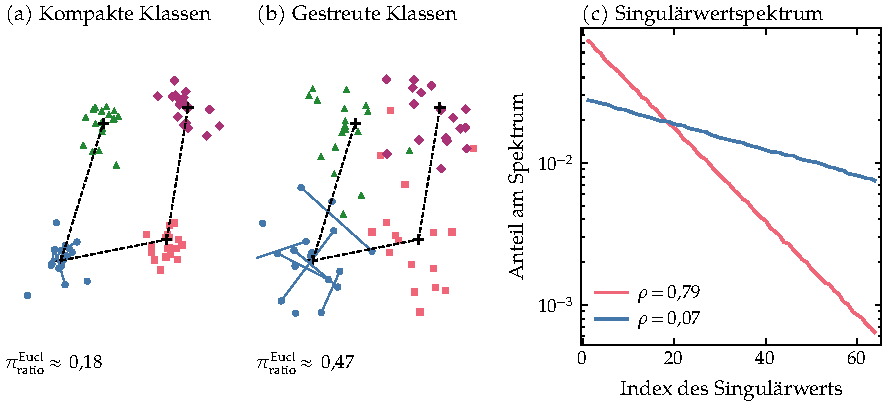
\includegraphics{neu/geometrie_konzept}
  \caption[Maße für die Geometrie eines Embedding-Raums]{Geometriemaße an synthetischen, nicht normierten Daten. (a) und (b)~Vier Klassen mit gleichen Zentren (Kreuze) und unterschiedlicher Streuung, durchgezogen: Abstände innerhalb einer Klasse, gestrichelt: Abstände zwischen Zentren, $\pi_{\mathrm{ratio}}^{\mathrm{Eucl}}$: euklidisches Gegenstück zum Maß aus Gleichung~\eqref{eq:piratio}. (c)~Normierte Singulärwerte zweier 64-dimensionaler Matrizen mit wenigen (rot) und vielen (blau) genutzten Richtungen mit ihrem spektralen Abfall $\rho$. Maße nach~\cite{roth_revisiting_2020}.}
  \label{fig:geometrie:konzept}
\end{figure}

Gemeinsam beschreiben diese Maße, wie stark ein Training den Raum komprimiert und wie weit die Klassen im Verhältnis zu ihrem Abstand streuen~\cite{roth_revisiting_2020}. Kapitel~\ref{chap:ergebnisse} verwendet sie, um die Wirkung der semi-supervised Verfahren über den Trainingsverlauf zu verfolgen.

\section{Vision Transformer und DINOv2}
\label{sec:vit}

Ein \ac{ViT} überträgt die aus der Sprachverarbeitung stammende Transformer-Architektur \cite{vaswani_attention_2017} auf Bilder \cite{dosovitskiy_image_2020}. Seine Eingabe ist eine Folge aus einem zusätzlichen lernbaren \aclu{CLS}-Token (\acs{CLS}-Token) und je einem linear projizierten, positionskodierten Vektor für jeden nicht überlappenden Patch fester Größe. Die Eingabe durchläuft mehrere Transformer-Blöcke mit Self-Attention. Klassifiziert wird anschließend allein anhand des Ausgangs an der Position des \ac{CLS}-Tokens~\cite{dosovitskiy_image_2020}.



DINOv2 bezeichnet eine Familie von \acp{ViT}, die ohne Labels auf einer kuratierten Sammlung von 142 Millionen Bildern (LVD-142M) vortrainiert werden. Das self-supervised Trainingsverfahren basiert dabei unter anderem auf einer Selbstdistillation zwischen einem Student- und einem Teacher-Netz. Als Teacher bei der Destillation des hier verwendeten ViT-B/14 diente das ViT-g. Das ViT-B/14 arbeitet mit Patches zu je $14\times14$ Pixeln und einer Embedding-Dimension von 768 \cite{oquab_dinov2_2023}. Entsprechend ist auch der Ausgabevektor des \ac{CLS}-Tokens, hier die globale Bildrepräsentation, 768-dimensional.

 
Für die Auswertung ist die Zusammensetzung der Vortrainingsdaten wichtig. Bei der Erstellung von LVD-142M dienten unter anderem die ursprünglichen Klassifikations-Trainingssplits von Stanford Cars und \ac{CUB} als Ausgangspunkt für die Auswahl von Webbildern. Über eine clusterbasierte Suche wurden für jeden der beiden Datensätze jeweils eine Million Webbilder aufgenommen~\cite{oquab_dinov2_2023}.

In-Shop und Semi-iNat-2021 dienten nicht als Ausgangsdatensätze dieser Auswahl. Ein linearer Klassifikator auf den eingefrorenen DINOv2-Merkmalen trennt die Klassen von Stanford Cars fast so gut wie die von \ac{CUB}~\cite{oquab_dinov2_2023}.

Für diese Arbeit folgt daraus, dass die Referenzdatensätze für die Auswahl der Vortrainingsbilder auch Bilder jener Automodelle und jener Vogelarten umfassten, die im \ac{DML}-Protokoll als ungesehene Testklassen gelten. Bei Cars196 verteilt der ursprüngliche Split die Bilder jeder Klasse etwa zur Hälfte auf Training und Test~\cite{krause_3d_2013}. Bei \ac{CUB} enthält der offizielle Trainingssplit nach Prüfung seiner Split-Datei in dieser Arbeit ebenfalls Bilder aller 200 Arten \cite{oquab_dinov2_2023}.

Die DINOv2-Modelle werden vor allem anhand ihrer eingefrorenen Merkmale bewertet. Dazu werden lineare Klassifikatoren auf diesen Merkmalen trainiert oder Nearest-Neighbor-Verfahren eingesetzt~\cite{oquab_dinov2_2023}. In dieser Arbeit wird das Backbone eingefroren und nur ein linearer Head mit anschließender Normierung trainiert. Nach Gleichung~\eqref{eq:mahalanobis} lernt das Verfahren damit eine Mahalanobis-artige Gewichtung der vortrainierten Merkmale \cite{weinberger_distance_2009}. Die Verlustfunktionen, das Sampling und das Evaluationsprotokoll übernimmt die Arbeit dennoch aus dem \ac{DML}.

\section{Modellauswahl und Hyperparameteroptimierung}
\label{sec:modellauswahl}

Jedes Trainingsverfahren hat Hyperparameter wie die Lernrate, die Batchgröße oder die Parameter der Verlustfunktion, von deren Werten oft abhängt, wie gut das trainierte Modell wird~\cite{bischl_hyperparameter_2023}. Gewählt werden sie beispielsweise anhand einer Schätzung des Generalisierungsfehlers auf \emph{Validierungsdaten}, die nicht zum Training gehören. Wird dabei der beste Validierungswert selbst als Leistung berichtet, ist diese Schätzung zu optimistisch, weshalb die abschließende Schätzung Testdaten braucht, die in die Auswahl nicht eingegangen sind~\cite{bischl_hyperparameter_2023}. Dasselbe gilt für den Zeitpunkt, zu dem das Training beendet wird~\cite{musgrave_metric_2020}. Beim \emph{Early Stopping} entscheidet deshalb die Validierungsleistung sowohl über das Ende des Trainings als auch über die Epoche, deren Modell getestet wird. Eine Studie zum Training von Retrieval-Modellen beendet es nach einer festen Zahl von Epochen ohne Verbesserung~\cite{berton_all_2025}, die diese Arbeit als \emph{Patience} bezeichnet.

Nach \textcite{musgrave_metric_2020} beruhen viele berichtete Fortschritte des \ac{DML} auf Unterschieden im Versuchsaufbau, etwa auf verschiedenen Backbones, Embedding-Größen und Vorverarbeitungen. Aus Versuchen, in denen die Batchgröße, die Vorverarbeitung, die Architektur und die Embedding-Dimension einzeln variiert werden, folgern auch \textcite{roth_revisiting_2020}, dass schon die Wahl dieser Größen die Ergebnisse stark verschieben kann. Weil die übliche Aufteilung nur Trainings- und Testklassen vorsieht, ist zudem der in den meisten Arbeiten berichtete Testwert zugleich der Wert, nach dem Hyperparameter und Trainingsdauer gewählt wurden~\cite{musgrave_metric_2020}. Die Validierung sollte im \ac{DML} deshalb auf Klassen erfolgen, die nicht für das Training verwendet wurden.

Die \emph{klassendisjunkte Kreuzvalidierung} teilt die Trainingsklassen in $n_{\mathrm{F}}$ Folds, trainiert für jeden Fold ein Modell auf den übrigen Folds und validiert es auf den Klassen des ausgelassenen Folds, wobei der Mittelwert dieser Validierungen die Hyperparametersuche leitet~\cite{musgrave_metric_2020}. Anschließend werden die $n_{\mathrm{F}}$ Modelle dort auf den Testklassen bewertet, einzeln und mit verketteten Embeddings. Abschnitt~\ref{sec:protokoll} beschreibt die Umsetzung in dieser Arbeit.

Bei der beschriebenen Kreuzvalidierung bleiben die Testklassen je Datensatz fest. Der Benchmark ooDML prüft Verfahren dagegen neben der üblichen Aufteilung auf weiteren klassendisjunkten Aufteilungen, deren Trainings- und Testbilder unterschiedlich stark voneinander abweichen, gemessen mit einer Fréchet-Distanz auf den Merkmalen eines ResNet50-Klassifikators. Die stärker verschobenen Aufteilungen, die dort durch den Tausch ganzer Klassen zwischen Training und Test und zuletzt durch das Entfernen weiterer Klassen entstehen, senken die Recall@1 aller untersuchten Verfahren \cite{milbich_characterizing_2021}. 

Es gibt eine Reihe von Suchverfahren, von der Gittersuche und der zufälligen Suche bis zur Bayes'schen Optimierung \cite{bischl_hyperparameter_2023}. 
Da häufig nur wenige Hyperparameter die Leistung stark beeinflussen,
untersucht eine zufällige Suche bei gleicher Zahl von Versuchen
typischerweise mehr unterschiedliche Werte dieser Hyperparameter
als eine Gittersuche \cite{bergstra_random_2012}.
Modellbasierte Verfahren berücksichtigen dagegen die Ergebnisse
bisheriger Versuche, um gezielt neue Konfigurationen auszuwählen
\cite{bischl_hyperparameter_2023}. Der \ac{TPE} teilt dazu die bisherigen Konfigurationen anhand eines Quantils der beobachteten Zielwerte in bessere und übrige, schätzt für beide Gruppen eine eigene Dichte und bevorzugt neue Konfigurationen mit einem hohen Verhältnis der ersten zur zweiten Dichte~\cite{bergstra_algorithms_2011}. Während die ursprüngliche Variante für jeden Hyperparameter eine eigene eindimensionale Dichte schätzt, modelliert die multivariate Variante die Hyperparameter gemeinsam und kann dadurch Abhängigkeiten zwischen ihnen berücksichtigen~\cite{watanabe_tree-structured_2023}.


Für die Frage, welche Hyperparameter die Leistung überhaupt beeinflussen, verwendet diese Arbeit nur die zufälligen Versuche, denn Effektschätzungen, die ein Ersatzmodell aus den Versuchen einer Bayes'schen Optimierung ableitet, können durch deren ungleichmäßige Abtastung des Suchraums verzerrt sein~\cite{moosbauer_explaining_2021}. Liegen viele Konfigurationen innerhalb der Messunsicherheit des besten Versuchs, wird in dieser Arbeit nicht der genaue Wert der gewählten Konfiguration gedeutet, sondern nur der Bereich, in dem gute Werte liegen. Ein ähnlicher Gedanke liegt der Ein-Standardfehler-Regel zugrunde, bei der neben der Validierungsleistung auch die Einfachheit des Modells berücksichtigt wird~\cite{bischl_hyperparameter_2023}.




\chapter{Semi-supervised Verfahren}
\label{chap:ssdml}

\section{Semi-supervised Learning}
\label{sec:ssl}

Das supervised Learning verwendet gelabelte Daten zum Training eines Modells, während das unsupervised Learning ohne vorgegebene Labels auskommt. Das \acl{SSL} hingegen verfolgt eine supervised Aufgabe wie die Klassifikation, nutzt dafür jedoch zusätzlich ungelabelte Daten \cite{van_engelen_survey_2019}. In der Notation dieser Arbeit umfasst der Trainingspool $\mathcal{X}=\{\bm{x}_i\}_{i=1}^{N}$ gelabelte Bilder mit Index in $\mathcal{I}_{\mathrm{L}}$, deren Klassenlabel $y_i\in\{1,\dots,C\}$ bekannt ist. Für die übrigen Bilder mit Index in $\mathcal{I}_{\mathrm{U}}=\{1,\dots,N\}\setminus\mathcal{I}_{\mathrm{L}}$ ist $y_i$ unbekannt. Im Trainingspool kommen $C$ Klassen vor. Die gelabelten Klassen bilden die Menge $\mathcal{C}_{\mathrm{L}}=\{y_i:i\in\mathcal{I}_{\mathrm{L}}\}$. Klassen, die ausschließlich ungelabelt vorkommen, fehlen in $\mathcal{C}_{\mathrm{L}}$, sodass $|\mathcal{C}_{\mathrm{L}}|=C$ nur gilt, wenn jede Klasse gelabelte Bilder hat. Ob ungelabelte Daten helfen, hängt davon ab, wie die Merkmalsverteilung $p(\bm{x})$ mit der bedingten Klassenverteilung $p(y\mid\bm{x})$ zusammenhängt \cite{van_engelen_survey_2019}.

Die Nutzung ungelabelter Daten im \ac{SSL} beruht auf Annahmen über die Struktur und Verteilung der Daten. Die \emph{Smoothness-Annahme} besagt, dass nahe beieinanderliegende Punkte im Eingaberaum dasselbe Label haben sollten. Nach der \emph{Mannigfaltigkeitsannahme} gehören Punkte auf derselben niedrigdimensionalen Mannigfaltigkeit zur gleichen Klasse. Die \emph{Low-Density-Annahme} besagt dagegen, dass Entscheidungsgrenzen durch Bereiche geringer Datendichte verlaufen sollten \cite{van_engelen_survey_2019}. Die Übersicht beschreibt diese drei Annahmen als spezielle Formen der \emph{Cluster-Annahme}, nach der Punkte desselben Clusters zur gleichen Klasse gehören \cite{van_engelen_survey_2019}. Abbildung \ref{fig:ssl:annahmen} veranschaulicht, welche ungelabelten Punkte unter den jeweiligen Annahmen derselben Klasse zugeordnet werden.

\begin{figure}[tbp]
  \centering
  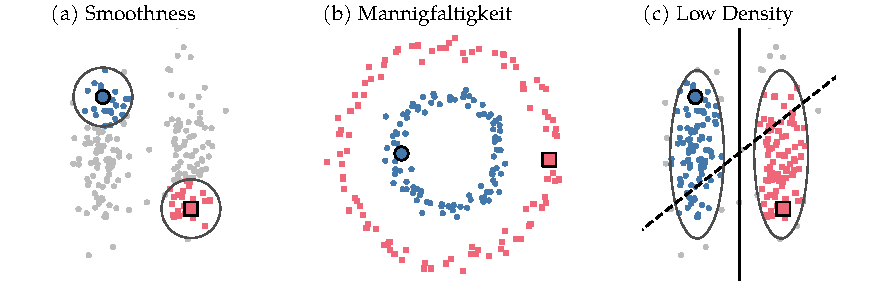
\includegraphics{neu/ssl_annahmen}
  \caption[Annahmen des \acs{SSL} an synthetischen Daten]{Annahmen des \acs{SSL} an synthetischen Daten nach \cite{van_engelen_survey_2019}. Groß und schwarz umrandet: gelabelte Punkte. Farbig: ungelabelte Punkte, die nach der Annahme dem gelabelten Punkt derselben Farbe ähneln, grau: übrige. (a) Kreise: Umgebungen der gelabelten Punkte. (c) Ellipsen: Bereiche hoher Dichte bis zu zwei Standardabweichungen um die Klassenmitten, durchgezogen: eine Entscheidungsgrenze im Bereich geringer Dichte, gestrichelt: Mittelsenkrechte der gelabelten Punkte als Grenze ohne ungelabelte Punkte.}
  \label{fig:ssl:annahmen}
\end{figure}

In dieser Arbeit gelten die Annahmen nicht im Eingaberaum der Rohbilder, sondern in dem Raum, in dem die Ähnlichkeit gemessen wird. Ein ungelabeltes Foto eines Automodells kann nur dann über seine Nachbarn einer Klasse zugeordnet werden, wenn diese Nachbarn im Merkmals- oder Embedding-Raum überwiegend dasselbe Automodell zeigen. Ob das zutrifft, hängt von der Datenverteilung und von der Repräsentation ab. Zu Beginn des Trainings ist daher entscheidend, wie gut das vortrainierte Modell die Trainingsklassen bereits trennt. Die Annahmen müssen deshalb im konkreten Fall geprüft werden. Im \ac{DML} kommt eine weitere Annahme hinzu. Was ein Modell an den ungelabelten Bildern lernt, bei Autos etwa eine geringere Empfindlichkeit gegenüber dem Blickwinkel, der Lackfarbe und dem Hintergrund, muss sich auf ungesehene Klassen übertragen.

Ein \emph{induktives} Verfahren lässt sich anders als ein \emph{transduktives} ohne weiteres Training auf neue Daten anwenden \cite{van_engelen_survey_2019}. Für diese Arbeit ist entscheidend, dass \ac{DML} ein induktives Modell verlangt, denn getestet wird auf Bildern oder sogar Klassen, die im Training nicht vorkamen. Ein transduktiver Baustein kann aber Teil eines induktiven Verfahrens sein. Bei der Übertragung auf tiefe Netze dient \ac{LP} als transduktiver Zwischenschritt, der den ungelabelten Beispielen Pseudo-Labels zuweist. Mit diesen wird anschließend ein induktives Modell trainiert \cite{iscen_label_2019}.

Induktive Verfahren werden danach unterschieden, wie die ungelabelten Daten in sie eingehen. Bei der \emph{unsupervised Vorverarbeitung} werden sie in einem eigenen Schritt vor dem supervised Training genutzt, beispielsweise zum Vortraining neuronaler Netze. \emph{Wrapper-Verfahren} weisen den ungelabelten Daten dagegen Pseudo-Labels zu, um sie anschließend für das supervised Training zu nutzen. \emph{Intrinsisch semi-supervised Verfahren} erweitern das Lernverfahren selbst, etwa um einen zusätzlichen Term im Trainingsziel \cite{van_engelen_survey_2019}. Bei neuronalen Netzen lassen sich ungelabelte Daten so über einen gewichteten Regularisierungsterm einbeziehen, der zur supervised Verlustfunktion hinzukommt \cite{weston_deep_2012, hoffer_semi-supervised_2018}. In der Notation dieser Arbeit lautet ein solches Trainingsziel \cite{weston_deep_2012, hoffer_semi-supervised_2018}
\begin{equation}
  \mathcal{L}=\mathcal{L}_{\mathrm{sup}}+w_{\mathrm{reg}}\,\mathcal{L}_{\mathrm{reg}}.
  \label{eq:ssl:ziel}
\end{equation}
Dabei ist $\mathcal{L}_{\mathrm{sup}}$ eine \ac{DML}-Verlustfunktion aus Abschnitt \ref{sec:verluste} auf den gelabelten Bildern. Der \ac{SSL}-Term $\mathcal{L}_{\mathrm{reg}}$ bezieht die ungelabelten Bilder ein und $w_{\mathrm{reg}}\ge0$ ist sein Gewicht. DINOv2 wurde mit Self-supervised Learning auf externen Daten vortrainiert, was einer unsupervised Vorverarbeitung entspricht \cite{oquab_dinov2_2023}. In dieser Arbeit liefert dieses Vortraining die festen Merkmale für alle Experimente.

Zu den drei Gruppen gehören weitere Verfahren, etwa das Co-Training, störungsbasierte Ansätze wie Mean Teacher, generative Modelle und Semi-supervised Support Vector Machines \cite{van_engelen_survey_2019}. 

\section{Evaluation von semi-supervised Verfahren}
\label{sec:ssl:evaluation}

Wie groß der Vorteil von \ac{SSL} in der Bildklassifikation unter vergleichbaren Versuchsbedingungen ausfällt, wurde mit mehreren \ac{SSL}-Verfahren bei derselben Netzarchitektur und einem einheitlichen Trainingsablauf in einer Vergleichsarbeit untersucht. Sowohl die supervised Baseline als auch jedes \ac{SSL}-Verfahren wurden mit jeweils 1000 Versuchen zur Hyperparameteroptimierung abgestimmt. Unter diesen Bedingungen reduzierte zum Beispiel das $\Pi$-Model den Testfehler auf CIFAR-10 mit 4000 Labels von \qty{20.26}{\percent} auf \qty{16.37}{\percent}. Dieselbe Studie stellt dem einen früher berichteten Rückgang von \qty{34.85}{\percent} auf \qty{12.36}{\percent} gegenüber, der von einer deutlich schwächeren supervised Baseline ausging. Ein Netz, das zunächst auf ImageNet vortrainiert und anschließend mit 4000 gelabelten CIFAR-10-Bildern angepasst wurde, erreichte einen geringeren Testfehler als alle untersuchten \ac{SSL}-Verfahren derselben Architektur \cite{oliver_realistic_2018}.

Auch die Validierungsmenge entscheidet darüber, wie aussagekräftig ein Vergleich ist. Auf SVHN standen in vielen Arbeiten nur 1000 gelabelten Trainingsbildern rund 7000 gelabelte Validierungsbilder gegenüber, ein Verhältnis, das in der Praxis kaum vorkommt. Bei 100 Validierungsbildern schwankten die geschätzten Fehlerraten dagegen so stark, dass sich die Verfahren kaum noch zuverlässig vergleichen ließen. Außerdem kann \ac{SSL} schlechter abschneiden als die supervised Baseline, wenn die ungelabelten Daten Klassen ohne gelabelte Beispiele enthalten. Das zeigte ein Versuch mit den sechs Tierklassen von CIFAR-10 als gelabelter Aufgabe und zusätzlich mit ungelabelten Daten aus vier Klassen, von denen schrittweise weniger zu den gelabelten gehörten. Im Extremfall stammten sie nur aus den vier Fahrzeugklassen. Die Hyperparameter wurden für diesen Versuch allerdings nicht neu gesucht \cite{oliver_realistic_2018}.

In diesen Versuchen näherten sich die Verfahren mit wachsender Zahl der Labels einander an, wobei sie mit wenigen Labels am weitesten auseinander lagen. Über Datensätze mit unterschiedlich vielen Klassen hinweg lässt sich das Label-Budget als Zahl gelabelter Bilder je Klasse vergleichen. Die 4000 Labels, mit denen Verfahren auf CIFAR-10 häufig getestet wurden, entsprechen 400 Bildern je Klasse \cite{oliver_realistic_2018}. Im \ac{SSDML} wurden für Cars196 und \ac{CUB} dagegen jeweils nur fünf Bilder je Klasse verwendet \cite{dutta_semi-supervised_2021, zhuang_deep_2021}.

Die Frage nach Klassen, die nur im ungelabelten Pool vorkommen, ist inzwischen differenzierter beantwortet. In vielen früheren Versuchen blieb die Zahl der ungelabelten Bilder fest, sodass ein größerer Anteil unbekannter Klassen zugleich weniger ungelabelte Bilder bekannter Klassen bedeutete. Ohne diese Kopplung sank die Genauigkeit der meisten Verfahren mit wachsendem Anteil unbekannter Klassen weiterhin, aber unterschiedlich stark \cite{he_reevaluating_2025}. Auf den fine-grained Datensätzen Semi-Aves und Semi-Fungi kamen Bilder weiterer Arten zu den ungelabelten Bildern bekannter Arten hinzu. Ohne Vortraining halfen zusätzliche ungelabelte Daten aus unbekannten Klassen bei einigen Verfahren. Bei vortrainierten Modellen verschlechterten sie dagegen häufig die Ergebnisse \cite{su_realistic_2021}. Für Hypothese H3 aus Kapitel \ref{chap:einleitung} folgt daraus zweierlei. Ein Befund zu H3 hängt davon ab, ob Bilder fremder Klassen ungelabelte Bilder bekannter Klassen ersetzen oder zu ihnen hinzukommen. Außerdem ist ein Schaden nach diesen Befunden bei einem vortrainierten Modell wie DINOv2 eher zu erwarten als ohne Vortraining. 

Mit stark vortrainierten \ac{ViT}-Modellen stellt sich die Frage nach dem Nutzen ungelabelter Daten neu. Auf Benchmarks wie CIFAR-10 genügt bereits ein linearer Klassifikator auf eingefrorenen Merkmalen, um mit wenigen Labels eine hohe Genauigkeit zu erreichen. Klassische \ac{SSL}-Verfahren erzielten gegenüber rein supervised Fine-Tuning-Verfahren jedoch auch auf schwierigeren Aufgaben oft nur geringe Leistungsgewinne. Auf anspruchsvolleren Aufgaben liefert parametereffizientes Fine-Tuning allein mit gelabelten Daten häufig bessere Ergebnisse als die untersuchten \ac{SSL}-Verfahren. Durch die Kombination der Pseudo-Labels verschiedener solcher Modelle lassen sich dort jedoch zusätzliche Gewinne mit ungelabelten Daten erzielen \cite{zhang_revisiting_2025}. Ob diese Befunde für das \ac{DML} mit ungesehenen Testklassen gelten, ist offen.

\section{Entropieminimierung, Pseudo-Labels und Self-Training}
\label{sec:selftraining}

\subsection{Entropieminimierung und Pseudo-Labels}
\label{sec:entropie}

Ausgangspunkt der Entropieminimierung ist, dass ein ungelabelter Punkt in der bedingten Log-Likelihood wegen $\sum_{c\in\mathcal{C}_{\mathrm{L}}}p_{ic}=1$ mit $p_{ic}=p(c\mid\bm{x}_i;\bm{\theta})$ nur den Summanden $\log 1=0$ beiträgt \cite{grandvalet_semi-supervised_2005}. Das Verfahren ergänzt die negative bedingte Log-Likelihood der gelabelten Punkte, die dort die Rolle von $\mathcal{L}_{\mathrm{sup}}$ in Gleichung \eqref{eq:ssl:ziel} übernimmt, um einen \ac{SSL}-Term, in der Notation dieser Arbeit \cite{grandvalet_semi-supervised_2005}
\begin{equation}
  \mathcal{L}_{\mathrm{reg}}^{\mathrm{Ent}}=-\sum_{i\in\mathcal{I}_{\mathrm{U}}}\sum_{c\in\mathcal{C}_{\mathrm{L}}}p_{ic}\log p_{ic}.
  \label{eq:entmin}
\end{equation}
Der Term minimiert die Entropie der Klassenvorhersagen für ungelabelte Datenpunkte und begünstigt damit eine hohe Konfidenz bei der Zuordnung zu einer Klasse. Bei einem ausreichend regularisierten Modell kann die Konfidenz nahe der Entscheidungsgrenze nicht beliebig hoch sein. Die Entropieminimierung begünstigt daher Entscheidungsgrenzen in Bereichen geringer Datendichte und folgt damit der Low-Density-Annahme \cite{grandvalet_semi-supervised_2005}.

Pseudo-Labeling kommt ohne eigenen Entropieterm aus. Für die ungelabelten Bilder eines Batches wird bei jeder Gewichtsaktualisierung die jeweils wahrscheinlichste Klasse zum One-hot-Ziel. Der supervised Verlust behandelt dieses Pseudo-Label wie ein echtes Label. Der Verlustterm der ungelabelten Bilder erhält aber ein eigenes Gewicht, das zunächst null ist und dann linear auf einen Endwert steigt. Gedeutet wird dieses Vorgehen dort als eine Form der Entropieminimierung \cite{lee_pseudo-label_2013}.

\subsection{Self-Training und Teacher-Student}
\label{sec:teacher-student}

Beim \emph{Self-Training} erweitert ein Modell seine gelabelte Trainingsmenge aus den eigenen Vorhersagen, denn nach jeder Runde gelten ausgewählte Vorhersagen für ungelabelte Daten, etwa die mit der höchsten Konfidenz, als Pseudo-Labels der nächsten Runde \cite{yarowsky_unsupervised_1995, van_engelen_survey_2019}. Das Risiko solcher Verfahren, der \emph{Confirmation Bias}, liegt darin, dass sich falsche Pseudo-Labels festsetzen, weil das Modell aus seinen eigenen Fehlern lernt. Mixup und genügend gelabelte Bilder in jedem Batch brachten Pseudo-Labeling in den dortigen Versuchen zur Bildklassifikation auf das Niveau der Konsistenzregularisierung oder darüber \cite{arazo_2020}.

Bei Noisy Student erzeugt in jeder Runde das zuletzt trainierte Modell als Teacher die Pseudo-Labels, aus denen ein neuer Student lernt. Rauschen in Form von Augmentierung, Dropout und stochastischer Tiefe wirkt dabei beim Training beider Modelle, nicht aber beim Erzeugen der Pseudo-Labels \cite{xie_self-training_2019}. Mean Teacher gehört zur Konsistenzregularisierung, bei der ein Modell für verschiedene Störungen desselben Bildes dieselbe Vorhersage liefern soll. Dessen Teacher ist kein getrennt trainiertes Modell, sondern ein \ac{EMA} der Student-Gewichte, $\bm{\theta}'\leftarrow\beta\,\bm{\theta}'+(1-\beta)\,\bm{\theta}$ mit $\beta$ nahe eins. Der Student wird so trainiert, dass seine Vorhersage möglichst wenig von der des Teachers abweicht \cite{tarvainen_weight-averaged_2017}. FixMatch verbindet Pseudo-Labels und Konsistenzregularisierung über zwei unterschiedlich stark augmentierte Ansichten desselben ungelabelten Bildes und eine Konfidenzschwelle \cite{sohn_fixmatch_2020}.

Mean Teacher und FixMatch verlangen mit ihrem Konsistenzterm keine gleichen Labels für nahe Bilder, sondern gleiche Vorhersagen für veränderte Fassungen desselben Bildes \cite{tarvainen_weight-averaged_2017, sohn_fixmatch_2020}. Das entspricht der bei Bildern üblichen, abgeschwächten Form der Smoothness-Annahme \cite{van_engelen_survey_2019}. 

\section{Graphbasierte Verfahren}
\label{sec:graph}

\subsection{Graphen und Laplace-Matrix}

Die folgende Darstellung der Graphkonstruktion orientiert sich an der Übersicht in \textcite{van_engelen_survey_2019}. Graphbasierte Verfahren repräsentieren gelabelte und ungelabelte Punkte als Knoten eines Graphen, dessen Kanten Ähnlichkeiten beschreiben. Die Gewichtsmatrix $\bm{W}\in\mathbb{R}^{N\times N}$ enthält für jede Kante ein nichtnegatives Gewicht $W_{ij}$ und für alle übrigen Paare null. Verbreitet sind \ac{kNN}-Graphen, in denen jeder Punkt mit seinen $k_{\mathrm{NN}}$ nächsten Nachbarn verbunden ist. Weil diese Beziehung nicht symmetrisch ist, wird für eine Kante entweder verlangt, dass einer der beiden Punkte zu den Nachbarn des anderen zählt, oder dass beide wechselseitig Nachbarn sind \cite{van_engelen_survey_2019}. Die Gewichte sind beispielsweise binär \cite{hoi_semi-supervised_2010} oder ergeben sich über einen Kern aus der Distanz, etwa $W_{ij}=\exp(-\gamma\lVert\bm{x}_i-\bm{x}_j\rVert_2^2)$ \cite{van_engelen_survey_2019}. Im Folgenden sind die Graphen ungerichtet, also $\bm{W}=\bm{W}^{\top}$, ohne Selbstkanten ($W_{ii}=0$). Die Gradmatrix $\bm{D}$ ist diagonal mit den Knotengraden $D_{ii}=\sum_j W_{ij}$ und die Graph-Laplace-Matrix ist $\bm{L}=\bm{D}-\bm{W}$. Summiert über die Spalten einer Matrix $\bm{F}\in\mathbb{R}^{N\times|\mathcal{C}_{\mathrm{L}}|}$ ergibt die quadratische Form von $\bm{L}$ den \emph{Laplace-Term} \cite{hoi_semi-supervised_2010, belkin_manifold_2006}
\begin{equation}
  \operatorname{tr}(\bm{F}^{\top}\bm{L}\bm{F})=\tfrac{1}{2}\sum_{i,j}W_{ij}\,\lVert\bm{F}_{i:}-\bm{F}_{j:}\rVert_2^2 .
  \label{eq:laplace}
\end{equation}
Der Term ist klein, wenn verbundene Knoten ähnliche Zeilen in $\bm{F}$ haben. Damit begünstigt er ähnliche Vorhersagen für benachbarte Punkte und folgt der Smoothness-Annahme. Da der Graph auch weiter entfernte Punkte über mehrere Kanten verbinden kann, lässt sich die Glättung entlang der durch den Graphen angenäherten Mannigfaltigkeitsstruktur fortsetzen \cite{zhou_learning_2003, belkin_manifold_2006, van_engelen_survey_2019}. Auf den Knoten mit positivem Grad vergleicht die symmetrisch normierte Variante $\bm{L}_{\mathrm{sym}}=\bm{I}-\bm{D}^{-1/2}\bm{W}\bm{D}^{-1/2}$ die mit $1/\sqrt{D_{ii}}$ skalierten Zeilen von $\bm{F}$ \cite{zhou_learning_2003, belkin_manifold_2006}. Ohne die Normierung können Knoten mit vielen oder starken Kanten einen größeren Einfluss auf den Laplace-Term haben. Die Skalierung mit $1/\sqrt{D_{ii}}$ dämpft diesen Einfluss \cite{van_engelen_survey_2019}. Für diese Arbeit ist entscheidend, wie viele Kanten eines Graphen innerhalb einer Klasse verlaufen. Verbindet er Bilder ähnlicher, aber verschiedener Klassen, verlangt der Laplace-Term ähnliche Werte genau dort, wo die Labels wechseln.

\subsection{Label Propagation}
\label{sec:lp}

Label Propagation überträgt Labelinformationen entlang der Kanten auf ungelabelte Knoten. Jeder Knoten erhält wiederholt die mit den Kantengewichten gewichteten Label-Scores seiner Nachbarn, die Scores werden normiert und die gelabelten Knoten werden nach jedem Schritt auf ihr bekanntes Label zurückgesetzt \cite{zhu_learning_2002}. Bei der Variante mit lokaler und globaler Konsistenz bleiben die Label-Scores der gelabelten Knoten veränderlich. Ein quadratischer Strafterm bestraft Abweichungen von den Ausgangslabels \cite{zhou_learning_2003}. Dadurch kann das Verfahren weniger empfindlich auf fehlerhafte Labels reagieren als die klassische Label Propagation mit festgehaltenen Labels. Diese Variante wird auch als Label Spreading bezeichnet \cite{van_engelen_survey_2019,pedregosa_scikit-learn_2011}. Die Matrix $\bm{Y}\in\mathbb{R}^{N\times|\mathcal{C}_{\mathrm{L}}|}$ enthält die One-hot-Labels der gelabelten Knoten. Jede Spalte entspricht einer Klasse $c\in\mathcal{C}_{\mathrm{L}}$. Die Zeilen der ungelabelten Knoten enthalten nur Nullen. Mit $\bm{S}=\bm{D}^{-1/2}\bm{W}\bm{D}^{-1/2}$ und $0<\alpha<1$ wird dort \cite{zhou_learning_2003}
\begin{equation}
  \bm{F}^{(t+1)}=\alpha\bm{S}\bm{F}^{(t)}+(1-\alpha)\bm{Y}
  \quad\xrightarrow{t\to\infty}\quad
  \bm{F}^{*}=(1-\alpha)(\bm{I}-\alpha\bm{S})^{-1}\bm{Y}
  \label{eq:lp}
\end{equation}  
iteriert. Je näher $\alpha$ an eins liegt, desto stärker hängen die Label-Scores von den Nachbarn ab und desto schwächer hängen sie von den Ausgangslabels ab, die in jedem Schritt mit dem Gewicht $1-\alpha$ eingehen. Das Pseudo-Label eines ungelabelten Knotens entspricht der Klasse mit dem größten Wert in seiner Zeile von $\bm{F}^{*}$. Der Fixpunkt minimiert eine Zielfunktion aus dem Laplace-Term mit $\bm{L}_{\mathrm{sym}}$ und der quadratischen Abweichung von $\bm{Y}$ \cite{zhou_learning_2003}.

Verlaufen zwischen den Klassen wenige Kanten, können Labels entlang einer Mannigfaltigkeit auch Punkte derselben Klasse erreichen, die weit von jedem gelabelten Punkt entfernt sind. Wo zwei Klassen ineinander übergehen, gelangen Labels leicht über die verbindenden Kanten in die falsche Klasse. Nur auf der Indexmenge $\mathcal{I}_{+}=\{i:\sum_{c\in\mathcal{C}_{\mathrm{L}}}F^{*}_{ic}>0\}$ entsteht durch $p_{ic}=F^{*}_{ic}/\sum_{c'\in\mathcal{C}_{\mathrm{L}}}F^{*}_{ic'}$ eine Verteilung \cite{iscen_label_2019}. Mit $0\log0=0$ lautet die Konfidenz für $|\mathcal{C}_{\mathrm{L}}|>1$ in der Notation dieser Arbeit \cite{iscen_label_2019}
\begin{equation}
  \omega_i=1-\frac{H(\bm{p}_i)}{\log|\mathcal{C}_{\mathrm{L}}|},\qquad H(\bm{p}_i)=-\sum_{c\in\mathcal{C}_{\mathrm{L}}}p_{ic}\log p_{ic}.
  \label{eq:lp-weight}
\end{equation}
Sie ist bei einer Gleichverteilung null und bei einer eindeutigen Zuordnung eins. Eine Verteilung auf mehrere Klassen senkt sie, bei vielen bekannten Klassen kann aber schon eine Verteilung auf nur zwei Klassen einen hohen Wert ergeben. Ein hoher Wert von $\omega_i$ ist deshalb kein Nachweis eines richtigen Pseudo-Labels. Auch falsche Pseudo-Labels erreichten in der ursprünglichen Arbeit hohe Werte. Die Konfidenz wird dort zusätzlich so zu $\tilde\omega_i$ skaliert, dass ihr Maximum über alle Bilder eins ist. Diese vorherige Arbeit, die \acl{LP} auf tiefe Netze überträgt, bezeichnet die Propagation als Diffusion und lässt sie mit dem Training abwechseln \cite{iscen_label_2019}. Nach einem supervised Warm-up werden dort alle Trainingsbilder eingebettet und aus den Embeddings entsteht ein dünner Graph, in der Notation dieser Arbeit mit \cite{iscen_label_2019}
\begin{equation}
  \hat{W}_{ij}=[s_{ij}]_+^{\xi}\ \text{für } j\in\mathcal{V}_{k_{\mathrm{NN}}}(i),\qquad \bm{W}=\hat{\bm{W}}+\hat{\bm{W}}^{\top}.
  \label{eq:lp-graph}
\end{equation}
Dabei ist $\mathcal{V}_{k_{\mathrm{NN}}}(i)$ die Menge der $k_{\mathrm{NN}}$ nächsten Nachbarn von $i$ ohne $i$ selbst. Alle übrigen Einträge von $\hat{\bm{W}}$ sind null. Der Parameter $\xi$ ist ein Exponent, der hohe Ähnlichkeiten betont. Das Verfahren der konjugierten Gradienten löst dort das lineare System $(\bm{I}-\alpha\bm{S})\bm{F}=\bm{Y}$, ohne die dicht besetzte Inverse aus Gleichung \eqref{eq:lp} zu bilden, die bei großen Graphen nicht praktikabel ist. Aus der zeilennormierten Lösung ergeben sich das Pseudo-Label $\hat{y}_i=\argmax_{c\in\mathcal{C}_{\mathrm{L}}}p_{ic}$ und die Konfidenz $\omega_i$ \cite{iscen_label_2019}. Der Faktor $1-\alpha$ aus Gleichung \eqref{eq:lp} wird bei der Klassifikation weggelassen \cite{zhou_learning_2003,iscen_label_2019}. Die ursprüngliche Arbeit zur Anwendung von \ac{LP} auf tiefe Netze trainiert das Netz anschließend mit einer gewichteten Kreuzentropie auf gelabelten und pseudo-gelabelten Bildern. Die Gewichte gleichen unterschiedlich große Klassen aus und dämpfen zusätzlich unsichere Pseudo-Labels über die Konfidenz $\omega_i$. Der Graph und die Pseudo-Labels werden nach jeder Epoche aus den aktualisierten Embeddings neu berechnet und die vorherige Arbeit verwendet $k_{\mathrm{NN}}=50$, $\xi=3$ und $\alpha=\num{0.99}$ \cite{iscen_label_2019}.

\subsection{Graph-Regularisierung tiefer Netze}
\label{sec:weston}

Statt Labels über einen Graphen zu verteilen, kann der Laplace-Term aus Gleichung \eqref{eq:laplace} auch direkt als Regularisierer dienen. Die Mannigfaltigkeitsregularisierung ergänzt eine Zielfunktion um einen gewichteten Term $\operatorname{tr}(\bm{F}^{\top}\bm{L}\bm{F})$. Dabei enthält $\bm{F}$ die Vorhersagen für alle gelabelten und ungelabelten Datenpunkte. Der Term bestraft unterschiedliche Vorhersagen auf stark verbundenen Graphknoten. Dadurch wird eine Vorhersagefunktion begünstigt, die entlang der durch den Graphen approximierten Geometrie der Daten glatt verläuft \cite{belkin_manifold_2006}.

Die Embedding-Regularisierung überträgt diese Idee auf tiefe Netze. Sie addiert zum supervised Verlust eine Variante des Contrastive Loss aus Abschnitt \ref{sec:verluste:paare}, deren anziehender Teil auf im Graphen verbundene Paare und deren abstoßender Teil auf Paare ohne Kante wirkt. Ohne den abstoßenden Teil wäre dieser Verlust auf den ungelabelten Paaren schon mit $d_{ij}=0$ für alle Paare minimal. Abwechselnd erhalten ein gelabeltes Beispiel einen Schritt auf dem supervised Verlust, ein benachbartes Paar aus dem Graphen einen Schritt auf dem anziehenden Teil und ein Paar mit einem zufällig gezogenen ungelabelten Beispiel einen Schritt auf dem abstoßenden Teil \cite{weston_deep_2012}.

\section{Semi-supervised Metric Learning}
\label{sec:ssml}

\subsection{Graph-Regularisierung einer Metrik}
\label{sec:lrml}

\ac{LRML} verwendet den Laplace-Term als Regularisierer für eine Mahalanobis-Metrik. Aus allen gelabelten und ungelabelten Punkten wird dort mit der euklidischen Distanz ein ungewichteter \ac{kNN}-Graph gebaut, in dem $W_{ij}=1$ gilt, wenn $i$ unter den $k_{\mathrm{NN}}$ nächsten Nachbarn von $j$ ist oder umgekehrt. Die Metrik soll benachbarte Punkte auch nach der Transformation nahe beieinander halten. In der Notation dieser Arbeit lautet der Regularisierer \cite{bellet_survey_2014, hoi_semi-supervised_2010}
\begin{equation}
  \mathcal{L}_{\mathrm{reg}}^{\mathrm{LRML}}(\bm{M})=\tfrac{1}{2}\sum_{i,j}W_{ij}\,d_{\bm{M}}^{2}(\bm{x}_i,\bm{x}_j)=\operatorname{tr}(\bm{X}\bm{L}\bm{X}^{\top}\bm{M}).
  \label{eq:lrml}
\end{equation}
Dabei ist $\bm{X}=[\bm{x}_1,\dots,\bm{x}_N]$ die Matrix mit den Datenpunkten als Spalten. Die Gleichung gilt für $\bm{L}=\bm{D}-\bm{W}$. Für die Anwendung ist dort auch $\bm{L}_{\mathrm{sym}}$ vorgesehen, mit der die Retrieval-Experimente bei $k_{\mathrm{NN}}=6$ rechnen \cite{hoi_semi-supervised_2010}. Der Regularisierer wird mit zwei Termen für gelabelte Paare kombiniert, die die Abstände ähnlicher Paare verkleinern und die Abstände unähnlicher Paare vergrößern. Der Laplace-Term selbst verwendet keine Labels, sondern begünstigt kleine Abstände zwischen Graphnachbarn. Damit orientiert sich \ac{LRML} an der Smoothness-Annahme und berücksichtigt über den Nachbarschaftsgraphen die lokale Datenstruktur im Sinne der Mannigfaltigkeitsannahme aus Abschnitt \ref{sec:ssl} \cite{bellet_survey_2014, hoi_semi-supervised_2010}.

Neben \ac{LRML} wurden weitere Verfahren entwickelt, die die Struktur ungelabelter Daten beim Metric Learning berücksichtigen. Diese unterscheiden sich unter anderem in der Konstruktion des Nachbarschaftsgraphen und in der Wahl des Mannigfaltigkeitsregularisierers \cite{bellet_survey_2014}. Einer der Ansätze bestimmt beispielsweise zunächst, wie sich jeder Datenpunkt
im ursprünglichen Merkmalsraum aus seinen nächsten Nachbarn
rekonstruieren lässt. Ein Regularisierungsterm bestraft
anschließend Abweichungen von diesen Rekonstruktionsbeziehungen
im transformierten Raum \cite{baghshah_semi-supervised_2009}.

Es gibt noch weitere Verfahren, von denen hier einige aufgezählt werden. Das Verfahren \ac{RSSML} erweitert die Laplace-Regularisierung um Gauß-Ähnlichkeiten zwischen benachbarten Punkten und Dichtegewichte. Der Regularisierer wird mit einem Triplet-Hinge-Verlust kombiniert \cite{wang_semi-supervised_2012}. Ein späteres Verfahren übernimmt die dichtegewichtete Regularisierung, ersetzt den Hinge-Verlust jedoch durch einen glatten Triplet-Verlust mit adaptiver Gewichtung der klasseninternen und der klassenübergreifenden Abstände \cite{ying_manifold_2018}. Für Aufnahmen mit \ac{PolSAR} wird ein tiefes Metrik-Netz mit einem Regularisierer trainiert, der quadrierte Distanzen zu den $k_{\mathrm{NN}}$ nächsten Nachbarn mit abstandsabhängigen Gewichten in den Verlust aufnimmt \cite{liu_semi-supervised_2020}.

Andere Erweiterungen beziehen die gelabelten Daten stärker in die Graphkonstruktion ein. \ac{SLRML} kombiniert einen \ac{kNN}-Graphen mit zusätzlichen Kanten zwischen gelabelten Punkten derselben Klasse. Die beiden Gewichtsmatrizen werden addiert, sodass gleich gelabelte Nachbarn ein höheres Kantengewicht erhalten. Darauf baut \ac{SLRMML} als Erweiterung für Daten mit mehreren Modalitäten auf \cite{liang_semisupervised_2022}.

Schwache Ausgangsrepräsentationen sind für \ac{LRML} und verwandte Verfahren ein Risiko, weil deren Graph vor dem Lernen der Metrik feststeht und später nicht mehr korrigiert wird \cite{dutta_semi-supervised_2021}. Für diese Arbeit ist daher relevant, dass sich die Nachbarschaften verändern können, wenn der Graph während des Trainings wiederholt neu aufgebaut wird. Dadurch kann sich die lokale Struktur verbessern, es können aber auch fehlerhafte Nachbarschaften entstehen.

\subsection{Entropiebasierte Verfahren}
\label{sec:hoffer}

Die Entropieminimierung aus Abschnitt \ref{sec:entropie} setzt für jeden Datenpunkt eine Wahrscheinlichkeitsverteilung über die möglichen Klassen voraus. Bei einem reinen Embedding-Modell liegt eine solche Verteilung nicht unmittelbar vor. Das in dieser Arbeit nach seinem Erstautor kurz als Hoffer bezeichnete Verfahren verwendet für jede bekannte Klasse $c\in\mathcal{C}_{\mathrm{L}}$ ein gelabeltes Referenzbild $\bm{x}^{\mathrm{ref}}_c$ \cite{hoffer_semi-supervised_2018}. Für ein Bild $\bm{x}_i$ definiert es in der Notation dieser Arbeit die Verteilung \cite{hoffer_semi-supervised_2018}
\begin{equation}
  p_{ic}=\frac{\exp\bigl(-\lVert\Phi(\bm{x}_i)-\Phi(\bm{x}^{\mathrm{ref}}_c)\rVert_2^2\bigr)}{\sum_{c'\in\mathcal{C}_{\mathrm{L}}}\exp\bigl(-\lVert\Phi(\bm{x}_i)-\Phi(\bm{x}^{\mathrm{ref}}_{c'})\rVert_2^2\bigr)}.
  \label{eq:hoffer}
\end{equation}
Für gelabelte Bilder wird die Kreuzentropie zur richtigen Klasse minimiert, für ungelabelte die Entropie $H(\bm{p}_i)$. Das Verfahren begünstigt somit, dass ein ungelabeltes Bild im Embedding-Raum einem der gelabelten Referenzbilder näher liegt als den übrigen Referenzbildern. Das Verfahren folgt somit wie die Entropieminimierung in Abschnitt \ref{sec:entropie} der Cluster-Annahme. Da die Verteilung ausschließlich über bekannte Klassen gebildet wird, werden auch Bilder unbekannter Klassen zu einer möglichst eindeutigen Zuordnung gedrängt. Da die Embeddings in der ursprünglichen Arbeit nicht normiert werden, kann das Netz die Abstände durch die Skalierung ihrer Normen verändern \cite{hoffer_semi-supervised_2018}.

Derselbe Gedanke liegt \ac{ISMLP} zugrunde. Das Verfahren ersetzt die gelabelten Referenzbilder durch mehrere Proxy-Vektoren, die gemeinsam mit einer Mahalanobis-Metrik gelernt werden. Die Entropie der aus den Abständen zu diesen Proxys gebildeten Verteilung wird für ungelabelte Daten minimiert \cite{chen_efficient_2023}. \ac{SERAPH} minimiert dagegen auf ungelabelten Paaren die Entropie der Wahrscheinlichkeit, mit der ein Paar als ähnlich oder unähnlich gilt \cite{niu_information-theoretic_2012}.

\section{Semi-supervised Deep Metric Learning}
\label{sec:ssdml}

Zwei Arbeiten begründen ihren Ansatz mit einer Lücke. Die eine setzt daran an, dass ungelabelte Daten im \ac{DML} damals selten genutzt wurden. Sie ergänzt deshalb einen gelabelten Datensatz um ungelabelte Bilder eines anderen Datensatzes \cite{duan_slade_2021}. Die andere Arbeit hat festgestellt, dass sich die bisherige Forschung zum semi-supervised Metric Learning auf einige wenige Verfahren zum Lernen linearer Mahalanobis-Metriken beschränkte. Eine Übertragung dieser Verfahren auf tiefe neuronale Netze stand aus \cite{dutta_semi-supervised_2021}.

Klassische Verfahren wie \ac{LRML} und \ac{SERAPH} lassen sich beispielsweise auf tiefe Netze übertragen, indem Minibatches aus zufälligen Partitionen der ungelabelten Daten gezogen werden. Bei graphbasierten Verfahren wie \ac{LRML} wird dazu für jede Partition zusammen mit den gelabelten Daten ein Teilgraph konstruiert. Diese Erweiterungen dienen zugleich als Vergleichsbasis für einen eigenen Ansatz. Das in derselben Arbeit vorgeschlagene Verfahren propagiert paarweise Affinitäten der gelabelten Punkte über einen \ac{kNN}-Graphen auf ungelabelte Punkte und bildet daraus Triplets \cite{dutta_semi-supervised_2021}.

Eine weitere Arbeit kombiniert die \acl{LP} mit proxybasierten Ankern. Ihr Graph verbindet nur Bilder, die wechselseitig zu den nächsten Nachbarn des anderen zählen. Aus der Entropie der propagierten Label-Scores wird die Konfidenz der Pseudo-Labels bestimmt, sodass unsichere Pseudo-Labels schwächer in den Verlust eingehen \cite{zhuang_deep_2021}. In der Folgearbeit dazu wird der Ähnlichkeitsgraph um geschätzte Unähnlichkeiten ergänzt. Für eine Kante $(i,j)$ wird dazu für beide Endpunkte eine Klassenverteilung ohne den Beitrag des jeweils anderen gebildet. Je weniger diese beiden Verteilungen übereinstimmen, desto größer ist die geschätzte Unähnlichkeit. Eine gemischte Propagation nutzt diese Unähnlichkeiten und kann so nahe Bilder verschiedener Klassen trennen. Dort wurde das neue Verfahren zusätzlich auf \ac{CUB} mit dem im vorigen Absatz beschriebenen Ansatz mit propagierten Paaraffinitäten verglichen. Mit einem anderen Backbone und einem um eine Größenordnung kürzeren Training lag es in allen berichteten Metriken vorn \cite{zhuang_deep_2023}.

\ac{SLADE} überträgt Self-Training auf \ac{DML}. Als Pseudo-Labels dienen Cluster-IDs, die durch $k$-Means-Clustering der vom Teacher-Netz erzeugten Embeddings bestimmt werden. Weil diese Cluster-IDs fehlerhaft sein können, lernt \ac{SLADE} Basisvektoren $\bm{W}_a\in\mathbb{R}^{|\mathcal{C}_{\mathrm{L}}|\times n_{\mathrm{D}}}$ und vergleicht Bilder über $\bm{a}_i=\bm{W}_a\bm{f}_i$ \cite{duan_slade_2021}. Auf den Basis-Ähnlichkeiten pseudo-positiver und pseudo-negativer Paare wirkt in der Notation dieser Arbeit der Verteilungsverlust \cite{duan_slade_2021}
\begin{equation}
  \mathcal{L}_{\mathrm{SD}}=\bigl[\mu^{-}-\mu^{+}+m\bigr]_+ +w_v\,(v^{+}+v^{-}).
  \label{eq:slade-sd}
\end{equation}
Dabei sind $\mu^{\pm}$ und $v^{\pm}$ \acp{EMA} der je Batch bestimmten Mittelwerte und Varianzen der Basis-Ähnlichkeiten $\bm{a}_i^{\top}\bm{a}_j/(\lVert\bm{a}_i\rVert_2\lVert\bm{a}_j\rVert_2)$, die für nichtverschwindende Basisantworten definiert sind. Die paarbasierte Verlustfunktion auf den ungelabelten Daten berücksichtigt nur Paare, deren Basis-Ähnlichkeit eine aus $\mu^{+}$ abgeleitete Schwelle erreicht oder übersteigt (sicher positiv) oder eine aus $\mu^{-}$ abgeleitete Schwelle nicht übersteigt (sicher negativ) \cite{duan_slade_2021}. Mit der Kreuzentropie $\mathcal{L}_{\mathrm{CE}}$ der Basis auf den gelabelten Bildern lautet das Gesamtziel in derselben Notation \cite{duan_slade_2021}
\begin{equation}
  \mathcal{L}_{\mathrm{SLADE}}=\mathcal{L}_{\mathrm{sup}}+w_{\mathrm{reg}}\,\mathcal{L}_{\mathrm{reg}}^{\mathrm{SLADE}}+w_{\mathrm{basis}}\,(\mathcal{L}_{\mathrm{CE}}+\mathcal{L}_{\mathrm{SD}}).
  \label{eq:slade}
\end{equation}
Dabei ist $\mathcal{L}_{\mathrm{reg}}^{\mathrm{SLADE}}$ die paarbasierte Verlustfunktion auf den sicheren ungelabelten Paaren. Gegenüber Gleichung \eqref{eq:ssl:ziel} kommt ein zweiter gewichteter Term hinzu. Die beiden zusätzlichen Verlustterme werden so gewichtet, dass die Beiträge der drei Verlustterme ungefähr gleich groß sind. \ac{SLADE} verwendet damit keine echten Klassenlabels für die zusätzlichen ungelabelten Bilder, sondern leitet aus den Clusterzuordnungen und der gelernten Basis Paarrelationen ab. Über die vier Folds der Kreuzvalidierung, deren Trainingsdaten vollständig gelabelt sind, wird dort ein Teacher weitergereicht, sodass jeder weitere Fold mit dem Ergebnis des vorigen beginnt \cite{duan_slade_2021}.

Wie \ac{SLADE} arbeitet \ac{STML} mit einem Teacher- und einem Student-Netz, wurde aber für das Unsupervised Metric Learning entwickelt. Das Teacher-Netz schätzt dort für Bildpaare weiche Pseudo-Labels ihrer Klassengleichheit, die abgestuft statt nur mit ja oder nein angeben, wie sehr zwei Bilder zusammengehören. Als ähnlich kann ein Paar dabei auch bei größerem Abstand gelten, wenn sich die Nachbarschaften beider Bilder im Embedding-Raum stark überschneiden. Auf zusätzliche ungelabelte Daten im Evaluationsprotokoll von \ac{SLADE} angewandt, erreichte \ac{STML} auf \ac{CUB} und Cars196 bei den meisten berichteten Metrikwerten höhere Werte als \ac{SLADE} \cite{kim_self-taught_2022}. 

Ein weiteres Verfahren vergibt Pseudo-Labels mit einem Nearest-Neighbor-Klassifikator im Embedding-Raum eines Siamese-Netzes. In einer zweiten Variante werden diese Zuordnungen durch Label Spreading (Abschnitt \ref{sec:lp}) erweitert. In beiden Varianten wächst die gelabelte Menge in jeder Iteration um einen festen Anteil der Bilder mit den zuverlässigsten Pseudo-Labels, bevor das Netz neu trainiert wird \cite{sahito_semi-supervised_2021}.

Die in diesem Abschnitt vorgestellten Arbeiten untersuchen jeweils eigene Verfahren \cite{dutta_semi-supervised_2021, zhuang_deep_2021, zhuang_deep_2023, duan_slade_2021, kim_self-taught_2022, sahito_semi-supervised_2021}. Da sich diese in mehreren Bestandteilen unterscheiden, lässt sich aus ihren Ergebnissen nicht isoliert ableiten, welcher der zugrunde liegenden Mechanismen unter gleichen Bedingungen den größten Beitrag leistet.

\section{Einordnung der untersuchten Mechanismen}
\label{sec:einordnung}

Aus den vorgestellten Verfahren lassen sich vier Mechanismen ableiten, mit denen ungelabelte Bilder in das Training eines Embedding-Modells eingehen. Tabelle \ref{tab:mechanismen} stellt sie gegenüber und Abbildung \ref{fig:mechanismen} zeigt schematisch, wie sie auf die ungelabelten Bilder wirken. Sie unterscheiden sich zuerst darin, was die ungelabelten Bilder beitragen. \acl{LP} erzeugt als Wrapper-Verfahren im Sinne von Abschnitt \ref{sec:ssl} harte Pseudo-Labels für einzelne Bilder, die eine gewöhnliche \ac{DML}-Verlustfunktion wie echte Labels verarbeiten kann. \ac{LRML} und Hoffer legen dagegen gar keine Labels fest, sondern beziehen die ungelabelten Bilder als intrinsisch semi-supervised Verfahren über den \ac{SSL}-Term ein. \ac{SLADE} verbindet beide Ansätze. Es leitet wie ein Wrapper Pseudo-Labels aus Clustern ab, bringt sie aber als Relationen zwischen Paaren über einen eigenen \ac{SSL}-Term ein, ohne jedem Bild eine bekannte Klasse zuzuweisen.

\begin{figure}[tbp]
  \centering
  \begin{tikzpicture}[diagram,
  lab/.style={pt, minimum size=3.2mm, line width=0.8pt},
  unl/.style={pt, minimum size=2.3mm, fill=tolgrey},
  pl/.style={pt, minimum size=2.3mm},
  kante/.style={draw=black!30, line width=0.5pt},
  fluss/.style={->, shorten <=1.8mm, shorten >=1.5mm},
  zug/.style={->, line width=0.6pt, draw=black, shorten <=1.4mm},
  stoss/.style={->, line width=0.6pt, draw=black, shorten <=1.4mm},
  unsicher/.style={draw=black, line width=0.6pt, dash pattern=on 0.6pt off 1.6pt, shorten <=1.4mm, shorten >=1.4mm},
]
\def\szene{%
  \coordinate (B0) at (0.75,1.3);  \coordinate (R0) at (6.0,1.25);
  \coordinate (b1) at (1.45,2.15); \coordinate (b2) at (1.4,0.4);
  \coordinate (b3) at (2.2,1.75); \coordinate (b4) at (0.45,2.1);
  \coordinate (r1) at (5.35,2.15); \coordinate (r2) at (5.45,0.35);
  \coordinate (r3) at (4.6,1.15);  \coordinate (r4) at (6.3,2.05);
  \coordinate (M) at (3.3,1.0);}
\def\kanten{B0/b1, B0/b2, B0/b3, B0/b4, b3/M, M/r3, R0/r1, R0/r2, R0/r3, R0/r4}
\def\gelabelt{\node[lab, fill=tolblue] at (B0) {}; \node[lab, fill=tolred] at (R0) {};}
\begin{scope}[shift={(0,3.75)}]
\node[paneltitle] at (0,2.85) {(a) Label Propagation};
\szene
\foreach \j in {b1, b2, b3, b4} {\draw[fluss, line width=1.1pt, draw=tolblue] (B0) -- (\j);}
\foreach \j in {r1, r2, r3, r4} {\draw[fluss, line width=1.1pt, draw=tolred] (R0) -- (\j);}
\draw[fluss, line width=0.5pt, draw=tolblue] (b3) -- (M); \draw[fluss, line width=0.5pt, draw=tolred] (r3) -- (M);
\foreach \k in {b1, b2, b3, b4} {\node[pl, fill=tolblue] at (\k) {};}
\foreach \k in {r1, r2, r3, r4} {\node[pl, fill=tolred] at (\k) {};}
\node[unl] at (M) {};
\gelabelt
\end{scope}
\begin{scope}[shift={(7.75,3.75)}]
\node[paneltitle] at (0,2.85) {(b) LRML};
\szene
\foreach \i/\j in \kanten {
  \draw[kante] (\i) -- (\j);
  \draw[zug] (\i) -- ($(\i)!4.5mm!(\j)$);
  \draw[zug] (\j) -- ($(\j)!4.5mm!(\i)$);
}
\foreach \k in {b1, b2, b3, b4, r1, r2, r3, r4, M} {\node[unl] at (\k) {};}
\gelabelt
\end{scope}
\begin{scope}[shift={(0,0)}]
\node[paneltitle] at (0,2.85) {(c) Hoffer};
\szene
\foreach \k in {b1, b2, b3, b4, M} {\draw[zug] (\k) -- ($(\k)!5mm!(B0)$);}
\foreach \k in {r1, r2, r3, r4} {\draw[zug] (\k) -- ($(\k)!5mm!(R0)$);}
\foreach \k in {b1, b2, b3, b4, r1, r2, r3, r4, M} {\node[unl] at (\k) {};}
\gelabelt
\end{scope}
\begin{scope}[shift={(7.75,0)}]
\node[paneltitle] at (0,2.85) {(d) SLADE};
\szene
\coordinate (C1) at (1.76,1.48); \coordinate (C2) at (5.425,1.425);
\foreach \k in {b1, b2, b3, b4, M} {\draw[draw=tolpurple, line width=0.6pt] (\k) -- (C1);}
\foreach \k in {r1, r2, r3, r4} {\draw[draw=tolyellow, line width=0.6pt] (\k) -- (C2);}
\draw[kante] (b4) -- (b1);
\draw[zug] (b4) -- ($(b4)!4.3mm!(b1)$); \draw[zug] (b1) -- ($(b1)!4.3mm!(b4)$);
\draw[kante] (b2) -- (r2);
\draw[stoss] (b2) -- ($(b2)!-5mm!(r2)$); \draw[stoss] (r2) -- ($(r2)!-5mm!(b2)$);
\draw[unsicher] (M) -- (r3);
\node[diamond, draw=black, line width=0.6pt, inner sep=0pt, minimum size=3.6mm, fill=tolpurple] at (C1) {};
\node[diamond, draw=black, line width=0.6pt, inner sep=0pt, minimum size=3.6mm, fill=tolyellow] at (C2) {};
\foreach \k in {b1, b2, b3, b4, M} {\node[pl, fill=tolpurple] at (\k) {};}
\foreach \k in {r1, r2, r3, r4} {\node[pl, fill=tolyellow] at (\k) {};}
\gelabelt
\end{scope}
\end{tikzpicture}

  \caption[Schematische Wirkung der vier untersuchten Mechanismen]{Schematische Wirkung der vier Mechanismen auf dieselben Bilder. Groß: gelabelte Bilder, grau: ungelabelte Bilder ohne Klasse, schwarze Pfeile: Anziehung und Abstoßung. (a) Die Labels breiten sich über die Kanten aus. (b) Benachbarte Bilder werden zusammengezogen. (c) Ungelabelte Bilder rücken zum nächsten Referenzbild. (d) Rauten: Clusterzentren aus $k$-Means, jedes ungelabelte Bild erhält die Farbe seines nächsten Zentrums als Pseudo-Label, gepunktet: unsicheres Paar, das nicht eingeht.}
  \label{fig:mechanismen}
\end{figure}

\begin{table}[tbp]
  \centering
  \caption[Die vier untersuchten Mechanismen]{Die vier untersuchten Mechanismen im Überblick. Die Spalte \enquote{bekannte Klasse} gibt an, ob der Mechanismus jedem ungelabelten Bild eine der gelabelten Trainingsklassen zuordnet.}
  \label{tab:mechanismen}
  \begin{tabular}{@{}>{\raggedright\arraybackslash\hspace{0pt}}p{2.6cm}>{\raggedright\arraybackslash\hspace{0pt}}p{4.5cm}>{\raggedright\arraybackslash\hspace{0pt}}p{2.4cm}>{\raggedright\arraybackslash\hspace{0pt}}p{1.9cm}l@{}}
    \toprule
    \mbox{Mechanismus} & Beitrag der ungelabelten Bilder & Annahme & bekannte\newline Klasse & Vorbild \\
    \midrule
    Label Propagation & harte Pseudo-Labels aus Diffusion auf dem \acs{kNN}-Graphen & Smoothness, Mannigfaltigkeit & ja & \cite{zhou_learning_2003, iscen_label_2019} \\
    \addlinespace
    \acs{LRML} & Laplace-Term zieht Nachbarn im Graphen zusammen & Smoothness, Mannigfaltigkeit & nein & \cite{hoi_semi-supervised_2010, weston_deep_2012} \\
    \addlinespace
    Hoffer & Entropie der weichen Zuordnung zu gelabelten Referenzbildern & Cluster, Low-Density & ja (weich) & \cite{grandvalet_semi-supervised_2005, hoffer_semi-supervised_2018} \\
    \addlinespace
    \acs{SLADE} & sichere Paarrelationen aus $k$-Means-Clustern eines Teachers & Cluster & nein & \cite{duan_slade_2021} \\
    \bottomrule
  \end{tabular}
\end{table}

Die vier Mechanismen decken damit die drei Prinzipien dieses Kapitels ab. Die graphbasierten Verfahren sind mit zwei Mechanismen vertreten, sodass sich die vier Richtungen der Einleitung ergeben. Label Propagation und \ac{LRML} nutzen beide einen \ac{kNN}-Graphen, aber auf unterschiedliche Weise, einmal mit gewichteten Kanten zur Erzeugung von Labels und einmal mit ungewichteten Kanten als Regularisierer. Beide benötigen Nachbarschaften, deren Struktur für die Klassenaufgabe informativ ist. Bei der Label Propagation verteilt sich das Labelsignal über gewichtete Pfade, während der Laplace-Term jedes benachbarte Paar glättet. Label Propagation und Hoffer beziehen zudem nur die gelabelten Klassen ein. Ein ungelabeltes Bild einer anderen Klasse erhält bei Label Propagation, sofern es in das Training eingeht, ein falsches Pseudo-Label und wird bei Hoffer zum Referenzbild einer falschen Klasse gedrängt. \ac{LRML} und \ac{SLADE} beziehen die ungelabelten Bilder dagegen nicht auf die gelabelten Klassen.

Aus diesen Unterschieden ergeben sich Erwartungen, aus denen überprüfbare Eingriffe abgeleitet werden. Wenn ein Mechanismus über die Nachbarschaft der Daten wirkt, sollte ein zufällig umverdrahteter Graph seinen Nutzen beseitigen und ein Graph mit reineren Kanten ihn erhöhen. Wenn ein Mechanismus jedes Bild einer bekannten Klasse zuordnet, sollte er schaden, wenn die ungelabelten Bilder aus Klassen ohne Label stammen. Ein Mechanismus ohne diese Zuordnung könnte dort weiterhin helfen. Für die vier Mechanismen erwartet diese Arbeit ein ähnliches Muster wie in der Bildklassifikation, mit den größten Unterschieden bei kleinen Budgets (Abschnitt \ref{sec:ssl:evaluation}). 
\chapter{Methodik}
\label{chap:methodik}

Dieses Kapitel beschreibt, wie die Forschungsfragen bearbeitet werden.

\section{Versuchsaufbau}
\label{sec:aufbau}

Abbildung~\ref{fig:pipeline} zeigt den Versuchsaufbau. In dieser Arbeit wird jedes Bild auf $224\times224$ Pixel skaliert und mit den Mittelwerten und den Standardabweichungen von ImageNet normiert. DINOv2 ViT-B/14 überführt es anschließend in seinen \ac{CLS}-Merkmalsvektor $\bm{\varphi}_i$ mit 768 Dimensionen~\cite{oquab_dinov2_2023}. Auf $224\times224$ Pixel skaliert auch die Studie zum Training von Retrieval-Modellen~\cite{berton_all_2025}. In dieser Arbeit bleibt das Backbone dagegen eingefroren. Die Merkmale werden einmal berechnet und gespeichert. Trainiert wird nur ein linearer Projection Head. Das normierte Embedding eines Bildes lautet
\begin{equation}
  \bm{f}_i=\frac{\bm{A}\bm{\varphi}_i+\bm{b}}{\lVert\bm{A}\bm{\varphi}_i+\bm{b}\rVert_2},\qquad \bm{A}\in\mathbb{R}^{768\times768},\ \bm{b}\in\mathbb{R}^{768},
  \label{eq:kopf}
\end{equation}
wobei die Implementierung die Norm im Nenner nach unten auf $10^{-12}$ begrenzt. Ohne die Normierung wäre der Abstand im Embedding-Raum eine Mahalanobis-Distanz auf den DINOv2-Merkmalen mit $\bm{M}=\bm{A}^{\top}\bm{A}$ nach Gleichung~\eqref{eq:mahalanobis}. Die Embedding-Dimension entspricht der Merkmalsdimension, sodass der Head keine Dimensionen verwerfen muss.

\begin{figure}[tbp]
  \centering
  \begin{tikzpicture}[diagram,
  ssl/.style={box, align=left, text width=23mm, minimum height=16mm, execute at begin node={\setstretch{1}\hyphenpenalty=10000}},
]
\node[box, text width=13mm] (img) at (0.85,0) {Bild\\$224{\times}224$};
\node[box, text width=27mm, fill=tolcyan!25] (vit) at (3.6,0) {DINOv2 ViT-B/14\\CLS-Token};
\node[box, text width=25mm, fill=tolcyan!25] (phi) at (6.95,0) {$\bm{\varphi}_i\in\mathbb{R}^{768}$\\gespeichert};
\node[box, text width=23mm, fill=tolyellow!30] (head) at (10.05,0) {Linearer Head\\$\bm{A}\bm{\varphi}_i+\bm{b}$};
\node[box, text width=24mm, fill=tolyellow!30] (f) at (13.2,0) {Normierung\\$\bm{f}_i\in\mathbb{R}^{768}$};
\draw[arr] (img) -- (vit);
\draw[arr] (vit) -- (phi);
\draw[arr] (phi) -- (head);
\draw[arr] (head) -- (f);
\node[above=2pt of vit] {eingefroren};
\node[above=2pt of head] {trainiert};
\node[above=2pt of f, align=center] {Retrieval über\\Kosinusähnlichkeit};
\node[box, text width=22mm] (lab) at (1.2,-2.2) {gelabelte Bilder\\$k$ je Klasse};
\node[box, text width=31mm, fill=tolyellow!30] (sup) at (5.35,-2.2) {DML-Verlust $\mathcal{L}_{\mathrm{sup}}$};
\node[box, text width=36mm, fill=tolyellow!30] (tot) at (10.05,-2.2) {$\mathcal{L}=\mathcal{L}_{\mathrm{sup}}+w_{\mathrm{reg}}\,\mathcal{L}_{\mathrm{reg}}$};
\node[box, text width=22mm] (unl) at (1.2,-4.6) {ungelabelte\\Bilder};
\node[ssl, fill=tolblue!25] (lp) at (4.2,-4.6) {LP\\Pseudo-Labels aus dem $k$NN-Graphen};
\node[ssl, fill=tolred!25] (lrml) at (6.95,-4.6) {LRML\\Laplace-Term auf dem $k$NN-Graphen};
\node[ssl, fill=tolgreen!25] (hof) at (9.7,-4.6) {Hoffer\\Entropie der Zuordnung};
\node[ssl, fill=tolpurple!25] (sla) at (12.45,-4.6) {SLADE\\sichere Paare aus Clustern};
\node[group, fit=(lp)(sla)] (grp) {};
\node[anchor=north east] at (grp.south east) {je Lauf genau einer der vier Mechanismen};
\draw[arr] (lab) -- (sup);
\draw[arr] (sup) -- (tot);
\draw[arr] (unl) -- (grp.west |- unl);
\draw[aux] (lp.north) -- node[lbl, right=1pt, pos=0.55] {Pseudo-Labels} (lp.north |- sup.south);
\coordinate (bus) at ($(grp.north)+(0,0.3)$);
\foreach \n in {lrml,hof,sla} {\draw[line width=0.6pt] (\n.north) -- (\n.north |- bus);}
\draw[line width=0.6pt] (lrml.north |- bus) -- (sla.north |- bus);
\draw[arr] (tot.south |- bus) -- node[lbl, right=1pt] {$\mathcal{L}_{\mathrm{reg}}$} (tot.south);
\draw[arr] (tot.north) -- node[lbl, right=1pt] {Gradient} (head.south);
\end{tikzpicture}

  \caption[Versuchsaufbau]{Versuchsaufbau. Oben: Weg der Merkmale, DINOv2 ist eingefroren, trainiert wird nur der lineare Head. Unten: Trainingsziel. Gelabelte Bilder gehen in die supervised \acs{DML}-Verlustfunktion ein, ungelabelte in einen der vier \acs{SSL}-Mechanismen. Gestrichelt: Pseudo-Labels von \acs{LP}, die wie echte Labels verwendet werden.}
  \label{fig:pipeline}
\end{figure}

Dadurch, dass nur ein Projection Head trainiert wird, ist jeder Trainingslauf kurz genug, um alle Kombinationen aus Datensatz, Mechanismus und Verlustfunktion mit eigener Hyperparameteroptimierung bei einem Label-Budget zu untersuchen. Die Entscheidung hat zur Folge, dass Effekte, die erst beim Fine-Tuning des Backbones entstehen, nicht erfasst werden. Zusätzlich gibt es keine stochastische Datenaugmentierung, weil die Merkmale gespeichert werden. Die untersuchten Mechanismen benötigen keine Augmentierung. Verfahren der Konsistenzregularisierung (Abschnitt~\ref{sec:teacher-student}) stützen sich dagegen auf zufällige Störungen, die in jedem Trainingsschritt neu gezogen werden, bei FixMatch auf eine schwache und eine starke Augmentierung desselben Bildes~\cite{sohn_fixmatch_2020}, bei Mean Teacher auf eine Augmentierung der Eingabe oder auf Dropout~\cite{tarvainen_weight-averaged_2017}. Augmentierungen, die in jedem Schritt neu gezogen werden, lassen sich mit gespeicherten Merkmalen nicht umsetzen, denn dafür müsste jedes Bild in jedem Batch neu augmentiert und durch DINOv2 geführt werden. Ein möglicher Kompromiss wäre, je Bild die Merkmale von etwa 8 bis 16 augmentierten Ansichten und einer unveränderten Ansicht vorab zu speichern und in jedem Schritt aus ihnen zu ziehen. Auch zwei feste Ansichten wären möglich, böten aber deutlich weniger Vielfalt. In beiden Fällen bliebe die Auswahl der Störungen fest, sodass die Verfahren nicht genau dem Ablauf der Originalverfahren entsprächen. Mean Teacher ließe sich zudem allein mit Dropout im Head umsetzen. Konsistenzregularisierung wird in dieser Arbeit nicht untersucht.

Die Verlustfunktionen, die Miner und der Sampler stammen aus \texttt{pytorch-metric-\allowbreak learning}~2.9.0~\cite{musgrave_pytorch_2020}. Die Hyperparameteroptimierung nutzt Optuna~4.9.0~\cite{akiba_optuna_2019}. Die Nearest-Neighbor-Suche verwendet FAISS~1.14.3 in der Variante \texttt{faiss-gpu}~\cite{douze_faiss_2024}. Die Aufteilung der Trainingsklassen in Folds erfolgt mit scikit-learn~1.9.0~\cite{pedregosa_scikit-learn_2011}. Die Implementierung verwendet PyTorch~2.13.0 in der Variante für CUDA~13.0~\cite{paszke_pytorch_2019} unter Python~3.12.3.\footnote{Code und Konfigurationen: \url{https://github.com/SebastianIrmerBRB/metric-learning-semi-supervised-addition}. Der Code basiert in groben Zügen auf \url{https://github.com/gmberton/image-retrieval}.} Das Training lief unter Ubuntu~24.04.3~LTS auf vier \acp{GPU} vom Typ NVIDIA H100 mit je \SI{94}{\giga\byte} Speicher und zwei Prozessoren vom Typ AMD EPYC 9374F. Deterministische Algorithmen von PyTorch werden nicht erzwungen. Alle Zufallsquellen werden aber über feste Seeds initialisiert. Gerechnet wird durchgehend mit 32-Bit-Gleitkommazahlen. Mit 16 Bit im Format bfloat16 wird eine Kosinusähnlichkeit ab etwa 0,998 auf genau eins gerundet. ArcFace bildet daraus mit dem Arkuskosinus den Winkel, dessen Ableitung bei eins unendlich ist, sodass der Gradient nicht mehr endlich ist.

\section{Datensätze}
\label{sec:daten}

Verwendet werden drei Standarddatensätze des \ac{DML} in ihren üblichen klassendisjunkten Aufteilungen sowie Semi-iNat-2021 als Datensatz aus der \ac{SSL}-Literatur (Tabelle~\ref{tab:datensaetze}). \emph{Cars196} geht auf einen Datensatz für die fine-grained Klassifikation von Autos zurück~\cite{krause_3d_2013}. Die Projektseite des Datensatzes nennt für die verwendete Fassung \num{16185} Fotos von 196 Automodellen, wobei eine Klasse auch das Baujahr festlegt, etwa 2012 BMW M3 Coupé. Die Modelle 1 bis 98 mit \num{8054} Bildern bilden die Trainingsmenge, die Modelle 99 bis 196 mit \num{8131} Bildern die Testmenge~\cite{song_deep_2016}. Für diese Arbeit ist wichtig, dass sich manche Klassen wegen der Trennung nach Baujahr nur in Details unterscheiden. \emph{\ac{CUB}} enthält \num{11788} Fotos von 200 Vogelarten~\cite{wah_caltech-ucsd_2011}. Bei \ac{CUB} entfallen die Arten 1 bis 100 mit \num{5864} Bildern auf das Training und die Arten 101 bis 200 mit \num{5924} Bildern auf den Test~\cite{song_deep_2016}. Bei beiden Datensätzen dient in dieser Arbeit jedes Testbild einmal als Query gegen alle übrigen Testbilder (Abschnitt~\ref{sec:dml}).

\emph{In-Shop} ist ein Teil von DeepFashion mit Fotos von Kleidungsstücken eines Online-Shops~\cite{liu_deepfashion_2016}. Jeder Artikel bildet dort eine eigene Klasse, sodass In-Shop ein Retrieval einzelner Produkte und keine Unterscheidung von fine-grained Kategorien ist. Die \num{25882} Trainingsbilder verteilen sich auf \num{3997} Klassen, die \num{14218} Querys und \num{12612} Gallery-Bilder des Tests auf \num{3985} Klassen~\cite{wang_multi-similarity_2019}. Nach eigener Rechnung enthält eine Trainingsklasse damit im Mittel nur \num{6.5} Bilder. Jede Query wird nur in der Gallery gesucht. 

\begin{table}[tbp]
  \centering
  \caption[Datensätze und Label-Budgets]{Datensätze, Aufteilung und untersuchte Label-Budgets. $k$: gelabelte Bilder je Trainingsklasse, In-Shop-Test: Querys / Gallery, In-Shop (Klassen): Anteil vollständig gelabelter Trainingsklassen, \acs{HPO}: Budget der Hyperparametersuche. Klassen- und Bildzahlen für Cars196 und \acs{CUB}~\cite{song_deep_2016} und für In-Shop~\cite{wang_multi-similarity_2019}, Semi-iNat-2021 in eigener Aufteilung (Abschnitt~\ref{sec:daten}).}
  \label{tab:datensaetze}
  \setlength{\tabcolsep}{3pt}
  \begin{tabular}{@{}lS[table-format=4.0]S[table-format=5.0]S[table-format=4.0]c>{\raggedright\arraybackslash}p{2.35cm}>{\raggedright\arraybackslash}p{1.25cm}@{}}
    \toprule
    & \multicolumn{2}{c}{Training} & \multicolumn{2}{c}{Test} & & \\
    \cmidrule(lr){2-3}\cmidrule(lr){4-5}
    Datensatz & {Klassen} & {Bilder} & {Klassen} & Bilder & Budgets $k$ & \acs{HPO} \\
    \midrule
    Cars196 & 98 & 8054 & 98 & \num{8131} & 4, 8, 16, 32 & 16 \\
    \acs{CUB} & 100 & 5864 & 100 & \num{5924} & 4, 8, 16, 32 & 16 \\
    In-Shop & 3997 & 25882 & 3985 & \num{14218}\,/\,\num{12612} & 2, 4 & 2 \\
    In-Shop (Klassen) & 3997 & 25882 & 3985 & \num{14218}\,/\,\num{12612} & 5, 10, 25, 50\,\% & \SI{10}{\percent} \\
    Semi-iNat-2021 & 406 & 61278 & 404 & \num{60029} & 2, 4, 16, 100 & 16 \\
    \bottomrule
  \end{tabular}
\end{table}




\emph{Semi-iNat-2021} wurde für einen Wettbewerb zum \ac{SSL} zusammengestellt und enthält Naturfotos von \num{2439} Arten aus den Kategorien Animalia, Plantae und Fungi. Die Zahl der Bilder je Art folgt dort einer Long-Tail-Verteilung. Im Wettbewerb sind nur 810 Arten mit Labels versehen und die ungelabelten Bilder stammen aus allen \num{2439} Arten~\cite{su_semi-supervised_inat_2021}. Die offizielle Testmenge enthält dort nur Bilder der 810 Trainingsarten. Für diese Arbeit folgt daraus, dass sich die offizielle Aufteilung nicht für das \ac{DML}-Protokoll eignet, in dem Training und Test keine Klassen teilen~\cite{song_deep_2016}. Inzwischen stellt das Repository des Wettbewerbs auch für die Test- und die ungelabelten Bilder Labels bereit~\cite{su_semi-supervised_inat_2021}. Mit diesen Labels führt diese Arbeit stattdessen alle Bilder der 810 bekannten Arten zusammen, was \num{121307} Bilder ergibt. Innerhalb jedes der Kategorien werden die Arten nach ihrer Klassennummer sortiert und abwechselnd dem Training und dem Test zugeordnet. So entstehen 406 Trainingsarten mit \num{61278} Bildern und 404 Testarten mit \num{60029} Bildern. Die drei Kategorien sind in beiden Hälften nahezu gleich stark vertreten. Ursprünglich sollten die Bilder der restlichen Klassen für Ablationen genutzt werden. Aus zeitlichen Gründen konnte dies nicht umgesetzt werden. 

Nicht verwendet wird Stanford Online Products, dessen Trainingssplit \num{59551} Bilder von \num{11318} Klassen umfasst~\cite{song_deep_2016}, im Mittel also nur \num{5.3} Bilder je Klasse. Damit sind bereits bei $k=2$ rund \SI{38}{\percent} und $k=4$ rund \SI{76}{\percent} des Trainingssplits gelabelt und es bleiben kaum ungelabelte Bilder übrig. In-Shop hat mit \num{6.5} Bildern je Klasse eine höhere Grenze und wird auch von \ac{SLADE} verwendet~\cite{duan_slade_2021}. Auch CIFAR-10 und CIFAR-100, zwei Standardbenchmarks der semi-supervised Bildklassifikation~\cite{van_engelen_survey_2019, wang_usb_2022}, werden nicht verwendet.


 

Für einen zusätzlichen Versuch nach dem Vorbild der Originalarbeit von \ac{SLADE} dienen zwei externe Bildmengen als ungelabelter Pool (Abschnitt~\ref{sec:m:extern}). \emph{CompCars} enthält in seinem Teil aus dem Web \num{136727} Bilder ganzer Autos von \num{1687} Modellen aus 161 Marken~\cite{yang_large-scale_2015}. \ac{SLADE} filtert diesen Datensatz und behält \num{16537} Bilder in 145 Klassen~\cite{duan_slade_2021}. Dieselbe Zahl von Bildern und Klassen ergibt sich hier, wenn nur Kombinationen aus Marke, Modell und Baujahr mit mindestens 100 Bildern bleiben. Die Produktbilder von \emph{Fashion200k} stammen aus Online-Shops und gehören zu fünf Kategorien, den Kleidern, den Oberteilen, den Hosen, den Röcken und den Jacken~\cite{han_automatic_2017}. \ac{SLADE} kombiniert die zugeschnittenen Bilder von Fashion200k als ungelabelte Ergänzung mit den nicht zugeschnittenen von In-Shop~\cite{duan_slade_2021}. In dieser Arbeit werden die Bilder von In-Shop ebenfalls ohne Zuschnitt verwendet. Verwendet wird eine öffentliche Kopie des Bildarchivs~\cite{bhattacharyya_fashion-200k_2020}, die nach eigener Zählung \num{338340} Bilder enthält. Ihre Label-Dateien führen \num{201824} dieser Bilder auf, was zu den über \num{200000} Bildern passt, die das Original nach dem Entfernen von Produkten mit kurzer Beschreibung behält~\cite{han_automatic_2017}. Die Anteile werden ohne weiteren Filter aus allen Bildern des Archivs gezogen. Die Labels beider Mengen werden nicht verwendet.

\section{Label-Budgets und Datenaufteilung}
\label{sec:budgets}

Das Label-Budget wird über die Zahl $k$ gelabelter Bilder je Trainingsklasse gesteuert (Abschnitt~\ref{sec:ssl:evaluation}). Die übrigen Bilder der Trainingsklassen bilden den ungelabelten Pool. So bleibt die Zahl der gelabelten Klassen konstant und nur die Zahl der Beispiele je Klasse ändert sich. Untersucht werden auf Cars196 und \ac{CUB} die Budgets $k=4$, 8, 16 und 32, auf In-Shop $k=2$ und 4 und auf Semi-iNat-2021 $k=2$, 4, 16 und 100 (Tabelle~\ref{tab:datensaetze}). Die Verwendung mehrerer Budgets folgt einer Empfehlung für die Evaluation von semi-supervised Verfahren~\cite{oliver_realistic_2018} und macht Hypothese~H2 prüfbar. Auf Cars196 sind bei $k=4$ \SI{4,9}{\percent} und bei $k=32$ \SI{38,9}{\percent} des Trainingspools gelabelt, auf \ac{CUB} wegen der kleineren Klassen rund \SI{7}{\percent} und \SI{55}{\percent}. Auf In-Shop sind es bei $k=2$ bereits rund \SI{31}{\percent} und bei $k=4$ rund \SI{60}{\percent}. Kleinere Budgets sind dort nicht möglich, weil paarbasierte Verlustfunktionen mindestens zwei Bilder je Klasse brauchen. Semi-iNat-2021 enthält im Mittel rund 150 Trainingsbilder je Art. Dort sind bei $k=2$ \SI{1,3}{\percent}, bei $k=16$ \SI{10,6}{\percent} und bei $k=100$ \SI{64,6}{\percent} des Trainingspools gelabelt. Wegen der unausgeglichenen Verteilung haben bei $k=100$ rund \SI{14}{\percent} der Trainingsarten eines Folds weniger als 100 Bilder und sind dann vollständig gelabelt.



Für In-Shop gibt es eine zweite Serie, die Hypothese~H3 adressiert. Ein Anteil der Trainingsklassen ist vollständig gelabelt, die übrigen Klassen kommen nur im ungelabelten Pool vor. Die ungelabelten Bilder stammen dann ausschließlich aus Klassen ohne ein einziges gelabeltes Beispiel. Die Serie verwendet Anteile von 5, 10, 25 und \SI{50}{\percent} der Klassen. In den Formeln bezeichnet $C$ jeweils die Klassenzahl im Trainingspool des aktiven Folds. Die Datensatzgrößen in Tabelle~\ref{tab:datensaetze} umfassen dagegen alle Trainingsfolds. Nur die $C_{\mathrm{L}}$ Klassen in $\mathcal{C}_{\mathrm{L}}$ besitzen Klassenparameter, \ac{LP}-Labelspalten oder Hoffer-Referenzen. Die übrigen Klassen des Pools werden diesen bekannten Klassen nicht als zusätzliche Ausgabeklassen hinzugefügt.

Abbildung~\ref{fig:protokoll} zeigt die Aufteilung am Beispiel Cars196. Die Trainingsklassen werden in vier klassendisjunkte Folds geteilt~\cite{musgrave_metric_2020}, auf \ac{CUB} abweichend in fünf, weil ein Training dort schneller ist. Anders als dort, wo jeder Fold einen zusammenhängenden Block von Klassennummern umfasst, werden die Klassen hier als Gruppen in zufälliger Reihenfolge auf die Folds verteilt, mit der gruppierten Kreuzvalidierung von scikit-learn~\cite{scikit-learn_developers_groupkfold_2026}. Jeder Durchlauf validiert auf einem Fold und trainiert auf den übrigen (Abschnitt~\ref{sec:modellauswahl}). Innerhalb der Trainingsfolds sind $k$ Bilder je Klasse gelabelt. Die gelabelten, ungelabelten und Validierungsbilder sind bei gleichem Budget, Seed und Fold für alle Mechanismen und Verlustfunktionen identisch. 

\begin{figure}[tbp]
  \centering
  \begin{tikzpicture}[diagram,
  cval/.style={draw=black, line width=0.5pt, fill=white},
  ctrn/.style={draw=black, line width=0.5pt, fill=tolblue!25},
]
\node[box] (ds) at (0.8,-1.0) {Cars196\\196 Klassen};
\node[box] (tr) at (3.4,0.5) {98 Trainingsklassen\\\num{8054} Bilder};
\node[box] (te) at (3.4,-2.75) {98 Testklassen\\\num{8131} Bilder};
\draw[arr] (ds.north) |- (tr.west);
\draw[arr] (ds.south) |- (te.west);
\def\x{5.75} \def\w{0.75}
\node[anchor=south] at (\x+2*\w,1.35) {vier klassendisjunkte Folds};
\foreach \r in {0,1,2,3} {
  \foreach \s in {0,1,2,3} {
    \pgfmathsetmacro{\yy}{1.3-\r*0.42}
    \ifnum\r=\s \def\cc{cval}\else\def\cc{ctrn}\fi
    \draw[\cc] (\x+\s*\w,\yy) rectangle (\x+\s*\w+\w,\yy-0.3);
  }
  \node[anchor=west] at (\x+4*\w+0.05,1.15-\r*0.42) {Lauf \r};
}
\draw[arr] (tr.east) -- (\x,0.5);
\draw[cval] (\x-0.9,-0.55) rectangle ++(0.3,-0.25); \node[anchor=west] at (\x-0.5,-0.67) {Validierung};
\draw[ctrn] (\x+1.6,-0.55) rectangle ++(0.3,-0.25); \node[anchor=west] at (\x+2.0,-0.67) {Training};
\def\y{-1.2}
\fill[tolblue] (\x-0.9,\y) rectangle (\x-0.65,\y-0.35);
\draw[ctrn] (\x-0.62,\y) rectangle (\x+3.5,\y-0.35);
\node at (\x+1.45,\y-0.175) {\num{5746} ungelabelt};
\node[anchor=north west] at (\x-0.95,\y-0.38) {\strut 294 gelabelt (dunkelblau), $k=4$};
\node[box] (m) at (12.45,0.5) {4 trainierte Heads};
\draw[arr] (\x+4*\w+1.2,0.5) -- (m.west);
\node[box, text width=37mm, align=left, anchor=north west] (mean) at (10.7,-0.35) {Mean: MAP@R je Head, gemittelt};
\node[box, text width=37mm, align=left, anchor=north west] (cat) at (10.7,-1.55) {Concat: Embeddings der 4 Heads verkettet, eine MAP@R};
\draw[arr] (m.south) -- (m.south |- mean.north);
\draw[arr] (te.east) -- (10.35,-2.75) |- (mean.west);
\draw[arr] (10.35,-2.75) |- (cat.west);
\end{tikzpicture}

  \caption[Datenaufteilung und Auswertung]{Datenaufteilung und Auswertung am Beispiel Cars196. Die Trainingsklassen bilden vier klassendisjunkte Folds, jeder Durchlauf validiert auf einem Fold und trainiert auf den übrigen. Dunkelblau: gelabelte, hellblau: ungelabelte Bilder des Trainingspools eines Laufs bei $k=4$. Getestet wird auf den 98 Testklassen mit jedem Head einzeln (Mean) und mit der Verkettung aller vier (Concat).}
  \label{fig:protokoll}
\end{figure}

Die Validierungsfolds bleiben unabhängig vom Label-Budget vollständig gelabelt und sind damit für alle Budgets gleich. Auch die beiden In-Shop-Serien verwenden dieselben vier Folds und wählen ihre Modelle damit auf denselben Validierungsbildern.

Auf Cars196 umfasst ein Validierungsfold im Mittel rund 2000 Bilder. Bei $k=4$ sind das fast siebenmal so viele wie die gelabelten Trainingsbilder eines Durchlaufs. Ein Setting mit durchgehend knappen Labels müsste auch die Validierung verkleinern. Wie unsicher Vergleiche auf kleinen Validierungsmengen werden, zeigt Abschnitt~\ref{sec:ssl:evaluation}. In einem solchen Setting ließe sich ein ausbleibender Gewinn kaum von einer schlecht gewählten Konfiguration unterscheiden. Die Ergebnisse dieser Arbeit beschreiben daher den Nutzen ungelabelter Trainingsbilder bei einer Modellauswahl auf vollständig gelabelten Validierungsfolds. 

\section{Auswertungsprotokoll}
\label{sec:protokoll}

Aus den $n_{\mathrm{F}}$ Durchläufen einer Kreuzvalidierung entstehen $n_{\mathrm{F}}$ Modelle $\Phi^{(1)},\dots,\Phi^{(n_{\mathrm{F}})}$ mit normierten Embeddings $\bm{f}^{(h)}_i$, wobei $n_{\mathrm{F}}=4$ und auf \ac{CUB} $n_{\mathrm{F}}=5$ ist. Wie in einer Vergleichsstudie zum supervised \ac{DML} werden sie auf zwei Arten auf den Testklassen bewertet, hier in der Notation dieser Arbeit~\cite{musgrave_metric_2020}
\begin{equation}
  \begin{gathered}
  \mathrm{Mean}=\frac{1}{n_{\mathrm{F}}}\sum_{h=1}^{n_{\mathrm{F}}}\mathrm{MAP@R}\bigl(\{\bm{f}^{(h)}_i\}_i\bigr),\qquad
  \mathrm{Concat}=\mathrm{MAP@R}\bigl(\{\bm{f}^{\mathrm{cat}}_i\}_i\bigr),\\
  \bm{f}^{\mathrm{cat}}_i=\frac{[\bm{f}^{(1)}_i;\dots;\bm{f}^{(n_{\mathrm{F}})}_i]}{\lVert[\bm{f}^{(1)}_i;\dots;\bm{f}^{(n_{\mathrm{F}})}_i]\rVert_2}.
  \end{gathered}
  \label{eq:concat}
\end{equation}
Das Argument von $\mathrm{MAP@R}$ umfasst jeweils die Embeddings aller Testbilder. Mean beschreibt die Güte eines einzelnen Modells, Concat die eines Ensembles aus vier Heads mit 3072 Dimensionen (\ac{CUB}: fünf Heads, 3840 Dimensionen). Beide Größen werden getrennt berichtet. \ac{RP} und \ac{P@1} werden mit erfasst und liegen im digitalen Anhang (Anhang~\ref{chap:anhang:ergebnisse}).

Jede ermittelte Konfiguration wird mit fünf Seeds wiederholt. Ein Seed bestimmt die Auswahl der gelabelten Bilder und alle Zufallsquellen des Trainings. Verglichen werden gepaarte Differenzen zur supervised Baseline mit derselben Verlustfunktion und demselben Budget. Berichtet werden je Konfiguration Mittelwert und Standardabweichung über die Seeds (Anhang~\ref{chap:anhang:ergebnisse}). Für die über die Verlustfunktionen gemittelten Gewinne werden die Standardabweichung der 25 gepaarten Differenzen aus Verlustfunktion und Seed und die Zahl der Vergleiche mit negativer Differenz angegeben. Unterschiede zwischen den Verlustfunktionen werden dagegen nur beschreibend berichtet, etwa als Spanne über die Verlustfunktionen.



Die supervised Baseline \UEBL trainiert denselben Head auf denselben vortrainierten Merkmalen nur mit den gelabelten Bildern. Ihre Hyperparameter werden mit derselben Zahl von Versuchen gesucht wie die der \ac{SSL}-Konfigurationen (Abschnitt~\ref{sec:m:phase1}). Damit folgt sie der in Abschnitt~\ref{sec:ssl:evaluation} genannten Empfehlung zu supervised Baselines~\cite{oliver_realistic_2018}. Als zusätzliche Bezugspunkte dienen zwei Modelle ohne Training. Die unveränderten DINOv2-Merkmale zeigen, wie viel das Vortraining allein leistet. Der zufällig initialisierte Head vor dem ersten Optimierungsschritt zeigt, wie viel die zufällige Projektion daran ändert. Als oberer Bezugspunkt dient die \UEBL mit allen Labels der Trainingsklassen, ohne ungelabelten Pool und mit der Konfiguration aus Phase~1. Diese Variante zeigt den Gewinn durch zusätzliche echte Labels bei unveränderter Konfiguration der \UEBL. Sie ist keine feste obere Grenze für den Gewinn eines semi-supervised Mechanismus. Auf \ac{CUB} und Semi-iNat-2021 wird diese Variante mit den fünf Seeds der Phase~1 trainiert. Auf Cars196 und In-Shop gibt es sie nur mit Seed~2, weil sie dort als Referenz des Versuchs mit externen Bildern dient (Abschnitt~\ref{sec:m:extern}).



\section{Supervised Baseline und Verlustfunktionen}
\label{sec:m:verluste}
Die fünf Verlustfunktionen aus Abschnitt~\ref{sec:verluste} gehören zu den zwölf, die beim Training von Retrieval-Modellen in einem vorbereitenden Vergleich aller 34 Verlustfunktionen von pytorch-metric-learning mit einer Suche allein über die Lernrate am besten abschnitten~\cite{berton_all_2025}. In der Einteilung dieser Arbeit decken sie die Familien aus Abbildung~\ref{fig:verluste} ab. \ac{MS} und Circle vertreten die gewichteten paarbasierten Verlustfunktionen, \ac{NT-Xent} die paarbasierten mit Softmax über viele Negative, Proxy-Anchor die proxybasierten und ArcFace die klassifikationsbasierten Verlustfunktionen mit Marge. Der Triplet Loss wurde in den Vorexperimenten erprobt, gehört aber nicht zu den fünf Verlustfunktionen, mit denen alle Mechanismen verglichen werden. Die paarbasierte Familie ist bereits durch \ac{MS} und Circle vertreten. Zudem trainiert Triplet Loss mit Distance-weighted-Miner länger als die anderen Methoden. \ac{NT-Xent} steht dem Triplet Loss zudem nahe, weil es auf den N-Pair Loss zurückgeht, der einen Anker statt mit einem mit vielen Negativen vergleicht (Abschnitt~\ref{sec:verluste:ntxent}).

Nur \ac{MS} verwendet einen Miner, genau den aus der ursprünglichen Arbeit~\cite{wang_multi-similarity_2019} in der Implementierung von pytorch-metric-learning~\cite{musgrave_pytorch_2020}. Die übrigen paarbasierten Verlustfunktionen verwenden keinen Miner, weil eine Suche über Miner den Suchraum um die Wahl des Miners und dessen eigene Parameter erweitern würde. Die supervised Referenz (im Folgenden \UEBL) und alle \ac{SSL}-Varianten derselben Verlustfunktion verwenden dieselbe Implementierung und denselben Suchraum für die Parameter der Verlustfunktion. Für die fünf Verlustfunktionen und den Miner werden schnellere Fassungen der Klassen aus pytorch-metric-learning verwendet, die dieselbe Funktion mit weniger Zwischenschritten berechnen. Diese Fassungen wurden mit Claude Code erstellt. Die Suchräume stehen in Anhang~\ref{chap:anhang:suchraeume}.

Die Implementierung von \ac{NT-Xent} vergleicht jedes positive Paar mit allen negativen Paaren des Batches, von denen nur die mit demselben Anker eingehen. Diese Matrix hat $B(n_{\mathrm{S}}-1)\cdot B(B-n_{\mathrm{S}})$ Einträge, sodass ihr Speicherbedarf etwa mit $B^3$ und mit $n_{\mathrm{S}}-1$ wächst. Für die ungelabelten Paare von \ac{SLADE} (Abschnitt~\ref{sec:m:slade}), deren Zahl nicht von der \ac{SPC} abhängt, summiert eine eigene Fassung die Negativen je Anker und kommt ohne diese Matrix aus.

\section{Semi-supervised Mechanismen}
\label{sec:m:ssl}

Alle vier Mechanismen können hier mit einer rein supervised Phase beginnen, dem \emph{Warm-up}, deren Länge während der \ac{HPO} gesucht wird und auch null sein kann. Auf Semi-iNat-2021 ist dieser Bereich kürzer (Anhang~\ref{sec:anhang:phase1}). Eine solche supervised Anfangsphase verwendet auch das Originalverfahren der Label Propagation~\cite{iscen_label_2019}. Nach dem Warm-up beginnt die Modellauswahl neu, sodass ein Modell aus dem Warm-up nicht als bestes gewählt werden kann. Die Graphen, die Pseudo-Labels und die Cluster werden aus den aktuellen Embeddings des Heads berechnet, d. h. aus dem sich verändernden Embedding-Raum und nicht aus den festen DINOv2-Merkmalen. Die gelabelten Bilder gehen bei allen Mechanismen in dieselbe supervised Verlustfunktion ein wie bei der \UEBL.

\subsection{Gewichtung des zusätzlichen Terms}
\label{sec:m:gewicht}

\ac{LRML}, Hoffer und \ac{SLADE} addieren den Term $w_{\mathrm{reg}}\mathcal{L}_{\mathrm{reg}}$ aus Gleichung~\eqref{eq:ssl:ziel} zum supervised Verlust. Semi-supervised Verfahren der Klassifikation verwenden dafür etwa ein Gewicht, das nach einem Zeitplan über die Epochen ansteigt~\cite{lee_pseudo-label_2013, tarvainen_weight-averaged_2017}. Für diese Arbeit eignet sich ein solches Gewicht aber nicht, weil es sich nicht zwischen Verlustfunktionen mit sehr unterschiedlich großen Gradienten übertragen lässt. Ein Gewicht, das mit dem \ac{MS} Loss angemessen ist, kann mit ArcFace den \ac{SSL}-Term zu groß oder vollständig wirkungslos machen. Das Gewicht wird deshalb aus dem Verhältnis der Gradienten bezüglich der Parameter $\bm{\theta}$ des Heads bestimmt. Die Statistik ist aus einem Verfahren abgewandelt, das auf diese Weise Verlustterme beim Training physikinformierter Netze ausgleicht~\cite{wang_understanding_2021-1}. Anders als dort enthält der Nenner den Gradienten des ungewichteten Terms. Mit $\bm{g}_{\mathrm{sup},t}=\nabla_{\bm{\theta}}\mathcal{L}_{\mathrm{sup}}$ und $\bm{g}_{\mathrm{reg},t}=\nabla_{\bm{\theta}}\mathcal{L}_{\mathrm{reg}}$ bei der $t$-ten gültigen Messung gilt
\begin{equation}
  \begin{gathered}
  u_t=\frac{\max_j|g_{\mathrm{sup},t,j}|}{\operatorname{mean}_j|g_{\mathrm{reg},t,j}|},\qquad
  a=\frac{\lVert\bm{g}_{\mathrm{sup},0}\rVert_2/\lVert\bm{g}_{\mathrm{reg},0}\rVert_2}{u_0},\\
  \hat u_0=a u_0,\qquad
  \hat u_t=\beta\hat u_{t-1}+(1-\beta)a u_t,\qquad
  w_{\mathrm{reg},t}=\eta\hat u_t,\quad \beta=0{,}9.
  \end{gathered}
  \label{eq:ssl:target-ratio-probe}
\end{equation}
Das Verhältnis wird alle \num{1000} Trainingsbilder gemessen. Der anfängliche Faktor $a$ kalibriert die Max-Mean-Statistik einmalig auf das Verhältnis der euklidischen Gradientennormen. Danach geht jede gültige Messung mit dem Gewicht $1-\beta=0{,}1$ in den gleitenden Mittelwert ein. Messungen mit verschwindenden oder nicht endlichen Gradientennormen werden übersprungen. $\eta$ steuert damit näherungsweise den relativen Gradientenbeitrag des \ac{SSL}-Terms. Das euklidische Verhältnis muss zwischen den Messungen nicht gleich $\eta$ sein. Wie dort bleibt das Gewicht des Hauptterms, hier des supervised Terms, eins. Dadurch verschiebt sich die effektive Lernrate der Baseline nicht \cite{wang_understanding_2021-1}. Der Term setzt nach dem gesuchten Warm-up (Abschnitt~\ref{sec:m:ssl}) sofort mit dem Gewicht nach Gleichung~\eqref{eq:ssl:target-ratio-probe} ein.

Bei Hoffer und \ac{SLADE} wird außerdem in jedem Trainingsschritt der gewichtete euklidische Gradientenbeitrag jedes zusätzlichen Terms auf höchstens das Dreifache des supervised Beitrags begrenzt. Die Begrenzung betrifft also das Gradientenverhältnis. Das Gewicht selbst kann größer als drei sein. Wird es gesenkt, wird auch der zugehörige gleitende Mittelwert angepasst. Der Basisverlust von \ac{SLADE} erhält eine eigene Kalibrierung und eine eigene Begrenzung. Bei \ac{LRML} wird keine Begrenzung verwendet. Sein Verhältnis stieß in den Vorexperimenten nur selten an diese Grenze und die zusätzliche Messung benötigt Zeit.





Eine andere Methode, GradNorm, passt die Gewichte mehrerer Verlustterme während des Trainings anhand ihrer Gradientennormen und ihrer relativen Lernfortschritte an~\cite{chen_gradnorm_2018}. Das Verfahren wurde in Vorexperimenten untersucht, für die berichteten Läufe jedoch nicht verwendet, da es in seiner ursprünglichen Form kein frei wählbares, festes Zielverhältnis zwischen den Gradientenbeiträgen des supervised und des \ac{SSL}-Terms vorsieht. 



\subsection{Label Propagation}
\label{sec:m:lp}

Der Graph nach Gleichung~\eqref{eq:lp-graph}, die Propagation und die Konfidenz nach Gleichung~\eqref{eq:lp-weight} werden wie in Abschnitt~\ref{sec:lp} beschrieben berechnet~\cite{iscen_label_2019}, mit exakter Nachbarsuche über den gesamten Trainingspool. Jede Klasse erhält dieselbe Anfangsmasse, indem die gelabelten Bilder jeder bekannten Klasse $c\in\mathcal{C}_{\mathrm{L}}$ den Wert $Y_{ic}=1/N_{\mathrm{L},c}$ erhalten, mit $N_{\mathrm{L},c}=|\{i\in\mathcal{I}_{\mathrm{L}}:y_i=c\}|>0$~\cite{iscen_lp-deepssl_2019}. In dieser Arbeit wird das lineare System für jede bekannte Klasse mit konjugierten Gradienten gelöst, bis zu einer relativen Toleranz von $10^{-5}$ und mit höchstens \num{2000} Iterationen. Die ursprüngliche Arbeit bricht dagegen nach höchstens 20 Iterationen ab~\cite{iscen_label_2019}. Anders als in der öffentlichen Implementierung, die die Klassen nacheinander löst~\cite{iscen_lp-deepssl_2019}, werden die Systeme aller Klassen gleichzeitig auf der \ac{GPU} gelöst, jedes mit eigenen Schrittweiten und damit nach demselben Verfahren. Diese Umsetzung wurde mit Claude Code erstellt. Für die Auswahl dient die skalierte Konfidenz $\tilde\omega_i$ aus Abschnitt~\ref{sec:lp}. Das Maximum wird vor dem Zurücksetzen der gelabelten Konfidenzen auf eins über alle Knoten mit positiver Score-Masse im Trainingspool bestimmt. Ungelabelte Knoten ohne positive Score-Masse bleiben ausgeschlossen. Gesucht werden die Nachbarzahl $k_{\mathrm{NN}}$, der Diffusionsparameter $\alpha$, der Exponent $\xi$, die Konfidenzschwelle und die Länge des Warm-ups.



Die wesentliche Änderung betrifft die Verwendung der Pseudo-Labels. Das Originalverfahren trainiert einen Klassifikator mit der in Abschnitt~\ref{sec:lp} beschriebenen gewichteten Kreuzentropie~\cite{iscen_label_2019}. In dieser Arbeit werden stattdessen alle Pseudo-Labels, deren skalierte Konfidenz $\tilde\omega_i$ über der gesuchten Schwelle liegt, als gewöhnliche Klassenlabels an die jeweilige \ac{DML}-Verlustfunktion und ihren Miner übergeben, ohne Gewichtung. So lässt sich Label Propagation mit allen fünf Verlustfunktionen kombinieren. Der Mechanismus bleibt in jeder Kombination derselbe. Die Konfidenzschwelle übernimmt die Rolle der Gewichte, indem sie unsichere Pseudo-Labels ganz ausschließt. Auch FixMatch verwirft Pseudo-Labels, deren größte Klassenwahrscheinlichkeit unter einer festen Schwelle liegt~\cite{sohn_fixmatch_2020}. Wie im Originalverfahren besteht jeder Batch aus gelabelten und pseudo-gelabelten Bildern~\cite{iscen_label_2019}. Ein Sampler aus zwei Strömen stellt ihn hier zu einem gesuchten Anteil von \SI{12.5}{\percent}, \SI{25}{\percent} oder \SI{50}{\percent} aus gelabelten Bildern zusammen, jeweils klassenweise mit derselben \ac{SPC}. 

\subsection{Laplace-Regularisierung (\acs{LRML})}
\label{sec:m:lrml}

Der Graph verbindet wie im ursprünglichen \ac{LRML} jedes Bild des Trainingspools mit seinen $k_{\mathrm{NN}}$ nächsten Nachbarn, wobei die Kanten ungewichtet und symmetrisch sind~\cite{hoi_semi-supervised_2010}. Anders als dort bestimmt die Kosinusähnlichkeit statt der euklidischen Distanz die Nachbarn. Außerdem wird der Graph, ebenfalls anders als dort, nach jeder Epoche aus den aktuellen Embeddings neu aufgebaut. In jedem Trainingsschritt wird ein Batch von Kantenindexpaaren $\mathcal{E}_{\mathcal{B}}$ gezogen, dessen Größe zu den gesuchten Hyperparametern gehört. Beide Endpunkte jeder Kante werden durch den Head geführt und der Term
\begin{equation}
  \mathcal{L}_{\mathrm{reg}}^{\mathrm{LRML}}=\sum_{(i,j)\in\mathcal{E}_{\mathcal{B}}}\Bigl\lVert\frac{\bm{f}_i}{\sqrt{D_{ii}}}-\frac{\bm{f}_j}{\sqrt{D_{jj}}}\Bigr\rVert_2^2
  \label{eq:m:lrml}
\end{equation}
wird minimiert. Das ist die mit dem normierten Laplace-Operator formulierte Version von Gleichung~\eqref{eq:lrml}, stichprobenweise über Kanten ausgewertet. Diese Auswertung übernimmt die Grundidee der Embedding-Regularisierung, den Graphterm nicht in jedem Schritt über den ganzen Graphen auszuwerten, sondern an einem zufällig gezogenen Paar von Nachbarn, unabhängig vom gelabelten Bild desselben Schritts~\cite{weston_deep_2008}. Anders als dort wird je Schritt ein ganzer Batch von Kanten statt eines einzelnen Paares ausgewertet. Dazu werden hier die Kanten zufällig permutiert und ohne Zurücklegen nacheinander abgearbeitet. Zu Beginn jeder Epoche und nach einem vollständigen Durchlauf wird neu permutiert. 

Dieser Laplace-Term zieht Nachbarn nur zusammen und stößt nichts ab. Auf den abstoßenden Teil der Embedding-Regularisierung wird aus zwei Gründen verzichtet. Erstens verhindert hier bereits der supervised Verlust den Kollaps, den in der Embedding-Regularisierung aus Abschnitt~\ref{sec:weston} der abstoßende Teil verhindert. Alle fünf Verlustfunktionen stoßen in jedem Schritt Bilder verschiedener Klassen oder die Proxys anderer Klassen ab, was der Rolle der unähnlichen gelabelten Paare bei \ac{LRML} entspricht. Zweitens träfe ein abstoßender Term mit einer Marge unter dem typischen Abstand zufälliger Paare vor allem Paare, die bereits nahe beieinanderliegen, ohne im Graphen verbunden zu sein. Unter diesen können überproportional viele Bilder derselben Klasse sein, die knapp nicht zu den nächsten Nachbarn zählen, besonders bei Klassen mit vielen Bildern und einer Nachbarzahl weit darunter. Der abstoßende Teil träfe dann gerade die Paare, bei denen eine Trennung am ehesten falsch ist. Ohne Abstoßung kann ein zu stark gewichteter Laplace-Term die Embeddings zusammenziehen, sodass das Zielverhältnis $\eta$ der kritische Hyperparameter des Verfahrens ist.

Ebenfalls implementiert, aber nicht verwendet ist die dichte- und ähnlichkeitsgewichtete Variante des Laplace-Terms~\cite{ying_manifold_2018}, da sie zusätzlichen Zeitaufwand benötigt und die graphbasierte Regularisierung durch \ac{LRML} bereits abgedeckt ist. 

\subsection{Entropieminimierung nach Hoffer und Ailon}
\label{sec:m:hoffer}

In jedem Schritt wird für jede bekannte Klasse $c\in\mathcal{C}_{\mathrm{L}}$ ein gelabeltes Referenzbild gezogen, optional $K_{\mathrm{ref}}$ solcher Referenzmengen. Mit einer Distanzskala $\gamma_{\mathrm{H}}>0$ gilt für ein ungelabeltes Bild $i$ und die normierten Referenz-Embeddings $\bm{r}_c^{(l)}$ der Menge $l\in\{1,\dots,K_{\mathrm{ref}}\}$ in einer abgewandelten Form der Originalverteilung~\cite{hoffer_semi-supervised_2018} 
\begin{equation}
  \begin{gathered}
  p^{(l)}_{ic}=\frac{\exp(-\gamma_{\mathrm{H}}\lVert\bm{f}_i-\bm{r}^{(l)}_c\rVert_2^2)}{\sum_{c'\in\mathcal{C}_{\mathrm{L}}}\exp(-\gamma_{\mathrm{H}}\lVert\bm{f}_i-\bm{r}^{(l)}_{c'}\rVert_2^2)},\\
  \mathcal{L}_{\mathrm{reg}}^{\mathrm{Hoffer}}=-\frac{1}{K_{\mathrm{ref}}|\mathcal{B}_{\mathrm{U}}|}\sum_{l=1}^{K_{\mathrm{ref}}}\sum_{i\in\mathcal{B}_{\mathrm{U}}}\sum_{c\in\mathcal{C}_{\mathrm{L}}}p^{(l)}_{ic}\log p^{(l)}_{ic},
  \end{gathered}
  \label{eq:m:hoffer}
\end{equation}
wobei $\mathcal{B}_{\mathrm{U}}\subseteq\mathcal{I}_{\mathrm{U}}$ die Indexmenge der ungelabelten Bilder des Batches bezeichnet und $K_{\mathrm{ref}}\ge1$ gilt. Der gelabelte Batch geht in die \ac{DML}-Verlustfunktion ein. Die zusätzlich gezogenen gelabelten Referenzbilder gehen über ihre Embeddings auch in den Entropieterm ein und erhalten aus ihm Gradienten. Der Term ist damit für alle fünf Verlustfunktionen derselbe, unabhängig davon, ob die Verlustfunktion eigene Proxys hat.

Gegenüber Gleichung~\eqref{eq:hoffer} sind die Embeddings normiert und die Distanzen werden mit $\gamma_{\mathrm{H}}$ skaliert. Nach der Normierung liegen die quadrierten Distanzen in $[0,4]$, sodass das Netz den Maßstab nicht mehr über die Norm der Embeddings wählen kann. Für jedes Bild und jede Referenzmenge folgt daraus, ähnlich wie bei normierten Klassifikationsverlusten~\cite{wang_normface_2017}, die obere Schranke
\begin{equation}
  p^{(l)}_{ic}\le\frac{1}{1+(C_{\mathrm{L}}-1)\exp(-4\gamma_{\mathrm{H}})}.
  \label{eq:hoffer:schranke}
\end{equation}
Gleichheit ist für ein einzelnes Bild möglich, wenn seine Klassenreferenz mit ihm zusammenfällt und alle anderen Referenzen am gegenüberliegenden Punkt der Einheitssphäre liegen. Die Schranke beschreibt daher keine gleichzeitig für alle Klassen erreichbare Anordnung. Bei $\gamma_{\mathrm{H}}=1$ beträgt sie für 73 bekannte Klassen rund 0,43 und für \num{3000} rund 0,018 (Abbildung~\ref{fig:hoffer:skala}). Für eine Wahrscheinlichkeit von 0,9 ist somit $\gamma_{\mathrm{H}}\ge\tfrac14\log[9(C_{\mathrm{L}}-1)]$ nötig, also rund 1,62 bzw.\ 2,55. Diese Bedingung ist notwendig, aber nicht hinreichend, weil die gezogenen Referenzen praktisch nie alle dem Bild gegenüberliegen. Die Schranke begrenzt zugleich, wie klein die Entropie werden kann. Zusätzliche Skalen schärfen auch normierte Klassifikationsverluste~\cite{wang_normface_2017, wang_cosface_2018}. Die Skala wird in Phase~1 gesucht.

Die Zahl $K_{\mathrm{ref}}$ der Referenzmengen von Hoffer wurde nur in den Hyperparametersuchen variiert, in Phase~1 nur auf Cars196 und \ac{CUB}, nicht aber in Phase~2 gezielt untersucht. Wegen $\lVert\bm{f}_i-\bm{r}^{(l)}_c\rVert_2^2=2-2s^{(l)}_{ic}$ mit der Kosinusähnlichkeit $s^{(l)}_{ic}=(\bm{r}^{(l)}_c)^{\top}\bm{f}_i$ zur Referenz entspricht $p^{(l)}_{ic}$ einer Softmax über Kosinusähnlichkeiten mit der Temperatur $1/(2\gamma_{\mathrm{H}})$.

\begin{figure}[tbp]
  \centering
  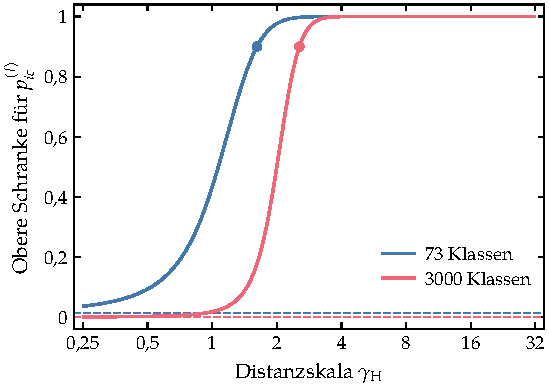
\includegraphics{neu/hoffer_skala}
  \caption[Wirkung der Distanzskala bei der Entropieminimierung nach Hoffer und Ailon]{Obere Schranke der Zuordnungswahrscheinlichkeit nach Gleichung~\eqref{eq:hoffer:schranke} über $\gamma_{\mathrm{H}}$ für 73 bzw.\ \num{3000} bekannte Klassen, etwa die Klassenzahlen eines Cars196- bzw.\ In-Shop-Folds bei Labels in jeder Klasse. Gestrichelt: Gleichverteilung $1/C_{\mathrm{L}}$. Punkte: notwendige Mindestskala für $p^{(l)}_{ic}=0{,}9$.}
  \label{fig:hoffer:skala}
\end{figure}

Die Entropieminimierung nach Hoffer und Ailon wird \ac{SERAPH} und \ac{ISMLP} vorgezogen, weil sie nur Embeddings und gelabelte Referenzbilder braucht und daher mit allen fünf Verlustfunktionen auf dieselbe Weise kombiniert werden kann. 

\ac{SERAPH} würde eine Auswahl ungelabelter Paare, eine Distanzschwelle und eine Übertragung der Spurregularisierung erfordern. Gegen \ac{SERAPH} spricht außerdem der Rechenaufwand, da das Verfahren nur langsam konvergiert~\cite{dutta_semi-supervised_2021} und eine Suche mit vielen Läufen damit teurer wird. \ac{ISMLP} benötigt Proxys, die, zumindest für paarbasierte Verlustfunktionen, zusätzlich ermittelt werden müssen. Beide Verfahren wurden in den Vorexperimenten erprobt (Abschnitt~\ref{sec:e:phase0}). Die Wahl begründet keine allgemeine Überlegenheit dieses Verfahrens. Ein einzelnes Referenzbild kann die Streuung einer Klasse nur eingeschränkt vertreten. Die Implementierung ist jedoch deutlich leichter und repräsentiert die Entropieminimierung ähnlich wie die anderen Verfahren. 

\subsection{\acs{SLADE}}
\label{sec:m:slade}
\ac{SLADE} wird als clusterbasierter Mechanismus umgesetzt. Alle $n_{\mathrm{T}}$ Epochen bettet der aktuelle Head die ungelabelten Bilder ein und teilt sie mit $k$-Means in so viele Cluster, wie es ein gesuchtes Verhältnis zur Zahl der gelabelten Klassen vorgibt. Bis zur nächsten Neuberechnung bleiben die Cluster fest. Basis $\bm{W}_a$, Verteilungsverlust (Gleichung~\eqref{eq:slade-sd}) und die Auswahl sicherer Paare folgen dem Originalverfahren~\cite{duan_slade_2021}. Die sicheren ungelabelten Paare gehen in dieselbe Verlustfunktion ein wie die gelabelten Bilder. Bei ArcFace und Proxy-Anchor ist das nicht möglich, weil deren Klassenparameter nur die gelabelten Klassen kennen und keine Paare aus unbekannten Clustern verarbeiten können (Abschnitt~\ref{sec:verluste:proxy}). Für diese beiden Verlustfunktionen gehen die sicheren Paare deshalb in einen Contrastive Loss nach Gleichung~\eqref{eq:contrastive} ein, wie in der ursprünglichen Arbeit, dessen Margen gesucht werden. Die Gewichte $w_{\mathrm{reg}}$ und $w_{\mathrm{basis}}$ aus Gleichung~\eqref{eq:slade} werden über eigene Zielverhältnisse $\eta$ und $\eta_{\mathrm{basis}}$ nach Abschnitt~\ref{sec:m:gewicht} bestimmt.

Im Original bildet ein eigens trainierter Teacher die Cluster, aus denen ein Student lernt, der den Teacher anschließend nach dem in Abschnitt~\ref{sec:ssdml} beschriebenen Schema ablöst~\cite{duan_slade_2021}. In dieser Arbeit wird kein getrennter Teacher verwendet. Die Cluster stammen vom selben linearen Head, der danach ohne Zurücksetzen der Gewichte oder des Optimierers weitertrainiert wird. Als Teacher dient nur der Head zum Zeitpunkt der letzten Neuberechnung und das Intervall $n_{\mathrm{T}}$ heißt in den Suchräumen deshalb Teacher-Aktualisierung (Anhang~\ref{sec:anhang:phase1}). Wie bei Noisy Student (Abschnitt~\ref{sec:teacher-student}) wird der Teacher damit periodisch durch den Student ersetzt~\cite{xie_self-training_2019}. Anders als dort wird dafür aber kein neues Modell trainiert. Bei $n_{\mathrm{T}}=1$ werden die Cluster wie die Pseudo-Labels von \ac{LP} und der Graph von \ac{LRML} in jeder Epoche aus den aktuellen Embeddings neu gebildet und vom Teacher-Student-Schema bleibt nur, dass die Ziele innerhalb einer Epoche fest sind.

Diese Umsetzung folgt aus dem Versuchsaufbau. Ein getrennter Teacher wäre wie der Student ein linearer Head auf denselben festen Merkmalen. Ein Self-Training aus mehreren vollständigen Trainingsläufen nacheinander würde zudem die Laufzeit vervielfachen. So berechnet \ac{SLADE} seine Ziele wie \ac{LP} und \ac{LRML} innerhalb eines einzigen Trainings aus dem aktuellen Head neu und bleibt mit ihnen vergleichbar. Mit dem Original teilt diese Variante die Idee, aus Clustern sichere Paarrelationen abzuleiten, nicht aber die Umsetzung als Self-Training. Die ursprüngliche Implementierung wird nicht übernommen, weil ein weitergereichter Teacher Labels aus vorherigen Folds gesehen hätte, die dann zur Validierung verwendet werden. Das wäre Leakage und würde die Validierungsleistung verzerren. 

\section{Training}
\label{sec:training}

Die Skalierung auf $224\times224$ Pixel erfolgt bilinear und ohne Zuschnitt. Nicht quadratische Bilder werden dadurch verzerrt, bleiben aber vollständig sichtbar.

Optimiert wird mit Adam ohne Weight Decay~\cite{kingma_adam_2015}. Verlustfunktionen mit eigenen Klassenparametern (Proxy-Anchor, ArcFace) erhalten einen eigenen Optimierer mit eigener, gesuchter Lernrate und beide Optimierer werden in jedem Schritt aktualisiert. In einer Epoche wird auf so vielen Trainingsbildern trainiert, wie der vollständige Trainingspool des Folds enthält, unabhängig vom Label-Budget. Dadurch ist die Zahl der Optimierungsschritte je Epoche für alle Budgets gleich.

Die \ac{SPC} beträgt 4 für Cars196 und \ac{CUB}, 2 für In-Shop und Semi-iNat-2021 und 8 für die In-Shop-Serie mit gelabelten Klassen. Die Werte sind je Datensatz fest und für alle Verlustfunktionen gleich. Es wird nur die Batchgröße gesucht. Eine größere \ac{SPC} ist auf In-Shop und Semi-iNat-2021 nicht möglich, weil beim kleinsten Budget $k=2$ jede Klasse nur zwei gelabelte Bilder hat. Auf Cars196 und \ac{CUB} beträgt das kleinste Budget $k=4$, sodass dort \ac{SPC}-4 möglich ist. Diesen Wert verwendet eine Vergleichsstudie bei Embedding Losses~\cite{musgrave_metric_2020}. Erst damit sind dort auch Batches mit 256 Bildern möglich, denn bei \ac{SPC}-2 wären dafür 128 Klassen nötig, beim Training stehen je Durchlauf der Kreuzvalidierung aber höchstens 80 Klassen zur Verfügung. Außerhalb ihrer Versuche zum Sampling (Abschnitt~\ref{sec:sampling}) wird in zwei weiteren Vergleichen für alle Verlustfunktionen ebenfalls eine einheitliche \ac{SPC} verwendet, \ac{SPC}-2~\cite{roth_revisiting_2020} bzw.\ \ac{SPC}-4~\cite{berton_all_2025, musgrave_metric_2020}.

Nach jeder Epoche wird auf dem vollständigen Validierungsfold ausgewertet. Behalten wird das Modell der Epoche mit der besten Validierungs-\ac{MAP@R}. Alle Angaben nach dem Training beziehen sich auf dieses Modell und nicht auf die letzte Epoche. Das Training endet, wenn sich die Validierungs-\ac{MAP@R} innerhalb der Patience (Abschnitt~\ref{sec:modellauswahl}) nicht verbessert. Die Patience ist für alle Verfahren gleich und beträgt auf Cars196, \ac{CUB} und In-Shop 20 Epochen und auf Semi-iNat-2021 zehn. Abweichend davon verwenden die Wiederholungen mit fünf Seeds auf \ac{CUB} für alle Verfahren eine Patience von 40 Epochen, weil ein Training dort wenig Rechenzeit benötigt. 





Für jeden Fold wird geprüft, ob die Patience das Training zu früh beendet, weil die Validierungs-\ac{MAP@R} nach einem anfänglichen Einbruch zu langsam wieder steigt. Jeder Lauf mit mindestens einem solchen Fold wird zusätzlich mit verzögerter Patience trainiert, bei der die ersten 20 Epochen nach dem Warm-up keine Patience verbrauchen. Damit alle Läufe eines Vergleichs gleich trainiert werden, berichtet die Arbeit für jeden Lauf die Variante ohne Verzögerung. Das Kriterium, die Ausnahmen und die Werte mit Verzögerung stehen in Anhang~\ref{chap:anhang:verzoegerung}.

\section{Ablauf der Untersuchung}
\label{sec:phasen}	

Der Untersuchung gehen explorative Vorexperimente voraus. In ihnen werden Verfahren und Varianten erprobt und an ihnen orientieren sich die Suchräume der anschließenden Hyperparameteroptimierung. Die Untersuchung selbst gliedert sich in zwei Phasen. Phase~1 bestimmt für jede Kombination die beste Konfiguration und wiederholt diese mit fünf Seeds über alle Budgets. Phase~2 untersucht mit gezielten Eingriffen und Analysen, worauf die Ergebnisse der Phase~1 beruhen.

\subsection{Vorexperimente}
\label{sec:m:phase0}


In den Vorexperimenten werden für die Kombinationen aus Datensatz, Mechanismus und Verlustfunktion 50 Konfigurationen zufällig gezogen und mit höchstens 500 Epochen trainiert. Mechanismen mit mehreren Varianten werden überwiegend in einer Basisvariante untersucht und daneben werden \ac{SERAPH} und \ac{ISMLP} als alternative entropiebasierte Verfahren getestet. In der Basiskonfiguration schließen die Bereiche für die Marge und die Skala von ArcFace, für die Parameter des \ac{MS} Loss mit Miner und für die Temperatur von \ac{NT-Xent} die Werte ein, die eine veröffentlichte Suche auf Cars196 und \ac{CUB} als beste ergab~\cite{musgrave_metric_2020}. Die Bereiche aller Verlustfunktionen enthalten zudem die Standardwerte der Bibliothek~\cite{musgrave_pytorch_losses_code_2026}. Für \ac{SLADE} ist der Bereich der Temperatur $\tau$ enger gefasst und schließt die in dieser Suche ermittelten Werte nicht ein, da der Gradient dort zu klein wird (Tabelle~\ref{tab:first-run-hyperparameter-spaces}). Von den dort aufgeführten Hyperparametern werden die beiden Lernraten, die Skalen $\gamma$ von ArcFace, Circle und Proxy-Anchor, $\gamma^{-}$ des \ac{MS} Loss und $\gamma_{\mathrm{H}}$ von Hoffer, die Temperatur $\tau$ von \ac{NT-Xent} und das Varianzgewicht $w_v$ von \ac{SLADE} logarithmisch gezogen, sodass jede Größenordnung gleich stark vertreten ist. Diese Wahl entspricht einer Empfehlung für Hyperparameter, die nur nach unten begrenzt sind~\cite{bischl_hyperparameter_2023}. 

Nach den Vorexperimenten werden die Grenzen der Suchräume anhand der Verteilung der Versuche über jeden Parameter angepasst. Dazu wird für jeden Versuch sein Rückstand auf den besten Versuch derselben Suche betrachtet. Als gut gilt ein Versuch, der bis auf einen Prozentpunkt an den besten heranreicht. Häufen sich gute Versuche an einer Grenze, könnte das Optimum außerhalb des Bereichs liegen und er wird in diese Richtung erweitert. Enthält ein Randbereich viele Versuche, aber kaum gute, wird er entfernt. Verteilen sich die guten Versuche über den ganzen Bereich, bleibt er unverändert. Für die Lernrate von Circle, \ac{MS} und \ac{NT-Xent} wird ein gemeinsamer niedriger Bereich gewählt, damit Unterschiede zwischen den drei paarbasierten Verlustfunktionen nicht auf verschiedene Suchräume der Lernrate zurückgehen. Das gilt auch für \ac{NT-Xent}, obwohl dort auch hohe Lernraten gute Versuche erreichen, denn der niedrige Bereich enthält für die \UEBL, \ac{LP} und \ac{LRML} ebenfalls gute Versuche, für Hoffer nicht (Abschnitt~\ref{sec:e:phase0}). Cars196 und In-Shop werden gemeinsam beurteilt, \ac{CUB} und Semi-iNat-2021 jeweils für sich. Die Grenzen beruhen damit auf einer Beurteilung der Verteilungen und nicht auf einer festen Regel.

\subsection{Phase 1: Hyperparameteroptimierung und Wiederholungen}
\label{sec:m:phase1}
Für jede Kombination sucht Phase~1 mit Optuna in 80 Versuchen. Zuerst werden 40 Konfigurationen zufällig gezogen, dann schlägt der \ac{TPE} 40 weitere vor~\cite{bergstra_algorithms_2011}. Verwendet wird die multivariate Variante aus Optuna~\cite{watanabe_tree-structured_2023}. Die 80 Versuche sind mehr als die 50 Iterationen bayesscher Optimierung in einer früheren Untersuchung~\cite{musgrave_metric_2020}, weil die \ac{SSL}-Mechanismen zusätzliche Hyperparameter haben. Die 40 zufälligen Versuche geben dem \ac{TPE} einen breiten Ausgangspunkt und dienen später als Stichprobe für die Sensitivitätsanalyse. Zielgröße ist die Validierungs-\ac{MAP@R}, gemittelt über die Folds. Die Versuche der Suche trainieren mit höchstens 600 Epochen, die Testevaluationen mit höchstens \num{1000}. Gesucht werden je nach Mechanismus 3 bis 17 Hyperparameter (Anhang~\ref{sec:anhang:phase1}). Bei \ac{LP} sind es 9 bis 12, bei \ac{SLADE} 13 bis 17 gegenüber 3 bis 6 bei der \UEBL (Tabelle~\ref{tab:phase1:hpo-protokoll}). Die beste Konfiguration wird unverändert auf alle Budgets übertragen und mit fünf Seeds wiederholt. Die Übertragung von einem Budget auf alle ist eine Vereinfachung. Ein Teil der Budgetabhängigkeit kann daraus entstehen, dass eine Konfiguration nur für $k=16$ (In-Shop: $k=2$) ausgewählt wurde und ein Mechanismus mit anderen Hyperparametern bei einem anderen Budget besser abschneiden könnte. 

\subsection{Phase 2: Ablationen}
\label{sec:m:phase2}

In Phase~2 wird untersucht, \emph{warum} ein Mechanismus hilft. Eine Erklärung gilt als gestützt, wenn eine gezielte Änderung des vermuteten Mechanismus die Retrieval-Leistung in die erwartete Richtung verschiebt. Eine Korrelation allein genügt nicht. Die Eingriffe und die erwarteten Richtungen wurden vor den Läufen festgelegt (Tabelle~\ref{tab:phase2:eingriffe} in Anhang~\ref{chap:anhang:phase2}).


Die Ablationen laufen auf Cars196 bei $k=16$ und $k=8$ sowie auf In-Shop bei $k=2$. Dabei ist $k=16$ das Budget der Hyperparametersuche, bei $k=8$ bleibt mehr Raum für Verbesserungen, weil die Mechanismen in Phase~1 dort mehr gewinnen als bei $k=16$. Jede Variante verwendet die Phase-1-Konfiguration mit Seed~2 und ändert nur die genannte Einstellung, sodass die Befunde für die Umgebung dieser Konfiguration gelten. Die Varianten laufen mit einer Grenze von \num{1000} Epochen. Da jede Variante je Budget nur einmal läuft, gilt ein Unterschied erst dann als Befund, wenn er deutlich größer ist als die Streuung zwischen zwei Seeds. Für zwei Läufe mit derselben Seed-Standardabweichung $\sigma$ aus den Phase-1-Wiederholungen beträgt die Standardabweichung ihrer Differenz bei vernachlässigter Kovarianz $\sqrt{2}\,\sigma$. Als Rauschschwelle dient das Doppelte davon, $2\sqrt{2}\,\sigma$, was bei unabhängigen, normalverteilten Läufen etwa einem zweiseitigen Niveau von \qty{5}{\percent} entspräche. Die tatsächliche Streuung der Differenz bestimmt diese Schwelle nicht, weil die Läufe ihren Seed teilen und die Varianz einer veränderten Variante nicht eigens geschätzt wird. Die Rauschschwelle dient der Einordnung, nicht einem kalibrierten Signifikanztest. Je nach Mechanismus und Verlustfunktion sind das 0,3 bis \num{1,1}~Prozentpunkte auf Cars196 bei $k=16$ und 0,1 bis \num{1,4}~Prozentpunkte auf In-Shop. Bei dem Vergleich mit der \UEBL tritt an die Stelle von $\sqrt{2}\,\sigma$ die Wurzel aus der Summe der Seed-Varianzen beider Konfigurationen, ebenfalls unter Vernachlässigung der Kovarianz. Wenn alle fünf Verlustfunktionen vorliegen, wird zusätzlich angegeben, ob ein Unterschied mit allen fünf dasselbe Vorzeichen hat. Eine solche einheitliche Richtung wird als Hinweis berichtet, auch wenn einzelne Unterschiede unter der Rauschschwelle bleiben. Als Befund gilt ein Unterschied aber nur für die Verlustfunktionen, bei denen er die Rauschschwelle übersteigt. Für die Concat-\ac{MAP@R} wird die Rauschschwelle auf dieselbe Weise aus der Seed-Standardabweichung der Concat-\ac{MAP@R} der Phase-1-Wiederholungen bestimmt. Bei $k=8$ stammen die Rauschschwellen aus den Phase-1-Wiederholungen bei $k=8$.

Neben der im Folgenden beschriebenen $2\times2$-Zerlegung, der Kontrolle mit abgeschaltetem \ac{SSL}-Term und den Oracle-Pseudo-Labels umfasst Phase~2 weitere Eingriffe. Pseudo-Labels bzw.\ Graph werden nach dem Warm-up einmal berechnet und danach nicht mehr erneuert. Der Graph von \ac{LP} und \ac{LRML} wird unter Erhalt der Knotengrade zufällig umverdrahtet~\cite{maslov_specificity_2002}. Mit den verdeckten Labels werden alle Kanten zwischen verschiedenen Klassen entfernt, als Kontrolle dieselbe Zahl zufälliger Kanten. Sweeps variieren je einen Hyperparameter der Phase-1-Konfiguration. Tabelle~\ref{tab:phase2:eingriffe} führt alle Eingriffe mit ihrer Umsetzung und der erwarteten Richtung auf.

Die $2\times2$-Zerlegung soll trennen, ob ein Gewinn von den ungelabelten Bildern oder von den eigens gesuchten Hyperparametern der \ac{SSL}-Konfiguration stammt. Sie kreuzt die Hyperparameter der \UEBL und die der \ac{SSL}-Konfiguration mit dem Training mit und ohne ungelabelte Bilder (Tabelle~\ref{tab:m:2x2}). Zwei der vier Kombinationen liegen bereits vor, die \UEBL selbst und die unveränderte \ac{SSL}-Konfiguration. Für die beiden übrigen wird jede \ac{SSL}-Konfiguration zweimal zusätzlich trainiert. Im ersten Lauf, der Variante mit den Hyperparametern der \UEBL, übernimmt sie für alle Hyperparameter, die beide Suchen optimiert haben, die Werte der \UEBL und behält nur ihre \ac{SSL}-spezifischen Parameter. Im zweiten Lauf, der Variante ohne ungelabelte Bilder, behält sie ihre eigenen Hyperparameter, aber ohne ungelabelte Bilder. Dazu erhält der ungelabelte Strom die gelabelten Bilder ohne ihre Labels, wobei die Zahl der Updates pro Epoche gleich bleibt. Mit den Hyperparametern der \UEBL ist der Lauf ohne ungelabelte Bilder dagegen die \UEBL selbst, in der Term und ungelabelte Bilder gemeinsam fehlen, sodass der Vergleich mit der \UEBL dort beide nicht trennt. In der Zeile der \ac{SSL}-Konfiguration zeigt der Vergleich also den Beitrag der ungelabelten Bilder, in der Spalte mit ungelabelten Bildern den der eigens gesuchten Hyperparameter.
\begin{table}[tbp]
  \centering
  \caption[Kombinationen der $2\times2$-Zerlegung]{Kombinationen der $2\times2$-Zerlegung. Ohne ungelabelte Bilder erhält der \acs{SSL}-Mechanismus statt der ungelabelten die gelabelten Bilder ohne ihre Labels.}
  \label{tab:m:2x2}
  \small\begin{tabular}{@{}l>{\raggedright\arraybackslash}p{5.0cm}>{\raggedright\arraybackslash}p{5.0cm}@{}}
    \toprule
    Hyperparameter & mit ungelabelten Bildern & ohne ungelabelte Bilder \\
    \midrule
    der \UEBL & Variante mit den Hyperparametern der \UEBL & \UEBL selbst \\
    der \acs{SSL}-Konfiguration & \acs{SSL}-Konfiguration aus Phase~1 & Variante ohne ungelabelte Bilder \\
    \bottomrule
  \end{tabular}
\end{table}
Den Beitrag des Terms allein zeigt der Vergleich der Variante ohne ungelabelte Bilder mit der Kontrolle mit abgeschaltetem \ac{SSL}-Term. Beide verwenden die \ac{SSL}-Hyperparameter, ihr Unterschied zeigt also, was der \ac{SSL}-Term bewirkt, wenn er nur die gelabelten Bilder sieht. Ohne vorab festgelegte Erwartung läuft jede \ac{SSL}-Konfiguration außerdem einmal ohne Warm-up.

Für \ac{LRML}, dessen Abstand zwischen Concat und Mean in Phase~1 auf Cars196 beim kleinsten Budget $k=4$ am weitesten über dem der \UEBL liegt, werden die $2\times2$-Zerlegung und die Kontrolle mit abgeschaltetem \ac{SSL}-Term außerdem bei $k=4$ mit allen fünf Verlustfunktionen und den fünf Seeds der Phase~1 trainiert. Dieser Versuch soll zeigen, welche Komponente den zusätzlichen Gewinn im Ensemble trägt. Die Unterschiede werden seedweise gepaart und es wird angegeben, in wie vielen der 25 Paare aus Verlustfunktion und Seed sie dasselbe Vorzeichen haben. Da die Embeddings jedes Heads auf Länge eins normiert werden, ist die Kosinusähnlichkeit zweier Bilder in $\bm{f}^{\mathrm{cat}}$ genau das Mittel ihrer Ähnlichkeiten in den vier Heads. Im Ensemble können sich deshalb nur Fehler wegmitteln, die nicht alle Heads teilen. Als Maß dafür dient der Anteil der falschen Nachbarn unter den ersten $R_q$ Treffern eines Heads, die ein anderer Head für dieselbe Query ebenfalls unter seinen ersten $R_q$ Treffern hat. Gemittelt wird über alle Paare von Heads und jede siebte Query der Testmenge.

In der In-Shop-Serie mit gelabelten Klassen läuft die $2\times2$-Zerlegung für \ac{LRML} außerdem bei \qty{10}{\percent} gelabelter Klassen, dem Anteil der Hyperparametersuche, mit allen fünf Verlustfunktionen und Seed~2. Die ungelabelten Bilder stammen dort ausschließlich aus Klassen ohne Label. Die Variante ohne ungelabelte Bilder zeigt deshalb, ob \ac{LRML} Bilder neuer Klassen verwerten kann. Die Rauschschwellen stammen hier aus den Phase-1-Wiederholungen bei \qty{10}{\percent}.

Die Oracle-Varianten berechnen in jeder Epoche die Pseudo-Labels und die Auswahl der übernommenen Bilder aus ihrem jeweils aktuellen Head. Für die ausgewählten Bilder ersetzen sie die Pseudo-Labels durch die wahren Labels. Eine je Bild fest gezogene Zufallszahl bestimmt, ob sein Label bei einer vorgegebenen Fehlerrate von 0, 10, 20, 40 bzw.\ \qty{60}{\percent} verfälscht wird. Die so entstehende Kurve zeigt, ob reguläres \ac{LP} bei gleicher gemessener Fehlerrate über oder unter den Läufen mit zufälligen Fehlern liegt. Verrauschte Labels wurden auch beim Training von Retrieval-Modellen untersucht, dort aber an den gelabelten Trainingsdaten und nicht an Pseudo-Labels~\cite{berton_all_2025}.

Dabei wurde auf Cars196 und \ac{CUB} auch bei \qty{32}{\percent} zufällig verfälschten Labels eine geringe Rauschempfindlichkeit berichtet~\cite{berton_all_2025}.

\subsection{Externe ungelabelte Bilder}
\label{sec:m:extern}

\ac{SLADE} wurde in einem anderen Setting evaluiert als dem dieser Arbeit. Dort sind alle Bilder der Trainingsklassen gelabelt und die ungelabelten Bilder stammen aus einem externen Datensatz~\cite{duan_slade_2021}. Ein zusätzlicher Versuch überträgt dieses Setting auf alle vier Mechanismen. Auf Cars196 und In-Shop sind alle Bilder der Trainingsklassen gelabelt. Der ungelabelte Pool besteht aus einem Anteil von CompCars bzw.\ Fashion200k (Abschnitt~\ref{sec:daten}). Auf Cars196 werden 10, 25, 50 und \SI{100}{\percent} der \num{16537} Bilder verwendet, auf In-Shop 5, 10, 25 und \SI{50}{\percent} der \num{338340} Bilder. Die Auswahl ist fest, für alle Folds und Mechanismen gleich und geschachtelt, sodass ein größerer Anteil die Bilder jedes kleineren enthält. Bei CompCars verteilt sie sich gleichmäßig über dessen Klassen. Jeder Mechanismus läuft mit allen fünf Verlustfunktionen, Seed~2 und seiner Phase-1-Konfiguration mit höchstens \num{1000} Epochen. Die Hyperparameter wurden also für wenige Labels und den internen Pool gesucht und für dieses Setting nicht neu optimiert. Referenz ist die \UEBL mit allen Labels, ebenfalls mit Seed~2 und ihrer Phase-1-Konfiguration. Als Kontrolle läuft jede \ac{SSL}-Konfiguration außerdem mit allen Labels und ohne externe Bilder. \ac{LP} und \ac{LRML} erhalten dann einen leeren ungelabelten Pool, sodass \ac{LP} keine Pseudo-Labels bildet und der Term von \ac{LRML} nur auf dem Graphen der gelabelten Bilder wirkt. Hoffer und \ac{SLADE} benötigen ungelabelte Bilder und laufen deshalb mit abgeschaltetem \ac{SSL}-Term. Auf Cars196 laufen \ac{LP} und \ac{LRML} zusätzlich bei jedem Anteil mit 50, 100, 200 und 300 Nachbarn und \ac{SLADE} mit einer festen Zahl von 100 bis 500 Clustern statt des Clusterverhältnisses, im Bereich der Clusterzahlen, die für \ac{SLADE} untersucht wurden~\cite{duan_slade_2021}. Ein Unterschied gilt wie in Phase~2 erst oberhalb der Rauschschwelle für den Vergleich mit der \UEBL als Befund (Abschnitt~\ref{sec:m:phase2}).

\subsection{Verfolgung der Embedding-Geometrie}
\label{sec:m:geometrie}
Um zu erkennen, wie die Mechanismen den Embedding-Raum verändern, werden die Phase-1-Konfigurationen\footnote{Für \ac{LRML} verwenden die Geometrieläufe auf Cars196, In-Shop und in der In-Shop-Serie mit gelabelten Klassen die Konfiguration einer Suche, die sich von der in Abschnitt~\ref{sec:m:phase1} nur durch die univariate Variante des \ac{TPE} unterscheidet.} mit Seed~2 für alle 25 Kombinationen trainiert und dabei verfolgt. Auf Cars196 und Semi-iNat-2021 werden alle vier Budgets betrachtet, auf In-Shop $k=2$ und 4. In der In-Shop-Serie mit gelabelten Klassen werden alle vier Anteile betrachtet. Die Geometrieläufe berechnen die Maße aus Abschnitt~\ref{sec:geometrie} nach jeder Epoche auf allen Bildern. Auf Cars196 und auf Semi-iNat-2021 bei $k=16$ wird dieselbe Konfiguration zusätzlich in getrennten Graphläufen trainiert. Die Graphläufe halten für eine feste Auswahl von 4000 Bildern des Trainingspools die Embeddings und den \ac{kNN}-Graphen fest und speichern die Pseudo-Labels, die \ac{LP} in jeder Epoche übernimmt. Darauf beruhen die Darstellung mit \ac{t-SNE} und die Auswertung der Pseudo-Labels in Abschnitt~\ref{sec:e:pseudolabels}.

Die Maße werden in den Geometrieläufen vor dem ersten Optimierungsschritt (Epoche~$-1$) und danach nach jeder Epoche getrennt für den ganzen Trainingspool, seine gelabelten und seine ungelabelten Bilder, die Validierungs- und die Testklassen berechnet. In den Graphläufen erfolgt die Messung dagegen nur nach jeder fünften Epoche, auf Semi-iNat-2021 nach jeder zweiten. So lässt sich unterscheiden, ob ein Head nur die gelabelten Bilder ordnet oder auch die übrigen Bilder derselben Klassen und ungesehene Klassen. Spektraler Abfall und $\pi_{\mathrm{ratio}}$ werden aus der Referenzimplementierung übernommen~\cite{roth_revisiting_code_2020}. $\pi_{\mathrm{intra}}$, $\pi_{\mathrm{inter}}$ und ihr Verhältnis werden in jeder gemessenen Bildmenge nur über die Klassen berechnet, die dort mindestens zwei Bilder haben, damit das Verhältnis für beide Maße dieselben Klassen beschreibt. $\pi_{\mathrm{inter}}$ und das Verhältnis setzen zusätzlich mindestens zwei dieser Klassen voraus. Bezugspunkt ist neben den DINOv2-Merkmalen der Head vor dem ersten Optimierungsschritt, weil schon die zufällige Projektion das Spektrum verändern kann.

Mit den verdeckten Labels werden außerdem zwei Größen gemessen. Als Prototyp einer Klasse dient der Mittelpunkt der Embeddings ihrer gelabelten Bilder~\cite{snell_prototypical_2017}. Anders als dort, wo der nächste Prototyp nach der quadrierten euklidischen Distanz bestimmt wird, entscheidet hier die Kosinusähnlichkeit. Die Genauigkeit der Prototypen-Zuordnung ist der Anteil der ungelabelten Bilder, deren ähnlichster Prototyp zu ihrer eigenen Klasse gehört. Die Reinheit der Kanten ist der Anteil der Kanten eines \ac{kNN}-Graphen über den Trainingspool zwischen Bildern derselben Klasse. Die Prototypen-Genauigkeit ist für die In-Shop-Serie mit gelabelten Klassen nicht definiert, da die ungelabelten Bilder dort zu Klassen ohne gelabeltes Bild gehören. Die Reinheit wird mit der Nachbarzahl und der Gewichtung des jeweiligen Mechanismus gemessen und für die \UEBL, Hoffer und \ac{SLADE} mit zehn Nachbarn. Sie ist daher nur bei gleicher Graphkonstruktion unmittelbar vergleichbar. 

Für die falschen Pseudo-Labels von \ac{LP} wird gezählt, wie viele ein Modell desselben Herstellers nennen, verglichen mit dem Anteil bei zufälliger Verwechslung. Diese Auswertung beruht auf den tatsächlich im Training übernommenen Pseudo-Labels des ganzen Pools, nicht auf der zusätzlichen Propagation der Graphläufe. Die verfolgten Bilder des Graphlaufs auf Cars196 werden mit \ac{t-SNE} dargestellt~\cite{van_der_maaten_visualizing_2008}. Die Maße nach dem Training stammen in den Geometrieläufen aus der per Validierung gewählten Epoche, in den Graphläufen aus der letzten verfolgten Epoche, die nicht nach ihr liegt. Die Tabellen und die Abbildungen mitteln über die Verlustfunktionen und die vier Folds. Verhältnisse werden dabei je Fold berechnet und erst danach gemittelt, sodass ein Tabellenmittel des Verhältnisses nicht dem Verhältnis der Tabellenmittel entsprechen muss.%


Vorab wurde folgende Erwartung festgelegt: Wenn die ungelabelten Bilder als Regularisierer gegen die Überanpassung an wenige Labels wirken, sollte der Head der \UEBL bei kleinem $k$ stärker komprimieren als die Heads der \ac{SSL}-Mechanismen, erkennbar an einem größeren spektralen Abfall. Der Unterschied sollte mit wachsendem $k$ kleiner werden. Zusätzlich prüft die Arbeit, ob sich der in Abschnitt~\ref{sec:geometrie} beschriebene Zusammenhang zwischen den Geometriemaßen und der Leistung auf ungesehenen Klassen in diesem Setting wiederfindet. Dazu werden die Maße nach dem Training für jede Kombination aus Verfahren, Verlustfunktion und Budget über die vier Folds gemittelt. Die Korrelation mit der Test-\ac{MAP@R} der einzelnen Fold-Modelle wird über alle Kombinationen eines Datensatzes bzw. einer In-Shop-Serie und innerhalb jedes Budgets berechnet. Grundlage dafür ist, wie im ursprünglichen Vorgehen~\cite{roth_revisiting_2020}, der Trainingspool. Weil die ungelabelten Bilder des Pools für die \ac{SSL}-Mechanismen aber Trainingsdaten sind und für die \UEBL nicht, wird die Korrelation zusätzlich auf den Validierungs- und den Testklassen berechnet, deren Bilder in keinen Gradientenschritt eingehen.


\subsection{Sensitivitätsanalyse der Hyperparameter}
\label{sec:m:sensitivitaet}

Zusätzlich werden die vorhandenen Versuche der
Vorexperimente und der Phase~1 ausgewertet, ohne neue
Läufe durchzuführen. Für die zufällig gezogenen
Konfigurationen der Phase~1 (Abschnitt~\ref{sec:modellauswahl}) wird für jeden numerischen
Hyperparameter die Rangkorrelation nach Spearman mit
der Validierungs-\ac{MAP@R} bestimmt~\cite{spearman_proof_1904}.
In dieser Arbeit hebt sich ein Hyperparameter in einer Suche vom Rauschen ab, wenn diese
Rangkorrelation zweiseitig auf dem Niveau von \qty{5}{\percent} von null verschieden ist.

Als deskriptives Maß für die Häufigkeit nahezu
optimaler Konfigurationen werden die Anzahl und der
Anteil der Versuche bestimmt, deren Validierungs-\ac{MAP@R}
höchstens einen Prozentpunkt beziehungsweise einen
Standardfehler der Fold-Werte unter dem besten
Ergebnis liegt.

\subsection{Messung von Rechenzeit und Speicherbedarf}
\label{sec:m:aufwand}

Die Läufe der Hyperparametersuche und der Wiederholungen liefen parallel und bei wechselnder Auslastung auf geteilten \acp{GPU}, sodass ihre Laufzeiten nicht vergleichbar sind. Stattdessen wird auf In-Shop bei $k=2$ für jede Kombination aus Verfahren und Verlustfunktion die in Phase~1 gewählte Konfiguration mit einer Batchgröße von 128 für einen Fold allein auf einer H100-\ac{GPU} trainiert, bei \ac{LRML} eine Konfiguration aus einer anderen Suche mit derselben Verlustfunktion. Gemessen werden nach dem Warm-up die mittlere Dauer eines Trainingsschritts und die mittlere Dauer einer Epoche, einschließlich der Neuberechnung des Graphen, der Pseudo-Labels oder der Cluster und der Validierung. Berichtet wird der Median über die fünf Verlustfunktionen. Die Dauer eines Folds ergibt sich aus den Raten, die bei der Batchgröße des jeweiligen Phase-1-Folds gemessen wurden (Batchgrößen 32 bis 512), dessen Warm-up und der Zahl seiner trainierten Epochen. Berichtet wird der Median über die 100 Folds je Verfahren aus fünf Verlustfunktionen, fünf Seeds und vier Folds.

Der Speicherbedarf der Verlustfunktionen hängt nicht vom Bildinhalt ab und wird deshalb mit zufälligen Merkmalen bestimmt. Gemessen wird der Spitzenwert des zusätzlich belegten \ac{GPU}-Speichers gegenüber dem Zustand vor einem Trainingsschritt.

\chapter{Ergebnisse}
\label{chap:ergebnisse}

\newcommand{\CarsStat}[1]{\csname cars-stat-#1\endcsname}
\expandafter\def\csname cars-stat-vt-cells\endcsname{80}
\expandafter\def\csname cars-stat-vt-larger\endcsname{63}
\expandafter\def\csname cars-stat-vt-dv\endcsname{$2{,}76$}
\expandafter\def\csname cars-stat-vt-dt\endcsname{$1{,}81$}


Das Kapitel folgt dem Ablauf der Untersuchung. Differenzen werden in Prozentpunkten angegeben, Streuungen, wo nicht anders angegeben, als Standardabweichung über die fünf Seeds. \UEBL bezeichnet die supervised Referenz mit derselben Verlustfunktion wie das jeweils verglichene Verfahren.

\section{Suchräume und Auswahl der Verfahren}
\label{sec:e:phase0}

Die Vorexperimente veränderten vor allem die Bereiche der Skalen und der Lernrate. Der Bereich der ArcFace-Skala wurde verschoben, die Temperatur von \ac{NT-Xent} eingeengt und die Skala $\gamma^{-}$ des \ac{MS} Loss erweitert. Für Circle, \ac{MS} und \ac{NT-Xent} wurde die Lernrate auf $[10^{-5},5\cdot10^{-4}]$ begrenzt, bei ArcFace und Proxy-Anchor blieb der breite Bereich $[10^{-5},10]$ bestehen. Das gilt für Cars196, In-Shop und die In-Shop-Serie. Auf \ac{CUB} liegt der Bereich von Circle, \ac{MS} und \ac{NT-Xent} bei $[5\cdot10^{-6},10^{-4}]$, auf Semi-iNat-2021 der aller fünf Verlustfunktionen. \ac{SLADE} begrenzt die Lernrate mit allen fünf Verlustfunktionen (Tabelle~\ref{tab:hyperparameter-spaces}). Bei \ac{NT-Xent} lagen allerdings in den Suchen der \UEBL, von \ac{LP}, \ac{LRML} und Hoffer auf Cars196 und In-Shop die meisten guten Versuche über $5\cdot10^{-4}$, bei Circle und \ac{MS} nur rund ein Viertel. In sechs dieser acht Suchen lag bei \ac{NT-Xent} aber auch unterhalb der Grenze ein guter Versuch. In Phase~1 liegt die gewählte Lernrate von \ac{NT-Xent} nur in zwei der 25 Suchen nahe der oberen Grenze ihres Bereichs, mit \ac{LRML} auf Cars196 und auf Semi-iNat-2021, in den übrigen deutlich darunter. Alle Suchräume stehen in Anhang~\ref{chap:anhang:suchraeume}. In den Vorexperimenten erreichte die hier umgesetzte Fassung von \ac{SERAPH} auf Cars196 das Niveau der \UEBL und wurde nicht weiter verfolgt. Die Fassung von \ac{ISMLP} lag auf Cars196 gleichauf mit \ac{LRML} und Hoffer, auf In-Shop aber unter ihnen und brachte damit gegenüber Hoffer keinen Vorteil, der die zusätzlichen Proxys und die zusätzlichen Optimierungsschritte gerechtfertigt hätte. Beide Befunde beruhen auf zufälligen Suchen mit je 50 Versuchen und gelten für diese Umsetzungen, nicht für die Verfahren allgemein.%


\section{Leistung ohne ungelabelte Bilder}
\label{sec:e:ausgangslage}

Tabelle~\ref{tab:e:referenz} zeigt die Leistung der unveränderten DINOv2-Merkmale und der supervised Referenz \UEBL. Schon der zufällig initialisierte Head vor dem ersten Optimierungsschritt senkt die Ausgangsleistung, auf Cars196 und In-Shop um weniger als einen halben Prozentpunkt, auf \ac{CUB} und Semi-iNat-2021 um fast einen Prozentpunkt.%


\begin{table}[tbp]
\centering\small\setlength{\tabcolsep}{4pt}
\caption[Ausgangsleistung und supervised Referenz]{Test-MAP@R (Mean, Concat) der unveränderten DINOv2-Merkmale und der \UEBL in \%, bei der \UEBL Mittel $\pm$ Standardabweichung der 25 Läufe aus fünf Verlustfunktionen und fünf Seeds, die vor allem die Unterschiede zwischen den Verlustfunktionen wiedergibt. Alle Labels: alle Bilder der Trainingsklassen gelabelt, auf Cars196 und In-Shop nur Seed~2 (fünf Läufe).}
\label{tab:e:referenz}
\begin{tabular}{@{}l S[table-format=2.1] *{5}{S[table-format=2.1(2), retain-zero-uncertainty]}@{}}
\toprule
 & {DINOv2} & \multicolumn{4}{c}{\UEBL je Label-Budget} & {\UEBL, alle Labels} \\
\midrule
\textbf{Cars196} & & {$k=4$} & {$k=8$} & {$k=16$} & {$k=32$} & \\
\quad Mean & 20.3 & 32.6 +- 0.9 & 37.2 +- 0.8 & 40.1 +- 0.8 & 41.7 +- 0.8 & 43.1 +- 1.0 \\
\quad Concat & 20.3 & 34.9 +- 0.9 & 40.4 +- 0.8 & 43.5 +- 0.7 & 44.8 +- 0.6 & 45.3 +- 0.8 \\
\midrule
\textbf{\acs{CUB}} & & {$k=4$} & {$k=8$} & {$k=16$} & {$k=32$} & \\
\quad Mean & 52.4 & 51.7 +- 0.2 & 52.0 +- 0.2 & 52.1 +- 0.2 & 52.2 +- 0.3 & 52.3 +- 0.3 \\
\quad Concat & 52.4 & 52.2 +- 0.2 & 52.6 +- 0.3 & 52.9 +- 0.3 & 53.0 +- 0.3 & 53.1 +- 0.3 \\
\midrule
\textbf{Semi-iNat-2021} & & {$k=2$} & {$k=4$} & {$k=16$} & {$k=100$} & \\
\quad Mean & 34.0 & 34.1 +- 0.1 & 34.7 +- 0.1 & 36.0 +- 0.2 & 37.1 +- 0.3 & 37.1 +- 0.3 \\
\quad Concat & 34.0 & 34.6 +- 0.1 & 35.4 +- 0.1 & 37.0 +- 0.1 & 37.8 +- 0.2 & 37.9 +- 0.3 \\
\midrule
\textbf{In-Shop} & & {$k=2$} & {$k=4$} &  &  & \\
\quad Mean & 13.7 & 54.6 +- 0.7 & 59.2 +- 1.2 &  &  & 60.1 +- 1.6 \\
\quad Concat & 13.7 & 57.4 +- 0.9 & 60.4 +- 1.2 &  &  & 60.9 +- 1.6 \\
\bottomrule
\end{tabular}
\end{table}


Wie viel ein Training bewirkt, hängt stark vom Datensatz ab. Auf Cars196 ist der erste Treffer der DINOv2-Merkmale meist ein Auto desselben Modells (\ac{P@1} \qty{78.2}{\percent}), die übrigen Bilder der Klasse stehen aber verstreut im Ranking (\ac{MAP@R} \qty{20.3}{\percent}). Schon mit vier gelabelten Bildern je Klasse hebt die \UEBL die Mean-\ac{MAP@R} auf \qty{32.6}{\percent}. Auf In-Shop ist der Sprung noch größer. Die \UEBL steigt dort bereits bei $k=2$ von \qty{13.7}{\percent} auf \qty{54.6}{\percent}. Mit allen Labels der Trainingsklassen liegt die \UEBL mit Seed~2 auf Cars196 \num{1.8} und auf In-Shop \num{0.8} Prozentpunkte über dem Wert desselben Seeds beim größten Budget.%



Auf \ac{CUB} ist es umgekehrt. Die unveränderten Merkmale erreichen bereits eine \ac{MAP@R} von \qty{52.4}{\percent} und die \UEBL liegt als Einzelmodell bei jedem Budget darunter (Tabelle~\ref{tab:e:referenz}). Das gilt für die meisten trainierten Einzelmodelle, in 84 der 100 Kombinationen aus Verfahren, Verlustfunktion und Budget. Gegenüber dem zufällig initialisierten Head verbessert die \UEBL die Leistung zwar bei jedem Budget, holt den Verlust durch die Projektion aber nicht ganz auf und keine trainierte Konfiguration erreicht die \ac{P@1} der Merkmale von \qty{87.6}{\percent}. Erst die Ensembles übertreffen die Merkmale, in 93 der 100 Kombinationen und um höchstens \num{1.3} Prozentpunkte. Selbst mit allen Labels der Trainingsklassen erreicht die \UEBL als Einzelmodell nur das Niveau der Merkmale.%




Semi-iNat-2021 liegt näher an \ac{CUB} als an Cars196. Die \UEBL liegt bei $k=2$ als Einzelmodell nur knapp über den unveränderten Merkmalen und gewinnt bis $k=100$ nur rund drei Prozentpunkte hinzu, mit allen Labels kaum mehr (Tabelle~\ref{tab:e:referenz}). Anders als auf \ac{CUB} holt das Training den Verlust der zufälligen Projektion schon bei $k=2$ auf.%

Auf \ac{CUB} liegt schon die Validierung vor dem Training hoch. Ein Validierungsfold umfasst dort rund 20 Klassen und der zufällig initialisierte Head erreicht im Mittel je nach Fold eine Validierungs-\ac{MAP@R} von \qty{72.5}{\percent} bis \qty{86.3}{\percent} und eine \ac{P@1} von \qty{92.5}{\percent} bis \qty{99.5}{\percent}. Die \UEBL hebt die Validierungs-\ac{MAP@R} im Mittel je nach Budget nur um \num{1.4} bis \num{2.8} Prozentpunkte, die gewählte Epoche liegt im Median bei 5 bis 17. Die Auswahl bleibt trotzdem messbar, denn zwischen den 100 Kombinationen liegen in der Validierung \num{2.5} und im Test \num{2.4} Prozentpunkte, während die Seeds einer Kombination im Median nur um \num{0.15} bzw.\ \num{0.13} Prozentpunkte streuen.


\section{Nutzen ungelabelter Bilder}
\label{sec:e:phase1}

 Abbildung~\ref{fig:e:gewinne} fasst die gepaarten Gewinne gegenüber der \UEBL, gemittelt über die fünf Verlustfunktionen, zusammen. Anhang~\ref{chap:anhang:ergebnisse} enthält die Einzelheiten dazu, die Gewinne mit ihrer Standardabweichung (Tabelle~\ref{tab:anhang:gewinne}), ihren Verlauf über das Budget mit der Spanne über die Verlustfunktionen (Abbildung~\ref{fig:e:uebersicht}), die Werte je Verlustfunktion und die Zahl der Vergleiche mit negativer Differenz (Tabelle~\ref{tab:anhang:negativ}).

\begin{figure}[tbp]
  \centering
  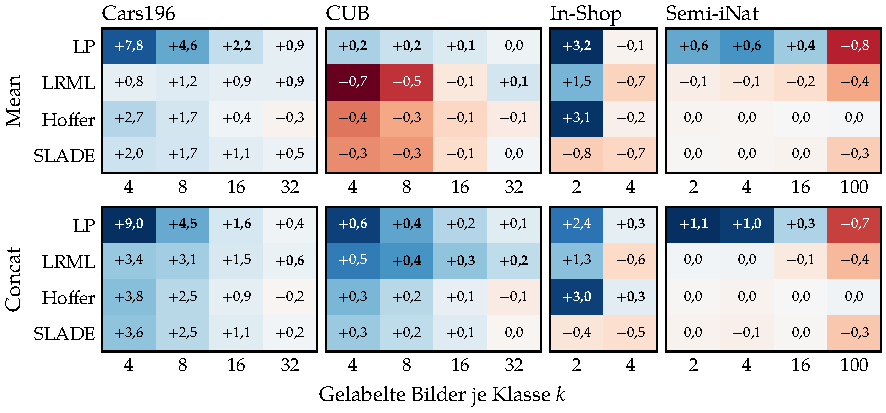
\includegraphics{neu/phase1_gewinne}
  \caption[Gewinn der \acs{SSL}-Verfahren gegenüber der supervised Referenz]{Gepaarter Gewinn der Test-\acs{MAP@R} der vier \acs{SSL}-Verfahren gegenüber der \UEBL in Prozentpunkten, gemittelt über die fünf Seeds und die fünf Verlustfunktionen. Fett: größter gerundeter Gewinn je Datensatz und Budget, getrennt nach Mean und Concat, sofern er positiv ist. Farbskala je Datensatz symmetrisch um null.}
  \label{fig:e:gewinne}
\end{figure}

\subsection{Cars196}

Auf Cars196 gewinnen bei kleinen Budgets alle vier Mechanismen gegenüber der \UEBL, \ac{LP} am meisten (Abbildung~\ref{fig:e:gewinne}). Bei $k=4$ gewinnt \ac{LP} als Einzelmodell im Mittel \num{7.8} Prozentpunkte, wie bei $k=8$ und $k=16$ ohne einen einzigen negativen Vergleich. Mit vier gelabelten Bildern je Klasse erreicht es das Niveau der Referenz mit 16, mit acht das der Referenz mit 32. Hoffer und \ac{SLADE} gewinnen bei $k=4$ deutlich weniger. \ac{LRML} verbessert das Einzelmodell nur wenig, das Ensemble aber um \num{3.4} Prozentpunkte. Dieser Unterschied zwischen dem Einzelmodell und dem Ensemble wird in Abschnitt~\ref{sec:e:faktoren} genauer betrachtet.%


\subsection{\acs{CUB}}

Auf \ac{CUB} bleiben alle mittleren Unterschiede unter einem Prozentpunkt (Abbildung~\ref{fig:e:gewinne}). Als Einzelmodelle liegen \ac{LRML}, Hoffer und \ac{SLADE} bis $k=16$ im Mittel sogar unter der \UEBL, im Ensemble gewinnen alle vier Verfahren wenige Zehntel eines Prozentpunkts. Die Mechanismen verändern auf \ac{CUB} also vor allem wenig und die Einzelmodelle bleiben meist unter den unveränderten Merkmalen (Abschnitt~\ref{sec:e:ausgangslage}).%


\subsection{In-Shop}

Auf In-Shop gewinnen bei $k=2$ \ac{LP} und Hoffer am meisten, je gut drei Prozentpunkte als Einzelmodell und in allen 25 Vergleichen (Abbildung~\ref{fig:e:gewinne}, Tabelle~\ref{tab:anhang:negativ}). \ac{LRML} gewinnt etwa halb so viel, \ac{SLADE} ist im Mittel schlechter als die \UEBL. Bei $k=4$, wenn bereits \qty{60}{\percent} des Trainingspools gelabelt sind, verschwindet der Gewinn bei allen Verfahren. Obwohl die DINOv2-Merkmale auf In-Shop ohne Training viel schwächer sind als auf Cars196, fällt der größte Gewinn kleiner aus.%


\subsection{Semi-iNat-2021}

Auf Semi-iNat-2021 hilft nur \ac{LP} (Abbildung~\ref{fig:e:gewinne}). Bis $k=16$ ist \ac{LP} in jedem gepaarten Vergleich besser als die \UEBL, bei $k=2$ um \num{0.6} Prozentpunkte als Einzelmodell. Mit zwei Labels je Art erreicht \ac{LP} das Niveau der Referenz mit vier. Bei $k=100$ kehrt sich der Gewinn in einen Verlust um. \ac{LRML}, Hoffer und \ac{SLADE} bleiben bei allen Budgets im Mittel über die Verlustfunktionen innerhalb eines halben Prozentpunkts um die \UEBL.%


Trotz des geringen Unterschieds zwischen der Leistung der \UEBL und der von \ac{LP} ist der Gewinn von \ac{LP} kein Zufall der Seeds, denn die Standardabweichung über die Seeds beträgt je Konfiguration höchstens \num{0.11} Prozentpunkte. Die Werte je Verlustfunktion stehen in Tabelle~\ref{tab:anhang:semiinat}. 

Zusammengefasst helfen ungelabelte Bilder vor allem auf Cars196 und auf In-Shop bei wenigen Labels, kaum auf \ac{CUB} und Semi-iNat-2021, wo auch zusätzliche echte Labels vergleichsweise wenig bringen (Abschnitt~\ref{sec:e:ausgangslage}). \ac{LP} gewinnt beim kleinsten Budget auf Cars196, In-Shop und Semi-iNat-2021 in jedem gepaarten Vergleich.%




\section{Einflussfaktoren}
\label{sec:e:faktoren}

\subsection{Label-Budget, Verfahren und Verlustfunktion}
\label{sec:e:beste}

Liegt ein Verfahren beim kleinsten Budget im Mittel über der \UEBL, ist sein Gewinn beim größten Budget auf allen vier Datensätzen kleiner, als Einzelmodell wie im Ensemble (Abbildung~\ref{fig:e:gewinne}). Einzige Ausnahme ist \ac{LRML} als Einzelmodell auf Cars196, dessen Gewinn bei allen Budgets zwischen \num{0.8} und \num{1.2} Prozentpunkten liegt. Am stärksten sinkt der Gewinn von \ac{LP} auf Cars196. Von $k=4$ bis $k=32$ fällt er als Einzelmodell von \num{7.8} auf \num{0.9} Prozentpunkte und im Ensemble um \qty{96}{\percent}, während der ungelabelte Pool um \qty{36}{\percent} schrumpft und die \UEBL im Ensemble um rund zehn Prozentpunkte zulegt.%

\begin{table}[tbp]
\centering\small\setlength{\tabcolsep}{4pt}
\caption[Beste Kombination aus Verfahren und Verlustfunktion]{Höchste Test-MAP@R in \% je Datensatz, Budget und Modelltyp, Mittel über die fünf Seeds. \acs{SSL}: beste der 20 Kombinationen aus den vier \acs{SSL}-Mechanismen und den fünf Verlustfunktionen (Spalten Verfahren und Verlust), \UEBL: mit der besten der fünf Verlustfunktionen.}
\label{tab:e:beste}
\begin{tabular}{@{}l *{2}{l l S[table-format=2.1] S[table-format=2.1]}@{}}
\toprule
 & \multicolumn{4}{c}{Einzelmodell (Mean)} & \multicolumn{4}{c}{Ensemble (Concat)} \\
\cmidrule(lr){2-5}\cmidrule(l){6-9}
Budget & Verfahren & Verlust & {\acs{SSL}} & {\UEBL} & Verfahren & Verlust & {\acs{SSL}} & {\UEBL} \\
\midrule
\multicolumn{9}{@{}l}{\textbf{Cars196}} \\
\quad $k=4$ & \acs{LP} & \acs{MS} & 41.5 & 34.3 & \acs{LP} & \acs{MS} & 45.6 & 36.5 \\
\quad $k=8$ & \acs{LP} & \acs{MS} & 42.6 & 38.6 & \acs{LP} & \acs{MS} & 46.1 & 41.6 \\
\quad $k=16$ & \acs{LP} & \acs{MS} & 43.3 & 41.3 & \acs{LP} & \acs{MS} & 46.3 & 44.5 \\
\quad $k=32$ & \acs{LP} & \acs{MS} & 43.4 & 43.0 & \acs{LP} & \acs{MS} & 46.4 & 45.9 \\
\midrule
\multicolumn{9}{@{}l}{\textbf{\acs{CUB}}} \\
\quad $k=4$ & \acs{LP} & \acs{MS} & 52.4 & 51.8 & \acs{LP} & \acs{MS} & 53.3 & 52.5 \\
\quad $k=8$ & \acs{LP} & \acs{MS} & 52.7 & 52.1 & \acs{LP} & \acs{MS} & 53.4 & 52.9 \\
\quad $k=16$ & \acs{LP} & \acs{MS} & 52.8 & 52.4 & \acs{LP} & \acs{MS} & 53.5 & 53.2 \\
\quad $k=32$ & \acs{LP} & \acs{MS} & 52.9 & 52.7 & \acs{LP} & \acs{MS} & 53.7 & 53.5 \\
\midrule
\multicolumn{9}{@{}l}{\textbf{In-Shop}} \\
\quad $k=2$ & \acs{LP} & ArcFace & 58.9 & 55.9 & \acs{LP} & \acs{MS} & 61.1 & 58.8 \\
\quad $k=4$ & \acs{LP} & \acs{MS} & 60.4 & 60.6 & \acs{LP} & \acs{MS} & 62.2 & 61.6 \\
\midrule
\multicolumn{9}{@{}l}{\textbf{Semi-iNat-2021}} \\
\quad $k=2$ & \acs{LP} & \acs{MS} & 35.1 & 34.1 & \acs{LP} & \acs{MS} & 35.9 & 34.6 \\
\quad $k=4$ & \acs{LP} & \acs{MS} & 35.8 & 34.8 & \acs{LP} & \acs{MS} & 36.7 & 35.5 \\
\quad $k=16$ & \acs{LP} & NT-Xent & 36.7 & 36.2 & \acs{LP} & NT-Xent & 37.6 & 37.1 \\
\quad $k=100$ & \acs{LRML} & \acs{MS} & 37.5 & 37.3 & \acs{LRML} & \acs{MS} & 38.2 & 38.0 \\
\bottomrule
\end{tabular}
\end{table}


Tabelle~\ref{tab:e:beste} stellt je Datensatz und Budget die beste Kombination aus \ac{SSL}-Verfahren und Verlustfunktion der \UEBL mit ihrer besten Verlustfunktion gegenüber. Auf Cars196 und \ac{CUB} ist das bei jedem Budget \ac{LP} mit \ac{MS}, als Einzelmodell wie im Ensemble. Dasselbe gilt auf Semi-iNat-2021 bei $k=2$ und 4 und auf In-Shop außer für das Einzelmodell bei $k=2$, bei dem \ac{LP} mit ArcFace vorn liegt. Auf Cars196 schrumpft auch der Vorsprung der besten Kombination vor der \UEBL mit jedem größeren Budget, als Einzelmodell von gut sieben Prozentpunkten bei $k=4$ auf \num{0.4} bei $k=32$. Auf In-Shop liegt bei $k=4$ als Einzelmodell und in der In-Shop-Serie bei \qty{50}{\percent} gelabelter Klassen im Ensemble die \UEBL vorn. In dieser Serie ist bis \qty{25}{\percent} \ac{LRML} mit Circle die beste Kombination.%

Im Mittel über die fünf Verfahren ist \ac{MS} in 32 der 36 Kombinationen aus Datensatz, Budget und Modelltyp die beste Verlustfunktion und für die \UEBL allein in 29. In den vier übrigen, alle im Ensemble, liegt eine andere Verlustfunktion \num{0.03} bis \num{0.12} Prozentpunkte vor \ac{MS}. Beim Budget der Hyperparametersuche liegen die beste und die schwächste Verlustfunktion im Mittel über die Verfahren auf Cars196, \ac{CUB} und Semi-iNat-2021 höchstens \num{0.9} Prozentpunkte auseinander, auf In-Shop \num{1.7} bis \num{2.0} und in der In-Shop-Serie \num{2.2} bis \num{2.7}. Auf In-Shop und in der In-Shop-Serie ist Proxy-Anchor bei jedem Budget und jedem Modelltyp die schwächste.%

Auf Cars196 gewinnt \ac{LP} bei $k=4$ als Einzelmodell mit jeder Verlustfunktion sechs bis neun Prozentpunkte, Hoffer und \ac{SLADE} je nach Verlustfunktion zwischen null und gut vier (Abbildung~\ref{fig:e:verluste}). Bei \ac{LRML} hängt dort sogar das Vorzeichen von der Verlustfunktion ab, denn mit \ac{MS} verliert es und mit den übrigen vier gewinnt es. Bei den kleinen Budgets, auf Cars196 und Semi-iNat-2021 bis $k=16$ und auf In-Shop bei $k=2$, liegt \ac{LP} dagegen als Einzelmodell im Mittel der Seeds mit jeder Verlustfunktion über der \UEBL. Für \ac{LRML}, Hoffer und \ac{SLADE} gilt das nicht. Auf In-Shop geht bei Hoffer der Unterschied zwischen den Verlustfunktionen vor allem auf die \UEBL zurück. Hoffer erreicht dort bei $k=2$ als Einzelmodell mit allen fünf zwischen \qty{57.5}{\percent} und \qty{58.1}{\percent}, die \UEBL mit Proxy-Anchor aber nur \qty{53.7}{\percent}, weniger als mit jeder anderen Verlustfunktion. Deshalb gewinnt Hoffer auf In-Shop gerade mit Proxy-Anchor am meisten, auf Cars196 dagegen am wenigsten.%


\subsection{Einzelmodell und Ensemble}

Das Ensemble ist in allen Wiederholungen mindestens so gut wie das Mittel seiner Einzelmodelle, in \ac{MAP@R} wie in \ac{RP} und auf \ac{CUB} in 491 von 500 Wiederholungen auch in \ac{P@1}. Wie viel das Ensemble gegenüber seinen Einzelmodellen gewinnt, hängt vom Verfahren ab. Auf Cars196 und \ac{CUB} ist dieser Abstand bei kleinen Budgets unter \ac{LRML} am größten. Auf Cars196 beträgt der Abstand zwischen Concat und Mean bei $k=4$ für \ac{LRML} \num{4.9} Prozentpunkte, aber für die \UEBL nur \num{2.3}. Deshalb unterscheiden sich die Aussagen für Einzelmodell und Ensemble. Mit \ac{MS} liegt \ac{LRML} bei $k=4$ als Einzelmodell in allen fünf Seeds unter der \UEBL, während es als Ensemble in allen fünf darüber liegt. Die Fold-Modelle von \ac{LRML} sind einzeln also kaum besser als die der Referenz, ergänzen sich aber stärker (Abschnitt~\ref{sec:e:phase2:concat}). \ac{LP}, Hoffer und \ac{SLADE} verbessern dagegen schon die Einzelmodelle deutlich.%


\subsection{Validierung, Test und Retrieval-Beispiele}

Die Validierung ordnet die Kombinationen weitgehend wie der Test. Auf Cars196 überschätzt sie die Gewinne aber. Dort ist die Differenz zur \UEBL in der Validierung in \CarsStat{vt-larger} von \CarsStat{vt-cells} Fällen größer als im Test, im Mittel \CarsStat{vt-dv} gegenüber \CarsStat{vt-dt}~Prozentpunkten, am stärksten bei \ac{LP} mit rund zwei Prozentpunkten. Auf \ac{CUB} ist die Differenz in 62 von 80 Fällen größer, im Mittel aber nur um \num{0.2} Prozentpunkte. Auf In-Shop, in der In-Shop-Serie und auf Semi-iNat-2021 liegen Validierung und Test im Mittel weniger als \num{0.1} Prozentpunkte auseinander. Auf Cars196 sind Gewinne in der Validierung daher nicht als gleich große Gewinne im Test zu lesen.%


\begin{figure}[tbp]
  \centering
  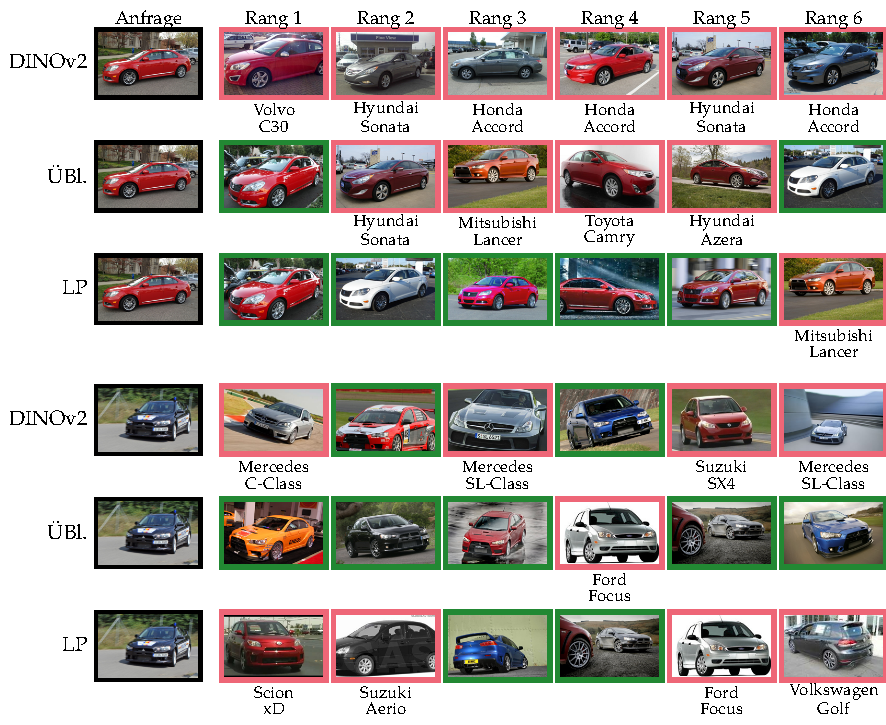
\includegraphics{neu/retrieval_ergebnisse}
  \caption[Retrieval-Beispiele auf Cars196]{Nächste Nachbarn zweier Cars196-Querys für die unveränderten DINOv2-Merkmale, die \UEBL und \acs{LP} (Circle, $k=16$, Seed~2, Concat). Grün umrandet: gleiche Klasse wie die Query, rot: andere Klasse, darunter das Modell. Oben ist \acs{LP} besser als die \UEBL (Suzuki Kizashi), unten schlechter (Mitsubishi Lancer).}
  \label{fig:e:retrieval}
\end{figure}

Abbildung~\ref{fig:e:retrieval} zeigt, wie sich die Unterschiede zwischen der \UEBL und \ac{LP} im Einzelfall äußern. Bei 32 der \num{8131} Querys findet die \UEBL höchstens zwei und \ac{LP} mindestens fünf der sechs nächsten Nachbarn richtig. Nur vier Querys zeigen das umgekehrte Muster. Aus beiden Gruppen ist je eine Limousine derselben Größenklasse gezeigt. Beim Suzuki Kizashi finden die DINOv2-Merkmale Mittelklasselimousinen anderer Hersteller ähnlicher Farbe. Die \UEBL findet neben einem richtigen Treffer ebenfalls vor allem andere Modelle und \ac{LP} findet fast nur Kizashis. Beim Mitsubishi Lancer ist es umgekehrt und \ac{LP} liefert kompakte Autos anderer Hersteller. Im Mittel über alle Querys sind \qty{64.0}{\percent} der sechs nächsten Nachbarn der DINOv2-Merkmale richtig, \qty{83.8}{\percent} bei der \UEBL und \qty{85.0}{\percent} bei \ac{LP}.

\section{Herkunft der ungelabelten Bilder}
\label{sec:e:herkunft}

In den folgenden Abschnitten stammen die ungelabelten Bilder zuerst aus Klassen ohne Labels, danach aus einem externen Datensatz.

\subsection{Bilder aus Klassen ohne Labels}
\label{sec:e:klassen}

In der zweiten In-Shop-Serie ist ein Anteil der Trainingsklassen vollständig gelabelt. Das Muster unterscheidet sich für diese Aufteilung deutlich von der $k$-Serie.

\begin{figure}[tbp]
  \centering
  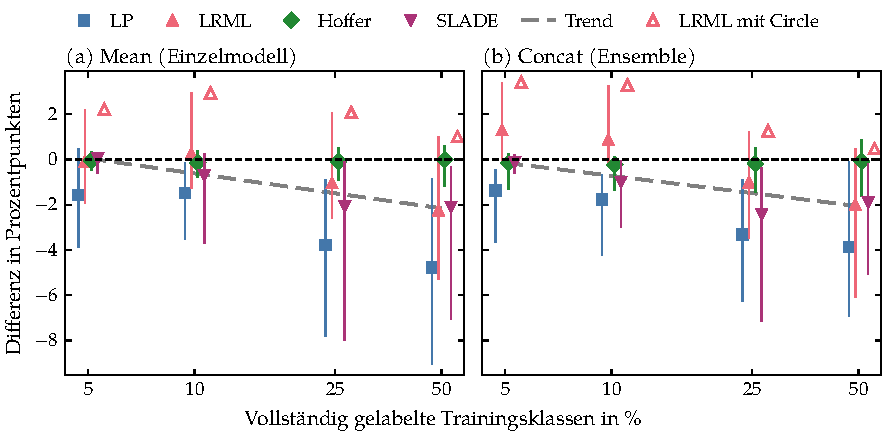
\includegraphics{neu/inshop10_gewinn}
  \caption[In-Shop mit vollständig gelabelten Klassen]{Gepaarter Gewinn der Test-\acs{MAP@R} gegenüber der \UEBL über den Anteil gelabelter Klassen auf In-Shop, (a)~Mean, (b)~Concat, Mittel über die fünf Verlustfunktionen (Striche: Spanne). Hohle Dreiecke: \acs{LRML} mit Circle. Grau gestrichelt: Trend über die vier Verfahren (lineare Anpassung an ihren Median je Anteil).}
  \label{fig:e:klassen}
\end{figure}

Stammen die ungelabelten Bilder aus Klassen ohne Labels, dann hilft nur \ac{LRML} (Abbildung~\ref{fig:e:klassen}). \ac{LP} ist bei jedem Klassenanteil schlechter als die \UEBL, Hoffer liegt nahe null und \ac{SLADE} liegt ab \qty{10}{\percent} gelabelter Klassen unter der \UEBL. \ac{LRML} gewinnt im Ensemble bei 5 und \qty{10}{\percent} gelabelten Klassen mit vier bzw.\ drei der fünf Verlustfunktionen. Als Einzelmodell liegt es dort im Mittel auf dem Niveau der \UEBL. Mit Circle gewinnt \ac{LRML} bei allen Anteilen und in allen Seeds als Einzelmodell wie im Ensemble und erreicht bei 5, 10 und \qty{25}{\percent} die höchste Ensemble-\ac{MAP@R} der Serie. Ab \qty{25}{\percent} gelabelter Klassen ist \ac{LRML} im Mittel über die Verlustfunktionen aber ebenfalls schlechter als die \UEBL. Die Mechanismen, die jedes ungelabelte Bild einer gelabelten Klasse zuordnen, profitieren hier also nicht, \ac{LRML}, das keine solche Zuordnung vornimmt, bei wenigen gelabelten Klassen dagegen schon.%

\begin{table}[tbp]
\centering
\caption[Zerlegung des Gewinns von \acs{LRML} bei Klassen ohne Labels]{Zerlegung des Gewinns von \acs{LRML} in der In-Shop-Serie mit \qty{10}{\percent} vollständig gelabelten Klassen (Seed 2): Änderung der Test-MAP@R gegenüber der regulären Konfiguration in Prozentpunkten, \UEBL und regulär absolut in \%. Varianten wie in Abschnitt \ref{sec:m:phase2}. Rauschschwelle $2\sqrt{2}\,\sigma$ aus den fünf Seeds der Phase 1 bei \qty{10}{\percent} (Abschnitt \ref{sec:m:phase2}).}
\label{tab:e:klassen:2x2}
\footnotesize\setlength{\tabcolsep}{4pt}\renewcommand{\arraystretch}{0.95}
\begin{tabular}{@{}l *{5}{S[table-format=+2.1, retain-explicit-plus]}@{}}
\toprule
{Variante} & {ArcFace} & {Circle} & {\acs{MS}} & {NT-Xent} & {Proxy-Anchor} \\
\midrule
\multicolumn{6}{@{}l}{\textit{Einzelmodell (Mean)}} \\
\quad \UEBL (MAP@R) & 48.2 & 47.7 & 48.4 & 48.1 & 48.0 \\
\quad regulär (MAP@R) & 48.4 & 50.7 & 49.2 & 46.9 & 47.4 \\
\quad Rauschschwelle & 0.9 & 0.2 & 0.5 & 0.4 & 0.5 \\
\quad Hyperparameter der \UEBL & -1.0 & -4.1 & -0.1 & +0.8 & -19.1 \\
\quad ohne ungelabelte Bilder & -0.8 & -2.5 & -1.8 & +0.5 & -0.2 \\
\addlinespace
\multicolumn{6}{@{}l}{\textit{Ensemble (Concat)}} \\
\quad \UEBL (MAP@R) & 52.5 & 52.3 & 52.9 & 51.9 & 51.9 \\
\quad regulär (MAP@R) & 52.9 & 55.4 & 54.7 & 51.8 & 51.6 \\
\quad Rauschschwelle & 1.0 & 0.4 & 1.1 & 0.6 & 0.4 \\
\quad Hyperparameter der \UEBL & +0.3 & -5.0 & -1.7 & +0.0 & -20.2 \\
\quad ohne ungelabelte Bilder & -1.0 & -2.2 & -2.2 & +0.6 & -0.1 \\
\bottomrule
\end{tabular}
\end{table}


Dass \ac{LRML} dabei die Bilder neuer Klassen selbst verwertet, zeigt die $2\times2$-Zerlegung bei \qty{10}{\percent} gelabelter Klassen (Tabelle~\ref{tab:e:klassen:2x2}). Ohne die ungelabelten Bilder verliert \ac{LRML} im Ensemble und als Einzelmodell mit Circle und \ac{MS} deutlich mehr als die Rauschschwelle, also gerade mit den beiden Verlustfunktionen, mit denen es bei diesem Anteil im Ensemble am deutlichsten gewinnt. Mit ArcFace liegt der Verlust an der Rauschschwelle. Mit \ac{NT-Xent} schneidet \ac{LRML} ohne die ungelabelten Bilder dagegen um knapp mehr als die Rauschschwelle besser ab. Mit den Hyperparametern der \UEBL verliert \ac{LRML} vor allem mit Proxy-Anchor (rund 20 Prozentpunkte) und Circle (vier bis fünf Prozentpunkte).%


Bei ähnlichem gelabeltem Anteil des Trainingspools und fast gleicher Leistung der \UEBL (\qty{54.2}{\percent} bei \qty{25}{\percent} gelabelter Klassen, \qty{54.6}{\percent} bei $k=2$) verliert \ac{LP} in dieser Serie \num{3.8} Prozentpunkte und gewinnt in der $k$-Serie \num{3.2}. Am meisten verliert \ac{LP} hier bei jedem Anteil mit ArcFace und Proxy-Anchor (Tabelle~\ref{tab:anhang:inshop10}). Mit ArcFace und Proxy-Anchor bleibt die beste Validierungs-\ac{MAP@R} nach dem Warm-up in 79 bzw.\ 80 von 80 Folds unter der besten des Warm-ups. Mit Circle sind es 66 von 80 Folds, mit \ac{MS} und \ac{NT-Xent} 0 bzw.\ 6. In der $k$-Serie tritt das mit keiner der fünf Verlustfunktionen auf. Mit \ac{MS} und \ac{NT-Xent} liegt die gewählte Konfidenzschwelle so niedrig, dass \ac{LP} von der ersten Aktualisierung an alle ungelabelten Bilder übernimmt, deren Pseudo-Labels ausnahmslos falsch sind, weil keines zu einer gelabelten Klasse gehört.%




\subsection{Externe ungelabelte Bilder}
\label{sec:e:extern}

\begin{table}[tbp]
\centering
\caption[Externe ungelabelte Bilder]{Externe ungelabelte Bilder bei vollständig gelabelten Trainingsklassen (Seed 2): gepaarter Gewinn der Test-MAP@R gegenüber der \UEBL ohne externe Bilder in Prozentpunkten, Mittel über die fünf Verlustfunktionen. Anteil: genutzter Anteil von CompCars (Cars196) bzw.\ Fashion200k (In-Shop), darunter die Bildzahl. Ohne: Kontrolle ohne externe Bilder, bei Hoffer und SLADE mit abgeschaltetem \acs{SSL}-Term. \UEBL: Test-MAP@R in \%. Fett: größter Gewinn je Spalte, sofern er positiv ist. M: Mean, C: Concat.}
\label{tab:e:extern}
\setlength{\tabcolsep}{2.9pt}
\small
\begin{tabular}{@{}ll *{10}{S[table-format=+2.1, retain-explicit-plus]}@{}}
\toprule
 & & \multicolumn{5}{c}{Cars196 + CompCars} & \multicolumn{5}{c}{In-Shop + Fashion200k} \\
\cmidrule(lr){3-7}\cmidrule(lr){8-12}
\multicolumn{2}{@{}l}{Anteil} & {ohne} & {\qty{10}{\percent}} & {\qty{25}{\percent}} & {\qty{50}{\percent}} & {\qty{100}{\percent}} & {ohne} & {\qty{5}{\percent}} & {\qty{10}{\percent}} & {\qty{25}{\percent}} & {\qty{50}{\percent}} \\
\multicolumn{2}{@{}l}{Bilder} & {\num{0}} & {\num{1654}} & {\num{4134}} & {\num{8268}} & {\num{16537}} & {\num{0}} & {\num{16917}} & {\num{33834}} & {\num{84585}} & {\num{169170}} \\
\midrule
\UEBL & M & \multicolumn{5}{c}{\num{43.1}} & \multicolumn{5}{c}{\num{60.1}} \\
 & C & \multicolumn{5}{c}{\num{45.3}} & \multicolumn{5}{c}{\num{60.9}} \\
\addlinespace
\multicolumn{2}{@{}l}{\emph{Gewinn (M)}} & & & & & & & & & & \\
LP & & +0.1 & -5.5 & -5.3 & -5.3 & -4.9 & -1.1 & -8.6 & -8.5 & -8.1 & -8.0 \\
\acs{LRML} & & \bfseries +0.7 & -0.7 & -1.4 & -2.0 & -2.3 & -1.3 & -3.8 & -4.9 & -6.4 & -8.2 \\
Hoffer & & -0.3 & -4.6 & -4.5 & -4.7 & -4.4 & -3.2 & -8.0 & -7.8 & -7.5 & -7.6 \\
SLADE & & +0.4 & -3.7 & -3.6 & -3.7 & -3.7 & -5.0 & -4.0 & -4.1 & -3.9 & -4.0 \\
\addlinespace
\multicolumn{2}{@{}l}{\emph{Gewinn (C)}} & & & & & & & & & & \\
LP & & +0.1 & -6.6 & -6.3 & -6.2 & -6.0 & -1.0 & -8.2 & -8.2 & -7.9 & -7.9 \\
\acs{LRML} & & \bfseries +0.5 & -0.6 & -1.4 & -2.2 & -3.2 & -1.1 & -3.1 & -4.0 & -6.3 & -8.1 \\
Hoffer & & -0.5 & -4.2 & -4.3 & -4.4 & -4.4 & -2.9 & -7.7 & -7.4 & -7.0 & -7.3 \\
SLADE & & +0.4 & -3.9 & -3.9 & -4.1 & -4.1 & -4.7 & -3.8 & -3.9 & -3.7 & -3.7 \\
\bottomrule
\end{tabular}
\end{table}


Mit allen Labels der Trainingsklassen und einem externen ungelabelten Pool wie in der Originalarbeit von \ac{SLADE} liegt kein Mechanismus im Mittel über die Verlustfunktionen über der \UEBL (Tabelle~\ref{tab:e:extern}, Einzelwerte in den Tabellen~\ref{tab:anhang:extern:cars} und~\ref{tab:anhang:extern:inshop}). Auf In-Shop liegen 79 der 80 gepaarten Vergleiche um mehr als die Rauschschwelle unter der \UEBL, auf Cars196 71. \ac{LP}, Hoffer und \ac{SLADE} verlieren fast unabhängig von der Größe des Pools mehrere Prozentpunkte und \ac{LRML} verliert mit wachsendem Pool mehr. Über der \UEBL liegt mit externem Pool nur \ac{LRML} mit \ac{NT-Xent} auf Cars196 bei 10 und \qty{25}{\percent}, allerdings unter der Rauschschwelle.%


Ohne externe Bilder liegen \ac{LP}, Hoffer und \ac{SLADE} auf Cars196 auf dem Niveau der \UEBL, \ac{LRML} liegt leicht darüber (Spalte \enquote{ohne} in Tabelle~\ref{tab:e:extern}). Die Verluste auf Cars196 entstehen also erst mit den externen Bildern, bei \ac{LP}, Hoffer und \ac{SLADE} zugleich mit ihrem Mechanismus, der in der Kontrolle fehlt. Auf In-Shop liegen dagegen schon diese Kontrollen im Mittel unter der \UEBL, mit \ac{LP} und \ac{LRML} um gut einen Prozentpunkt, mit Hoffer und \ac{SLADE} um mehrere Prozentpunkte. Bei \ac{LP} geht dieses Mittel allein auf ArcFace zurück (\num{-9.7} Prozentpunkte). Mit den übrigen vier Verlustfunktionen liegt die Kontrolle um mehr als die Rauschschwelle über der \UEBL. Bei \ac{SLADE} bestimmen es Proxy-Anchor (\num{-18.3}) und ArcFace (\num{-8.1}). Andere Nachbar- und Clusterzahlen ändern das Bild auf Cars196 kaum (Tabelle~\ref{tab:anhang:extern:sweeps}). In den verwendeten Konfigurationen von \ac{LP} stammen auf Cars196 \num{12.5} bis \qty{25}{\percent} jedes Batches aus den gelabelten Bildern, auf In-Shop \qty{50}{\percent}.%



\section{Worauf der Nutzen beruht}
\label{sec:e:phase2}
Die Ablationen der Phase~2 laufen auf Cars196 bei $k=16$ und $k=8$ und auf In-Shop bei $k=2$, jeweils mit allen vier Mechanismen und allen fünf Verlustfunktionen. Wo nicht anders angegeben, beziehen sich die folgenden Abschnitte auf Cars196 mit $k=16$ und auf In-Shop.  Tabelle~\ref{tab:e:ablationen:verluste} gibt für jede Kombination die Änderung gegenüber der regulären Konfiguration an, Anhang~\ref{chap:anhang:phase2} enthält alle Einzelwerte. Als Befund gilt ein Unterschied erst oberhalb der Rauschschwelle aus Abschnitt~\ref{sec:m:phase2}, die für jede Kombination aus Mechanismus und Verlustfunktion getrennt bestimmt wird.

\begin{table}[tbp]
\centering
\caption[Ablationen der Phase 2 auf Cars196 und In-Shop]{Ablationen der Phase 2 auf Cars196 und In-Shop (Seed 2): Änderung der Test-MAP@R (Mean) gegenüber der regulären Konfiguration in Prozentpunkten, \UEBL und regulär absolut in \%. Eingriffe wie in Tabelle \ref{tab:phase2:eingriffe} und Abschnitt \ref{sec:m:phase2}, eingefroren: Pseudo-Labels bzw.\ Graph. Fett: Änderung größer als die Rauschschwelle. Ohne Warm-up: gleich der regulären Konfiguration, wo Phase 1 kein Warm-up gewählt hat. Arc: ArcFace, Cir: Circle, NT: NT-Xent, PA: Proxy-Anchor.}
\label{tab:e:ablationen:verluste}
\footnotesize\setlength{\tabcolsep}{3.2pt}\setlength{\hfuzz}{1.2pt}\renewcommand{\arraystretch}{0.95}
\begin{tabular}{@{}l *{5}{S[table-format=+2.1, retain-explicit-plus]} @{\hspace{12pt}} *{5}{S[table-format=+2.1, retain-explicit-plus]}@{}}
\toprule
& \multicolumn{5}{c}{\textbf{Cars196} ($k=16$)} & \multicolumn{5}{c}{\textbf{In-Shop} ($k=2$)} \\
\cmidrule(lr){2-6}\cmidrule(l){7-11}
{Variante} & {Arc} & {Cir} & {\acs{MS}} & {NT} & {PA} & {Arc} & {Cir} & {\acs{MS}} & {NT} & {PA} \\
\midrule
\textit{\UEBL (MAP@R)} & 40.3 & 39.1 & 40.8 & 39.2 & 39.2 & 54.8 & 54.7 & 56.1 & 54.6 & 53.8 \\
\midrule
\multicolumn{11}{@{}l}{\textbf{LP}} \\
\quad\textit{regulär (MAP@R)} & 41.9 & 42.3 & 43.3 & 41.4 & 42.6 & 58.9 & 57.8 & 58.8 & 58.0 & 56.3 \\
\quad\textit{Rauschschwelle} & 0.8 & 0.5 & 0.6 & 0.6 & 0.3 & 0.1 & 0.3 & 0.2 & 0.4 & 0.4 \\
\cmidrule{1-11}
\quad SSL-Mechanismus abgeschaltet & \bfseries -4.5 & \bfseries -3.2 & \bfseries -2.7 & \bfseries -2.2 & \bfseries -2.7 & \bfseries -10.8 & \bfseries -3.1 & \bfseries -3.0 & \bfseries -4.2 & \bfseries -3.4 \\
\quad Hyperparameter der \UEBL & -0.5 & -0.5 & +0.5 & +0.1 & \bfseries -2.4 & \bfseries -0.7 & \bfseries -1.0 & +0.2 & \bfseries -0.7 & \bfseries -2.6 \\
\quad ohne Warm-up & \bfseries -1.0 & +0.1 & -0.4 & +0.0 & +0.0 & -0.1 & -0.1 & \bfseries +0.2 & -0.1 & \bfseries -0.4 \\
\addlinespace[2pt]
\quad eingefroren & -0.3 & \bfseries -0.9 & \bfseries -0.7 & -0.2 & \bfseries -1.4 & \bfseries -11.5 & \bfseries -2.5 & \bfseries -0.7 & \bfseries -2.2 & \bfseries -1.3 \\
\quad Graph umverdrahtet & \bfseries -14.2 & \bfseries -8.6 & \bfseries -12.3 & \bfseries -6.3 & \bfseries -10.0 & \bfseries -13.4 & \bfseries -10.2 & \bfseries -9.5 & \bfseries -11.5 & \bfseries -8.9 \\
\quad Oracle-Kanten entfernt & -0.2 & \bfseries +0.9 & +0.6 & \bfseries +1.2 & \bfseries +1.0 & \bfseries -8.2 & \bfseries +2.2 & \bfseries +1.4 & \bfseries +1.7 & \bfseries +2.0 \\
\quad zufällige Kanten entfernt & -0.1 & +0.2 & -0.4 & +0.2 & +0.1 & \bfseries -22.6 & \bfseries -4.1 & +0.2 & +0.1 & -0.1 \\
\midrule
\multicolumn{11}{@{}l}{\textbf{\acs{LRML}}} \\
\quad\textit{regulär (MAP@R)} & 40.9 & 40.9 & 40.4 & 39.9 & 41.7 & 58.0 & 57.6 & 56.6 & 55.7 & 53.7 \\
\quad\textit{Rauschschwelle} & 0.5 & 0.7 & 1.1 & 0.7 & 0.5 & 1.3 & 0.3 & 0.7 & 0.4 & 0.7 \\
\cmidrule{1-11}
\quad SSL-Mechanismus abgeschaltet & \bfseries -5.3 & \bfseries -2.1 & \bfseries -4.4 & \bfseries -3.1 & \bfseries -3.1 & \bfseries -11.0 & \bfseries -4.6 & \bfseries -2.5 & \bfseries -2.6 & \bfseries -2.7 \\
\quad ohne ungelabelte Bilder & \bfseries -3.1 & -0.4 & \bfseries -1.9 & -0.7 & \bfseries -1.1 & \bfseries -3.3 & \bfseries -4.1 & \bfseries -2.8 & \bfseries -2.5 & \bfseries -2.3 \\
\quad Hyperparameter der \UEBL & \bfseries -4.1 & +0.0 & +0.1 & \bfseries -3.2 & \bfseries -3.8 & \bfseries -5.6 & \bfseries -1.6 & +0.6 & \bfseries -1.0 & +0.4 \\
\quad ohne Warm-up & \bfseries -9.6 & -0.7 & \bfseries -2.2 & \bfseries -6.4 & \bfseries -2.1 & \bfseries -8.4 & -0.3 & -0.3 & -0.1 & \bfseries +0.7 \\
\addlinespace[2pt]
\quad eingefroren & -0.5 & -0.2 & -0.6 & +0.1 & -0.1 & \bfseries -1.3 & \bfseries -1.8 & -0.2 & -0.3 & \bfseries -2.3 \\
\quad Graph umverdrahtet & \bfseries -5.1 & \bfseries -2.2 & \bfseries -5.6 & \bfseries -2.8 & \bfseries -3.2 & \bfseries -11.4 & \bfseries -11.6 & \bfseries -4.4 & \bfseries -4.9 & \bfseries -2.6 \\
\quad Oracle-Kanten entfernt & +0.4 & +0.5 & +0.8 & +0.6 & \bfseries +0.7 & +1.2 & \bfseries +1.4 & \bfseries +0.9 & \bfseries +1.2 & \bfseries +0.7 \\
\quad zufällige Kanten entfernt & +0.2 & +0.1 & -0.3 & +0.3 & +0.0 & -0.1 & -0.1 & +0.1 & +0.1 & +0.1 \\
\midrule
\multicolumn{11}{@{}l}{\textbf{Hoffer}} \\
\quad\textit{regulär (MAP@R)} & 40.5 & 40.6 & 39.5 & 40.3 & 40.6 & 57.7 & 58.1 & 57.9 & 58.2 & 57.6 \\
\quad\textit{Rauschschwelle} & 0.3 & 0.4 & 0.5 & 0.7 & 0.5 & 0.2 & 0.2 & 0.2 & 0.2 & 0.3 \\
\cmidrule{1-11}
\quad SSL-Mechanismus abgeschaltet & \bfseries -1.3 & \bfseries -1.7 & \bfseries -0.9 & \bfseries -2.2 & \bfseries -1.1 & \bfseries -5.0 & \bfseries -3.7 & \bfseries -4.8 & \bfseries -6.2 & \bfseries -5.7 \\
\quad ohne ungelabelte Bilder & \bfseries -2.3 & \bfseries -1.3 & \bfseries -1.0 & \bfseries -1.8 & \bfseries -1.3 & \bfseries -4.1 & \bfseries -3.6 & \bfseries -4.0 & \bfseries -3.5 & \bfseries -4.0 \\
\quad Hyperparameter der \UEBL & +0.1 & \bfseries -1.3 & -0.2 & -0.7 & \bfseries -1.6 & \bfseries -0.6 & \bfseries -0.6 & \bfseries -0.9 & \bfseries -1.1 & \bfseries -1.0 \\
\quad ohne Warm-up & \bfseries -0.3 & \bfseries -1.0 & \bfseries -0.6 & -0.2 & +0.0 & \bfseries -0.5 & -0.1 & \bfseries -0.2 & -0.2 & +0.0 \\
\midrule
\multicolumn{11}{@{}l}{\textbf{SLADE}} \\
\quad\textit{regulär (MAP@R)} & 40.2 & 41.6 & 41.7 & 40.6 & 40.4 & 53.7 & 54.8 & 54.5 & 54.1 & 53.7 \\
\quad\textit{Rauschschwelle} & 1.0 & 0.6 & 1.0 & 0.3 & 0.6 & 1.4 & 0.4 & 0.4 & 0.5 & 0.9 \\
\cmidrule{1-11}
\quad SSL-Mechanismus abgeschaltet & -0.7 & \bfseries -3.1 & \bfseries -1.5 & \bfseries -2.3 & \bfseries -1.5 & -1.0 & -0.1 & \bfseries -1.8 & +0.0 & \bfseries -10.6 \\
\quad ohne ungelabelte Bilder & -0.2 & \bfseries -3.5 & -0.8 & \bfseries -1.8 & \bfseries -0.9 & +0.3 & -0.3 & \bfseries -0.5 & +0.1 & +0.0 \\
\quad Hyperparameter der \UEBL & \bfseries -4.5 & -0.5 & \bfseries -2.8 & \bfseries -5.3 & \bfseries -2.1 & \bfseries -7.1 & \bfseries -1.4 & \bfseries -3.4 & -0.3 & \bfseries -1.6 \\
\quad ohne Warm-up & \bfseries -1.2 & \bfseries -2.1 & -0.4 & \bfseries -1.4 & +0.0 & +0.0 & -0.2 & -0.1 & +0.1 & -0.1 \\
\bottomrule
\end{tabular}
\end{table}


\subsection{Hyperparameter, Term oder ungelabelte Bilder?}
\label{sec:e:2x2}

Die \ac{SSL}-Konfigurationen wurden separat optimiert. Abbildung~\ref{fig:e:2x2:verluste} zeigt die Varianten der $2\times2$-Zerlegung und die Kontrolle mit abgeschaltetem \ac{SSL}-Term als Differenz zur \UEBL.

Die reguläre Konfiguration übertrifft die \UEBL in 26 der 40 Kombinationen um mehr als die Rauschschwelle (Abbildung~\ref{fig:e:2x2:verluste}). Auf Cars196 gewinnt \ac{LP} mit allen fünf Verlustfunktionen, Hoffer und \ac{SLADE} mit je drei und \ac{LRML} mit zwei. Auf In-Shop gewinnen \ac{LP} und Hoffer mit allen fünf, \ac{LRML} mit drei und \ac{SLADE} mit keiner. Im Mittel der fünf Seeds der Phase~1 liegen sechs der 14 Kombinationen ohne Gewinn über der \UEBL (Anhang~\ref{chap:anhang:ergebnisse}).%


\begin{figure}[tbp]
  \centering
  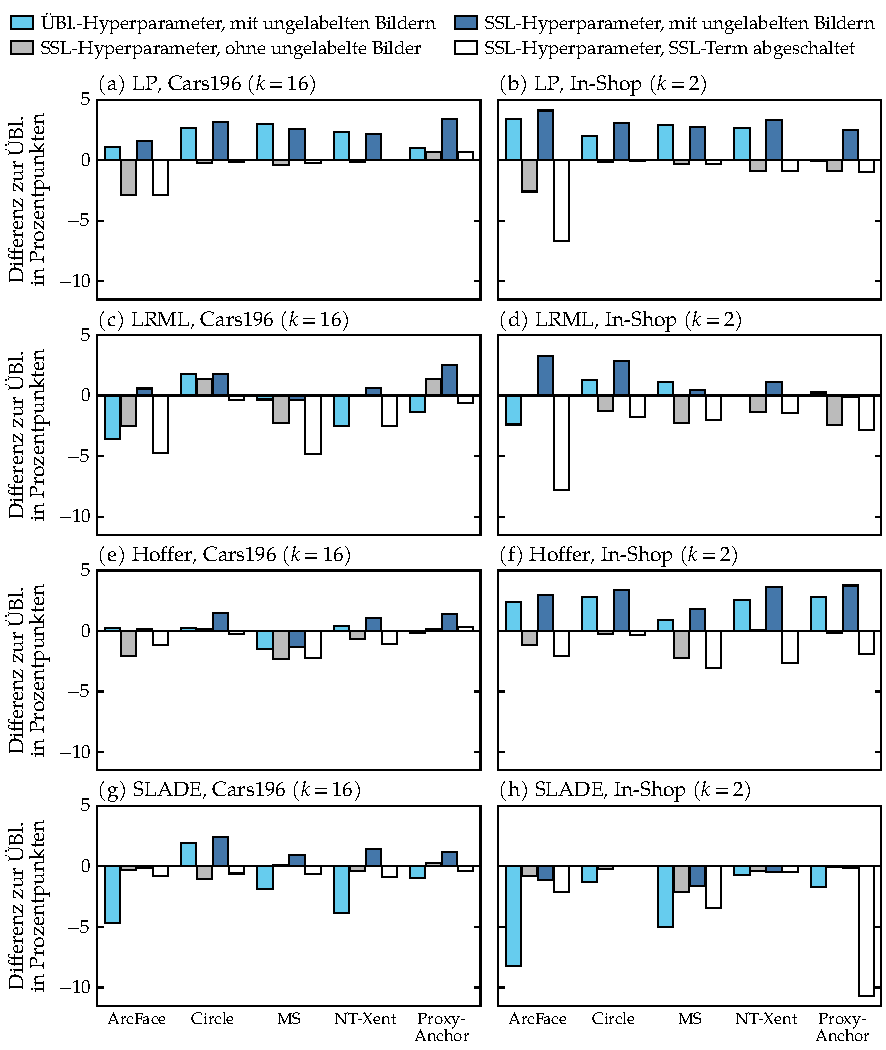
\includegraphics{neu/phase2_2x2_verluste}
  \caption[Zerlegung des Gewinns nach Hyperparametern, \acs{SSL}-Term und ungelabelten Bildern]{Zerlegung des Gewinns mit allen fünf Verlustfunktionen auf Cars196 ($k=16$, links) und In-Shop ($k=2$, rechts), zeilenweise für \acs{LP}, \acs{LRML}, Hoffer und \acs{SLADE}: Test-\acs{MAP@R} der Einzelmodelle als Differenz zur \UEBL, ein Seed. Varianten wie in Tabelle~\ref{tab:m:2x2}, dazu die Kontrolle mit abgeschaltetem \acs{SSL}-Term (Tabelle~\ref{tab:phase2:eingriffe}).}
  \label{fig:e:2x2:verluste}
\end{figure}

Die abweichenden Hyperparameter allein erklären den Gewinn nicht. Die ungelabelten Bilder leisten in den meisten Kombinationen einen eigenen Beitrag. Mit den \ac{SSL}-Hyperparametern senkt das Entfernen der ungelabelten Bilder die Leistung in 37 der 40 Kombinationen, in 32 um mehr als die Rauschschwelle. Die Kontrolle mit denselben Hyperparametern und abgeschaltetem \ac{SSL}-Term liegt dagegen nur in einer Kombination um mehr als die Rauschschwelle über der \UEBL und in 25 darunter. Ohne den Term sind die \ac{SSL}-Hyperparameter also oft sogar schlechter als die der \UEBL.%


Was der \ac{SSL}-Term ohne ungelabelte Bilder bewirkt, zeigt der Vergleich der Variante ohne ungelabelte Bilder mit der Kontrolle mit abgeschaltetem \ac{SSL}-Term (Abschnitt~\ref{sec:m:phase2}). In 18 der 40 Kombinationen liegt die Variante ohne ungelabelte Bilder um mehr als die Rauschschwelle über dieser Kontrolle. Das gilt bei \ac{LRML} auf Cars196 für alle fünf Verlustfunktionen und bei Hoffer auf In-Shop für vier, bei \ac{LP} nur in einer Kombination.

Für \ac{LRML} auf Cars196 enthält der Pool dieser Variante bei $k=16$ höchstens 15 weitere Bilder derselben Klasse je Bild. Bei den gewählten 39 bis 81 Nachbarn muss deshalb schon durch die Konstruktion die Mehrheit der Nachbarschaftsbeziehungen zu anderen Klassen führen. In sieben der 18 Kombinationen bleibt die Variante ohne ungelabelte Bilder um mehr als die Rauschschwelle unter der \UEBL.%


Die Variante mit den Hyperparametern der \UEBL misst den Term und die ungelabelten Bilder gemeinsam (Abschnitt~\ref{sec:m:phase2}). Auf Cars196 liegt sie um mehr als die Rauschschwelle über der \UEBL bei \ac{LP} mit allen fünf Verlustfunktionen, bei \ac{LRML} und \ac{SLADE} nur mit Circle und bei Hoffer mit keiner. In sechs der 15 Kombinationen von \ac{LRML}, Hoffer und \ac{SLADE} gewinnt die reguläre Konfiguration auf Cars196 also nur mit den eigens abgestimmten Hyperparametern. Auf In-Shop liegt sie dagegen bei \ac{LP} mit vier, bei Hoffer mit allen fünf, bei \ac{LRML} mit zwei und bei \ac{SLADE} mit keiner Verlustfunktion um mehr als die Rauschschwelle über der \UEBL. Da dort ohne ungelabelte Bilder keine Kombination über der \UEBL liegt, stammt der Gewinn von \ac{LP}, \ac{LRML} und Hoffer auf In-Shop von den ungelabelten Bildern. Bei \ac{SLADE} ändert das Entfernen der ungelabelten Bilder die Leistung auf In-Shop nur in einer Kombination um mehr als die Rauschschwelle.%

Bei $k=8$ (Tabelle~\ref{tab:anhang:phase2:k8} in Anhang~\ref{chap:anhang:phase2}) übertrifft die reguläre Konfiguration der \ac{SSL}-Methoden die \UEBL in 18 der 20 Kombinationen um mehr als die Rauschschwelle, das Entfernen der ungelabelten Bilder kostet in allen 20 Leistung und die Kontrolle mit abgeschaltetem \ac{SSL}-Term liegt nur bei \ac{LP} mit Proxy-Anchor über der \UEBL. Auch bei $k=8$ tragen also die ungelabelten Bilder und die \ac{SSL}-Methoden den Gewinn und nicht die separat gewählten Hyperparameter allein.%


\subsection{Qualität der Pseudo-Labels}
\label{sec:e:pseudolabels}

Die gewählte Konfidenzschwelle liegt meist so niedrig, dass \ac{LP} schon bei der ersten Aktualisierung fast jedes ungelabelte Bild übernimmt (Mittel über die vier Folds, solange alle trainieren). Auf Cars196 sind diese Pseudo-Labels anfangs zu \qty{77}{\percent} bis \qty{84}{\percent} richtig, auf In-Shop zu \qty{60}{\percent} bis \qty{69}{\percent}. Bis zum Ende des Trainings steigt ihre Genauigkeit, auf Cars196 auf \qty{85}{\percent} bis \qty{87}{\percent}. Eine Ausnahme ist Circle auf Cars196, wo die Konfidenzschwelle anfangs gut ein Drittel der Bilder ausschließt. Eine weitere Ausnahme ist ArcFace auf In-Shop, wo \ac{LP} anfangs nur \qty{5}{\percent} der Bilder übernimmt. Obwohl auf In-Shop am Ende noch rund ein Viertel der Pseudo-Labels falsch ist, liegt \ac{LP} dort mit jeder Verlustfunktion über der \UEBL.%


Auf Semi-iNat-2021 übernimmt \ac{LP} bei $k=2$ bei der ersten Aktualisierung \qty{82}{\percent} bis \qty{100}{\percent} der ungelabelten Bilder. Die Pseudo-Labels dieser Bilder sind zu \qty{57}{\percent} bis \qty{71}{\percent} richtig, ein ähnlicher Anteil wie anfangs auf In-Shop. \ac{LP} gewinnt auf Semi-iNat-2021 als Einzelmodell jedoch nur \num{0.6} Prozentpunkte, auf In-Shop dagegen \num{3.2} (Abschnitt~\ref{sec:e:phase1}). Bis zum Ende des Trainings ändert sich der Anteil richtiger Pseudo-Labels um höchstens \num{6.0} Prozentpunkte und liegt dann bei \qty{63}{\percent} bis \qty{71}{\percent}. Bei $k=100$ sind anfangs \qty{79}{\percent} bis \qty{97}{\percent} und am Ende \qty{80}{\percent} bis \qty{96}{\percent} der übernommenen Pseudo-Labels richtig. Dennoch liegt \ac{LP} dort in allen 25 Vergleichen unter der \UEBL.%


\begin{figure}[tbp]
  \centering
  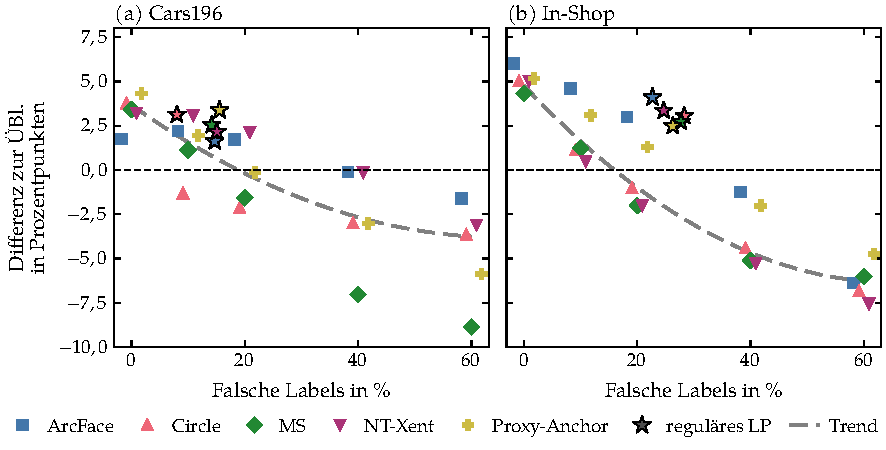
\includegraphics{neu/phase2_lp_qualitaet}
  \caption[Wirkung falscher Pseudo-Labels von \acs{LP}]{Oracle-Pseudo-Labels von \acs{LP}, von denen ein Anteil zufällig falsch ist, mit allen fünf Verlustfunktionen auf (a)~Cars196 ($k=16$) und (b)~In-Shop ($k=2$), ein Seed, als Differenz zur \UEBL. Sterne: reguläres \acs{LP} an seiner über Epochen und Folds gemittelten Fehlerrate. Grau gestrichelt: Trend über die Verlustfunktionen (quadratische Anpassung an ihren Median je Anteil).}
  \label{fig:e:lpqualitaet}
\end{figure}

Wo die falschen Pseudo-Labels liegen und was sich an ihnen während des Trainings ändert, zeigt Abbildung~\ref{fig:e:lpcars} für Cars196 an einem Fold mit Circle bei $k=16$. Abbildung~\ref{fig:e:lpcars}a zeigt die Embeddings und die Pseudo-Labels nach der ersten Epoche mit \ac{LP}. Auf Cars196 bilden nach dem Warm-up viele Klassen schon kompakte Gruppen, deren ungelabelte Bilder fast alle ein richtiges Pseudo-Label erhalten. Bis zum Ende des Trainings steigt die Abdeckung von \qty{63}{\percent} auf \qty{86}{\percent}, während die Genauigkeit der übernommenen Pseudo-Labels von \qty{94}{\percent} auf \qty{92}{\percent} sinkt. Die schon übernommenen Pseudo-Labels ändern sich dagegen kaum. Fast alle richtigen bleiben richtig und die meisten falschen behalten ihre falsche Klasse.%


\begin{figure}[tbp]
  \centering
  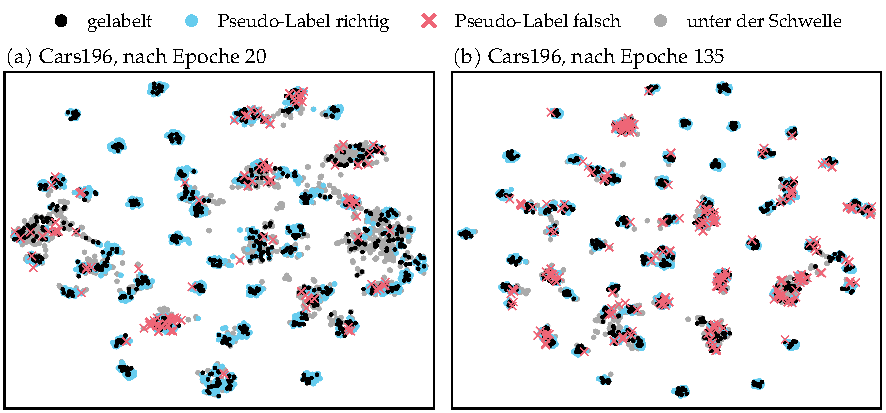
\includegraphics{neu/lp_cars}
  \caption[Label Propagation in einem Graphlauf auf Cars196]{Pseudo-Labels von \acs{LP} in einem Graphlauf auf Cars196 (Circle, $k=16$, Seed~2, Fold~0), \acs{t-SNE} der 4000 verfolgten Bilder des Trainingspools. Gezeigt sind die Pseudo-Labels, die das Training für die jeweils folgende Epoche übernimmt, berechnet aus dem Modell (a)~nach Epoche~20, der ersten nach dem Warm-up aus den Epochen 0 bis 19, (b)~nach Epoche~135 (Training bis Epoche~140). Ob ein Pseudo-Label richtig ist, zeigen die verdeckten Labels. Konfidenzschwelle \num{0.81}. Jede Teilabbildung beruht auf einer eigenen \acs{t-SNE}-Darstellung, die Lage einzelner Gruppen ist zwischen den Teilabbildungen daher nicht vergleichbar.}
  \label{fig:e:lpcars}
\end{figure}

Mit allen fünf Verlustfunktionen nennen die meisten falschen Pseudo-Labels auf Cars196 ein Modell desselben Herstellers. Über alle vier Folds ($k=16$) sind es je nach Verlustfunktion und Fold \qty{67}{\percent} bis \qty{88}{\percent} bei der ersten Aktualisierung, während bei zufälliger Verwechslung höchstens \qty{18}{\percent} zu erwarten wären.

Im entsprechenden Graphlauf auf Semi-iNat-2021 hat die Suche kein Warm-up gewählt, sodass \ac{LP} die ersten Pseudo-Labels aus dem Head vor dem Training berechnet und fast jedes ungelabelte Bild übernimmt. Anders als auf Cars196 wechselt bis zum Ende des Trainings etwa jedes siebte Pseudo-Label die Art. Nur zwei von fünf Wechseln berichtigen dabei ein falsches Pseudo-Label, sodass die Genauigkeit nur von \qty{74}{\percent} auf \qty{78}{\percent} steigt. Das Training ändert auf Cars196 also mit Circle vor allem, welche Bilder ein Pseudo-Label erhalten, mit den übrigen Verlustfunktionen dagegen, wie viele davon richtig sind. Auf Semi-iNat-2021 ändert es vor allem, welche Art die Pseudo-Labels nennen.%

Abbildung~\ref{fig:e:lpqualitaet} stellt den Fehlern von \ac{LP} auf Cars196 und In-Shop kontrollierte Fehler gegenüber. Erhalten genau die von \ac{LP} übernommenen Bilder ihr wahres Label, steigt die Leistung gegenüber der regulären Konfiguration auf Cars196 mit vier Verlustfunktionen um bis zu \num{1.1} Prozentpunkte und auf In-Shop mit allen fünf um bis zu \num{2.7}. Zufällig falsche Labels schaden auf In-Shop mit jeder Verlustfunktion deutlich. Auf Cars196 hängt der Schaden von der Verlustfunktion ab, mit Circle, \ac{MS} und Proxy-Anchor machen \qty{20}{\percent} zufällig falscher Labels den Gewinn zunichte, mit ArcFace und \ac{NT-Xent} liegt \ac{LP} auch dann noch über der \UEBL.%


Die vorab festgelegte Erwartung, dass reguläres \ac{LP} auf der Kurve der zufälligen Fehler liegt, trifft auf Cars196 nur mit ArcFace und \ac{NT-Xent} zu, wo schon zufällige Fehler kaum schaden. Mit den übrigen drei Verlustfunktionen auf Cars196 und mit allen fünf auf In-Shop liegt reguläres \ac{LP} über der Kurve, auf In-Shop um bis zu \num{6.1} Prozentpunkte. Mit der Fehlerrate der per Validierung gewählten Epoche statt der über alle Epochen gemittelten ändert sich der Abstand zur Kurve um weniger als einen halben Prozentpunkt. Reguläres \ac{LP} liegt dort also über den Läufen mit zufälligen Fehlern gleicher mittlerer Häufigkeit. Worauf dieser Abstand beruht, trennt der Vergleich nicht, denn die Varianten unterscheiden sich auch in den betroffenen Bildern und im Verlauf des Trainings.%


\subsection{Nachbarschaftsstruktur}
\label{sec:e:nachbarschaft}

Ob die konkrete Nachbarschaft der Daten den Gewinn trägt, prüfen Eingriffe in den Graphen von \ac{LP} und \ac{LRML}. Ein unter Erhalt der Knotengrade zufällig umverdrahteter Graph lässt die Leistung in allen 20 Kombinationen einbrechen, bei \ac{LP} um mindestens \num{6.3} Prozentpunkte. Beide Mechanismen liegen damit in jeder Kombination unter der \UEBL, nur \ac{LRML} mit Circle auf Cars196 innerhalb der Rauschschwelle. Ein beliebiger Zusatzterm hilft also nicht und ein Graph ohne Bezug zu den Daten schadet.%


Ein reinerer Graph hilft. Werden alle Kanten zwischen verschiedenen Klassen entfernt, steigt die Leistung in 18 der 20 Kombinationen, vor allem bei \ac{LP} und bei \ac{LRML} auf In-Shop über der Rauschschwelle. Die Ausnahme ist \ac{LP} mit ArcFace, das auf In-Shop um \num{8.2} Prozentpunkte verliert. Wird stattdessen dieselbe Zahl zufälliger Kanten entfernt, ändert sich die Leistung in 18 der 20 Kombinationen kaum. Nur \ac{LP} auf In-Shop verliert dabei mit Circle und ArcFace deutlich. Bei Circle erklärt die Zahl der entfernten Kanten das allein nicht, denn das Entfernen verschiedenklassiger Kanten hilft dort. Mit ArcFace bricht \ac{LP} auf In-Shop bei den meisten Eingriffen ein (Abschnitt~\ref{sec:e:sweeps}).%


 Auf Cars196 werden die Graphen von \ac{LP} und \ac{LRML} durch das Training um \num{29.5} bis \num{44.4} Prozentpunkte reiner. Danach verlaufen aber noch \qty{15}{\percent} bis \qty{40}{\percent} ihrer Kanten zwischen verschiedenen Klassen, genau die Kanten, die der Eingriff mit den verdeckten Labels entfernt. Auf In-Shop begrenzt die Klassengröße die Reinheit großer Graphen. In den Graphen von \ac{LP} mit ArcFace und Circle, die 83 bzw.\ 95 Nachbarn verwenden, verlaufen nach dem Training weniger als \qty{10}{\percent} der Kanten innerhalb einer Klasse. Beide Eingriffe entfernen deshalb über \qty{90}{\percent} der Kanten. Der Eingriff mit den verdeckten Labels behält dabei alle Kanten innerhalb einer Klasse, die zufällige Kontrolle entfernt auch von diesen über \qty{90}{\percent}. Das passt dazu, dass \ac{LP} mit Circle nur in der zufälligen Kontrolle einbricht. Kleine Graphen mit zwei bis sechs Nachbarn sind auf In-Shop nach dem Training zu mehr als der Hälfte rein. Auf Semi-iNat-2021 sind die Graphen schon vor dem Training zu mehr als der Hälfte rein und werden durch das Training nur um wenige Prozentpunkte reiner, ebenso der Graph mit zehn Nachbarn unter der \UEBL.%





Auch die Aktualisierung zählt. Werden die Pseudo-Labels nach dem Warm-up eingefroren, verliert \ac{LP} auf In-Shop mit jeder Verlustfunktion mehr als die Rauschschwelle (mit ArcFace \num{11.5} Prozentpunkte) und auf Cars196 mit drei Verlustfunktionen. Ein eingefrorener Graph kostet \ac{LRML} auf In-Shop mit drei Verlustfunktionen deutlich, wobei es auf Cars196 kaum etwas kostet.%


\subsection{Einzelne Hyperparameter}
\label{sec:e:sweeps}

Die Abbildungen~\ref{fig:e:sweeps} und~\ref{fig:e:sweeps:inshop} zeigen die Sweeps einzelner Hyperparameter mit allen fünf Verlustfunktionen. Vier Befunde haben mit allen Verlustfunktionen dieselbe Richtung. Erstens ist die beste Nachbarzahl für \ac{LRML} auf In-Shop viel kleiner als auf Cars196. Auf In-Shop sind zwei bis drei Nachbarn mit jeder Verlustfunktion am besten und mehr Nachbarn kosten deutlich. Auf Cars196 sind dagegen 25 bis 100 Nachbarn etwa gleich gut, während sehr wenige und sehr viele Nachbarn schaden. Die Phase~1 hatte auf Cars196 39 bis 81 und auf In-Shop zwei oder drei Nachbarn gewählt. Ob die beste Nachbarzahl allgemein der Klassengröße folgt, lässt sich mit zwei Datensätzen nicht entscheiden.%


\begin{figure}[tbp]
  \centering
  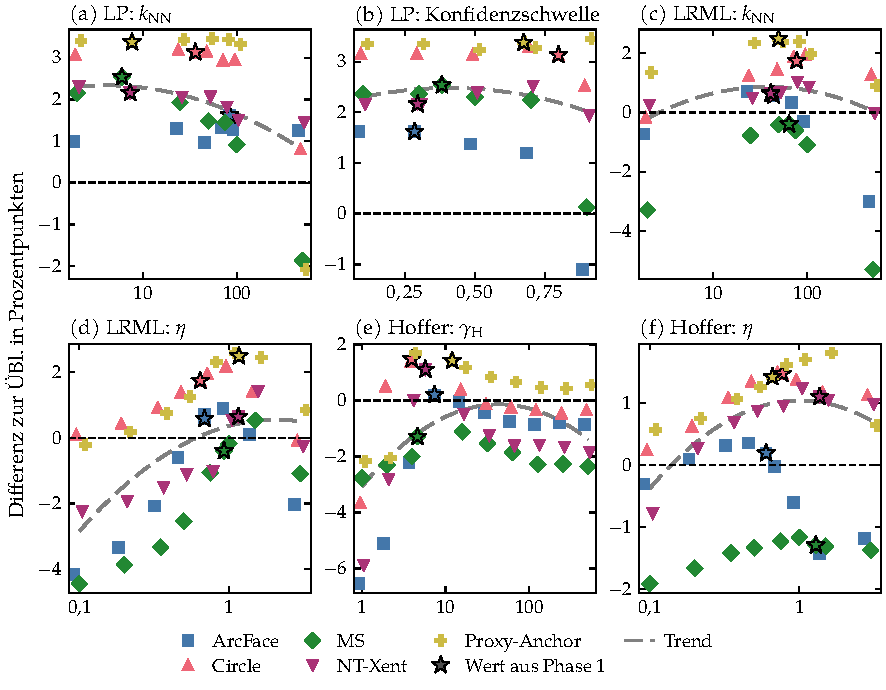
\includegraphics{neu/phase2_sweeps_verluste}
  \caption[Sweeps einzelner Hyperparameter auf Cars196]{Gewinn der Test-\acs{MAP@R} der Einzelmodelle gegenüber der \UEBL bei Variation eines Hyperparameters auf Cars196 ($k=16$, ein Seed, übrige Werte wie in Phase~1). Stern: in Phase~1 gewählter Wert. Grau gestrichelt: Trend über die Verlustfunktionen (quadratische Anpassung an ihren Median je Wert). Logarithmische $x$-Achsen außer bei der Konfidenzschwelle.}
  \label{fig:e:sweeps}
\end{figure}

\begin{figure}[tbp]
  \centering
  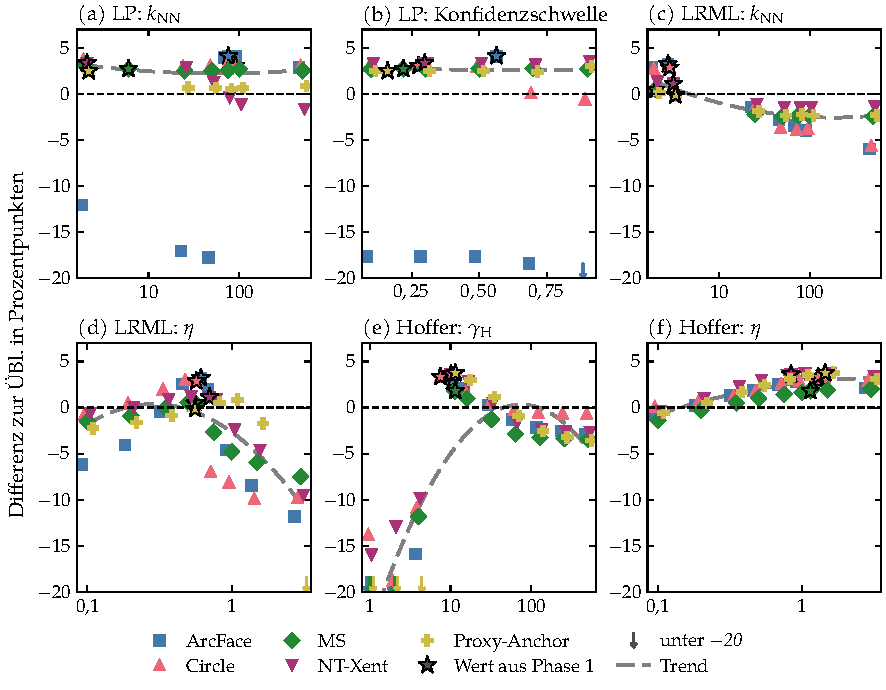
\includegraphics{neu/phase2_sweeps_verluste_inshop}
  \caption[Sweeps einzelner Hyperparameter auf In-Shop]{Sweeps wie in Abbildung~\ref{fig:e:sweeps} auf In-Shop ($k=2$). Die $y$-Achse ist bei \num{-20} Prozentpunkten abgeschnitten, Pfeile markieren Werte darunter. Einzelwerte in Tabelle~\ref{tab:anhang:phase2:inshop}.}
  \label{fig:e:sweeps:inshop}
\end{figure}

Zweitens schadet bei \ac{LRML} ein zu kleines wie ein zu großes $\eta$. Ein kleines $\eta=\num{0.1}$ kostet auf beiden Datensätzen mit jeder Verlustfunktion Leistung, ein großes $\eta=3$ vor allem auf In-Shop, dort um mindestens \num{8.0} Prozentpunkte. Ab welchem Wert die Leistung auf In-Shop einbricht, hängt von der Verlustfunktion ab, mit Circle schon ab $\eta=\num{0.75}$, mit Proxy-Anchor erst bei $\eta=3$.%


Drittens scheitert Hoffer vor allem an einer zu kleinen Distanzskala, wobei eine zu große weniger schadet. Auf In-Shop kosten Distanzskalen $\gamma_{\mathrm{H}}\le4$ mit jeder Verlustfunktion mehr als 13 Prozentpunkte, auf Cars196 Distanzskalen $\gamma_{\mathrm{H}}\le2$ bis zu sieben. Deutliche Verluste treten damit auch oberhalb der notwendigen Mindestskalen aus Abschnitt~\ref{sec:m:hoffer} auf.%


Viertens schadet bei Hoffer auch ein zu kleines $\eta$. Mit $\eta=\num{0.1}$ verliert Hoffer mit jeder Verlustfunktion mehr als die Rauschschwelle, auf In-Shop mindestens \num{3.2} Prozentpunkte. Ein zu großes $\eta$ schadet weniger. Auf In-Shop kostet $\eta=3$ höchstens \num{0.8} Prozentpunkte und auf Cars196 mit ArcFace mehr als einen.%


Wie stark die Mechanismen vom Warm-up abhängen, unterscheidet sich stark. Ohne Warm-up verliert \ac{LRML} mit ArcFace auf beiden Datensätzen und mit \ac{NT-Xent} auf Cars196 sechs bis zehn Prozentpunkte. In den übrigen Kombinationen sind es höchstens \num{2.2}. Hoffer verliert ohne Warm-up höchstens \num{1.0} Prozentpunkte, \ac{SLADE} auf Cars196 höchstens \num{2.1} und auf In-Shop höchstens \num{0.2}.%


Wie robust \ac{LP} gegenüber der Änderung einzelner Hyperparameter ist, hängt von der Verlustfunktion und dem Datensatz ab. Auf Cars196 bleibt \ac{LP} mit Circle, \ac{NT-Xent} und Proxy-Anchor bis 100 Nachbarn, bei allen Konfidenzschwellen und mit jedem Warm-up innerhalb von \num{0.7} Prozentpunkten der regulären Konfiguration. Mit ArcFace und \ac{MS} kosten dagegen hohe Konfidenzschwellen und ein langes Warm-up bis zu \num{2.7} Prozentpunkte, mit \ac{MS} auch 50 und mehr Nachbarn.%


Auf In-Shop ändern die Nachbarzahl, die Konfidenzschwelle und das Warm-up die Leistung von \ac{LP} mit \ac{MS} kaum. Mit Circle schaden nur hohe Konfidenzschwellen, die fast alle ungelabelten Bilder ausschließen. Mit \ac{NT-Xent} und Proxy-Anchor schadet es, mehr als die in Phase~1 gewählten zwei Nachbarn zu verwenden. Mit \ac{MS}, \ac{NT-Xent} und Proxy-Anchor schaden hohe Konfidenzschwellen auch dann nicht, wenn \ac{LP} anfangs nur rund ein bis zwei Drittel der ungelabelten Bilder übernimmt. Dass eine hohe Abdeckung wichtiger ist als die Genauigkeit, gilt damit auf Cars196 für ArcFace und \ac{MS} und auf In-Shop für Circle, mit \ac{MS}, \ac{NT-Xent} und Proxy-Anchor gleichen sich die Abdeckung und die Genauigkeit auf In-Shop aus. Mit ArcFace bricht \ac{LP} auf In-Shop dagegen bei jeder anderen Konfidenzschwelle und bei 2, 25 und 50 Nachbarn ein, um bis zu \num{29.4} Prozentpunkte. Bei 75 und 100 Nachbarn und mit einem anderen Warm-up ändert sich die Leistung kaum. Bei niedrigen Konfidenzschwellen erhält dort jedes ungelabelte Bild sofort ein Pseudo-Label, von denen nur rund ein Drittel richtig ist. Die Validierungsleistung erholt sich davon nicht innerhalb der Patience. Verzögerte Patience (Anhang~\ref{chap:anhang:verzoegerung}) betrifft vier dieser Läufe mit zu früh beendeten Folds. Bei der Schwelle \num{0.5} und bei 25 und 50 Nachbarn ändert sie die Test-\ac{MAP@R} um höchstens \num{0.2} Prozentpunkte, bei der Schwelle \num{0.7} hebt sie sie um \num{7.2} Prozentpunkte, noch immer \num{15.3} unter der regulären Konfiguration. Mit der gewählten Konfidenzschwelle von \num{0.58} übernimmt \ac{LP} dagegen anfangs nur \qty{5}{\percent} der Bilder. Bei den Schwellen \num{0.7} und \num{0.9} sind es nur noch \qty{0.2}{\percent} und auch dort bricht \ac{LP} ein.%


Kein untersuchter Wert verbessert \ac{SLADE} deutlich (Tabelle~\ref{tab:anhang:phase2:slade} in Anhang~\ref{chap:anhang:phase2}). Nur 3 von 215 Läufen liegen über der Rauschschwelle, um höchstens \num{0.5} Prozentpunkte. Auch hier schadet ein großes Zielverhältnis $\eta=3$. Clusterverhältnis und Intervall der Teacher-Aktualisierung ändern die Leistung in 61 von 71 Läufen um weniger als einen Prozentpunkt. Große Einbrüche treten vor allem bei Werten außerhalb der Suchräume der Phase~1 auf, etwa mit Proxy-Anchor auf In-Shop bei einem kleinen Basis-Zielverhältnis, der größte aber innerhalb, bei 512 ungelabelten Bildern je Batch. Beide Einbrüche bleiben auch mit verzögerter Patience die größten (Anhang~\ref{chap:anhang:verzoegerung}).%



Von den vorab festgelegten Erwartungen der Phase~2 (Tabelle~\ref{tab:phase2:eingriffe} und Abschnitt~\ref{sec:m:geometrie}) wurden drei bestätigt, drei nicht bestätigt und sieben teilweise bestätigt. Drei Eingriffe waren ungerichtet (Tabelle~\ref{tab:a:erwartungen}). Bestätigt wurde, dass ein umverdrahteter Graph den Gewinn beseitigt, dass eine zu kleine Distanzskala Hoffer schadet (Abschnitt~\ref{sec:e:sweeps}) und dass \ac{LRML} die Vielfalt der Fold-Modelle erhöht (Abschnitt~\ref{sec:e:phase2:concat}). Nicht bestätigt wurden die Erwartungen, nach denen die Leistung von \ac{LP} umgekehrt U-förmig von der Nachbarzahl abhängt, ein langes Warm-up \ac{LP} nützt und die Referenz bei kleinem Budget stärker komprimiert (Abschnitt~\ref{sec:e:geometrie}).%


\subsection{Einzelmodell und Ensemble in den Ablationen}
\label{sec:e:phase2:concat}

Die bisherigen Befunde der Phase~2 beruhen auf den Einzelmodellen (Mean). Im Ensemble, also mit der Concat-\ac{MAP@R} (Tabellen~\ref{tab:anhang:phase2:concat} und~\ref{tab:anhang:phase2:inshop:concat}), bleiben sie in ihrer Richtung erhalten. Von den 233 Unterschieden, die als Einzelmodell über der Rauschschwelle liegen, liegen 215 auch im Ensemble darüber und keiner kehrt sich um. Deutlich anders fällt das Ensemble wie schon in Phase~1 bei \ac{LRML} aus. Die reguläre Konfiguration gewinnt dort im Ensemble mit mehr Verlustfunktionen und ohne ungelabelte Bilder liegt \ac{LRML} im Ensemble in neun der zehn Kombinationen um mehr als die Rauschschwelle darunter.%


Worauf der größere Ensemble-Gewinn von \ac{LRML} beruht, zeigt die $2\times2$-Zerlegung auf Cars196 beim kleinsten Budget $k=4$, wo der Abstand zwischen Concat und Mean in Phase~1 am weitesten über dem der \UEBL liegt (Tabelle~\ref{tab:e:k4ensemble}). Der Abstand der regulären Konfiguration ist in allen 25 Paaren aus Verlustfunktion und Seed größer als bei der \UEBL. Die eigens gesuchten Hyperparameter der \ac{LRML}-Konfiguration allein erklären das kaum. Mit ihnen und abgeschaltetem \ac{SSL}-Term liegt \ac{LRML} als Einzelmodell in allen 25 Paaren unter der \UEBL. Sein Abstand zwischen Concat und Mean ist dabei kaum größer als bei der \UEBL. Den Abstand vergrößern vielmehr der Term auf den gelabelten Bildern und die ungelabelten Bilder. Die ungelabelten Bilder heben das Ensemble dabei stärker als das Einzelmodell.%


\begin{table}[tbp]
\centering
\caption[Ensemble-Gewinn von \acs{LRML} bei $k=4$]{$2\times2$-Zerlegung von \acs{LRML} auf Cars196 bei $k=4$ mit der Kontrolle mit abgeschaltetem \acs{SSL}-Term: Test-MAP@R (Mean, Concat) in \%, ihr Abstand in Prozentpunkten und der Anteil falscher Nachbarn eines Fold-Modells unter den ersten $R_q$ Treffern, die ein anderes ebenfalls zurückgibt, in \%. Mittel über die fünf Verlustfunktionen und die fünf Seeds. Bezeichnungen wie in den Tabellen~\ref{tab:phase2:eingriffe} und~\ref{tab:m:2x2}.}
\label{tab:e:k4ensemble}
\small
\begin{tabular}{@{}l *{3}{S[table-format=2.1]} S[table-format=2.1]@{}}
\toprule
{Konfiguration} & {Mean} & {Concat} & {Concat $-$ Mean} & {geteilte Fehler} \\
\midrule
\UEBL & 32.6 & 34.9 & 2.3 & 51.9 \\
SSL-Term abgeschaltet & 30.4 & 33.2 & 2.8 & 48.4 \\
ohne ungelabelte Bilder & 30.7 & 34.2 & 3.5 & 43.1 \\
Hyperparameter der \UEBL & 34.7 & 38.2 & 3.4 & 46.8 \\
regulär & 33.4 & 38.3 & 4.9 & 36.9 \\
\bottomrule
\end{tabular}
\end{table}


Der Abstand zwischen Concat und Mean folgt dem Anteil gemeinsamer Fehler. Bei der \UEBL hat ein anderes Fold-Modell im Mittel rund die Hälfte der falschen Nachbarn eines Fold-Modells ebenfalls unter seinen ersten $R_q$ Treffern. Bei der regulären Konfiguration von \ac{LRML} ist es nur gut ein Drittel. Der Anteil ist in allen 25 Paaren kleiner. Auch diesen Anteil senken vor allem der Term und die ungelabelten Bilder. Über alle 125 Läufe hängen der Anteil und der Abstand eng zusammen (Rangkorrelation \num{-0.99}). Die Fold-Modelle von \ac{LRML} irren sich also seltener gleich, sodass sich ihre Fehler im Ensemble eher ausgleichen. Da die Ähnlichkeit im Ensemble das Mittel der Ähnlichkeiten der vier Heads ist, folgt der enge Zusammenhang zum Teil schon aus der Konstruktion von Concat.%





\section{Geometrie des Embedding-Raums}
\label{sec:e:geometrie}
Für Cars196 zeigen Tabelle~\ref{tab:e:geometrie}, Abbildung~\ref{fig:e:geo:budget} und Abschnitt~\ref{sec:e:verlauf} das Mittel über alle fünf Verlustfunktionen und die vier Folds, Anhang~\ref{chap:anhang:geometrie} die Werte je Verlustfunktion, weitere Verläufe und die Streudiagramme zur Korrelationsanalyse. Abschnitt~\ref{sec:e:geo:weitere} zeigt die Geometrie auf Semi-iNat-2021 und den beiden In-Shop-Serien. Die Test-\ac{MAP@R}-Werte dieses Abschnitts stammen aus diesen Läufen mit einem Seed und nicht aus den Mittelwerten über fünf Seeds der vorherigen Abschnitte.

\subsection{Geometrie nach dem Training}
\begin{table}[tbp]
\centering
\caption[Geometrie des Embedding-Raums nach dem Training]{Geometrie des Trainingspools nach dem Training (Cars196, Seed~2, Mittel über die fünf Verlustfunktionen und die vier Folds), Maße wie in Abschnitt~\ref{sec:geometrie}. Head ($-1$): vor dem ersten Optimierungsschritt, Epoche: Mittel der gewählten Epochen, MAP@R: Test-MAP@R (Mean) in \%.}
\label{tab:e:geometrie}
\begin{tabular}{@{}ll S[table-format=1.2] S[table-format=1.2] S[table-format=1.2] S[table-format=1.2] S[table-format=3.0] S[table-format=2.1]@{}}
\toprule
{$k$} & {Modell} & {$\rho$} & {$\pi_{\mathrm{intra}}$} & {$\pi_{\mathrm{inter}}$} & {$\pi_{\mathrm{ratio}}$} & {Epoche} & {MAP@R} \\
\midrule
{--} & DINOv2 & 0.38 & 0.50 & 0.67 & 0.75 & {--} & 20.3 \\
{--} & Head ($-1$) & 0.77 & 0.49 & 0.68 & 0.73 & {--} & 20.1 \\
\addlinespace
4 & \UEBL & 0.78 & 0.48 & 0.86 & 0.56 & 21 & 32.5 \\
 & LP & 1.25 & 0.25 & 0.85 & 0.30 & 115 & 40.1 \\
 & \acs{LRML} & 1.30 & 0.34 & 0.80 & 0.43 & 44 & 32.5 \\
 & Hoffer & 0.86 & 0.48 & 0.99 & 0.48 & 81 & 35.0 \\
 & SLADE & 0.97 & 0.42 & 0.85 & 0.50 & 34 & 34.4 \\
\addlinespace
32 & \UEBL & 0.97 & 0.25 & 0.91 & 0.27 & 108 & 41.4 \\
 & LP & 1.12 & 0.22 & 0.86 & 0.25 & 130 & 42.4 \\
 & \acs{LRML} & 1.38 & 0.20 & 0.89 & 0.22 & 54 & 42.0 \\
 & Hoffer & 1.12 & 0.26 & 1.01 & 0.25 & 65 & 41.3 \\
 & SLADE & 0.99 & 0.22 & 0.90 & 0.25 & 38 & 41.9 \\
\bottomrule
\end{tabular}
\end{table}


Schon die zufällige Projektion des Heads vor dem ersten Optimierungsschritt verdoppelt den spektralen Abfall gegenüber den DINOv2-Merkmalen, lässt $\pi_{\mathrm{ratio}}$ und die Test-\ac{MAP@R} aber fast unverändert (Tabelle~\ref{tab:e:geometrie}). Jedes Training senkt danach $\pi_{\mathrm{ratio}}$ im Mittel deutlich (Abbildung~\ref{fig:e:geo:budget}), mit Proxy-Anchor unter der \UEBL und unter \ac{SLADE} aber nur wenig. Der spektrale Abfall steigt bei den meisten trainierten Heads, im Mittel am stärksten unter \ac{LRML} und \ac{LP}, dort vor allem mit Proxy-Anchor bzw.\ ArcFace. Unter der \UEBL bleibt er bei $k=4$ mit vier der fünf Verlustfunktionen knapp unter dem Ausgangswert, ebenso unter Hoffer mit \ac{NT-Xent} und Proxy-Anchor.%



Die Referenz komprimiert bei kleinem Budget nicht stärker als die \ac{SSL}-Heads, die vorab festgelegte Erwartung trifft also im Mittel nicht zu. Bei $k=4$ wird die \UEBL früh gewählt, im Mittel bei Epoche~21, \ac{LP} erst bei Epoche~115. Der Head der \UEBL hat dort den kleinsten spektralen Abfall und das größte $\pi_{\mathrm{ratio}}$ aller trainierten Heads (Tabelle~\ref{tab:e:geometrie}), nur mit Proxy-Anchor haben Hoffer und \ac{SLADE} einen kleineren spektralen Abfall als die \UEBL. Bei $\pi_{\mathrm{ratio}}$ hängt diese Reihenfolge nicht an einzelnen Verlustfunktionen, denn \ac{LP} hat bei $k=4$ mit jeder den kleinsten Wert und die \UEBL mit vier der fünf den größten. Mit wachsendem $k$ wird die Referenz später gewählt, ihr spektraler Abfall steigt und ihr $\pi_{\mathrm{ratio}}$ sinkt.%


\begin{figure}[tbp]
  \centering
  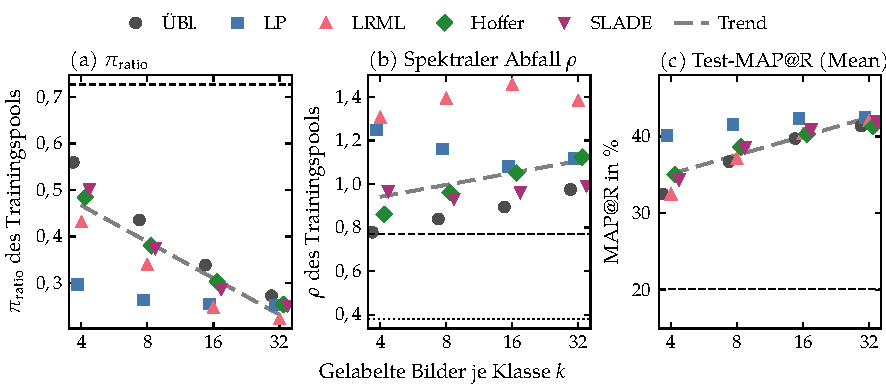
\includegraphics{neu/geometrie_budget}
  \caption[Geometrie des Embedding-Raums über das Label-Budget]{Geometrie des Trainingspools nach dem Training über das Label-Budget (Cars196, Seed~2, Mittel über die fünf Verlustfunktionen und die vier Folds). (a)~$\pi_{\mathrm{ratio}}$, (b)~spektraler Abfall $\rho$, (c)~Test-\acs{MAP@R} der Einzelmodelle. Schwarz gestrichelt: Head vor dem ersten Optimierungsschritt, gepunktet in (b): DINOv2-Merkmale. Grau gestrichelt: Trend über die fünf Verfahren (lineare Anpassung an ihren Median je Budget).}
  \label{fig:e:geo:budget}
\end{figure}

\ac{LP} erreicht schon bei $k=4$ fast dasselbe $\pi_{\mathrm{ratio}}$ wie die Referenz bei $k=32$ und eine Test-\ac{MAP@R} zwischen der Referenz bei $k=16$ und bei $k=32$. Unter den übrigen Verfahren ordnet $\pi_{\mathrm{ratio}}$ die Leistung bei $k=4$ dagegen nicht und auch der spektrale Abfall ordnet die Verfahren nicht nach ihrer Leistung. So erzeugt \ac{LRML} nach \ac{LP} die kompaktesten Klassen, erreicht bei $k=4$ aber nur die Test-\ac{MAP@R} der Referenz.%




\subsection{Verlauf über das Training}
\label{sec:e:verlauf}

Bei $k=4$ rücken unter der Referenz in der ersten Epoche alle Bilder innerhalb ihrer Klassen zusammen, danach entwickeln sich die gelabelten Bilder, die ungelabelten Bilder und die Validierungsklassen unterschiedlich. Bis Epoche~21, der im Mittel gewählten Epoche, werden nur die gelabelten Bilder weiter kompakter, bis auf ein $\pi_{\mathrm{intra}}$ von \num{0.17}, während die ungelabelten Bilder und die Validierungsklassen wieder stärker streuen. Der Head passt sich also an die wenigen gelabelten Bilder an und diese Anpassung überträgt sich nicht auf die übrigen Bilder derselben Klassen und auf ungesehene Klassen.%




Unter \ac{LP} werden dagegen auch die ungelabelten Bilder und die Validierungsklassen kompakter, sobald die Pseudo-Labels einsetzen. Mit ihnen steigen der Anteil ungelabelter Bilder mit richtigem Prototyp und die Validierungs-\ac{MAP@R} deutlich. Wie bei den Budgets der Phase~2 (Abschnitt~\ref{sec:e:nachbarschaft}) wird dabei auch der \ac{kNN}-Graph, aus dem \ac{LP} die Pseudo-Labels berechnet, mit jeder Verlustfunktion reiner. Mit ArcFace und Circle, deren Graphen 92 bzw.\ 38 Nachbarn haben, verlaufen am Ende des Warm-ups nur 39 bzw.\ \qty{58}{\percent} der Kanten innerhalb einer Klasse, die ersten Pseudo-Labels sind aber zu 66 bzw.\ \qty{78}{\percent} richtig. Mit \ac{MS}, \ac{NT-Xent} und Proxy-Anchor, deren Graphen 6 bis 7 Nachbarn haben, liegt die Kantenreinheit etwas über der Genauigkeit der ersten Pseudo-Labels.%


\ac{LRML}, Hoffer und \ac{SLADE} erreichen eine niedrigere Validierungs-\ac{MAP@R}. Mit diesen drei Mechanismen bleiben die ungelabelten Bilder weniger kompakt als mit \ac{LP}, am wenigsten mit Hoffer. Auch liegen weniger ungelabelte Bilder dem Prototyp ihrer Klasse am nächsten als mit \ac{LP}. Unter \ac{LRML} rücken die Klassenmittelpunkte nach dem Warm-up mit vier der fünf Verlustfunktionen zudem wieder zusammen, ebenso unter \ac{SLADE} mit Circle, unter \ac{LP} und Hoffer dagegen nicht. Der Graph von \ac{LRML} wird vor allem während des Warm-ups reiner (Tabelle~\ref{tab:a:reinheit:lrml}). Der spektrale Abfall steigt bei allen Verfahren im Laufe des Trainings, auch dort, wo die Validierungsleistung steigt. Er trennt die Überanpassung der Referenz damit nicht von einem nützlichen Training (Abbildung~\ref{fig:a:rho}). Bei $k=32$ streuen die ungelabelten Bilder unter der \UEBL nicht wieder stärker (Abbildung~\ref{fig:a:verlauf32}).%



\subsection{Semi-iNat-2021 und In-Shop}
\label{sec:e:geo:weitere}

\looseness=-1 Tabelle~\ref{tab:a:geometrie:weitere} in Anhang~\ref{chap:anhang:geometrie} zeigt die Geometrie auf Semi-iNat-2021 und beiden In-Shop-Serien. Auf Semi-iNat-2021 werden bei $k=2$ alle Verfahren außer \ac{LP} früh gewählt und unter der \UEBL, \ac{LRML}, Hoffer und \ac{SLADE} streuen die Klassen des Trainingspools stärker als vor dem Training ($\pi_{\mathrm{intra}}$ \num{0.66} bis \num{0.67} gegenüber \num{0.61}). Nur unter \ac{LP} werden sie kompakter (\num{0.58}) und \ac{LP} erreicht die höchste Test-\ac{MAP@R}. Auf In-Shop trennt dagegen jedes Training die Klassen deutlich. Dabei rücken die Klassenmittelpunkte auseinander. \ac{LP} und Hoffer ordnen dort die meisten ungelabelten Bilder dem richtigen Prototyp zu und erreichen die höchste Test-\ac{MAP@R}. In der Serie mit gelabelten Klassen machen \ac{LP} und \ac{SLADE} die ungelabelten Bilder kompakter als die \UEBL, rücken die Klassenmittelpunkte aber deutlich weniger auseinander. Bei 5 und \qty{10}{\percent} gelabelter Klassen hält \ac{LRML} die Mittelpunkte weiter auseinander und erreicht die höchste Test-\ac{MAP@R}, bei 25 und \qty{50}{\percent} liegen die \UEBL und Hoffer vorn. Auch auf diesen Datensätzen trifft die vorab festgelegte Erwartung nicht zu, beim kleinsten Budget hat der Head der \UEBL nirgends den größten spektralen Abfall.%


\subsection{Zusammenhang mit der Retrieval-Leistung}

\looseness=-1 Tabelle~\ref{tab:e:korrelation} setzt die Geometrie nach dem Training in Beziehung zur Test-\ac{MAP@R}, für jeden Datensatz über alle Kombinationen aus Verfahren, Verlustfunktion und Budget und innerhalb jedes Budgets. Auf Cars196 ist der Zusammenhang mit $\pi_{\mathrm{ratio}}$ des Trainingspools über alle 100 Kombinationen stark und negativ, mit einer Korrelation nach Pearson von \num{-0.86} und nach Spearman von \num{-0.80}. Innerhalb der Budgets wird er mit wachsendem $k$ schwächer und ist bei $k=32$ nur noch schwach (\num{-0.12}), weil dort $\pi_{\mathrm{intra}}$ und $\pi_{\mathrm{inter}}$ beide negativ mit der Test-\ac{MAP@R} zusammenhängen und sich im Verhältnis aufheben.

\begin{table}[tbp]
\centering\small\setlength{\tabcolsep}{4pt}
\caption[Korrelation der Geometrie mit der Retrieval-Leistung]{Rangkorrelation nach Spearman zwischen Maßen nach dem Training und der Test-MAP@R (Mean), Seed 2, Mittel über vier Folds. Gesamt: alle gültigen Kombinationen aus Verfahren, Verlustfunktion und Budget eines Datensatzes, darunter je Budget, Anzahl: Zahl dieser Kombinationen. In der In-Shop-Serie mit gelabelten Klassen steht der Anteil gelabelter Klassen für das Budget. Prototyp: Anteil der ungelabelten Bilder mit richtigem nächstem Klassenprototyp, in dieser Serie nicht definiert (--).}
\label{tab:e:korrelation}
\begin{tabular}{@{}l r S[table-format=-1.2] S[table-format=-1.2] S[table-format=-1.2] S[table-format=-1.2] @{\hspace{12pt}} S[table-format=-1.2] S[table-format=-1.2] S[table-format=-1.2] @{\hspace{12pt}} S[table-format=-1.2]@{}}
\toprule
& & \multicolumn{4}{c}{\textbf{Trainingspool}} & \multicolumn{3}{c}{\textbf{Validierungsklassen}} & {\textbf{Ungelabelt}} \\
\cmidrule(lr){3-6}\cmidrule(lr){7-9}\cmidrule(l){10-10}
& {Anzahl} & {$\pi_{\mathrm{intra}}$} & {$\pi_{\mathrm{inter}}$} & {$\pi_{\mathrm{ratio}}$} & {$\rho$} & {$\pi_{\mathrm{intra}}$} & {$\pi_{\mathrm{inter}}$} & {$\pi_{\mathrm{ratio}}$} & {Prototyp} \\
\midrule
\multicolumn{10}{@{}l}{\textbf{Cars196}} \\*
\quad \textit{gesamt} & 100 & -0.72 & 0.03 & -0.80 & 0.22 & -0.60 & 0.04 & -0.71 & 0.87 \\
\cmidrule{1-10}
\quad $k=4$ & 25 & -0.56 & 0.15 & -0.80 & 0.28 & -0.49 & 0.19 & -0.73 & 0.77 \\
\quad $k=8$ & 25 & -0.51 & 0.07 & -0.68 & 0.32 & -0.40 & 0.04 & -0.61 & 0.72 \\
\quad $k=16$ & 25 & -0.50 & -0.28 & -0.50 & 0.05 & -0.45 & -0.20 & -0.48 & 0.45 \\
\quad $k=32$ & 25 & -0.51 & -0.55 & -0.21 & -0.40 & -0.60 & -0.59 & -0.31 & 0.36 \\
\midrule
\multicolumn{10}{@{}l}{\textbf{Semi-iNat-2021}} \\*
\quad \textit{gesamt} & 100 & -0.80 & 0.14 & -0.80 & 0.74 & -0.69 & 0.12 & -0.51 & 0.95 \\
\cmidrule{1-10}
\quad $k=2$ & 25 & -0.23 & 0.17 & -0.09 & 0.13 & -0.24 & 0.24 & -0.12 & 0.17 \\
\quad $k=4$ & 25 & -0.14 & 0.27 & -0.19 & 0.23 & -0.09 & 0.24 & -0.13 & 0.35 \\
\quad $k=16$ & 25 & 0.24 & 0.10 & 0.41 & -0.63 & 0.20 & 0.03 & 0.46 & 0.69 \\
\quad $k=100$ & 25 & 0.42 & 0.25 & 0.33 & -0.45 & 0.46 & 0.21 & 0.37 & 0.84 \\
\midrule
\multicolumn{10}{@{}l}{\textbf{In-Shop}} \\*
\quad \textit{gesamt} & 50 & -0.10 & -0.03 & -0.37 & 0.21 & -0.04 & -0.05 & -0.31 & 0.89 \\
\cmidrule{1-10}
\quad $k=2$ & 25 & -0.11 & -0.12 & -0.32 & 0.55 & -0.04 & -0.18 & -0.23 & 0.94 \\
\quad $k=4$ & 25 & 0.38 & -0.17 & 0.45 & -0.17 & 0.37 & -0.17 & 0.45 & 0.67 \\
\midrule
\multicolumn{10}{@{}l}{\textbf{In-Shop mit gelabelten Klassen}} \\*
\quad \textit{gesamt} & 97 & -0.24 & 0.31 & -0.62 & 0.45 & -0.15 & 0.31 & -0.53 & {--} \\
\cmidrule{1-10}
\quad \qty{5}{\percent} & 25 & 0.06 & 0.13 & -0.12 & -0.02 & 0.08 & 0.13 & -0.10 & {--} \\
\quad \qty{10}{\percent} & 25 & 0.17 & 0.31 & -0.22 & 0.09 & 0.19 & 0.32 & -0.20 & {--} \\
\quad \qty{25}{\percent} & 24 & 0.66 & 0.63 & 0.13 & 0.05 & 0.69 & 0.61 & 0.17 & {--} \\
\quad \qty{50}{\percent} & 23 & 0.59 & 0.60 & 0.17 & -0.06 & 0.65 & 0.59 & 0.29 & {--} \\
\bottomrule
\end{tabular}
\end{table}


Mit dem spektralen Abfall besteht auf Cars196 kein linearer Zusammenhang. Am engsten hängt auf allen Datensätzen über alle Kombinationen die Genauigkeit der Prototypen-Zuordnung auf den ungelabelten Bildern mit der Test-\ac{MAP@R} zusammen (Tabelle~\ref{tab:e:korrelation}). Für diese Größe war vorab keine Erwartung festgelegt. Auf Semi-iNat-2021 und In-Shop hängt $\pi_{\mathrm{ratio}}$ über alle Budgets ebenfalls negativ mit der Test-\ac{MAP@R} zusammen, innerhalb der Budgets aber nur bei kleinem $k$. Auf Semi-iNat-2021 ist der Zusammenhang bei $k=2$ und 4 negativ (\num{-0.49} und \num{-0.41}), bei $k=16$ und 100 schwach positiv, auf In-Shop bei $k=2$ negativ und bei $k=4$ positiv. In der In-Shop-Serie mit gelabelten Klassen liegt er innerhalb der Anteile zwischen \num{-0.15} und \num{0.13}. Abschnitt~\ref{sec:d:ablationen} ordnet diese Zusammenhänge ein. Die Prototypen-Genauigkeit hängt dagegen in jedem Budget positiv mit der Test-\ac{MAP@R} zusammen, auf Semi-iNat-2021 mit \num{0.81} bis \num{0.89}. Auf Cars196 hängt bei kleinen Budgets zudem die Dauer des Trainings mit der Test-\ac{MAP@R} zusammen, mit einer Rangkorrelation zwischen gewählter Epoche und Test-\ac{MAP@R} von \num{0.61} bei $k=4$, bei $k=32$ nicht mehr.%




\section{Sensitivität der Hyperparameter, Rechenzeit und Speicherbedarf}
\label{sec:e:sensitivitaet}
\label{sec:e:aufwand}

Die Optima der Phase-1-Suchen sind flach. Im Median liegen 12 bis 48 der 80 Versuche einer Suche höchstens einen Prozentpunkt hinter dem besten und der zweitbeste Versuch nur \num{0.02} bis \num{0.13} Prozentpunkte dahinter. Innerhalb eines Standardfehlers der Fold-Werte des besten Versuchs liegen im Median auf \ac{CUB} 79 der 80 Versuche, auf Cars196 44, auf Semi-iNat-2021 25, auf In-Shop 6 und in der In-Shop-Serie mit gelabelten Klassen 4. Die exakten Werte einer gewählten Konfiguration sind deshalb nicht interpretierbar, nur der Bereich guter Werte. Auf den zufälligen Versuchen heben sich nur wenige Hyperparameter vom Rauschen ab, vor allem die Skalen von Proxy-Anchor, ArcFace und Circle, die Temperatur von \ac{NT-Xent} mit wechselndem Vorzeichen, die Distanzskala von Hoffer sowie das Warm-up und das Zielverhältnis $\eta$ von \ac{LRML} und $\eta$ von \ac{SLADE}. Die vier Parameter des Graphen und der Pseudo-Labels bei \ac{LP} heben sich nur in 10 ihrer 100 Kombinationen aus Parameter und Suche ab. Das schließt lokale Abhängigkeiten oder Wechselwirkungen nicht aus, wie die Einbrüche mit ArcFace auf In-Shop in den Sweeps zeigen.%


Die Mechanismen verlängern einen Trainingsschritt unterschiedlich stark, Hoffer am meisten. Auf In-Shop bei $k=2$ (Abschnitt~\ref{sec:m:aufwand}) dauert ein Schritt nach dem Warm-up mit der \UEBL \num{3.3} Millisekunden, mit \ac{LP} und \ac{LRML} \num{4.7} bzw.\ \num{6.3}, mit \ac{SLADE} \num{16.2} und mit Hoffer \num{24.8} Millisekunden. Eine Epoche einschließlich der Neuberechnung des Graphen, der Pseudo-Labels oder der Cluster und der Validierung dauert mit der \UEBL \num{0.6} Sekunden, mit \ac{LRML} \num{1.6}, mit \ac{LP} und \ac{SLADE} \num{2.6} bzw.\ \num{2.7} und mit Hoffer \num{3.9} Sekunden. Die Folds der Phase~1 trainieren dort im Median 155 bis 258 Epochen, am längsten mit der \UEBL und \ac{LP}. Mit diesen Epochen und den gemessenen Raten dauert ein Fold im Median \num{2.0}~Minuten mit der \UEBL, \num{3.4} mit \ac{LRML}, \num{6.8} mit \ac{SLADE}, \num{8.9} mit \ac{LP} und \num{10.4} mit Hoffer.%

Beim Speicherbedarf fällt nur \ac{NT-Xent} auf (Abschnitt~\ref{sec:m:verluste}). Ein Trainingsschritt belegt im Spitzenwert bei Batchgröße 256 und \ac{SPC}-4 rund \SI{0.7}{\giga\byte} zusätzlich, bei 512 und \ac{SPC}-2 rund \SI{1.8}{\giga\byte} und bei 512 und \ac{SPC}-8 rund \SI{12}{\giga\byte} (Abschnitt~\ref{sec:m:aufwand}). Die übrigen vier Verlustfunktionen bleiben bei dieser größten Kombination bei rund \SI{0.1}{\giga\byte} oder weniger.%

 % Cars196, CUB und In-Shop: gemeinsame Ergebnisdarstellung
\chapter{Diskussion}
\label{chap:diskussion}

Die Ergebnisse zeigen, dass ungelabelte Bilder das Retrieval auf ungesehenen Klassen auch gegenüber einer supervised Referenz (\UEBL) verbessern können, allerdings nur unter bestimmten Bedingungen und breit nur mit Label Propagation. Dieses Kapitel fragt deshalb weniger, welches Verfahren auf welchem Datensatz gewinnt, als unter welchen Bedingungen sich ungelabelte Bilder lohnen. Die Forschungsfragen und die Hypothesen werden dort beantwortet, wo die jeweilige Evidenz besprochen wird.



\section{Wann sich ungelabelte Bilder lohnen}
\label{sec:d:nutzen}

\subsection{Nutzen gegenüber einer abgestimmten Referenz}

Die erste Forschungsfrage (F1) lautete, ob ungelabelte Bilder die Retrieval-Leistung auf ungesehenen Testklassen gegenüber einer supervised Referenz verbessern. Die Antwort ist ein bedingtes Ja. Belastbar ist der Gewinn vor allem bei den Budgets, bei denen die Referenz und die Mechanismen abgestimmt wurden, auf Cars196 bei $k=16$ für \ac{LP} und auf In-Shop bei $k=2$ für \ac{LP} und Hoffer, die dort in keinem gepaarten Vergleich unter der Referenz liegen (Abschnitt~\ref{sec:e:phase1}). Den größten Gewinn erreicht \ac{LP} auf Cars196 bei vier gelabelten Bildern je Klasse. Im Mittel über die Verlustfunktionen ist die Richtung dieses Gewinns plausibel, denn um ihn aufzuheben, müsste eine für vier Labels je Klasse neu abgestimmte Referenz die bei $k=16$ abgestimmte Referenz mit viermal so vielen Labels übertreffen. Die Größe des Gewinns ist dagegen weder eine obere noch eine untere Schranke. Eine besser regularisierte Referenz könnte ihn verkleinern, ein für $k=4$ abgestimmtes \ac{LP} ihn vergrößern.%


In Trainingslabels ausgedrückt, bei derselben vollständig gelabelten Validierung in allen Budgets (Abschnitt~\ref{sec:budgets}), erreicht \ac{LP} auf Cars196 mit vier und mit acht gelabelten Bildern je Klasse im Mittel etwa die Leistung der Referenz mit der vierfachen Zahl, allerdings nur in ungepaarten Vergleichen innerhalb der gemessenen Budgets. Hypothese~H1 ist damit teilweise gestützt. Für \ac{LP} gilt sie auf Cars196 und Semi-iNat-2021 bis $k=16$ und auf In-Shop bei $k=2$ ohne einen negativen gepaarten Vergleich, für Hoffer, \ac{SLADE} und \ac{LRML} nur auf einzelnen Datensätzen (Abschnitt~\ref{sec:e:phase1}). Auf \ac{CUB} ist sie nur für das Ensemble mit wenigen Zehnteln eines Prozentpunkts gestützt.%


Mit früheren Arbeiten zum \ac{SSDML} lassen sich diese Gewinne nur bedingt vergleichen. Auf \ac{CUB} steigt in einer davon mit fünf Labels je Klasse die \ac{P@1}, dort als Recall@1 berichtet, von \qty{31.7}{\percent} vor dem Training auf \qty{44.8}{\percent}, aber nur um \num{2.2} bis \num{3.4} Prozentpunkte über supervised Baselines mit denselben Labels~\cite{dutta_semi-supervised_2021}. Label Propagation mit proxybasierten Ankern wird auf einer eigenen Aufteilung der Klassen gegen supervised Verfahren mit Standard-Hyperparametern verglichen und liegt in der \ac{NMI} auf Cars196 um 2,6 und auf \ac{CUB} um 4,4 Punkte über dem besten von ihnen~\cite{zhuang_deep_2021}. Die gemischte Label Propagation der Folgearbeit liegt dort um 2,6 und 4,5 Punkte darüber~\cite{zhuang_deep_2023}. Alle drei Arbeiten trainieren ein vortrainiertes \ac{CNN} mit und berichten keine \ac{MAP@R}. Diese berichten \ac{SLADE} und \ac{STML}, beide aber mit allen Labels und zusätzlichen externen Bildern~\cite{duan_slade_2021, kim_self-taught_2022}. \ac{SLADE} übertrifft den eigenen Teacher mit derselben Verlustfunktion auf \ac{CUB} um \num{4.3} bis \num{4.7} und auf Cars196 um \num{3.7} bis \num{5.4} Prozentpunkte~\cite{duan_slade_2021}. \ac{STML} liegt mit einem auf ImageNet vortrainierten ResNet50 und 512 Dimensionen auf \ac{CUB} um \num{11.4} und auf Cars196 um \num{10.1} Prozentpunkte über dem supervised Modell mit \ac{MS}, von dem es ausgeht~\cite{kim_self-taught_2022}. In dieser Arbeit entfällt auf Cars196 und In-Shop ebenfalls der größere Teil des Sprungs von den unveränderten Merkmalen auf das supervised Training, auf Cars196 bei $k=4$ gut zwölf Prozentpunkte gegenüber weiteren \num{7.8} durch \ac{LP} (Tabelle~\ref{tab:e:referenz}, Abbildung~\ref{fig:e:gewinne}). Ein Gewinn gegenüber unveränderten Merkmalen oder nicht abgestimmten Baselines sagt damit wenig über den Nutzen ungelabelter Bilder aus. Auch in der Klassifikation schrumpften die berichteten Gewinne, sobald die supervised Baseline gleich intensiv abgestimmt wurde~\cite{oliver_realistic_2018} (Abschnitt~\ref{sec:ssl:evaluation}).

\subsection{Messbarer und praktisch bedeutsamer Gewinn}

Ob ein Gewinn messbar ist und ob er lohnenswert ist, ist nicht dasselbe. Auf Semi-iNat-2021 ist der Gewinn von \ac{LP} bei zwei Labels je Art kein Zufall der Seeds, entspricht aber nur dem Schritt der Referenz von zwei auf vier Labels je Art. Allerdings brächten dort auch zusätzliche echte Labels vergleichsweise wenig (Abschnitt~\ref{sec:e:ausgangslage}). Auf \ac{CUB} übertreffen schon die unveränderten DINOv2-Merkmale die meisten trainierten Einzelmodelle (Abschnitt~\ref{sec:e:ausgangslage}) und kein Mechanismus hat diesen Rückstand in einen nennenswerten Gewinn verwandelt. Auch beim Fine-Tuning des ganzen DINOv2 war \ac{CUB} unter mehreren Retrieval-Datensätzen der einzige, auf dem das unveränderte Modell kaum zurücklag~\cite{berton_all_2025}. Ebenso war \ac{CUB} unter den drei Datensätzen von ooDML der einzige, auf dem die unveränderten Merkmale eines vortrainierten ResNet (BiT) in der Recall@1 vor den dort trainierten \ac{DML}-Modellen lagen~\cite{milbich_characterizing_2021}.

Wie zu erwarten, fallen die Gewinne dort groß aus, wo auch zusätzliche echte Labels die Referenz noch deutlich verbessern. Der stärkste Gewinn wird auf Cars196 gemessen und der kleinste Gewinn auf \ac{CUB}. Das ist plausibel für Mechanismen, die Pseudo-Labels wie echte Labels verwenden, denn im günstigsten Fall wirkt jedes ihrer Pseudo-Labels wie ein echtes Label für dasselbe Bild. Den verbleibenden Spielraum zeigt die Referenz mit allen Labels der Trainingsklassen, die auf \ac{CUB} und Semi-iNat-2021 kaum, auf Cars196 und In-Shop dagegen noch über dem größten Budget liegt (Abschnitt~\ref{sec:e:ausgangslage}). Für einen Term wie den von \ac{LRML} ist das keine feste Grenze, denn auf Cars196 liegt \ac{LRML} auch mit allen Labels und ohne ungelabelte Bilder über der \UEBL (Abschnitt~\ref{sec:e:extern}). Mit vier Datensätzen ist dieser Zusammenhang eine Beobachtung. Der verbleibende Spielraum ist keine hinreichende Bedingung für einen Gewinn. Auf Semi-iNat-2021 gewinnt die Referenz von $k=2$ bis zu allen Labels noch rund drei Prozentpunkte, \ac{LP} bei $k=2$ aber nur \num{0.6}. In der In-Shop-Serie mit vollständig gelabelten Klassen gewinnt die Referenz mit mehr gelabelten Klassen ebenfalls deutlich, während \ac{LP} trotzdem verliert (Abschnitt~\ref{sec:d:daten}).
 

Die Auswahl der Vortrainingsdaten erklärt dieses Muster nicht allein (Abschnitt~\ref{sec:vit}). In dieser Arbeit bleibt trotzdem auf Cars196 der größte und auf Semi-iNat-2021 ein kleiner Spielraum. Für \ac{CUB} und Cars196 kommt als weitere Erklärung der Abstand zwischen Trainings- und Testklassen in Frage (Abschnitt~\ref{sec:modellauswahl}). Gemessen am Spektrum der ooDML-Aufteilungen liegt er in der üblichen Aufteilung von Cars196 nahe am Wert einer zufälligen Aufteilung der Bilder derselben Klassen, bei \ac{CUB} deutlich darüber. Für diese Arbeit folgt daraus nur die Hypothese, dass sich das auf den Trainingsklassen Gelernte auf Cars196 leichter auf die Testklassen überträgt als auf \ac{CUB}, denn der Abstand wurde mit ResNet50- und nicht mit DINOv2-Merkmalen gemessen \cite{milbich_characterizing_2021}. Auf Cars196 finden die unveränderten Merkmale meist ein Bild desselben Modells als ersten Treffer, ordnen die übrigen Bilder der Klasse aber nicht zusammen (Abschnitt~\ref{sec:e:ausgangslage}). Nach dem vollständigen Fine-Tuning eines auf ImageNet-21k vortrainierten ViT-S/16 mit Proxy-Anchor und allen Labels erreicht ein Modell auf Cars196 eine \ac{P@1}, als Recall@1 berichtet, von \qty{86.7}{\percent}, aber nur eine \ac{MAP@R} von \qty{28.7}{\percent}, auf \ac{CUB} bei ähnlicher \ac{P@1} dagegen \qty{51.1}{\percent}~\cite{ren_learning_2024}. Eine feste Eigenschaft von Cars196 ist das aber nicht, denn nach dem Fine-Tuning des ganzen DINOv2-B erreichen dort zehn von zwölf Verlustfunktionen bei Batchgröße 256 eine \ac{MAP@R} von rund \qty{54}{\percent} bis \qty{57}{\percent}, ähnlich wie auf \ac{CUB}~\cite{berton_all_2025}. Auch der lineare Klassifikationsvergleich aus Abschnitt~\ref{sec:vit} spricht dafür, dass die Merkmale die Klassen unterscheiden können. Im Beispiel aus Abbildung~\ref{fig:e:retrieval} folgt die Ähnlichkeit auf Cars196 aber auch der Farbe und der Größenklasse, während eine Klasse dasselbe Modell in jeder Farbe umfasst. Gerade die Lücke zwischen dem nächsten Nachbarn und der ganzen Klasse ist der Raum, den ein Head und mit ihm die Pseudo-Labels füllen können. Für \ac{SSL} mit vortrainierten Modellen eignen sich in der Klassifikation deshalb vor allem Aufgaben, bei denen eingefrorene Merkmale noch Spielraum lassen, denn verbreitete Benchmarks bieten kaum noch welchen~\cite{zhang_revisiting_2025}. Die Vermutung aus der Einleitung, dass ein großer Teil des möglichen Beitrags ungelabelter Bilder bereits im Vortraining steckt, trifft damit eher auf \ac{CUB} und Semi-iNat-2021 zu als auf Cars196 und In-Shop bei kleinen Budgets. Schwache Merkmale allein sichern allerdings keinen großen Gewinn. Auf In-Shop sind die unveränderten Merkmale viel schwächer als auf Cars196, der größte Gewinn fällt aber kleiner aus (Abschnitt~\ref{sec:e:phase1}). Das könnte daran liegen, dass auf In-Shop beim kleinsten Budget schon rund \qty{31}{\percent} des Pools gelabelt sind, auf Cars196 nur \qty{4.9}{\percent} (Abschnitt~\ref{sec:budgets}). Zudem gewinnt die Referenz auf In-Shop bis zu allen Labels weniger hinzu (Tabelle~\ref{tab:e:referenz}).

Für \ac{CUB} liegt eine Erklärung in der hohen Ausgangsleistung auf den Validierungsfolds nahe (Abschnitt~\ref{sec:e:ausgangslage}). Wenn auf den Trainingsklassen ähnlich wenig zu ordnen bleibt, liefern die Labels dem Verlust kaum etwas, das die Merkmale nicht schon enthalten, was auch erklären würde, warum zusätzliche echte Labels die \UEBL dort kaum verbessern. Auf den Trainingsklassen selbst wurde das nicht gemessen. An der Auswahl zwischen den 100 Kombinationen liegt es vermutlich nicht, denn die Validierung trennt sie über dem Rauschen der Seeds und auch die im Test beste Kombination liegt kaum über den Merkmalen. Offen bleibt die Wahl der Epoche, weil auf \ac{CUB} nur das gewählte Modell getestet wird. Auf Semi-iNat-2021 spricht die ähnlich hohe \ac{P@1} vor dem Training für dieselbe Erklärung, die deutlich niedrigere Validierungs-\ac{MAP@R} dagegen.

\subsection{Label-Budget, Verlustfunktion und Aggregation}

Die zweite Forschungsfrage (F2) erfragte im ersten Teil, wie der Nutzen von dem Label-Budget, von dem Datensatz und von der Verlustfunktion abhängt. Vom Datensatz hängt er über den verbleibenden Spielraum ab, soweit vier Datensätze das erkennen lassen. Innerhalb eines Datensatzes sinkt der Gewinn der Verfahren, die bei kleinem Budget gewinnen, mit dem Budget. Der Gewinn von \ac{LRML} als Einzelmodell bleibt auf Cars196 etwa gleich (Abschnitt~\ref{sec:e:faktoren}). H2 ist damit als Muster teilweise gestützt. Das entspricht der Erwartung aus Abschnitt~\ref{sec:einordnung}, die sich auf Befunde der semi-supervised Klassifikation stützt~\cite{oliver_realistic_2018}. Frühere Arbeiten zum \ac{SSDML} erlauben hier dagegen keinen Vergleich, denn sie untersuchen je Datensatz nur ein Budget, wie fünf Labels je Klasse~\cite{dutta_semi-supervised_2021, zhuang_deep_2021, zhuang_deep_2023} oder alle Labels mit einem externen ungelabelten Datensatz~\cite{duan_slade_2021}. In dieser Arbeit bleibt die Ursache des Rückgangs offen, denn mit dem Budget ändern sich zugleich das Verhältnis ungelabelter zu gelabelten Bildern, die Stärke der Referenz und der Abstand zu dem Budget, bei dem die Hyperparameter gesucht wurden. Über einen Rückgang hinaus geht die Umkehr von \ac{LP} auf Semi-iNat-2021 bei $k=100$ (Abschnitt~\ref{sec:e:phase1}). Sie passt zum verbleibenden Spielraum, denn zusätzliche echte Labels bringen der Referenz dort nichts mehr (Tabelle~\ref{tab:e:referenz}), sodass selbst überwiegend richtige Pseudo-Labels vor allem durch ihre Fehler wirken könnten.%


Für das supervised \ac{DML} wurde gezeigt, dass sich Verlustfunktionen unter einheitlichen Versuchsbedingungen nur wenig unterscheiden~\cite{musgrave_metric_2020, roth_revisiting_2020}. Auch beim Fine-Tuning des ganzen DINOv2 liegen die Ergebnisse der Verlustfunktionen in einem Vergleich verschiedener Batchgrößen auf Cars196 und \ac{CUB} nahe beieinander~\cite{berton_all_2025}. Für den Nutzen eines Mechanismus kann die Verlustfunktion dagegen entscheidend sein. Auf Cars196, In-Shop und Semi-iNat-2021 liegt \ac{LP} bei kleinen Budgets als Einzelmodell mit jeder Verlustfunktion über der \UEBL, während bei \ac{LRML}, Hoffer und \ac{SLADE} schon das Vorzeichen des Gewinns von der Verlustfunktion abhängen kann (Abschnitt~\ref{sec:e:beste}). Dazu passt, dass \ac{LP} auf Cars196 bei jedem Budget mit \ac{MS} vorn liegt, der Verlustfunktion, die auch für die \UEBL meist am besten ist (Abschnitt~\ref{sec:e:beste}). Die Beiträge des Verfahrens und der Verlustfunktion scheinen sich dort zu addieren. Das passt dazu, dass \ac{LP} die Pseudo-Labels wie echte Labels an die Verlustfunktion übergibt, sodass kein zusätzlicher Term gegen den supervised Verlust abgewogen werden muss. Für die Bewertung eines Mechanismus mit eigenem Term genügt deshalb eine einzelne Verlustfunktion nicht, denn mit \ac{MS} verliert \ac{LRML} auf Cars196 bei $k=4$, mit den übrigen vier gewinnt es (Abbildung~\ref{fig:e:verluste}). Eine mögliche Erklärung liegt in der Gewichtung dieser Terme. Ihr Gewicht folgt einem Zielverhältnis zu einer Statistik der supervised Gradienten (Abschnitt~\ref{sec:m:gewicht}) und wie stark diese Gradienten auf wenige Parameter konzentriert sind, könnte von der Skala und der Temperatur der Verlustfunktion abhängen. Dasselbe $\eta$ würde dann je nach Verlustfunktion eine andere wirksame Stärke bedeuten. Dafür spricht, dass die Leistung von \ac{LRML} auf In-Shop mit Circle schon ab $\eta=\num{0.75}$ einbricht, mit Proxy-Anchor erst bei $\eta=3$ (Abschnitt~\ref{sec:e:sweeps}), gemessen wurde die wirksame Stärke aber nicht. Für die Praxis folgt daraus, dass sich die Konfiguration eines zusätzlichen Terms nicht ohne neue Suche von einer Verlustfunktion auf eine andere übertragen lässt. Eine Gewichtung, die das Verhältnis der euklidischen Gradientennormen laufend verfolgt, statt es nur zu Beginn zur Kalibrierung zu nutzen (Abschnitt~\ref{sec:m:gewicht}), könnte diese Abhängigkeit verringern und damit auch die Ergebnisse von \ac{LRML}, Hoffer und \ac{SLADE} verbessern.

Wie ein Gewinn zu bewerten ist, hängt außerdem davon ab, ob ein Einzelmodell oder ein Ensemble der Fold-Modelle eingesetzt wird. Bei \ac{LRML} auf Cars196 ist der Gewinn bei kleinen Budgets im Ensemble ein Mehrfaches des Gewinns als Einzelmodell, denn seine Fold-Modelle irren sich seltener gleich (Abschnitt~\ref{sec:e:phase2:concat}). Ein Mechanismus kann also vor allem die Vielfalt der Fold-Modelle erhöhen. Wer nur ein einzelnes Modell einsetzen kann, hat von diesem Vorteil nichts. Die Dimension der Embeddings im Index wächst mit der Zahl der Fold-Modelle, hier auf das Vierfache und auf \ac{CUB} auf das Fünffache (Abschnitt~\ref{sec:protokoll}).%

\section{Welche ungelabelten Daten ein Gewinn voraussetzt}
\label{sec:d:daten}

Neben dem Verfahren und der Verlustfunktion spielt auch die Zusammensetzung der ungelabelten Daten eine Rolle. In der In-Shop-Serie mit vollständig gelabelten Klassen stammen sie ausschließlich aus Klassen ohne Label. Externe Bildmengen wie in der Originalarbeit von \ac{SLADE} (Abschnitt~\ref{sec:ssdml}) prüft ein eigener Versuch (Abschnitt~\ref{sec:d:extern}).

\subsection{Bilder aus Klassen ohne Labels}

Die deutlichste Voraussetzung betrifft die Klassen. \ac{LP} und Hoffer ordnen jedes ungelabelte Bild einer gelabelten Klasse zu. Stammen die ungelabelten Bilder aus Klassen ohne Label, ist jede solche Zuordnung falsch und \ac{LP} ist in der In-Shop-Serie im Mittel über die Verlustfunktionen bei jedem Anteil gelabelter Klassen schlechter als die Referenz. Die Konfidenz erkennt Bilder neuer Klassen nicht, denn sie misst nur, wie stark sich die Score-Masse eines Bildes auf wenige bekannte Klassen konzentriert (Abschnitt~\ref{sec:lp}). Wie sehr die falschen Pseudo-Labels schaden, hängt aber von der Verlustfunktion ab. ArcFace und Proxy-Anchor, mit denen \ac{LP} am meisten verliert, ziehen jedes Bild zum Proxy seiner Klasse und damit Bilder neuer Klassen in eine fremde Klasse (Abschnitt~\ref{sec:verluste:proxy}). Paarbasierte Verlustfunktionen prüfen dagegen nur, ob zwei Bilder dasselbe Label tragen, sodass Bilder eines neuen Artikels mit demselben falschen Label trotzdem richtige positive Paare bilden können. Mit ArcFace, Proxy-Anchor und, gegen diese Erklärung, auch mit Circle erholt sich die Validierung nach den ersten Pseudo-Labels meist nicht mehr. Weil die Modellauswahl nach dem Warm-up neu beginnt (Abschnitt~\ref{sec:m:ssl}), kann \ac{LP} dann nicht auf das bessere Modell davor zurückfallen. H3 ist damit für \ac{LP} in der hier verwendeten Form gestützt. Ob eine absolute Konfidenzschwelle oder die mit der Konfidenz gewichtete Kreuzentropie des Originalverfahrens~\cite{iscen_label_2019} den Schaden begrenzen würde, wurde nicht untersucht. Für Hoffer ist H3 nur schwach gestützt, weil dessen Ergebnis über alle Anteile nahe null bleibt und nicht erkennbar ist, ob der Term dort wirkungslos ist oder den Bildern neuer Klassen standhält. Für \ac{SLADE}, das schon in der $k$-Serie auf In-Shop nicht gewinnt, lässt sich H3 hierdurch nicht prüfen.

Eine erwartete Ausnahme für Mechanismen ohne Zuordnung zu einer bekannten Klasse zeigt sich nur teilweise. \ac{LRML} gewinnt im Ensemble nur bei kleinen Anteilen gelabelter Klassen, mit Circle aber bei jedem Anteil (Abschnitt~\ref{sec:e:klassen}). Bei \qty{10}{\percent} gelabelter Klassen geht dieser Gewinn zum größten Teil auf die ungelabelten Bilder zurück (Tabelle~\ref{tab:e:klassen:2x2}). Ob dabei die Herkunft oder die Menge der ungelabelten Bilder entscheidet, trennt die Serie nicht, denn der ungelabelte Pool ist gerade bei den kleinen Anteilen am größten.

Für die semi-supervised Klassifikation wurde berichtet, dass Klassen, die nur im ungelabelten Pool vorkommen, die Leistung verschlechtern können~\cite{oliver_realistic_2018}. Dort wurden die Hyperparameter dafür nicht neu gesucht. Hier wurden die Hyperparameter dagegen eigens für die Serie mit \qty{10}{\percent} gelabelter Klassen gesucht (Abschnitt~\ref{sec:budgets}, Tabelle~\ref{tab:inshop10:hpo}). Die In-Shop-Serie dieser Arbeit deutet für das \ac{DML} an, dass der Schaden von der Art des Mechanismus abhängen könnte. Diese mögliche Abhängigkeit vom Mechanismus passt zu den kontrollierten Klassifikationsversuchen aus Abschnitt~\ref{sec:ssl:evaluation}. Die bereits beschriebenen Befunde zu Hoffer und \ac{SLADE} erlauben keine eindeutige Trennung nach dem Zuordnungsprinzip. Zudem beruht der Vergleich auf einem Datensatz und zwei Serien.

\subsection{Externe ungelabelte Bilder}
\label{sec:d:extern}

Für \ac{SLADE} wurde mit allen Labels und einem externen ungelabelten Datensatz ein deutlicher Gewinn gegenüber dem Teacher berichtet, auf Cars196 mit CompCars als externem Datensatz~\cite{duan_slade_2021}. In dieser Arbeit liegt unter ähnlichen Bedingungen kein Mechanismus über der \UEBL, auch die angepasste Variante von \ac{SLADE} nicht (Abschnitt~\ref{sec:e:extern}). Die Bedingungen unterscheiden sich aber, denn das Backbone ist hier eingefroren, die Referenz ist die \UEBL statt des Teachers (Abschnitt~\ref{sec:d:nutzen}) und die Cluster stammen vom trainierten Head selbst (Abschnitt~\ref{sec:m:slade}).

Für den Verlust kommen mehrere Gründe in Frage. Die Konfigurationen wurden für wenige Labels und den internen Pool gesucht und unverändert übernommen. Der Mechanismus kann bei vollständigen Labels auch ohne ungeeignete Bilder schaden. Die externen Bilder können zudem schaden, weil sie zu anderen Klassen gehören oder anders aussehen. Dass der Verlust bei \ac{LP}, Hoffer und \ac{SLADE} auf Cars196 schon mit \qty{10}{\percent} von CompCars voll auftritt und mit dem Pool kaum wächst, spricht zudem für einen Grund im Aufbau des Trainings. Bei \ac{LP} stammen auf Cars196 nur 12,5 bis \qty{25}{\percent} jedes Batches aus den gelabelten Bildern und der Rest aus pseudo-gelabelten Bildern, unabhängig von der Größe des Pools (Abschnitte~\ref{sec:m:lp} und~\ref{sec:e:extern}). Bei Hoffer und \ac{SLADE} legt das Zielverhältnis das Gewicht des Terms fest, ebenfalls unabhängig vom Pool (Abschnitt~\ref{sec:m:gewicht}). 

Bei \ac{LRML} läuft der Term in der Kontrolle weiter, auf Cars196 entsteht sein Leistungsverlust also erst durch die externen Bilder. Auf In-Shop liegen die Kontrollen im Mittel unter der \UEBL, sodass dort auch die übernommenen Konfigurationen als Grund in Frage kommen. Bei \ac{LP} gilt das aber nur für ArcFace. Mit den übrigen vier Verlustfunktionen liegt seine Kontrolle über der \UEBL und der Verlust entsteht erst mit den externen Bildern (Abschnitt~\ref{sec:e:extern}). Dazu passt die Art dieser Bilder. Da jede Klasse ein einzelner Artikel ist, dürfte kaum ein Bild aus Fashion200k zu einer gelabelten Klasse gehören, zudem sind die Bilder von Fashion200k anders als die von In-Shop zugeschnitten (Abschnitt~\ref{sec:daten}). Für \ac{LP} gleicht die Lage dann der In-Shop-Serie mit vollständig gelabelten Klassen, in der jedes Pseudo-Label falsch ist (Abschnitt~\ref{sec:d:daten}). Dass andere Nachbar- und Clusterzahlen die Verluste auf Cars196 nicht aufheben (Abschnitt~\ref{sec:e:extern}), spricht gegen diese beiden Werte als Ursache, schließt eine unpassende Konfiguration aber nicht aus, weil für dieses Setting keine vollständige \ac{HPO} durchgeführt wurde.%





\subsection{Nachbarschaften und Klassengröße}

Innerhalb der gelabelten Klassen hängt der Nutzen davon ab, wie gut die Nachbarschaften im Embedding-Raum des Heads die Klassen wiedergeben. Auffällig ist dabei, wie wenig reine Nachbarschaften \ac{LP} mit großen Graphen braucht. Bei $k=4$ liegt auf Cars196 nur mit 38 und 92 Nachbarn die Genauigkeit der ersten Pseudo-Labels über dem Anteil der Kanten innerhalb einer Klasse (Abschnitt~\ref{sec:e:verlauf}). Das spricht dafür, dass ein Pseudo-Label bei großen Graphen der Mehrheit vieler Pfade und nicht einzelnen Kanten folgt. Die Smoothness- und die Cluster-Annahme müssten für \ac{LP} dann nicht für jede Kante gelten, sondern nur für die Klassen als Ganzes. Für die offene Frage aus der Einleitung nach den Annahmen über die Struktur der Daten wäre das nur eine teilweise Antwort, denn sie gilt für die Trainingsklassen von Cars196 im Embedding-Raum nach dem Warm-up. Dass der Anteil gleichklassiger Kanten während des Trainings mit \ac{LP} steigt, ist allerdings kein unabhängiger Beleg dafür, dass diese Annahmen im Embedding-Raum zunehmend gelten, denn \ac{LP} trainiert den Head gerade mit den Labels, die aus diesem Graphen stammen. Wie sehr dabei die Ausgangsmerkmale zählen, deutet ein Vergleich an. Mit den Merkmalen eines vortrainierten BN-Inception und fünf Labels je Klasse ordnet Label Propagation auf ganz Cars196 nur rund ein Fünftel der Bilder richtig zu~\cite{zhuang_deep_2023}. Hier sind bei $k=4$ schon die ersten Pseudo-Labels mit ArcFace und Circle zu \qty{66}{\percent} bzw.\ \qty{78}{\percent} richtig (Abschnitt~\ref{sec:e:verlauf}). Diese Anteile beziehen sich allerdings nur auf die übernommenen Pseudo-Labels über der Konfidenzschwelle.

Für \ac{LRML} gilt diese Mehrheitsentscheidung nicht, denn der Term zieht jede gezogene Kante einzeln zusammen. Die beste Nachbarzahl könnte deshalb von der Klassengröße abhängen. Auf In-Shop mit wenigen Bildern je Klasse sind die kleinsten Nachbarzahlen am besten und reinere Kanten helfen deutlich, auf Cars196 mit vielen Bildern je Klasse liegen viele Nachbarzahlen gleichauf und reinere Kanten helfen kaum (Abschnitt~\ref{sec:e:sweeps}, Tabelle~\ref{tab:e:ablationen:verluste}). Bei wenigen Bildern je Klasse verlassen schon wenige Nachbarn die Klasse und der Term erzwingt Nähe genau dort, wo die Labels wechseln. Die Zahl der Bilder je Klasse im Pool könnte damit eine Größe sein, nach der sich die Nachbarzahl ohne Labels wählen lässt, sofern die ungefähre Klassengröße bekannt ist. Auf Cars196 wirkt der Term dagegen auf andere Weise (Abschnitt~\ref{sec:d:ablationen}). Dieselbe Schwierigkeit ist für ein graphbasiertes Verfahren beschrieben, das negative Paare über eine Nachbarzahl bestimmt, besonders bei unausgeglichenen Klassen~\cite{zhuang_deep_2023}. In dieser Arbeit gewinnt \ac{LRML} auf Semi-iNat-2021 nicht, dessen Arten im Mittel rund 150, aber sehr unterschiedlich viele Bilder haben (Abschnitt~\ref{sec:budgets}). Dort könnte keine einzelne Nachbarzahl zu großen und kleinen Arten zugleich passen.

\section{Was die Ablationen erklären}
\label{sec:d:ablationen}

Für F2 sollte außerdem geklärt werden, worauf ein Gewinn beruht. Die separat abgestimmten Hyperparameter allein erzeugen ihn nicht (Abschnitt~\ref{sec:e:2x2}). Die Kontrolle mit abgeschaltetem \ac{SSL}-Term liegt in 25 der 40 Kombinationen sogar um mehr als die Rauschschwelle unter der \UEBL, nicht wie erwartet auf ihrem Niveau. Das spricht dafür, dass die Suche die Hyperparameter auf den jeweiligen Mechanismus abstimmt. Der Vergleich mit dieser Kontrolle zeigt deshalb nur, was der Term innerhalb seiner Konfiguration bewirkt, nicht schon einen Gewinn gegenüber der \UEBL. Wie unsicher ein Urteil mit einem Seed ist, zeigt die Zerlegung selbst, denn sechs der 14 Kombinationen ohne Gewinn liegen im Mittel der fünf Seeds der Phase~1 über der \UEBL (Abschnitt~\ref{sec:e:2x2}).

\subsection{Ursachen je Mechanismus}

Für \ac{LP} ist die Zerlegung am klarsten. Der Mechanismus bewirkt allein auf den gelabelten Bildern fast nie etwas und sein Gewinn bleibt mit den gemeinsamen Hyperparametern der Referenz meist bestehen (Abschnitt~\ref{sec:e:2x2}). Er beruht also auf den ungelabelten Bildern und, wie der umverdrahtete Graph zeigt (Abschnitt~\ref{sec:e:nachbarschaft}), auf ihrer Nachbarschaft. Dass es auf die aus den Daten berechnete Nachbarschaft ankommt, passt zur Klassifikation, wo der Vergleich von Pseudo-Labels aus dem Graphen und aus den Vorhersagen des Netzes zugunsten des Graphen ausfällt~\cite{iscen_label_2019}.%


Bei \ac{LRML} ist der Gewinn auf Cars196 nur zum Teil ein Gewinn durch ungelabelte Bilder. Schon auf den gelabelten Bildern hebt der Term die Leistung mit allen fünf Verlustfunktionen über die Kontrolle mit abgeschaltetem Term. Klassenreine Nachbarschaften erklären diesen Beitrag nicht. Die in Abschnitt~\ref{sec:e:2x2} hergeleitete Mehrheit klassenübergreifender Nachbarschaftsbeziehungen in dieser Variante spricht gegen eine Erklärung allein durch klassenreine Kanten. Zudem helfen reinere Kanten \ac{LRML} auf Cars196 kaum. Ein zufälliger Graph schadet dagegen. Das spricht dafür, dass der Term dort weniger die Klassenstruktur überträgt, als vielmehr als datenabhängige Glättung wirkt, die benachbarte Merkmale ähnlich abbildet. Das entspricht der Idee der Mannigfaltigkeitsregularisierung, die mit einem datenabhängigen Term Funktionen bevorzugt, die entlang der Datenverteilung glatt sind~\cite{belkin_manifold_2006}. Auf In-Shop und im Ensemble tragen dagegen vor allem die ungelabelten Bilder bei (Abschnitte~\ref{sec:e:2x2} und~\ref{sec:e:phase2:concat}).%


Bei Hoffer stammt der Gewinn vor allem aus den ungelabelten Bildern. Auf In-Shop hebt aber auch der Term auf den gelabelten Bildern allein die Leistung. Mit den gemeinsamen Hyperparametern der Referenz gewinnt Hoffer auf In-Shop, auf Cars196 nicht (Abschnitt~\ref{sec:e:2x2}). Ob das Ausbleiben auf Cars196 eine echte Abhängigkeit von der übrigen Konfiguration anzeigt oder nur eine unpassende Kombination übertragener Werte, trennen die Versuche nicht.%


Bei \ac{SLADE} zeigen die Ablationen, dass die ungelabelten Bilder auf In-Shop kaum etwas beitragen (Abschnitt~\ref{sec:e:2x2}), aber nicht, warum. Weder die eigenen noch die Hyperparameter der \UEBL führen dort zu einem Gewinn und kein Wert der Sweeps verbessert das Ergebnis deutlich (Abschnitte~\ref{sec:e:2x2} und~\ref{sec:e:sweeps}). Andere gemeinsame Einstellungen mehrerer Hyperparameter sind damit nicht ausgeschlossen. Eine mögliche Erklärung liegt in den sicheren Paaren, die \ac{SLADE} aus Clustern ohne Bezug zu den gelabelten Klassen bildet. Bei wenigen Bildern je Artikel könnten viele dieser Paare verschiedene Artikel verbinden, so wie bei \ac{LRML} auf In-Shop schon wenige Nachbarn die Klasse verlassen (Abschnitt~\ref{sec:d:daten}). Auch im Original erreicht \ac{SLADE} auf In-Shop nur das Niveau supervised trainierter Verfahren~\cite{duan_slade_2021}. Auf Cars196 gewinnt die hier verwendete Form ohne getrennten Teacher dagegen bei kleinen Budgets.%


\subsection{Falsche Pseudo-Labels}

Die Genauigkeit der Pseudo-Labels allein ist ein unzureichendes Maß für ihren Nutzen. Bei ähnlich genauen ersten Pseudo-Labels gewinnt \ac{LP} bei $k=2$ auf In-Shop ein Mehrfaches des Gewinns auf Semi-iNat-2021 (Abschnitt~\ref{sec:e:pseudolabels}). Zum Teil passt das dazu, dass echte Labels die Referenz von $k=2$ bis zu allen Labels auf Semi-iNat-2021 nur etwa halb so stark verbessern wie auf In-Shop (Tabelle~\ref{tab:e:referenz}). Der Unterschied der Gewinne ist aber deutlich größer. Auf Semi-iNat-2021 liegt \ac{LP} bei hundert Labels je Art sogar trotz überwiegend richtiger Pseudo-Labels in allen Vergleichen unter der Referenz (Abschnitt~\ref{sec:e:pseudolabels}). Gegenüber den Oracle-Varianten liegt reguläres \ac{LP} meist über der Kurve zufälliger Fehler gleicher Häufigkeit (Abschnitt~\ref{sec:e:pseudolabels}). Der Vergleich verwendet dieselbe mittlere Fehlerrate, bildet aber weder deren zeitlichen Verlauf noch die Auswahl der Bilder zwischen den Varianten identisch ab. Die veränderten Labels können auch spätere Graphen und Auswahlschritte beeinflussen. Der Befund beruht zudem auf einem Seed. Die kleine Wirkung zufälliger Fehler mit ArcFace und \ac{NT-Xent} auf Cars196 passt zum Befund an verrauschten Trainingslabels aus Abschnitt~\ref{sec:m:phase2}. Dass Circle, \ac{MS} und Proxy-Anchor hier ihren Gewinn schon bei \qty{20}{\percent} verlieren, widerspricht dem nicht unbedingt, denn ein Gewinn von wenigen Prozentpunkten verschwindet schon bei einem Schaden, der gemessen an der ganzen Leistung gering ist. Auf In-Shop schaden zufällige Fehler dagegen mit jeder Verlustfunktion deutlich (Abschnitt~\ref{sec:e:pseudolabels}), vermutlich weil ein falsches Label bei wenigen Bildern je Artikel einen größeren Teil einer Klasse betrifft. Die Fehler von \ac{LP} sind strukturiert, die meisten falschen Pseudo-Labels nennen ein Modell desselben Herstellers. Auch in der Klassifikation konzentrieren sich die sicheren Fehler von \ac{LP} auf wenige verwechselbare Klassenpaare wie Lastwagen und Autos~\cite{iscen_label_2019}. Ob diese Struktur in dieser Arbeit den Abstand zur Kurve verursacht, zeigt der Vergleich aber nicht, denn zufällige Fehler gleicher Häufigkeit ändern zugleich, welche Bilder betroffen sind und welche Klassen verwechselt werden. Entscheiden würde eine Oracle-Variante, deren falsche Labels dem Verwechslungsmuster von \ac{LP} folgen. Falsche Pseudo-Labels sind also nicht harmlos, richtige Labels an denselben Stellen würden \ac{LP} weiter verbessern. Reguläres \ac{LP} liegt aber über den Läufen mit zufälligen Fehlern gleicher Häufigkeit.%


\subsection{Geometrie und vorab festgelegte Erwartungen}

Die vorab formulierte Erwartung, dass die Referenz bei wenigen Labels stärker komprimiert als die \ac{SSL}-Heads, trifft auf keinem der drei untersuchten Datensätze zu. Für vollständig gelabelte Daten und ein mittrainiertes Backbone wurde berichtet, dass weniger komprimierte Räume besser auf ungesehene Klassen generalisieren und auf \ac{CUB} und Cars196 ein größeres $\pi_{\mathrm{ratio}}$ schwächer mit besserer Generalisierung einhergeht~\cite{roth_revisiting_2020}. Auf Cars196 gehen in dieser Arbeit dagegen kompaktere Klassen mit besserem Retrieval einher. Bei den kleinen Budgets lässt sich das aber nicht von der Dauer des Trainings bis zur gewählten Epoche trennen. Der Zusammenhang gilt aber nicht für jedes Verfahren, denn \ac{LRML} erzeugt nach \ac{LP} die kompaktesten Klassen, erreicht in den Geometrieläufen bei $k=4$ als Einzelmodell aber nur das Niveau der Referenz (Abschnitt~\ref{sec:e:geometrie}), was zur Deutung des Terms als Glättung passt. Auf Semi-iNat-2021 und In-Shop ist der Zusammenhang mit $\pi_{\mathrm{ratio}}$ innerhalb der kleinen Budgets negativ und innerhalb der größeren positiv (Tabelle~\ref{tab:e:korrelation}), sodass der negative Zusammenhang über alle Budgets zum Teil aus den Unterschieden zwischen den Budgets entsteht. Als Kennzahl für die Wahl zwischen Konfigurationen desselben Budgets kommt $\pi_{\mathrm{ratio}}$ hier deshalb allenfalls bei kleinen Budgets in Frage. Seine Berechnung für den gesamten Trainingspool setzt jedoch die verdeckten Klassenlabels voraus (Abschnitt~\ref{sec:m:geometrie}). Eine Modellauswahl ohne diese Labels ist damit nicht belegt. Da der spektrale Abfall schon durch die zufällige Projektion des Heads steigt, ohne dass sich die Leistung ändert, beschreibt er hier eher die Parametrisierung des Heads als die Generalisierung. Über die ooDML-Aufteilungen von \ac{CUB} und Stanford Online Products hinweg zeigten $\pi_{\mathrm{ratio}}$ und der spektrale Abfall ebenfalls kaum zuverlässig an, welches Modell innerhalb einer Aufteilung die höhere Recall@1 erreicht~\cite{milbich_characterizing_2021}. In dieser Arbeit scheitert die Erwartung damit eher an ihrem Indikator, dem spektralen Abfall, als an der Überanpassung selbst, die sich auf Cars196 bei $k=4$ an der wachsenden Streuung außerhalb der gelabelten Bilder zeigt (Abschnitt~\ref{sec:e:verlauf}). Die enge Korrelation der Genauigkeit der Prototypen-Zuordnung mit der Test-\ac{MAP@R} ist hier zum Teil durch das Training vorgegeben, weil die ungelabelten Bilder für die Mechanismen Trainingsdaten sind. Dass unter \ac{LP} anders als unter der Referenz auch die ungelabelten Bilder und die Validierungsklassen kompakter werden (Abschnitt~\ref{sec:e:verlauf}), passt zu der zusätzlichen Annahme aus Abschnitt~\ref{sec:ssl}, dass sich das an den ungelabelten Bildern Gelernte auf ungesehene Klassen überträgt.%


Nur drei der vorab festgelegten Erwartungen der Phase~2 wurden vollständig bestätigt (Abschnitt~\ref{sec:e:sweeps}). Dass mehr Nachbarn \ac{LP} auf Cars196 meist wenig ausmachen, auf In-Shop mit wenigen Bildern je Klasse aber teils schaden, passt zur Mehrheitsentscheidung aus Abschnitt~\ref{sec:d:daten}, die nur trägt, solange genügend Pfade innerhalb einer Klasse verlaufen. Dass \ac{LP} meist kaum vom Warm-up abhängt, passt dazu, dass sein Graph hier von Beginn an auf vortrainierten Merkmalen entsteht. Im Originalverfahren entsteht der erste Graph dagegen aus einem Netz, das von zufälligen Gewichten aus nur auf den gelabelten Bildern trainiert wurde~\cite{iscen_label_2019}. Belastbar sind vor allem Effekte, die über Verlustfunktionen und Datensätze hinweg dieselbe Richtung haben, wie der Schaden eines umverdrahteten Graphen, der Beitrag der ungelabelten Bilder bei \ac{LP} und Hoffer und die Grenzen von Distanzskala und $\eta$.

\section{Aufwand und Hinweise für das Training}
\label{sec:d:praxis}

\subsection{Entscheidende Hyperparameter und Aufwand}

Die dritte Forschungsfrage (F3) lautete, welche Hyperparameter und Designentscheidungen bestimmen, ob ein Mechanismus hilft. Die Suchen haben flache Optima, sodass nicht die genauen Werte zählen, sondern wenige Grenzen, jenseits derer ein Mechanismus versagt (Abschnitte~\ref{sec:e:sweeps} und~\ref{sec:e:sensitivitaet}). Bei Hoffer sind es ein Mindestwert von $\eta$ und eine untere Grenze der Distanzskala, die auf In-Shop mit seinen viel zahlreicheren Klassen höher liegt als auf Cars196. Dass die nötige Skala bei mehr Klassen größer ist, passt zu der Schranke der Zuordnungswahrscheinlichkeit (Abschnitt~\ref{sec:m:hoffer}) und dazu, dass beim normierten Softmax-Verlust die untere Schranke des Verlusts bei fester Skala mit der Zahl der Klassen steigt~\cite{wang_normface_2017}. Bei \ac{LRML} ist es ein Fenster des Zielverhältnisses $\eta$, dessen obere Grenze von der Verlustfunktion abhängt, dazu eine je nach Datensatz passende Nachbarzahl und ein Warm-up, ohne das \ac{LRML} vor allem mit ArcFace und \ac{NT-Xent} einbricht. Der Einbruch bei großem $\eta$ passt dazu, dass ein Laplace-Term ohne abstoßenden Teil die Embeddings zusammenziehen kann (Abschnitt~\ref{sec:m:lrml}). Darauf deutet auch, dass unter \ac{LRML} auf Cars196 bei $k=4$ schon mit dem gewählten $\eta$ die Klassenmittelpunkte nach dem Warm-up mit vier der fünf Verlustfunktionen wieder zusammenrücken (Abschnitt~\ref{sec:e:verlauf}). Weil dort auch nach dem Training ein großer Teil der Kanten zwischen verschiedenen Klassen verläuft (Tabelle~\ref{tab:a:reinheit:lrml}), zieht der Term vermutlich auch benachbarte Klassen zueinander. Bei \ac{SLADE} schadet ebenfalls ein großes $\eta$, kein untersuchter Wert verbessert es aber deutlich (Abschnitt~\ref{sec:e:sweeps}). \ac{LP} braucht vor allem zwei Designentscheidungen, die Neuberechnung des Graphen und der Pseudo-Labels nach jeder Epoche und eine zur Verlustfunktion und zum Datensatz passende Konfidenzschwelle. Mit ArcFace und \ac{MS} auf Cars196 und mit Circle auf In-Shop darf sie nicht zu viele Bilder ausschließen, mit ArcFace auf In-Shop übernimmt \ac{LP} mit der gewählten Schwelle dagegen anfangs nur wenige Bilder (Abschnitt~\ref{sec:e:sweeps}). Die Neuberechnung je Epoche stammt aus dem Originalverfahren, in dem die Genauigkeit der Pseudo-Labels über das Training steigt~\cite{iscen_label_2019}. Gegenüber der Änderung einzelner übriger Hyperparameter ist \ac{LP} hier je nach Verlustfunktion und Datensatz robust. Am wenigsten robust ist ArcFace auf In-Shop (Abschnitt~\ref{sec:e:sweeps}). Die Neuberechnung ist damit insgesamt nützlich, begrenzt aber nicht nachweislich den Confirmation Bias (Abschnitt~\ref{sec:teacher-student}). Steigende Abdeckung oder Genauigkeit schließen nicht aus, dass einzelne falsche Pseudo-Labels bestehen bleiben. Dass im gezeigten Graphlauf auf Cars196 die meisten falschen Pseudo-Labels ihre falsche Klasse behalten (Abschnitt~\ref{sec:e:pseudolabels}), passt dazu, dass sich beim Confirmation Bias falsche Pseudo-Labels verfestigen~\cite{arazo_2020}. Ebenso kann es daran liegen, dass diese Bilder schon zu Beginn von \ac{LP} nahe bei der falschen Klasse liegen. Dass die Aktualisierung auf Cars196 trotzdem hilft, passt dazu, dass sie dort vor allem neue und überwiegend richtige Pseudo-Labels hinzufügt.

Mit gespeicherten Merkmalen spricht die Rechenzeit gegen keinen der Mechanismen, die helfen, denn auf In-Shop bei $k=2$ braucht auch der langsamste je Fold im Median nur gut zehn Minuten (Abschnitt~\ref{sec:e:aufwand}). Beim Fine-Tuning des Backbones müssten der Graph, die Pseudo-Labels oder die Cluster dagegen in jeder Epoche aus neu berechneten Embeddings des ganzen Pools entstehen.


\subsection{Bedingte Empfehlung}

Zusammengenommen ergibt sich eine bedingte Empfehlung. Wie die Versuche setzt sie eine gelabelte Validierung voraus, die groß genug für eine zuverlässige Modellauswahl ist. Ob sich ein Head überhaupt lohnt, zeigt erst der Vergleich mit den unveränderten Merkmalen auf diesen Validierungsklassen, denn auf \ac{CUB} übertrifft ein trainierter Head sie als Einzelmodell meist nicht. Die Größe eines Gewinns gegenüber einer Referenz lässt sich von den Validierungsklassen nicht ohne Weiteres auf den Test übertragen, denn auf Cars196 überschätzt die Validierung die Gewinne, am stärksten bei \ac{LP} (Abschnitt~\ref{sec:e:faktoren}). Wenn zusätzliche Labels die Referenz noch deutlich verbessern, nur wenige Bilder je Klasse gelabelt sind und die ungelabelten Bilder aus den gelabelten Klassen stammen, ist \ac{LP} die am besten gestützte Wahl. Unter diesen Bedingungen ist es auf Cars196 und In-Shop in keinem gepaarten Vergleich schlechter als die Referenz (Abschnitt~\ref{sec:e:phase1}). Als Einzelmodell gewinnen dann auch Hoffer und auf In-Shop \ac{LRML}, Hoffer aber nur mit einer ausreichend großen, empirisch abgestimmten Distanzskala und auf Cars196 nur mit einer gemeinsam abgestimmten Konfiguration. Ist ein großer Teil des Pools bereits gelabelt oder bringen zusätzliche Labels der Referenz wenig, wie auf Semi-iNat-2021 bei $k=100$, bleiben die Gewinne klein oder kehren sich um und die Referenz genügt. Als Verlustfunktion lag \ac{MS} in den meisten Fällen vorn, auch für die \UEBL, Proxy-Anchor war auf In-Shop am schwächsten (Abschnitt~\ref{sec:e:beste}). Wird das Ensemble der Fold-Modelle eingesetzt, fallen die Gewinne bei kleinen Budgets meist größer aus, vor allem bei \ac{LRML}. Auf In-Shop sind sie bei $k=2$ im Ensemble dagegen für drei der vier Verfahren kleiner als bei den Einzelmodellen (Abbildung~\ref{fig:e:gewinne}).

Stammen die ungelabelten Bilder aus Klassen ohne Label, etwa von neu aufgenommenen Artikeln eines Online-Shops, stützen die Ergebnisse keinen Mechanismus stark. Dort mischen sich zudem bekannte und neue Artikel, ein Fall, den die Versuche nicht abdecken (Abschnitt~\ref{sec:d:grenzen}). Für Bilder neuer Klassen kommt am ehesten \ac{LRML} in Frage, das bei kleinen Anteilen gelabelter Klassen im Ensemble und mit Circle auch als Einzelmodell gewinnt, wobei diese Gewinne mit dem Budget der Hyperparametersuche und dem größten ungelabelten Pool zusammenfallen (Abschnitt~\ref{sec:d:daten}). Wenn annotiert werden kann, spricht der Vergleich bei ähnlichem gelabeltem Anteil (Abschnitt~\ref{sec:e:klassen}) eher dafür, wenige Bilder jeder Klasse zu labeln als einzelne Klassen vollständig, auch wenn er zwei Serien mit verschiedenen Einstellungen verbindet. Gegenüber nicht verglichenen Alternativen wie einem mittrainierten Backbone, einer gezielten Auswahl der zu labelnden Bilder oder einer Nutzung des Nachbarschaftsgraphen erst bei der Suche liefert die Arbeit keine Rangfolge.

\section{Grenzen und zukünftige Arbeiten}
\label{sec:d:grenzen}

Die Reichweite der Aussagen ist zuerst durch den Aufbau begrenzt. Trainiert wurde ein linearer Head über den Merkmalen eines eingefrorenen Backbones (Abschnitt~\ref{sec:aufbau}). Beim Fine-Tuning des Backbones verändern ungelabelte Bilder auch die Merkmale selbst und Befunde wie die Wirkung der Laplace-Regularisierung als Glättung des Heads oder die Robustheit von \ac{LP}, die schon in diesem Aufbau von der Verlustfunktion und dem Datensatz abhängt, müssen dort nicht gelten. Naheliegend ist deshalb, die Vergleiche mit Fine-Tuning zu wiederholen. Einen Anhaltspunkt, was der eingefrorene Backbone an Leistung kostet, gibt ein Vergleich in einem anderen Aufbau auf \ac{CUB} mit einem auf ImageNet-21k vortrainierten ViT-S/16 und Proxy-Anchor. Wird dort nur ein linearer Head trainiert, liegt die \ac{MAP@R} drei Prozentpunkte unter dem Fine-Tuning des ganzen Netzes. Einige Verfahren, die nur einen kleinen Teil der Parameter im Backbone anpassen, etwa nur die Bias-Terme, erreichen dagegen die Werte des vollständigen Fine-Tunings oder liegen leicht darüber~\cite{ren_learning_2024}. Offen ist auch, ob eine gezielte Begrenzung der Kompression bei eingefrorenem Backbone hilft. Der spektrale Abfall aus Abschnitt~\ref{sec:geometrie} wäre dafür hier allerdings kein ausreichender Erfolgsindikator, weil er eher die Parametrisierung des Heads beschreibt (Abschnitt~\ref{sec:d:ablationen}). Mit den gespeicherten Merkmalen entfiel zudem die Konsistenzregularisierung. \ac{LRML} lässt sich als eine Form davon verstehen, deren zweite Ansicht eines Bildes sein Nachbar ist. Anders als eine Augmentierung teilt ein Nachbar das Label aber nur, soweit der Embedding-Raum die Klassen bereits trennt. Eine Konsistenz über mehrere Ansichten eines Bildes wäre auch ohne Training des Backbones möglich. Dafür müssten die Ansichten wie üblich in jedem Batch neu augmentiert und durch das eingefrorene DINOv2 geführt oder vorab mehrere augmentierte Ansichten je Bild gespeichert werden. In der Klassifikation verbesserte die Kombination von Label Propagation und Mean Teacher die Ergebnisse auf CIFAR-10 sowie mit \num{10000} Labels auf CIFAR-100 und Mini-ImageNet, auf Mini-ImageNet mit \num{4000} Labels war Label Propagation allein besser~\cite{iscen_label_2019}. Ob das auch im \ac{DML} gilt, ließe sich in einem solchen Aufbau prüfen.%

Für Cars196 und \ac{CUB} sind die Testklassen für DINOv2 wegen der Auswahl seiner Vortrainingsdaten nicht im strengen Sinn unbekannt (Abschnitt~\ref{sec:vit}). Die Gewinne auf In-Shop und Semi-iNat-2021 zeigen, dass ein Nutzen nicht auf die beiden für die Vortrainingsauswahl verwendeten Datensätze beschränkt ist (Abschnitt~\ref{sec:vit}). Welchen Anteil diese Auswahl an den Unterschieden zwischen den Datensätzen hat, lässt sich daraus nicht bestimmen. Dafür fehlt ein Vergleich desselben Aufbaus mit gezielt veränderten Vortrainingsdaten. Die Testklassen blieben hier je Datensatz fest. Auf den schwierigeren ooDML-Aufteilungen von Stanford Online Products verschiebt sich der Recall@1-Vergleich zuungunsten von ArcFace und Proxy-Anchor gegenüber den übrigen Verfahren~\cite{milbich_characterizing_2021}. Für diese Arbeit bleibt offen, ob die Gewinne von \ac{LP} und die geringen Unterschiede zwischen den Referenzen der fünf Verlustfunktionen auf anderen Klassenaufteilungen bestehen bleiben. Nicht untersucht sind außerdem ungelabelte Bilder aus einer deutlich anderen Domäne, gemischte Pools aus bekannten und neuen Klassen bei wenigen Labels, Duplikate sowie mehrdeutige oder verrauschte Bilder. Einen solchen gemischten Pool ergäben die hier nicht verwendeten Bilder der restlichen Arten ohne Labels aus Semi-iNat-2021 zusammen mit den ungelabelten Bildern der Trainingsarten (Abschnitt~\ref{sec:daten}). Nach den Befunden aus Abschnitt~\ref{sec:d:daten} wäre für \ac{LP} mit einem solchen Pool eher ein kleinerer Gewinn als in der $k$-Serie oder ein Verlust zu erwarten. Bei vollständigen Labels dürften Bilder einer deutlich anderen Domäne kaum helfen, denn schon die externen Bildmengen CompCars und Fashion200k bringen dort keinem Mechanismus im Mittel einen Gewinn (Abschnitt~\ref{sec:d:extern}).%

Der in Abschnitt~\ref{sec:budgets} beschriebene Umfang der vollständig gelabelten Validierung begrenzt die Übertragbarkeit auf ein Setting mit insgesamt knappen Labels. Ob sich Konfigurationen und Modelle finden lassen, die mit deutlich weniger gelabelten Validierungsdaten gewählt werden und ihren Vorsprung behalten, ist offen. Das betrifft besonders Mechanismen mit vielen Hyperparametern. Wie die unterschiedlichen Suchumfänge aus Abschnitt~\ref{sec:m:phase1} unter knapper Validierung zu bewerten sind, bleibt damit offen. Dieselbe Zahl von 80 Versuchen je Suche ist zudem nur eine mögliche Vorgabe. Bei gleicher Rechenzeit hätte die schnellere Referenz mehr Versuche erhalten und bei gleicher Dichte der Suche die Mechanismen mit mehr Hyperparametern. Die flachen Optima beschreiben die bereits untersuchten Bereiche (Abschnitt~\ref{sec:e:sensitivitaet}). Ob eine andere Vorgabe die Rangfolge der Verfahren verändert, bleibt offen.%

 Für Semi-iNat-2021 waren Ablationen wie das Hinzufügen der restlichen Klassen als ungelabelte Daten geplant, wurden aus Zeitgründen aber nicht durchgeführt, sodass die Vermutung zur Nachbarzahl von \ac{LRML} (Abschnitt~\ref{sec:d:daten}) auf zwei Datensätzen beruht. In der In-Shop-Serie fehlt ebenso ein Versuch, der Herkunft und Menge der ungelabelten Bilder trennt, etwa mit einem verkleinerten Pool bei gleichem Anteil gelabelter Klassen. Für die in Phase~2 nicht gezielt variierte Zahl der Hoffer-Referenzmengen (Abschnitt~\ref{sec:m:hoffer}) fehlt ebenfalls ein isolierter Vergleich. Ob mehrere Referenzmengen die Zuordnung der ungelabelten Bilder stabilisieren, bleibt deshalb offen.%

Am wenigsten erklärt ist das Abschneiden von \ac{SLADE} auf In-Shop. Gemessen wurden weder die Reinheit der Cluster noch die Genauigkeit der sicheren Paare. Zudem wurde nur eine angepasste Form ohne getrennten Teacher untersucht (Abschnitt~\ref{sec:m:slade}). Eine Auswertung wie für die Pseudo-Labels von \ac{LP} (Abschnitt~\ref{sec:e:pseudolabels}) wäre dafür der nächste Schritt. Offen bleibt auch, ob die Weitergabe des Teachers über die Folds zu den mit externen Bildern berichteten Gewinnen beiträgt, denn sie wurde wegen der Validierungsklassen nicht übernommen (Abschnitt~\ref{sec:m:slade}).%

Auch \ac{LRML} wurde nur mit einem ungewichteten Graphen und einem rein anziehenden Term untersucht (Abschnitt~\ref{sec:m:lrml}). Weil reinere Kanten \ac{LRML} auf In-Shop mit vier der fünf Verlustfunktionen verbessern (Tabelle~\ref{tab:e:ablationen:verluste}), liegt es nahe, die Variante zu prüfen, die den Laplace-Term nach Dichte und Ähnlichkeit gewichtet~\cite{ying_manifold_2018}. Einfacher wäre eine Gewichtung allein nach dem Abstand, bei der das Gewicht einer Kante exponentiell mit dem quadrierten Abstand ihrer Bilder fällt~\cite{belkin_manifold_2006}. Einen Schritt weiter ginge ein Graphterm, der Kanten als positive Paare und Paare weit entfernter Bilder als negative an eine \ac{DML}-Verlustfunktion wie \ac{MS} übergibt. Er würde der Embedding-Regularisierung (Abschnitt~\ref{sec:weston}) ähneln, aber statt des Contrastive Loss eine der hier untersuchten Verlustfunktionen verwenden. Der Miner von \ac{MS} könnte weit entfernte Negative allerdings vollständig verwerfen (Abschnitt~\ref{sec:verluste:paare}). Eine Variante der Label Propagation wählt dagegen gerade nahe Paare als Negative, indem sie geschätzte negative Kanten in den Graphen aufnimmt, um nahe Bilder verschiedener Klassen zu trennen~\cite{zhuang_deep_2023}.%

\section{Fazit}
\label{sec:d:reichweite}

Ungelabelte Bilder verbessern das \ac{DML} auf eingefrorenen DINOv2-Merkmalen gegenüber einer abgestimmten supervised Referenz nur unter bestimmten Bedingungen (F1). Am größten ist ihr Nutzen bei wenigen Labels und großem verbleibendem Spielraum. Er hängt außerdem von der Verlustfunktion ab und setzt bei \ac{LP} ungelabelte Bilder aus den gelabelten Klassen voraus (F2). Breit hilft nur \ac{LP}, dessen Gewinn auf den ungelabelten Bildern und ihrer Nachbarschaft beruht. Entscheidend sind wenige Grenzen der Hyperparameter und nicht ihre genauen Werte, bei \ac{LP} zudem die Neuberechnung des Graphen und der Pseudo-Labels (F3). Über die einzelnen Retrieval-Werte hinaus zeigt die Arbeit, wie der Nutzen ungelabelter Bilder im \ac{DML} bewertet werden sollte. Eine gleich intensiv abgestimmte supervised Referenz, wie sie für die semi-supervised Klassifikation empfohlen wird~\cite{oliver_realistic_2018}, ist notwendig, aber nicht ausreichend. Hinzu kommt in dieser Arbeit die Zerlegung nach den Hyperparametern, dem Term und den ungelabelten Bildern. Ohne sie wäre bei \ac{LRML} auf Cars196 der Beitrag der ungelabelten Bilder überschätzt worden. Weitere Beiträge sind die unveränderten Merkmale als eigener Bezugspunkt, getrennte Angaben für das Einzelmodell und das Ensemble und vorab festgelegte Erwartungen. Die Genauigkeit der Pseudo-Labels reicht als Kennzahl dagegen nicht aus. Für den Entwurf von Mechanismen spricht die Arbeit dafür, ungelabelte Bilder über Pseudo-Labels in die vorhandene Verlustfunktion einzubringen, sofern die ungelabelten Bilder aus den gelabelten Klassen stammen (Abschnitt~\ref{sec:d:daten}).









% \include{kapitel/zusammenfassung} % 21.10.2026 entfernt (Autor), Abschluss ist das Fazit in der Diskussion

\printbibliography
% der Anhang
\appendix
\chapter{Hyperparametersuchräume}
\label{chap:anhang:suchraeume}

Die Suchräume sind in zwei Tabellen zusammengefasst: Tabelle~\ref{tab:first-run-hyperparameter-spaces} enthält die Vorexperimente, Tabelle~\ref{tab:hyperparameter-spaces} die anschließende \acs{HPO} der Phase~1. Beide Tabellen umfassen die supervised Basiskonfiguration sowie \ac{LRML}, Hoffer, Label Propagation (\texttt{iscen}) und \ac{SLADE} für Cars196 (Cars), In-Shop, \ac{CUB} und Semi-iNat-2021 (Semi-iNat). Phase~1 umfasst zusätzlich In-Shop mit 10\,\% gelabelten Klassen. In Tabelle~\ref{tab:first-run-hyperparameter-spaces} bezeichnet \emph{alle} die Datensätze, auf denen ein Verfahren in den Vorexperimenten lief. Hoffer lief dort nicht auf \ac{CUB}. Jeder Verfahrensblock ergänzt die Basiswerte oder überschreibt sie für die ausdrücklich genannten Datensätze. Nicht aufgeführte verfahrensspezifische Parameter besitzen in den ausgewerteten Dateien keinen eigenen Suchraum, woraus kein bestimmter Festwert folgt.


Die Symbole entsprechen den Verlustdefinitionen im Haupttext, in Klammern steht der Parametername der Implementierung~\cite{musgrave_pytorch_losses_code_2026}. Die ArcFace-Marge ist in Grad angegeben. In den trigonometrischen Formeln gilt $m=(\pi/180)m_{\mathrm{deg}}$~\cite{musgrave_pytorch_losses_code_2026}. $B{:}n_{\mathrm{S}}$ bezeichnet die Batchgröße und die Beispiele pro Klasse. \emph{log.} bedeutet logarithmische, \emph{unif.} kontinuierliche Gleichverteilung, \emph{kat.} kategoriale Auswahl und \emph{diskr.} gleichverteilte Auswahl aus der angegebenen diskreten Menge. \emph{fest} bezeichnet einen Suchraum mit nur einem Wert. Bei Schrittweiten werden ausschließlich erreichbare Werte aufgeführt.

\section{Vorexperimente}
\label{sec:anhang:phase0}



\begingroup
\small\setstretch{1}
\setlength{\tabcolsep}{4pt}
\renewcommand{\arraystretch}{1.12}
\begin{longtable}{@{}>{\raggedright\arraybackslash\hangindent=1em\hangafter=1}p{0.30\textwidth}>{\raggedright\arraybackslash}p{0.16\textwidth}>{\raggedright\arraybackslash}p{\dimexpr0.42\textwidth-6\tabcolsep\relax}>{\raggedright\arraybackslash}p{0.12\textwidth}@{}}
\caption[Hyperparametersuchräume der Vorexperimente]{Hyperparametersuchräume der Vorexperimente: Basiskonfiguration und verfahrensspezifische Ergänzungen bzw. Überschreibungen.}\label{tab:first-run-hyperparameter-spaces}\\
\toprule
Hyperparameter & Datensatz & Suchraum & Verteilung \\
\midrule
\endfirsthead
\multicolumn{4}{l}{\tablename \thetable: Vorexperimente (Fortsetzung)}\\
\toprule
Hyperparameter & Datensatz & Suchraum & Verteilung \\
\midrule
\endhead
\midrule
\multicolumn{4}{r}{\emph{Fortsetzung auf der nächsten Seite}}\\
\endfoot
\bottomrule
\endlastfoot
\addlinespace
\multicolumn{4}{@{}l}{\emph{Supervised Basiskonfiguration}}\\*
\midrule
Klassifikator-Lernrate & alle & $[10^{-4},\,100]$ & log. \\
Lernrate & alle & $[10^{-5},\,10]$ & log. \\
Batchstruktur $B{:}n_{\mathrm{S}}$ & Cars, CUB & \{32, 64, 128, 256\}:4 & kat. \\
Batchstruktur $B{:}n_{\mathrm{S}}$ & In-Shop & \{32, 64, 128, 256, 512\}:2 & kat. \\
Batchstruktur $B{:}n_{\mathrm{S}}$ & Semi-iNat & \{128, 256, 512\}:2 & kat. \\
ArcFace $m$ [Grad] (\texttt{margin}) & alle & $[15,\,75]$ & unif. \\
ArcFace $\gamma$ (\texttt{scale}) & alle & $[10,\,250]$ & log. \\
Circle $\gamma$ (\texttt{gamma}) & alle & $[32,\,512]$ & log. \\
Circle $m$ & alle & $[0{,}01,\,0{,}5]$ & unif. \\
Multi-Similarity $\gamma^{+}$ (\texttt{alpha}) & alle & $[2,\,25]$ & unif. \\
Multi-Similarity $m$ (\texttt{base}) & alle & $[0{,}3,\,0{,}9]$ & unif. \\
Multi-Similarity $\gamma^{-}$ (\texttt{beta}) & alle & $[20,\,160]$ & log. \\
MS-Mining $m_{\mathrm{Miner}}$ (\texttt{epsilon}) & alle & $[0{,}1,\,0{,}9]$ & unif. \\
NT-Xent $\tau$ (\texttt{temperature}) & alle & $[0{,}001,\,0{,}5]$ & log. \\
Proxy-Anchor $\gamma$ (\texttt{alpha}) & alle & $[1,\,100]$ & log. \\
Proxy-Anchor $m$ (\texttt{margin}) & alle & $[0{,}01,\,1]$ & unif. \\
\addlinespace
\multicolumn{4}{@{}l}{\emph{LRML}}\\*
\midrule
Kanten-Batchgröße & Cars, In-Shop, CUB & $\{16,\,\allowbreak 32,\,\allowbreak 64,\,\allowbreak 128,\,\allowbreak 256,\,\allowbreak 512\}$ & kat. \\
Kanten-Batchgröße & Semi-iNat & $\{16,\,\allowbreak 32,\,\allowbreak 64,\,\allowbreak 128,\,\allowbreak 256,\,\allowbreak 512,\,\allowbreak 1024,\,\allowbreak 2048\}$ & kat. \\
Nachbarzahl $k_{\mathrm{NN}}$ (Regularisierer) & Cars, In-Shop, CUB & $\{3,\,\allowbreak 5,\,\allowbreak 10,\,\allowbreak 50,\,\allowbreak 100,\,\allowbreak 200\}$ & kat. \\
Nachbarzahl $k_{\mathrm{NN}}$ (Regularisierer) & Semi-iNat & $\{5,\,\allowbreak 10,\,\allowbreak 50,\,\allowbreak 100,\,\allowbreak 200,\,\allowbreak 500\}$ & kat. \\
Zielverhältnis $\eta$ & Cars, In-Shop, CUB & $[0{,}5,\,1{,}25]$ & unif. \\
Zielverhältnis $\eta$ & Semi-iNat & $[0{,}25,\,1{,}25]$ & unif. \\
Warm-up [Epochen] & Cars, In-Shop & $\{0,\,\allowbreak 5,\,\allowbreak 10,\,\allowbreak 15,\,\allowbreak 20,\,\allowbreak 25,\,\allowbreak 30\}$ & diskr. \\
Warm-up [Epochen] & CUB & $\{0,\,\allowbreak 2,\,\allowbreak 4,\,\allowbreak 6,\,\allowbreak 8,\,\allowbreak 10,\,\allowbreak 12\}$ & diskr. \\
Warm-up [Epochen] & Semi-iNat & $\{0\}$ & fest \\
\addlinespace
\multicolumn{4}{@{}l}{\emph{Hoffer}}\\*
\midrule
Zielverhältnis $\eta$ & Cars & $[0{,}5,\,1{,}25]$ & unif. \\
Zielverhältnis $\eta$ & In-Shop & $[0{,}25,\,1{,}5]$ für 36 bis 49 der 50 Versuche je Suche, $[0{,}5,\,1{,}25]$ für die übrigen & unif. \\
Zielverhältnis $\eta$ & Semi-iNat & $[0{,}5,\,1{,}5]$ & unif. \\
Warm-up [Epochen] & Cars, In-Shop & $\{0,\,\allowbreak 5,\,\allowbreak 10,\,\allowbreak 15,\,\allowbreak 20,\,\allowbreak 25,\,\allowbreak 30\}$ & diskr. \\
Distanzskala $\gamma_{\mathrm{H}}$ & alle & $[0{,}1,\,100]$ & log. \\
Referenzmengen $K_{\mathrm{ref}}$ & Cars & $\{1,\,\allowbreak 2,\,\allowbreak 3,\,\allowbreak 5\}$ & kat. \\
Referenzmengen $K_{\mathrm{ref}}$ & In-Shop, Semi-iNat & $\{1,\,\allowbreak 2,\,\allowbreak 3\}$ & kat. \\
Ungelabelte Batchgröße & alle & $\{16,\,\allowbreak 32,\,\allowbreak 64,\,\allowbreak 128\}$ & kat. \\
\addlinespace
\multicolumn{4}{@{}l}{\emph{Label Propagation (\texttt{iscen})}}\\*
\midrule
Warm-up [Epochen] & Cars, In-Shop & $\{0,\,\allowbreak 5,\,\allowbreak 10,\,\allowbreak 15,\,\allowbreak 20,\,\allowbreak 25,\,\allowbreak 30\}$ & diskr. \\
Warm-up [Epochen] & CUB & $\{0,\,\allowbreak 2,\,\allowbreak 4,\,\allowbreak 6,\,\allowbreak 8,\,\allowbreak 10,\,\allowbreak 12\}$ & diskr. \\
Konfidenzschwelle & alle & $[0{,}1,\,0{,}99]$ & unif. \\
Gelabelter Batchanteil & alle & $\{0{,}125;\,\allowbreak 0{,}25;\,\allowbreak 0{,}5\}$ & kat. \\
Diffusionsparameter $\alpha$ & alle & $[0{,}2,\,0{,}99]$ & unif. \\
Exponent $\xi$ & alle & $\{1,\,\allowbreak 2,\,\allowbreak 3,\,\allowbreak \dots,\,\allowbreak 10\}$ & diskr. \\
Nachbarzahl $k_{\mathrm{NN}}$ (Propagation) & Cars, In-Shop, CUB & $\{3,\,\allowbreak 5,\,\allowbreak 10,\,\allowbreak 50,\,\allowbreak 100,\,\allowbreak 200\}$ & kat. \\
Nachbarzahl $k_{\mathrm{NN}}$ (Propagation) & Semi-iNat & $\{5,\,\allowbreak 10,\,\allowbreak 50,\,\allowbreak 100,\,\allowbreak 200,\,\allowbreak 500\}$ & kat. \\
\addlinespace
\multicolumn{4}{@{}l}{\emph{SLADE}}\\*
\midrule
NT-Xent $\tau$ (\texttt{temperature}) & alle & $[0{,}05,\,0{,}5]$ & log. \\
Warm-up [Epochen] & Cars, In-Shop, CUB & $\{0,\,\allowbreak 5,\,\allowbreak 10,\,\allowbreak 15,\,\allowbreak 20,\,\allowbreak 25,\,\allowbreak 30\}$ & diskr. \\
Ungelabelte Batchgröße & alle & $\{32,\,\allowbreak 64,\,\allowbreak 128,\,\allowbreak 256\}$ & kat. \\
Basis: Gewicht $\beta_{\mathrm{basis}}$ des bisherigen Werts & alle & $[0{,}1,\,0{,}99]$ & unif. \\
Basis: Warm-up [Epochen] & Cars, In-Shop, CUB & $\{0;\,\allowbreak 0{,}25;\,\allowbreak 0{,}5;\,\allowbreak 1;\,\allowbreak 5\}$ & kat. \\
Basis: Warm-up [Epochen] & Semi-iNat & $\{0;\,\allowbreak 0{,}25;\,\allowbreak 0{,}5;\,\allowbreak 1;\,\allowbreak 2\}$ & kat. \\
Marge $m$ von $\mathcal{L}_{\mathrm{SD}}$ (\texttt{sd\_margin}) & alle & $[0{,}1,\,1]$ & unif. \\
Varianzgewicht $w_v$ von $\mathcal{L}_{\mathrm{SD}}$ & alle & $[0{,}5,\,20]$ & log. \\
Kontrastive Marge $m^{+}$ & alle & $[0,\,0{,}5]$ & unif. \\
Kontrastive Marge $m^{-}$ & alle & $[0{,}5,\,2]$ & unif. \\
Teacher-Aktualisierung alle $n_{\mathrm{T}}$ Epochen & Cars, In-Shop, CUB & $\{1,\,\allowbreak 10,\,\allowbreak 50,\,\allowbreak 100\}$ & kat. \\
Teacher-Aktualisierung alle $n_{\mathrm{T}}$ Epochen & Semi-iNat & $\{1,\,\allowbreak 5,\,\allowbreak 10,\,\allowbreak 20\}$ & kat. \\
\end{longtable}
\endgroup




\section{Phase 1: Hyperparameteroptimierung}
\label{sec:anhang:phase1}

Grundlage dieses Abschnitts sind die gespeicherten Konfigurationen der Phase-1-Suchen, auf denen die Ergebnisse beruhen: je Datensatz fünf Verfahren mit je fünf Verlustfunktionen. Tabelle~\ref{tab:phase1:hpo-protokoll} fasst das Protokoll der Suche zusammen und Tabelle~\ref{tab:hyperparameter-spaces} die Suchräume.

\begin{table}[htbp]
	\centering
	\caption[Protokoll der Phase-1-\acs{HPO}]{Protokoll der Phase-1-\acs{HPO} je Datensatz. In-Shop 10\,\%: 10\,\% der Trainingsklassen vollständig gelabelt, übrige Klassen ungelabelt. \UEBL: supervised Referenz. Obergrenze: Begrenzung des Gradientenverhältnisses (Abschnitt \ref{sec:m:gewicht}).}
	\label{tab:phase1:hpo-protokoll}
	\setlength{\tabcolsep}{4pt}
	\begin{tabular}{@{}>{\raggedright\arraybackslash}p{3.2cm}>{\centering\arraybackslash}p{1.9cm}>{\centering\arraybackslash}p{1.9cm}>{\centering\arraybackslash}p{1.9cm}>{\centering\arraybackslash}p{2.3cm}>{\centering\arraybackslash}p{2.0cm}@{}}
		\toprule
		Merkmal & Cars196 & CUB & In-Shop & In-Shop 10\,\% & Semi-iNat \\
		\midrule
		Label-Budget der \acs{HPO} & $k=16$ & $k=16$ & $k=2$ & 10\,\% der Klassen & $k=16$ \\
		\addlinespace
		Folds (klassendisjunkt) & 4 & 5 & 4 & 4 & 4 \\
		\addlinespace
		Versuche je Suche & \multicolumn{5}{>{\centering\arraybackslash}p{\dimexpr10.0cm+8\tabcolsep\relax}}{80: zuerst 40 zufällige Versuche, danach 40 \acs{TPE}-Versuche} \\
		\addlinespace
		Sampler & \multicolumn{5}{>{\centering\arraybackslash}p{\dimexpr10.0cm+8\tabcolsep\relax}}{Optuna-\acs{TPE}, multivariat und gruppiert} \\
		\addlinespace
		Pruning & \multicolumn{5}{>{\centering\arraybackslash}p{\dimexpr10.0cm+8\tabcolsep\relax}}{keines} \\
		\addlinespace
		Seeds & \multicolumn{5}{>{\centering\arraybackslash}p{\dimexpr10.0cm+8\tabcolsep\relax}}{7 für \acs{HPO}, Training und Auswahl der gelabelten Beispiele} \\
		\addlinespace
		Zielgröße & \multicolumn{5}{>{\centering\arraybackslash}p{\dimexpr10.0cm+8\tabcolsep\relax}}{Validierungs-\acs{MAP@R}: beste Epoche je Fold, Mittel über die Folds} \\
		\addlinespace
		Max.\ Epochen (Patience) & \multicolumn{4}{>{\centering\arraybackslash}p{\dimexpr8.0cm+6\tabcolsep\relax}}{höchstens 600 (20)} & höchstens 600 (10) \\
		\addlinespace
		Obergrenze des Gradienten\-verhältnisses & \multicolumn{5}{>{\centering\arraybackslash}p{\dimexpr10.0cm+8\tabcolsep\relax}}{\acs{LRML}: keine, Hoffer: 3, \acs{SLADE}: 3} \\
		\addlinespace
		Gesuchte Hyperparameter je Suche & \multicolumn{5}{>{\centering\arraybackslash}p{\dimexpr10.0cm+8\tabcolsep\relax}}{\UEBL: 3--6, \acs{LP}: 9--12, \acs{LRML}: 7--10, Hoffer: 8--11, \acs{SLADE}: 13--17} \\
		\bottomrule
	\end{tabular}
\end{table}
 %


So ist Tabelle~\ref{tab:hyperparameter-spaces} zu lesen: Ist der Suchraum auf allen Datensätzen gleich, steht er zentriert über allen Spalten. Getrennte Zellen zeigen, wo sich die Datensätze unterscheiden. Ein Intervall ohne Zusatz ist kontinuierlich gleichverteilt, \emph{log.} kennzeichnet eine logarithmische Gleichverteilung. Mengen werden gleichverteilt ausgewählt (ganzzahlige Parameter mit Schrittweite und kategoriale Parameter). \emph{fest} bezeichnet eine Menge mit nur einem Wert. $B{:}n_{\mathrm{S}}$ bezeichnet die Batchgröße und die Beispiele pro Klasse. Bei ArcFace und Proxy-Anchor werden die Lernrate und die Klassifikator-Lernrate unabhängig voneinander gesucht. \emph{wie oben} verweist auf die Zeile im Block der Verlustfunktionen.

\begingroup
\newcommand*{\spVier}[1]{\multicolumn{4}{>{\centering\arraybackslash}p{\dimexpr0.62\textwidth-20.8pt+6\tabcolsep\relax}}{#1}}
\newcommand*{\spFuenf}[1]{\multicolumn{5}{>{\centering\arraybackslash}p{\dimexpr0.775\textwidth-26pt+8\tabcolsep\relax}}{#1}}
\small\setstretch{1}
\setlength{\tabcolsep}{2.5pt}
\renewcommand{\arraystretch}{1.15}
\begin{longtable}{@{}>{\raggedright\arraybackslash\hangindent=1em\hangafter=1}p{0.22\textwidth}*{5}{>{\centering\arraybackslash}p{\dimexpr0.155\textwidth-5.2pt\relax}}@{}}
\caption[Hyperparametersuchräume der Phase 1]{Hyperparametersuchräume der Phase 1, gelesen aus den Konfigurationen der ausgewerteten Suchen.}\label{tab:hyperparameter-spaces}\\
\toprule
Hyperparameter & Cars196 & CUB & In-Shop & In-Shop 10\,\% & Semi-iNat \\
\midrule
\endfirsthead
\multicolumn{6}{@{}l}{\small Tabelle \thetable{} (Fortsetzung)}\\
\toprule
Hyperparameter & Cars196 & CUB & In-Shop & In-Shop 10\,\% & Semi-iNat \\
\midrule
\endhead
\midrule
\multicolumn{6}{r@{}}{\emph{Fortsetzung auf der nächsten Seite}}\\
\endfoot
\bottomrule
\endlastfoot
\addlinespace
\multicolumn{6}{@{}l}{\emph{Alle Verfahren außer SLADE: Optimierung und Batch}}\\*
\midrule
Batchstruktur $B{:}n_{\mathrm{S}}$ & \{32, 64, 128, 256\}:4 & \{32, 64, 128, 256\}:4 & \{64, 128, 256, 512\}:2 & \{64, 128, 256, 512\}:8 & \{128, 256, 512\}:2 \\
Lernrate (Circle, MS, NT-Xent) & $[10^{-5},\allowbreak\,5\cdot 10^{-4}]$ log. & $[5\cdot 10^{-6},\allowbreak\,10^{-4}]$ log. & $[10^{-5},\allowbreak\,5\cdot 10^{-4}]$ log. & $[10^{-5},\allowbreak\,5\cdot 10^{-4}]$ log. & $[5\cdot 10^{-6},\allowbreak\,10^{-4}]$ log. \\
Lernrate (ArcFace, Proxy-Anchor) & \spVier{$[10^{-5},\,10]$ log.} & $[5\cdot 10^{-6},\allowbreak\,10^{-4}]$ log. \\
Klassifikator-Lernrate (ArcFace, Proxy-Anchor) & \spVier{$[10^{-5},\,10]$ log.} & $[10^{-5},\,100]$ log. \\
\addlinespace
\multicolumn{6}{@{}l}{\emph{Verlustfunktionen (alle Verfahren, Abweichungen bei SLADE siehe unten)}}\\*
\midrule
ArcFace $\gamma$ (\texttt{scale}) & \spFuenf{$[0{,}1,\,80]$ log.} \\
ArcFace $m$ [Grad] (\texttt{margin}) & \spVier{$[1,\,80]$} & $[1,\,70]$ \\
Circle $\gamma$ (\texttt{gamma}) & \spFuenf{$[1,\,512]$ log.} \\
Circle $m$ & \spFuenf{$[0{,}01,\,0{,}5]$ log.} \\
Multi-Similarity $\gamma^{+}$ (\texttt{alpha}) & \spFuenf{$[0{,}1,\,30]$ log.} \\
Multi-Similarity $\gamma^{-}$ (\texttt{beta}) & \spFuenf{$[1,\,280]$ log.} \\
Multi-Similarity $m$ (\texttt{base}) & \spVier{$[0{,}4,\,0{,}99]$} & $[0{,}01,\,0{,}7]$ \\
MS-Mining $m_{\mathrm{Miner}}$ (\texttt{epsilon}) & \spFuenf{$[0{,}1,\,0{,}99]$} \\
NT-Xent $\tau$ (\texttt{temperature}) & \spVier{$[0{,}01,\,0{,}4]$ log.} & $[0{,}005,\,0{,}15]$ log. \\
Proxy-Anchor $\gamma$ (\texttt{alpha}) & \spVier{$[0{,}1,\,30]$ log.} & $[1,\,80]$ log. \\
Proxy-Anchor $m$ (\texttt{margin}) & \spVier{$[0{,}01,\,1]$ log.} & $[0{,}01,\,1]$ \\
\addlinespace
\multicolumn{6}{@{}l}{\emph{Label Propagation (\texttt{iscen})}}\\*
\midrule
Warm-up [Epochen] & \{0, 5, \dots, 30\} & \{0, 2, \dots, 12\} & \{0, 5, \dots, 30\} & \{0, 5, \dots, 30\} & \{0, 2, \dots, 10\} \\
Nachbarzahl $k_{\mathrm{NN}}$ & \{2, 3, \dots, 100\} & \{2, 3, \dots, 200\} & \{2, 3, \dots, 100\} & \{2, 3, \dots, 100\} & \{2, 3, \dots, 100\} \\
Diffusions\-parameter $\alpha$ & \spFuenf{$[0{,}1,\,0{,}99]$} \\
Exponent $\xi$ & \spFuenf{\{1, 2, \dots, 10\}} \\
Konfidenzschwelle & \spFuenf{$[0{,}1,\,0{,}9]$} \\
Gelabelter Batchanteil & \spFuenf{\{0,125; 0,25; 0,5\}} \\
\addlinespace
\multicolumn{6}{@{}l}{\emph{LRML}}\\*
\midrule
Warm-up [Epochen] & \{0, 5, \dots, 30\} & \{0, 2, \dots, 12\} & \{0, 5, \dots, 30\} & \{0, 5, \dots, 30\} & \{0, 1, 2\} \\
Zielverhältnis $\eta$ & \spVier{$[0{,}5,\,1{,}5]$} & $[0{,}5,\,1{,}25]$ \\
Nachbarzahl $k_{\mathrm{NN}}$ & \{2, 3, \dots, 100\} & \{2, 3, \dots, 200\} & \{2, 3, \dots, 50\} & \{2, 3, \dots, 50\} & \{2, 3, \dots, 100\} \\
Kanten-Batchgröße & \spVier{\{16, 32, 64, 128, 256, 512\}} & \{16, 32, 64\} \\
\addlinespace
\multicolumn{6}{@{}l}{\emph{Hoffer}}\\*
\midrule
Warm-up [Epochen] & \{0, 5, \dots, 30\} & \{0, 2, \dots, 12\} & \{0, 5, \dots, 30\} & \{0, 5, \dots, 30\} & \{0, 1, 2\} \\
Zielverhältnis $\eta$ & \spVier{$[0{,}5,\,1{,}5]$} & $[0{,}5,\,1{,}25]$ \\
Distanzskala $\gamma_{\mathrm{H}}$ & $[1,\,30]$ log. & $[1,\,30]$ log. & $[1,\,30]$ log. & $[1,\,100]$ & $[4,\,256]$ log. \\
Referenzmengen $K_{\mathrm{ref}}$ & \{1, 2, 3, 5\} & \{1, 2, 3, 5\} & \{1\} (fest) & \{1\} (fest) & \{1\} (fest) \\
Ungelabelte Batchgröße & \{16, 32, 64, 128\} & \{16, 32, 64, 128\} & \{16, 32, 64\} & \{16, 32, 64\} & \{16, 32, 64, 128\} \\
\addlinespace
\multicolumn{6}{@{}l}{\emph{SLADE}}\\*
\midrule
Batchstruktur $B{:}n_{\mathrm{S}}$ & \{32, 64, 128, 256\}:4 & \{64, 128, 256\}:4 & \{128, 256, 512\}:2 & \{128, 256, 512\}:8 & \{128, 256, 512\}:2 \\
Lernrate (alle Verluste) & $[10^{-5},\allowbreak\,5\cdot 10^{-4}]$ log. & $[5\cdot 10^{-6},\allowbreak\,10^{-4}]$ log. & $[10^{-5},\allowbreak\,5\cdot 10^{-4}]$ log. & $[10^{-5},\allowbreak\,5\cdot 10^{-4}]$ log. & $[5\cdot 10^{-6},\allowbreak\,10^{-4}]$ log. \\
Klassifikator-Lernrate (ArcFace, Proxy-Anchor) & \spFuenf{$[10^{-5},\,10]$ log.} \\
Multi-Similarity $m$ (\texttt{base}) (abweichend) & \spFuenf{$[0{,}4,\,0{,}9]$} \\
NT-Xent $\tau$ (\texttt{temperature}) (abweichend) & \spVier{$[0{,}05,\,0{,}3]$ log.} & $[0{,}02,\,0{,}15]$ log. \\
ArcFace $m$ [Grad] (\texttt{margin}) (abweichend) & \spVier{wie oben} & $[1,\,80]$ \\
Proxy-Anchor $\gamma$ (\texttt{alpha}) (abweichend) & \spVier{wie oben} & $[0{,}1,\,30]$ log. \\
Proxy-Anchor $m$ (\texttt{margin}) (abweichend) & \spVier{wie oben} & $[0{,}01,\,1]$ log. \\
Warm-up [Epochen] & \{0, 5, \dots, 30\} & \{0, 2, \dots, 12\} & \{0, 5, \dots, 30\} & \{0, 5, \dots, 30\} & \{0, 1, 2\} \\
Teacher-Aktualisierung alle $n_{\mathrm{T}}$ Epochen & \{1, 5, 10\} & \{1, 2, 5\} & \{1, 5, 10\} & \{1, 5, 10\} & \{1, 2, 5\} \\
Zielverhältnis $\eta$ & \spVier{$[0{,}5,\,1{,}5]$} & $[0{,}5,\,1{,}25]$ \\
Clusterverhältnis (Cluster je gelabelter Klasse) & \{1, 2, 3\} & \{1, 2, 3\} & \{0,1; 0,5; 1; 2\} & \{0,1; 0,5; 1; 2\} & \{1, 2, 3\} \\
Ungelabelte Batchgröße & \spVier{\{32, 64, 128, 256, 512\}} & \{32, 64, 128\} \\
Basis: Zielverhältnis $\eta_{\mathrm{basis}}$ & \spVier{$[0{,}5,\,1{,}5]$} & $[0{,}5,\,1{,}25]$ \\
Basis: Warm-up [Epochen] & \{0; 0,25; 0,5; 1; 5\} & \{0; 0,25; 0,5; 1; 2,5\} & \{0; 0,25; 0,5; 1; 5\} & \{0; 0,25; 0,5; 1; 5\} & \{0; 0,25; 0,5; 1\} \\
Basis: Gewicht $\beta_{\mathrm{basis}}$ des bisherigen Werts & \spFuenf{$[0{,}1,\,0{,}99]$} \\
$\mathcal{L}_{\mathrm{SD}}$: Marge $m$ (\texttt{sd\_margin}) & \spFuenf{$[0{,}1,\,0{,}99]$} \\
$\mathcal{L}_{\mathrm{SD}}$: Varianzgewicht $w_v$ & \spFuenf{$[0{,}1,\,20]$ log.} \\
Kontrastive Marge $m^{+}$ (ArcFace, Proxy-Anchor) & \spFuenf{$[0,\,0{,}5]$} \\
Kontrastive Marge $m^{-}$ (ArcFace, Proxy-Anchor) & \spFuenf{$[0{,}5,\,2]$} \\
\end{longtable}
\endgroup







\chapter{Vollständige Ergebnisse der Phase 1}
\label{chap:anhang:ergebnisse}

Die Tabellen \ref{tab:anhang:cars} bis \ref{tab:anhang:semiinat} enthalten die Test-\ac{MAP@R} aller Kombinationen aus Verlustfunktion, Verfahren und Budget, jeweils für einzelne Fold-Modelle (Mean) und das Ensemble (Concat). In den Tabellen \ref{tab:anhang:gewinne} und \ref{tab:anhang:klassen} stehen die gepaarten Gewinne aus den Abbildungen \ref{fig:e:gewinne} und \ref{fig:e:klassen} mit ihrer Standardabweichung. Tabelle \ref{tab:anhang:negativ} gibt für die Gewinne aus Abbildung \ref{fig:e:gewinne} die Zahl der gepaarten Vergleiche mit negativer Differenz an. Tabelle \ref{tab:anhang:metriken} stellt die Gewinne in \ac{MAP@R}, \ac{RP} und \ac{P@1} gegenüber. Die Tabellen \ref{tab:cars:hpo} bis \ref{tab:semiinat:hpo} führen die für die Wiederholungen übernommenen Konfigurationen auf. Tabelle \ref{tab:anhang:aufwand} enthält die gemessene Rechenzeit dieser Konfigurationen (Abschnitt \ref{sec:m:aufwand}). Abbildung \ref{fig:e:uebersicht} zeigt die gepaarten Gewinne über das Budget zusammen mit ihrer Spanne über die Verlustfunktionen, Abbildung \ref{fig:e:verluste} je Verlustfunktion beim kleinsten Budget. 

\begin{table}[p]
\centering
\caption[Test-MAP@R Cars196]{Test-MAP@R in \% auf Cars196, Mittel $\pm$ Standardabweichung über fünf Seeds. M: einzelne Fold-Modelle (Mean), C: Ensemble (Concat). Fett: bester Mittelwert je Verlustfunktion, Budget und Modelltyp; zusätzlich unterstrichen: bester Mittelwert je Budget und Modelltyp.}
\label{tab:anhang:cars}
\footnotesize\setlength{\tabcolsep}{4pt}
\begin{tabular}{@{}llS[table-format=2.2(3), retain-zero-uncertainty]S[table-format=2.2(3), retain-zero-uncertainty]S[table-format=2.2(3), retain-zero-uncertainty]S[table-format=2.2(3), retain-zero-uncertainty]S[table-format=2.2(3), retain-zero-uncertainty]@{}}
\toprule
Verfahren & Modell & {ArcFace} & {Circle} & {MS} & {NT-Xent} & {Proxy-Anchor} \\
\midrule
\multicolumn{7}{@{}l}{$k=4$} \\
\addlinespace[2pt]
\UEBL & M & 32.28 +- 0.24 & 32.36 +- 0.28 & 34.26 +- 0.26 & 32.55 +- 0.26 & 31.60 +- 0.25 \\
 & C & 34.52 +- 0.28 & 34.34 +- 0.42 & 36.50 +- 0.23 & 34.62 +- 0.26 & 34.51 +- 0.42 \\
\addlinespace[1pt]
LP & M & \bfseries 38.27 +- 0.26 & \bfseries 41.13 +- 0.14 & {\bfseries\ULdepth=1.5pt\uline{\mbox{\tablenum[table-format=2.2(3), retain-zero-uncertainty]{41.51 +- 0.45}}}} & \bfseries 40.40 +- 0.21 & \bfseries 40.50 +- 0.29 \\
 & C & \bfseries 42.26 +- 0.29 & \bfseries 44.29 +- 0.27 & {\bfseries\ULdepth=1.5pt\uline{\mbox{\tablenum[table-format=2.2(3), retain-zero-uncertainty]{45.63 +- 0.23}}}} & \bfseries 43.86 +- 0.11 & \bfseries 43.61 +- 0.33 \\
\addlinespace[1pt]
LRML & M & 32.93 +- 0.87 & 33.34 +- 0.25 & 33.66 +- 0.19 & 32.91 +- 0.30 & 34.22 +- 0.78 \\
 & C & 36.55 +- 1.19 & 38.56 +- 0.33 & 39.33 +- 0.23 & 39.14 +- 0.66 & 38.09 +- 1.03 \\
\addlinespace[1pt]
Hoffer & M & 34.49 +- 0.24 & 36.61 +- 0.31 & 37.37 +- 0.17 & 35.34 +- 0.89 & 32.56 +- 0.19 \\
 & C & 37.30 +- 0.35 & 41.52 +- 0.30 & 41.33 +- 0.23 & 38.84 +- 0.95 & 34.67 +- 0.22 \\
\addlinespace[1pt]
SLADE & M & 32.32 +- 0.32 & 35.91 +- 0.33 & 35.41 +- 0.40 & 35.47 +- 0.23 & 33.72 +- 0.36 \\
 & C & 35.71 +- 0.47 & 40.36 +- 0.47 & 40.76 +- 0.55 & 39.44 +- 0.39 & 36.25 +- 0.47 \\
\midrule
\multicolumn{7}{@{}l}{$k=8$} \\
\addlinespace[2pt]
\UEBL & M & 37.24 +- 0.24 & 36.70 +- 0.26 & 38.61 +- 0.36 & 36.93 +- 0.29 & 36.31 +- 0.22 \\
 & C & 40.49 +- 0.21 & 39.55 +- 0.25 & 41.64 +- 0.31 & 40.03 +- 0.16 & 40.04 +- 0.27 \\
\addlinespace[1pt]
LP & M & \bfseries 40.64 +- 0.37 & \bfseries 42.23 +- 0.15 & {\bfseries\ULdepth=1.5pt\uline{\mbox{\tablenum[table-format=2.2(3), retain-zero-uncertainty]{42.63 +- 0.10}}}} & \bfseries 41.19 +- 0.07 & \bfseries 42.15 +- 0.16 \\
 & C & \bfseries 43.91 +- 0.31 & \bfseries 45.06 +- 0.11 & {\bfseries\ULdepth=1.5pt\uline{\mbox{\tablenum[table-format=2.2(3), retain-zero-uncertainty]{46.15 +- 0.17}}}} & \bfseries 44.39 +- 0.09 & \bfseries 45.00 +- 0.13 \\
\addlinespace[1pt]
LRML & M & 38.43 +- 0.40 & 38.83 +- 0.47 & 37.89 +- 0.39 & 36.37 +- 0.45 & 40.15 +- 0.33 \\
 & C & 42.97 +- 0.28 & 43.76 +- 0.35 & 43.73 +- 0.35 & 42.88 +- 0.44 & 44.11 +- 0.27 \\
\addlinespace[1pt]
Hoffer & M & 38.33 +- 0.21 & 39.54 +- 0.14 & 39.22 +- 0.08 & 39.42 +- 0.09 & 37.62 +- 0.18 \\
 & C & 42.20 +- 0.23 & 44.15 +- 0.21 & 43.63 +- 0.19 & 43.25 +- 0.19 & 40.98 +- 0.20 \\
\addlinespace[1pt]
SLADE & M & 37.86 +- 0.26 & 39.61 +- 0.23 & 39.67 +- 0.29 & 38.85 +- 0.17 & 38.53 +- 0.27 \\
 & C & 41.06 +- 0.28 & 44.18 +- 0.30 & 44.17 +- 0.38 & 43.28 +- 0.39 & 41.52 +- 0.18 \\
\midrule
\multicolumn{7}{@{}l}{$k=16$} \\
\addlinespace[2pt]
\UEBL & M & 40.67 +- 0.23 & 39.48 +- 0.23 & 41.34 +- 0.34 & 39.55 +- 0.23 & 39.63 +- 0.28 \\
 & C & 43.80 +- 0.25 & 42.86 +- 0.19 & 44.49 +- 0.22 & 42.97 +- 0.25 & 43.38 +- 0.33 \\
\addlinespace[1pt]
LP & M & \bfseries 41.57 +- 0.27 & \bfseries 42.61 +- 0.18 & {\bfseries\ULdepth=1.5pt\uline{\mbox{\tablenum[table-format=2.2(3), retain-zero-uncertainty]{43.25 +- 0.21}}}} & \bfseries 41.64 +- 0.20 & \bfseries 42.72 +- 0.12 \\
 & C & 44.40 +- 0.19 & 45.06 +- 0.21 & {\bfseries\ULdepth=1.5pt\uline{\mbox{\tablenum[table-format=2.2(3), retain-zero-uncertainty]{46.34 +- 0.11}}}} & 44.43 +- 0.12 & 45.19 +- 0.12 \\
\addlinespace[1pt]
LRML & M & 41.14 +- 0.19 & 41.11 +- 0.25 & 40.68 +- 0.37 & 40.22 +- 0.26 & 41.94 +- 0.18 \\
 & C & \bfseries 44.76 +- 0.25 & 44.85 +- 0.24 & 45.37 +- 0.21 & 44.42 +- 0.27 & \bfseries 45.35 +- 0.12 \\
\addlinespace[1pt]
Hoffer & M & 40.58 +- 0.11 & 40.66 +- 0.13 & 39.76 +- 0.19 & 40.72 +- 0.26 & 40.84 +- 0.17 \\
 & C & 44.50 +- 0.22 & 44.60 +- 0.19 & 43.77 +- 0.20 & \bfseries 44.62 +- 0.23 & 44.31 +- 0.21 \\
\addlinespace[1pt]
SLADE & M & 40.67 +- 0.35 & 41.77 +- 0.22 & 42.00 +- 0.37 & 40.78 +- 0.12 & 40.73 +- 0.21 \\
 & C & 43.84 +- 0.26 & \bfseries 45.21 +- 0.27 & 45.31 +- 0.26 & 44.48 +- 0.25 & 43.95 +- 0.22 \\
\midrule
\multicolumn{7}{@{}l}{$k=32$} \\
\addlinespace[2pt]
\UEBL & M & 42.13 +- 0.15 & 41.05 +- 0.30 & 43.00 +- 0.28 & 40.93 +- 0.23 & 41.18 +- 0.23 \\
 & C & 45.02 +- 0.16 & 44.43 +- 0.27 & 45.86 +- 0.24 & 44.22 +- 0.20 & 44.62 +- 0.23 \\
\addlinespace[1pt]
LP & M & 41.84 +- 0.07 & 42.62 +- 0.13 & {\bfseries\ULdepth=1.5pt\uline{\mbox{\tablenum[table-format=2.2(3), retain-zero-uncertainty]{43.42 +- 0.21}}}} & 41.81 +- 0.18 & \bfseries 42.96 +- 0.21 \\
 & C & 44.54 +- 0.07 & 45.13 +- 0.17 & {\bfseries\ULdepth=1.5pt\uline{\mbox{\tablenum[table-format=2.2(3), retain-zero-uncertainty]{46.44 +- 0.11}}}} & 44.54 +- 0.08 & 45.30 +- 0.08 \\
\addlinespace[1pt]
LRML & M & \bfseries 43.05 +- 0.13 & 42.28 +- 0.32 & 43.03 +- 0.24 & \bfseries 42.38 +- 0.22 & 42.11 +- 0.19 \\
 & C & \bfseries 45.54 +- 0.20 & 45.20 +- 0.21 & 46.32 +- 0.17 & \bfseries 45.20 +- 0.16 & 45.07 +- 0.22 \\
\addlinespace[1pt]
Hoffer & M & 41.64 +- 0.18 & 41.16 +- 0.18 & 40.17 +- 0.10 & 41.33 +- 0.18 & 42.56 +- 0.21 \\
 & C & 44.96 +- 0.11 & 44.47 +- 0.16 & 43.59 +- 0.07 & 44.77 +- 0.12 & \bfseries 45.35 +- 0.19 \\
\addlinespace[1pt]
SLADE & M & 41.68 +- 0.28 & \bfseries 42.97 +- 0.24 & 42.96 +- 0.12 & 41.84 +- 0.31 & 41.48 +- 0.30 \\
 & C & 44.57 +- 0.18 & \bfseries 45.69 +- 0.20 & 45.72 +- 0.07 & 44.85 +- 0.16 & 44.55 +- 0.25 \\
\bottomrule
\end{tabular}
\end{table}

\begin{table}[p]
\centering
\caption[Test-MAP@R CUB]{Test-MAP@R in \% auf CUB, Mittel $\pm$ Standardabweichung über fünf Seeds. M: einzelne Fold-Modelle (Mean), C: Ensemble (Concat). Fett: bester Mittelwert je Verlustfunktion, Budget und Modelltyp. Zusätzlich unterstrichen: bester Mittelwert je Budget und Modelltyp.}
\label{tab:anhang:cub}
\footnotesize\setlength{\tabcolsep}{4pt}
\begin{tabular}{@{}llS[table-format=2.2(3), retain-zero-uncertainty]S[table-format=2.2(3), retain-zero-uncertainty]S[table-format=2.2(3), retain-zero-uncertainty]S[table-format=2.2(3), retain-zero-uncertainty]S[table-format=2.2(3), retain-zero-uncertainty]@{}}
\toprule
Verfahren & Modell & {ArcFace} & {Circle} & {MS} & {NT-Xent} & {Proxy-Anchor} \\
\midrule
\multicolumn{7}{@{}l}{$k=4$} \\
\addlinespace[2pt]
\UEBL & M & 51.59 +- 0.10 & 51.67 +- 0.13 & 51.84 +- 0.08 & 51.53 +- 0.12 & \bfseries 51.85 +- 0.10 \\
 & C & 52.23 +- 0.17 & 52.14 +- 0.14 & 52.49 +- 0.13 & 51.94 +- 0.15 & 52.40 +- 0.13 \\
\addlinespace[1pt]
LP & M & 50.96 +- 0.23 & \bfseries 52.29 +- 0.11 & {\bfseries\ULdepth=1.5pt\uline{\mbox{\tablenum[table-format=2.2(3), retain-zero-uncertainty]{52.41 +- 0.12}}}} & \bfseries 52.12 +- 0.16 & 51.79 +- 0.08 \\
 & C & \bfseries 52.76 +- 0.23 & \bfseries 52.85 +- 0.12 & {\bfseries\ULdepth=1.5pt\uline{\mbox{\tablenum[table-format=2.2(3), retain-zero-uncertainty]{53.28 +- 0.16}}}} & 52.67 +- 0.14 & 52.81 +- 0.12 \\
\addlinespace[1pt]
LRML & M & 51.36 +- 0.11 & 50.82 +- 0.24 & 50.50 +- 0.17 & 51.09 +- 0.14 & 51.32 +- 0.18 \\
 & C & 52.53 +- 0.11 & 52.44 +- 0.13 & 52.70 +- 0.15 & \bfseries 52.82 +- 0.09 & \bfseries 53.08 +- 0.05 \\
\addlinespace[1pt]
Hoffer & M & \bfseries 51.66 +- 0.10 & 50.77 +- 0.19 & 51.30 +- 0.18 & 51.66 +- 0.15 & 51.26 +- 0.06 \\
 & C & 52.75 +- 0.10 & 52.53 +- 0.13 & 52.53 +- 0.11 & 52.11 +- 0.16 & 52.83 +- 0.06 \\
\addlinespace[1pt]
SLADE & M & 51.26 +- 0.11 & 51.52 +- 0.10 & 51.64 +- 0.08 & 51.27 +- 0.08 & 51.18 +- 0.23 \\
 & C & 52.24 +- 0.12 & 52.36 +- 0.14 & 52.90 +- 0.18 & 52.42 +- 0.09 & 52.54 +- 0.03 \\
\midrule
\multicolumn{7}{@{}l}{$k=8$} \\
\addlinespace[2pt]
\UEBL & M & \bfseries 51.86 +- 0.15 & 51.97 +- 0.11 & 52.15 +- 0.14 & 51.77 +- 0.13 & \bfseries 52.09 +- 0.15 \\
 & C & 52.64 +- 0.22 & 52.58 +- 0.14 & 52.90 +- 0.20 & 52.28 +- 0.16 & 52.82 +- 0.19 \\
\addlinespace[1pt]
LP & M & 51.06 +- 0.12 & \bfseries 52.46 +- 0.07 & {\bfseries\ULdepth=1.5pt\uline{\mbox{\tablenum[table-format=2.2(3), retain-zero-uncertainty]{52.66 +- 0.08}}}} & \bfseries 52.39 +- 0.09 & 52.02 +- 0.19 \\
 & C & 52.86 +- 0.11 & \bfseries 52.94 +- 0.07 & {\bfseries\ULdepth=1.5pt\uline{\mbox{\tablenum[table-format=2.2(3), retain-zero-uncertainty]{53.36 +- 0.13}}}} & 52.91 +- 0.13 & 52.95 +- 0.12 \\
\addlinespace[1pt]
LRML & M & 51.45 +- 0.24 & 51.60 +- 0.16 & 51.48 +- 0.15 & 51.27 +- 0.17 & 51.57 +- 0.13 \\
 & C & \bfseries 52.95 +- 0.26 & 52.87 +- 0.20 & 53.09 +- 0.26 & \bfseries 52.98 +- 0.21 & \bfseries 53.34 +- 0.11 \\
\addlinespace[1pt]
Hoffer & M & 51.55 +- 0.12 & 51.61 +- 0.25 & 51.91 +- 0.15 & 51.83 +- 0.12 & 51.61 +- 0.12 \\
 & C & 52.93 +- 0.20 & 52.77 +- 0.19 & 52.83 +- 0.18 & 52.43 +- 0.18 & 53.20 +- 0.16 \\
\addlinespace[1pt]
SLADE & M & 51.14 +- 0.15 & 51.95 +- 0.14 & 52.02 +- 0.17 & 51.42 +- 0.11 & 51.82 +- 0.16 \\
 & C & 52.73 +- 0.24 & 52.71 +- 0.17 & 52.96 +- 0.18 & 52.68 +- 0.16 & 52.99 +- 0.17 \\
\midrule
\multicolumn{7}{@{}l}{$k=16$} \\
\addlinespace[2pt]
\UEBL & M & \bfseries 51.90 +- 0.12 & 52.13 +- 0.19 & 52.36 +- 0.14 & 51.89 +- 0.13 & \bfseries 52.12 +- 0.16 \\
 & C & 52.90 +- 0.07 & 52.81 +- 0.09 & 53.21 +- 0.18 & 52.46 +- 0.13 & 52.96 +- 0.08 \\
\addlinespace[1pt]
LP & M & 51.04 +- 0.25 & \bfseries 52.46 +- 0.11 & {\bfseries\ULdepth=1.5pt\uline{\mbox{\tablenum[table-format=2.2(3), retain-zero-uncertainty]{52.79 +- 0.08}}}} & \bfseries 52.52 +- 0.08 & 52.10 +- 0.14 \\
 & C & 52.90 +- 0.13 & 52.93 +- 0.13 & {\bfseries\ULdepth=1.5pt\uline{\mbox{\tablenum[table-format=2.2(3), retain-zero-uncertainty]{53.50 +- 0.05}}}} & \bfseries 53.07 +- 0.09 & 52.94 +- 0.14 \\
\addlinespace[1pt]
LRML & M & 51.82 +- 0.22 & 52.19 +- 0.28 & 52.38 +- 0.14 & 51.79 +- 0.21 & 51.87 +- 0.29 \\
 & C & \bfseries 53.06 +- 0.07 & \bfseries 53.08 +- 0.19 & 53.24 +- 0.13 & 52.99 +- 0.15 & \bfseries 53.34 +- 0.15 \\
\addlinespace[1pt]
Hoffer & M & 51.73 +- 0.16 & 52.01 +- 0.27 & 52.19 +- 0.20 & 51.85 +- 0.19 & 51.91 +- 0.05 \\
 & C & 52.96 +- 0.05 & 52.83 +- 0.11 & 52.95 +- 0.15 & 52.66 +- 0.09 & 53.23 +- 0.06 \\
\addlinespace[1pt]
SLADE & M & 51.49 +- 0.06 & 52.13 +- 0.11 & 52.24 +- 0.19 & 51.84 +- 0.11 & 52.12 +- 0.12 \\
 & C & 52.96 +- 0.14 & 52.89 +- 0.17 & 53.05 +- 0.10 & 52.77 +- 0.09 & 53.11 +- 0.04 \\
\midrule
\multicolumn{7}{@{}l}{$k=32$} \\
\addlinespace[2pt]
\UEBL & M & 52.01 +- 0.11 & 52.27 +- 0.18 & 52.70 +- 0.06 & 52.00 +- 0.11 & 52.08 +- 0.16 \\
 & C & 53.00 +- 0.09 & 52.98 +- 0.07 & 53.51 +- 0.05 & 52.69 +- 0.16 & 52.98 +- 0.09 \\
\addlinespace[1pt]
LP & M & 51.26 +- 0.22 & \bfseries 52.51 +- 0.10 & {\bfseries\ULdepth=1.5pt\uline{\mbox{\tablenum[table-format=2.2(3), retain-zero-uncertainty]{52.93 +- 0.05}}}} & \bfseries 52.60 +- 0.10 & 51.94 +- 0.15 \\
 & C & 53.08 +- 0.17 & 52.86 +- 0.10 & {\bfseries\ULdepth=1.5pt\uline{\mbox{\tablenum[table-format=2.2(3), retain-zero-uncertainty]{53.69 +- 0.06}}}} & \bfseries 53.15 +- 0.10 & 52.80 +- 0.05 \\
\addlinespace[1pt]
LRML & M & \bfseries 52.32 +- 0.06 & 52.49 +- 0.17 & 52.83 +- 0.10 & 52.03 +- 0.25 & 52.04 +- 0.29 \\
 & C & \bfseries 53.23 +- 0.09 & \bfseries 53.20 +- 0.12 & 53.37 +- 0.06 & 53.01 +- 0.12 & \bfseries 53.23 +- 0.14 \\
\addlinespace[1pt]
Hoffer & M & 52.13 +- 0.06 & 52.17 +- 0.23 & 52.49 +- 0.11 & 51.89 +- 0.13 & 52.11 +- 0.13 \\
 & C & 53.01 +- 0.06 & 52.89 +- 0.06 & 53.10 +- 0.07 & 52.71 +- 0.09 & 53.17 +- 0.09 \\
\addlinespace[1pt]
SLADE & M & 51.98 +- 0.12 & 52.31 +- 0.16 & 52.31 +- 0.07 & 52.18 +- 0.09 & \bfseries 52.37 +- 0.08 \\
 & C & 53.10 +- 0.12 & 53.00 +- 0.07 & 53.05 +- 0.17 & 52.90 +- 0.05 & 53.07 +- 0.07 \\
\bottomrule
\end{tabular}
\end{table}

\begin{table}[p]
\centering
\caption[Test-MAP@R In-Shop]{Test-MAP@R in \% auf In-Shop, Mittel $\pm$ Standardabweichung über fünf Seeds. M: einzelne Fold-Modelle (Mean), C: Ensemble (Concat). Fett: bester Mittelwert je Verlustfunktion, Budget und Modelltyp. Zusätzlich unterstrichen: bester Mittelwert je Budget und Modelltyp.}
\label{tab:anhang:inshop}
\footnotesize\setlength{\tabcolsep}{4pt}
\begin{tabular}{@{}llS[table-format=2.2(3), retain-zero-uncertainty]S[table-format=2.2(3), retain-zero-uncertainty]S[table-format=2.2(3), retain-zero-uncertainty]S[table-format=2.2(3), retain-zero-uncertainty]S[table-format=2.2(3), retain-zero-uncertainty]@{}}
\toprule
Verfahren & Modell & {ArcFace} & {Circle} & {MS} & {NT-Xent} & {Proxy-Anchor} \\
\midrule
\multicolumn{7}{@{}l}{$k=2$} \\
\addlinespace[2pt]
\UEBL & M & 54.67 +- 0.13 & 54.52 +- 0.12 & 55.91 +- 0.16 & 54.45 +- 0.10 & 53.70 +- 0.13 \\
 & C & 57.35 +- 0.08 & 57.54 +- 0.22 & 58.79 +- 0.14 & 57.24 +- 0.10 & 55.98 +- 0.13 \\
\addlinespace[1pt]
LP & M & {\bfseries\ULdepth=1.5pt\uline{\mbox{\tablenum[table-format=2.2(3), retain-zero-uncertainty]{58.90 +- 0.05}}}} & 57.62 +- 0.10 & \bfseries 58.76 +- 0.06 & 57.75 +- 0.14 & 56.24 +- 0.15 \\
 & C & \bfseries 60.58 +- 0.05 & 59.85 +- 0.11 & {\bfseries\ULdepth=1.5pt\uline{\mbox{\tablenum[table-format=2.2(3), retain-zero-uncertainty]{61.06 +- 0.15}}}} & 59.94 +- 0.22 & 57.27 +- 0.17 \\
\addlinespace[1pt]
LRML & M & 57.52 +- 0.46 & 57.50 +- 0.12 & 56.30 +- 0.26 & 55.60 +- 0.14 & 53.77 +- 0.24 \\
 & C & 59.67 +- 0.46 & 59.31 +- 0.11 & 59.33 +- 0.25 & 59.31 +- 0.26 & 56.02 +- 0.17 \\
\addlinespace[1pt]
Hoffer & M & 57.69 +- 0.09 & \bfseries 57.89 +- 0.08 & 57.80 +- 0.07 & \bfseries 58.09 +- 0.07 & \bfseries 57.50 +- 0.11 \\
 & C & 60.37 +- 0.13 & \bfseries 60.11 +- 0.09 & 60.71 +- 0.12 & \bfseries 60.54 +- 0.17 & \bfseries 60.10 +- 0.08 \\
\addlinespace[1pt]
SLADE & M & 53.09 +- 0.48 & 54.62 +- 0.13 & 54.37 +- 0.13 & 53.86 +- 0.18 & 53.41 +- 0.30 \\
 & C & 56.33 +- 0.51 & 56.80 +- 0.24 & 57.36 +- 0.23 & 56.70 +- 0.19 & 57.81 +- 0.12 \\
\midrule
\multicolumn{7}{@{}l}{$k=4$} \\
\addlinespace[2pt]
\UEBL & M & \bfseries 59.78 +- 0.06 & 59.52 +- 0.10 & {\bfseries\ULdepth=1.5pt\uline{\mbox{\tablenum[table-format=2.2(3), retain-zero-uncertainty]{60.55 +- 0.17}}}} & 58.95 +- 0.10 & 57.18 +- 0.05 \\
 & C & 61.13 +- 0.09 & 61.02 +- 0.16 & 61.64 +- 0.19 & 60.12 +- 0.11 & 58.31 +- 0.07 \\
\addlinespace[1pt]
LP & M & 59.61 +- 0.07 & 59.53 +- 0.11 & 60.41 +- 0.08 & \bfseries 59.34 +- 0.08 & 56.54 +- 0.13 \\
 & C & \bfseries 61.47 +- 0.07 & \bfseries 61.25 +- 0.15 & {\bfseries\ULdepth=1.5pt\uline{\mbox{\tablenum[table-format=2.2(3), retain-zero-uncertainty]{62.22 +- 0.13}}}} & \bfseries 60.98 +- 0.11 & 57.76 +- 0.12 \\
\addlinespace[1pt]
LRML & M & 58.41 +- 0.31 & 59.36 +- 0.20 & 59.08 +- 0.21 & 57.43 +- 0.14 & 58.08 +- 0.11 \\
 & C & 59.63 +- 0.16 & 60.27 +- 0.24 & 60.48 +- 0.26 & 59.55 +- 0.20 & 59.19 +- 0.16 \\
\addlinespace[1pt]
Hoffer & M & 58.74 +- 0.09 & \bfseries 59.65 +- 0.27 & 59.29 +- 0.10 & 58.95 +- 0.08 & \bfseries 58.59 +- 0.07 \\
 & C & 60.66 +- 0.25 & 61.07 +- 0.29 & 61.42 +- 0.16 & 60.70 +- 0.10 & \bfseries 60.05 +- 0.12 \\
\addlinespace[1pt]
SLADE & M & 59.20 +- 0.21 & 58.75 +- 0.07 & 60.02 +- 0.03 & 59.06 +- 0.06 & 55.61 +- 0.91 \\
 & C & 60.47 +- 0.22 & 59.63 +- 0.13 & 61.33 +- 0.11 & 60.40 +- 0.11 & 57.65 +- 0.86 \\
\bottomrule
\end{tabular}
\end{table}

\begin{table}[p]
\centering
\caption[Test-MAP@R In-Shop mit gelabelten Klassen]{Test-MAP@R in \% auf In-Shop mit gelabelten Klassen, Mittel $\pm$ Standardabweichung über fünf Seeds. M: einzelne Fold-Modelle (Mean), C: Ensemble (Concat). Fett: bester Mittelwert je Verlustfunktion, Budget und Modelltyp; zusätzlich unterstrichen: bester Mittelwert je Budget und Modelltyp. Die großen Standardabweichungen bei LP mit ArcFace bei 25 und 50\,\% entstehen, weil dort einzelne Fold-Modelle deutlich schlechter sind.}
\label{tab:anhang:inshop10}
\footnotesize\setlength{\tabcolsep}{4pt}
\begin{tabular}{@{}llS[table-format=2.2(3), retain-zero-uncertainty]S[table-format=2.2(3), retain-zero-uncertainty]S[table-format=2.2(3), retain-zero-uncertainty]S[table-format=2.2(3), retain-zero-uncertainty]S[table-format=2.2(3), retain-zero-uncertainty]@{}}
\toprule
Verfahren & Modell & {ArcFace} & {Circle} & {MS} & {NT-Xent} & {Proxy-Anchor} \\
\midrule
\multicolumn{7}{@{}l}{5\,\%} \\
\addlinespace[2pt]
\UEBL & M & 43.39 +- 0.13 & 43.02 +- 0.12 & 43.20 +- 0.19 & \bfseries 43.37 +- 0.16 & \bfseries 43.19 +- 0.21 \\
 & C & 47.75 +- 0.35 & 47.48 +- 0.17 & 47.85 +- 0.32 & \bfseries 47.43 +- 0.17 & 47.39 +- 0.29 \\
\addlinespace[1pt]
LP & M & 39.49 +- 0.32 & 42.37 +- 0.23 & \bfseries 43.70 +- 0.24 & 42.99 +- 0.12 & 39.77 +- 0.23 \\
 & C & 46.24 +- 0.25 & 47.03 +- 0.27 & 47.15 +- 0.23 & 46.97 +- 0.20 & 43.72 +- 0.15 \\
\addlinespace[1pt]
LRML & M & 43.39 +- 0.11 & {\bfseries\ULdepth=1.5pt\uline{\mbox{\tablenum[table-format=2.2(3), retain-zero-uncertainty]{45.24 +- 0.28}}}} & 43.42 +- 0.26 & 42.50 +- 0.19 & 41.23 +- 0.27 \\
 & C & \bfseries 48.47 +- 0.20 & {\bfseries\ULdepth=1.5pt\uline{\mbox{\tablenum[table-format=2.2(3), retain-zero-uncertainty]{50.89 +- 0.45}}}} & \bfseries 50.33 +- 0.42 & 47.20 +- 0.07 & \bfseries 47.58 +- 0.34 \\
\addlinespace[1pt]
Hoffer & M & \bfseries 43.75 +- 0.14 & 43.00 +- 0.16 & 43.29 +- 0.17 & 43.17 +- 0.14 & 42.70 +- 0.22 \\
 & C & 48.01 +- 0.10 & 47.65 +- 0.17 & 48.01 +- 0.26 & 47.38 +- 0.16 & 46.08 +- 0.18 \\
\addlinespace[1pt]
SLADE & M & 43.63 +- 0.18 & 43.32 +- 0.16 & 43.53 +- 0.21 & 43.31 +- 0.10 & 42.59 +- 0.28 \\
 & C & 47.89 +- 0.24 & 47.19 +- 0.18 & 48.10 +- 0.23 & 47.29 +- 0.07 & 46.79 +- 0.37 \\
\midrule
\multicolumn{7}{@{}l}{10\,\%} \\
\addlinespace[2pt]
\UEBL & M & 48.39 +- 0.17 & 47.80 +- 0.18 & 48.55 +- 0.12 & \bfseries 48.17 +- 0.15 & \bfseries 48.11 +- 0.10 \\
 & C & 52.58 +- 0.26 & 52.14 +- 0.14 & 52.89 +- 0.28 & 51.87 +- 0.15 & \bfseries 51.84 +- 0.14 \\
\addlinespace[1pt]
LP & M & 45.63 +- 0.04 & 47.05 +- 0.25 & 48.39 +- 0.19 & 47.95 +- 0.12 & 44.57 +- 0.21 \\
 & C & 51.49 +- 0.06 & 50.58 +- 0.27 & 51.64 +- 0.30 & 51.20 +- 0.12 & 47.59 +- 0.28 \\
\addlinespace[1pt]
LRML & M & 48.41 +- 0.30 & {\bfseries\ULdepth=1.5pt\uline{\mbox{\tablenum[table-format=2.2(3), retain-zero-uncertainty]{50.74 +- 0.06}}}} & \bfseries 49.03 +- 0.17 & 46.91 +- 0.16 & 47.25 +- 0.19 \\
 & C & \bfseries 52.79 +- 0.34 & {\bfseries\ULdepth=1.5pt\uline{\mbox{\tablenum[table-format=2.2(3), retain-zero-uncertainty]{55.42 +- 0.14}}}} & \bfseries 54.33 +- 0.39 & 51.64 +- 0.21 & 51.57 +- 0.14 \\
\addlinespace[1pt]
Hoffer & M & \bfseries 48.80 +- 0.13 & 47.75 +- 0.21 & 48.38 +- 0.14 & 48.04 +- 0.18 & 47.33 +- 0.13 \\
 & C & 52.72 +- 0.31 & 52.25 +- 0.13 & 52.72 +- 0.18 & \bfseries 51.97 +- 0.19 & 50.45 +- 0.17 \\
\addlinespace[1pt]
SLADE & M & 48.45 +- 0.13 & 48.09 +- 0.20 & 48.41 +- 0.16 & 48.10 +- 0.13 & 44.42 +- 2.16 \\
 & C & 51.94 +- 0.24 & 51.64 +- 0.30 & 52.13 +- 0.28 & 51.81 +- 0.35 & 48.83 +- 2.32 \\
\midrule
\multicolumn{7}{@{}l}{25\,\%} \\
\addlinespace[2pt]
\UEBL & M & 54.61 +- 0.11 & 53.67 +- 0.15 & \bfseries 55.14 +- 0.12 & 53.91 +- 0.20 & \bfseries 53.87 +- 0.16 \\
 & C & \bfseries 58.13 +- 0.19 & 57.29 +- 0.23 & 58.00 +- 0.27 & 56.62 +- 0.25 & \bfseries 56.76 +- 0.20 \\
\addlinespace[1pt]
LP & M & 46.81 +- 2.30 & 50.85 +- 0.08 & 53.09 +- 0.12 & 53.04 +- 0.13 & 48.55 +- 0.25 \\
 & C & 55.23 +- 0.39 & 53.14 +- 0.16 & 55.54 +- 0.16 & 55.75 +- 0.25 & 50.51 +- 0.24 \\
\addlinespace[1pt]
LRML & M & 52.67 +- 1.13 & {\bfseries\ULdepth=1.5pt\uline{\mbox{\tablenum[table-format=2.2(3), retain-zero-uncertainty]{55.75 +- 0.26}}}} & 53.83 +- 0.16 & 52.53 +- 0.11 & 51.26 +- 0.36 \\
 & C & 55.92 +- 1.52 & {\bfseries\ULdepth=1.5pt\uline{\mbox{\tablenum[table-format=2.2(3), retain-zero-uncertainty]{58.55 +- 0.35}}}} & 57.50 +- 0.20 & 56.46 +- 0.18 & 53.29 +- 0.34 \\
\addlinespace[1pt]
Hoffer & M & \bfseries 55.14 +- 0.09 & 53.46 +- 0.18 & 55.07 +- 0.17 & \bfseries 54.14 +- 0.18 & 52.96 +- 0.12 \\
 & C & 58.07 +- 0.07 & 57.19 +- 0.27 & \bfseries 58.13 +- 0.31 & \bfseries 57.16 +- 0.29 & 55.32 +- 0.20 \\
\addlinespace[1pt]
SLADE & M & 53.99 +- 0.20 & 53.59 +- 0.13 & 54.03 +- 0.10 & 53.36 +- 0.16 & 45.88 +- 0.89 \\
 & C & 56.29 +- 0.17 & 56.37 +- 0.20 & 56.22 +- 0.19 & 56.25 +- 0.16 & 49.59 +- 1.55 \\
\midrule
\multicolumn{7}{@{}l}{50\,\%} \\
\addlinespace[2pt]
\UEBL & M & 58.23 +- 0.07 & 56.81 +- 0.14 & 58.48 +- 0.13 & 56.78 +- 0.20 & \bfseries 57.30 +- 0.10 \\
 & C & {\bfseries\ULdepth=1.5pt\uline{\mbox{\tablenum[table-format=2.2(3), retain-zero-uncertainty]{60.49 +- 0.14}}}} & 59.10 +- 0.16 & 60.00 +- 0.15 & 58.25 +- 0.23 & \bfseries 59.13 +- 0.08 \\
\addlinespace[1pt]
LP & M & 49.19 +- 5.35 & 53.08 +- 0.42 & 55.20 +- 0.20 & 55.95 +- 0.05 & 50.36 +- 0.12 \\
 & C & 54.71 +- 0.79 & 55.77 +- 1.23 & 56.88 +- 0.23 & 58.14 +- 0.13 & 52.19 +- 0.21 \\
\addlinespace[1pt]
LRML & M & 55.84 +- 0.54 & \bfseries 57.81 +- 0.32 & 55.09 +- 0.20 & 55.60 +- 0.21 & 52.02 +- 0.38 \\
 & C & 58.46 +- 0.42 & \bfseries 59.58 +- 0.36 & 57.66 +- 0.27 & 58.29 +- 0.22 & 53.05 +- 0.30 \\
\addlinespace[1pt]
Hoffer & M & {\bfseries\ULdepth=1.5pt\uline{\mbox{\tablenum[table-format=2.2(3), retain-zero-uncertainty]{58.71 +- 0.06}}}} & 56.64 +- 0.07 & \bfseries 58.70 +- 0.12 & \bfseries 57.42 +- 0.13 & 56.11 +- 0.27 \\
 & C & 60.37 +- 0.12 & 59.15 +- 0.10 & \bfseries 60.44 +- 0.15 & \bfseries 59.13 +- 0.14 & 57.51 +- 0.29 \\
\addlinespace[1pt]
SLADE & M & 57.68 +- 0.13 & 56.49 +- 0.08 & 56.86 +- 0.17 & 55.86 +- 0.59 & 50.22 +- 1.93 \\
 & C & 59.28 +- 0.24 & 58.20 +- 0.13 & 57.96 +- 0.25 & 58.06 +- 0.79 & 54.03 +- 1.64 \\
\bottomrule
\end{tabular}
\end{table}

\begin{table}[p]
\centering
\caption[Test-MAP@R Semi-iNat-2021]{Test-MAP@R in \% auf Semi-iNat-2021, Mittel $\pm$ Standardabweichung über fünf Seeds. M: einzelne Fold-Modelle (Mean), C: Ensemble (Concat). Fett: bester Mittelwert je Verlustfunktion, Budget und Modelltyp. Zusätzlich unterstrichen: bester Mittelwert je Budget und Modelltyp.}
\label{tab:anhang:semiinat}
\footnotesize\setlength{\tabcolsep}{4pt}
\begin{tabular}{@{}llS[table-format=2.2(3), retain-zero-uncertainty]S[table-format=2.2(3), retain-zero-uncertainty]S[table-format=2.2(3), retain-zero-uncertainty]S[table-format=2.2(3), retain-zero-uncertainty]S[table-format=2.2(3), retain-zero-uncertainty]@{}}
\toprule
Verfahren & Modell & {ArcFace} & {Circle} & {MS} & {NT-Xent} & {Proxy-Anchor} \\
\midrule
\multicolumn{7}{@{}l}{$k=2$} \\
\addlinespace[2pt]
\UEBL & M & 34.11 +- 0.04 & 34.13 +- 0.07 & 34.14 +- 0.06 & 34.08 +- 0.08 & 34.11 +- 0.05 \\
 & C & 34.63 +- 0.03 & 34.60 +- 0.05 & 34.38 +- 0.06 & 34.53 +- 0.05 & 34.63 +- 0.03 \\
\addlinespace[1pt]
LP & M & \bfseries 34.31 +- 0.08 & \bfseries 34.75 +- 0.06 & {\bfseries\ULdepth=1.5pt\uline{\mbox{\tablenum[table-format=2.2(3), retain-zero-uncertainty]{35.14 +- 0.08}}}} & \bfseries 34.72 +- 0.08 & \bfseries 34.41 +- 0.11 \\
 & C & \bfseries 35.31 +- 0.08 & \bfseries 35.81 +- 0.09 & {\bfseries\ULdepth=1.5pt\uline{\mbox{\tablenum[table-format=2.2(3), retain-zero-uncertainty]{35.92 +- 0.10}}}} & \bfseries 35.67 +- 0.09 & \bfseries 35.46 +- 0.09 \\
\addlinespace[1pt]
LRML & M & 34.11 +- 0.06 & 33.97 +- 0.08 & 34.12 +- 0.06 & 34.01 +- 0.06 & 33.99 +- 0.06 \\
 & C & 34.47 +- 0.03 & 34.61 +- 0.08 & 34.42 +- 0.06 & 34.78 +- 0.05 & 34.64 +- 0.05 \\
\addlinespace[1pt]
Hoffer & M & 34.08 +- 0.04 & 34.05 +- 0.07 & 34.12 +- 0.08 & 34.05 +- 0.07 & 34.15 +- 0.06 \\
 & C & 34.71 +- 0.01 & 34.53 +- 0.06 & 34.53 +- 0.06 & 34.46 +- 0.05 & 34.47 +- 0.05 \\
\addlinespace[1pt]
SLADE & M & 34.14 +- 0.07 & 34.07 +- 0.07 & 34.09 +- 0.07 & 34.06 +- 0.08 & 34.15 +- 0.06 \\
 & C & 34.52 +- 0.03 & 34.68 +- 0.07 & 34.38 +- 0.06 & 34.53 +- 0.05 & 34.47 +- 0.02 \\
\midrule
\multicolumn{7}{@{}l}{$k=4$} \\
\addlinespace[2pt]
\UEBL & M & 34.72 +- 0.06 & 34.75 +- 0.08 & 34.81 +- 0.08 & 34.66 +- 0.08 & 34.67 +- 0.09 \\
 & C & 35.50 +- 0.05 & 35.50 +- 0.09 & 35.38 +- 0.08 & 35.25 +- 0.09 & 35.47 +- 0.10 \\
\addlinespace[1pt]
LP & M & \bfseries 35.00 +- 0.05 & \bfseries 35.45 +- 0.08 & {\bfseries\ULdepth=1.5pt\uline{\mbox{\tablenum[table-format=2.2(3), retain-zero-uncertainty]{35.76 +- 0.08}}}} & \bfseries 35.47 +- 0.09 & \bfseries 35.11 +- 0.08 \\
 & C & \bfseries 36.24 +- 0.04 & \bfseries 36.52 +- 0.07 & {\bfseries\ULdepth=1.5pt\uline{\mbox{\tablenum[table-format=2.2(3), retain-zero-uncertainty]{36.65 +- 0.05}}}} & \bfseries 36.56 +- 0.08 & \bfseries 36.27 +- 0.09 \\
\addlinespace[1pt]
LRML & M & 34.72 +- 0.08 & 34.55 +- 0.11 & 34.78 +- 0.09 & 34.43 +- 0.09 & 34.57 +- 0.08 \\
 & C & 35.31 +- 0.08 & 35.51 +- 0.09 & 35.34 +- 0.08 & 35.66 +- 0.09 & 35.48 +- 0.09 \\
\addlinespace[1pt]
Hoffer & M & 34.62 +- 0.05 & 34.68 +- 0.09 & 34.81 +- 0.08 & 34.63 +- 0.10 & 34.76 +- 0.08 \\
 & C & 35.51 +- 0.06 & 35.42 +- 0.10 & 35.47 +- 0.09 & 35.15 +- 0.11 & 35.35 +- 0.08 \\
\addlinespace[1pt]
SLADE & M & 34.70 +- 0.08 & 34.67 +- 0.10 & 34.77 +- 0.09 & 34.63 +- 0.09 & 34.74 +- 0.08 \\
 & C & 35.33 +- 0.10 & 35.57 +- 0.11 & 35.35 +- 0.10 & 35.27 +- 0.10 & 35.32 +- 0.08 \\
\midrule
\multicolumn{7}{@{}l}{$k=16$} \\
\addlinespace[2pt]
\UEBL & M & 36.01 +- 0.07 & 36.05 +- 0.08 & 36.19 +- 0.09 & 36.02 +- 0.07 & 35.67 +- 0.09 \\
 & C & 37.10 +- 0.07 & 37.00 +- 0.11 & 36.97 +- 0.09 & 36.89 +- 0.08 & 36.84 +- 0.09 \\
\addlinespace[1pt]
LP & M & \bfseries 36.02 +- 0.05 & \bfseries 36.45 +- 0.04 & \bfseries 36.64 +- 0.04 & {\bfseries\ULdepth=1.5pt\uline{\mbox{\tablenum[table-format=2.2(3), retain-zero-uncertainty]{36.71 +- 0.05}}}} & \bfseries 36.05 +- 0.06 \\
 & C & \bfseries 37.21 +- 0.03 & \bfseries 37.35 +- 0.04 & \bfseries 37.37 +- 0.03 & {\bfseries\ULdepth=1.5pt\uline{\mbox{\tablenum[table-format=2.2(3), retain-zero-uncertainty]{37.60 +- 0.03}}}} & \bfseries 36.95 +- 0.05 \\
\addlinespace[1pt]
LRML & M & 35.94 +- 0.10 & 35.77 +- 0.09 & 36.26 +- 0.08 & 35.56 +- 0.10 & 35.56 +- 0.10 \\
 & C & 36.89 +- 0.09 & 36.89 +- 0.06 & 37.12 +- 0.08 & 36.54 +- 0.06 & 36.85 +- 0.09 \\
\addlinespace[1pt]
Hoffer & M & 35.82 +- 0.05 & 36.10 +- 0.07 & 36.15 +- 0.08 & 36.06 +- 0.07 & 35.83 +- 0.08 \\
 & C & 37.04 +- 0.06 & 37.09 +- 0.10 & 36.99 +- 0.09 & 36.91 +- 0.07 & 36.77 +- 0.09 \\
\addlinespace[1pt]
SLADE & M & 35.89 +- 0.09 & 35.96 +- 0.11 & 36.25 +- 0.09 & 35.97 +- 0.08 & 35.70 +- 0.09 \\
 & C & 36.87 +- 0.07 & 37.13 +- 0.09 & 37.15 +- 0.10 & 36.88 +- 0.07 & 36.72 +- 0.08 \\
\midrule
\multicolumn{7}{@{}l}{$k=100$} \\
\addlinespace[2pt]
\UEBL & M & \bfseries 37.03 +- 0.02 & 37.15 +- 0.05 & 37.34 +- 0.06 & \bfseries 37.27 +- 0.05 & 36.49 +- 0.04 \\
 & C & \bfseries 37.96 +- 0.02 & 37.85 +- 0.04 & 38.01 +- 0.05 & \bfseries 37.97 +- 0.03 & 37.37 +- 0.04 \\
\addlinespace[1pt]
LP & M & 35.94 +- 0.02 & 36.14 +- 0.05 & 36.31 +- 0.03 & 36.45 +- 0.03 & 36.24 +- 0.03 \\
 & C & 37.09 +- 0.03 & 37.09 +- 0.07 & 37.14 +- 0.05 & 37.38 +- 0.05 & 36.76 +- 0.04 \\
\addlinespace[1pt]
LRML & M & 36.67 +- 0.06 & 36.76 +- 0.04 & {\bfseries\ULdepth=1.5pt\uline{\mbox{\tablenum[table-format=2.2(3), retain-zero-uncertainty]{37.53 +- 0.05}}}} & 35.95 +- 0.05 & 36.28 +- 0.05 \\
 & C & 37.52 +- 0.06 & 37.57 +- 0.03 & {\bfseries\ULdepth=1.5pt\uline{\mbox{\tablenum[table-format=2.2(3), retain-zero-uncertainty]{38.23 +- 0.05}}}} & 36.72 +- 0.04 & 37.38 +- 0.05 \\
\addlinespace[1pt]
Hoffer & M & 36.91 +- 0.03 & \bfseries 37.31 +- 0.04 & 37.13 +- 0.04 & 37.26 +- 0.02 & \bfseries 36.70 +- 0.04 \\
 & C & 37.94 +- 0.01 & \bfseries 38.09 +- 0.02 & 37.89 +- 0.03 & 37.96 +- 0.02 & \bfseries 37.50 +- 0.02 \\
\addlinespace[1pt]
SLADE & M & 36.66 +- 0.05 & 36.69 +- 0.06 & 37.38 +- 0.06 & 37.13 +- 0.06 & 36.08 +- 0.03 \\
 & C & 37.45 +- 0.05 & 37.48 +- 0.06 & 38.12 +- 0.05 & 37.81 +- 0.04 & 36.84 +- 0.04 \\
\bottomrule
\end{tabular}
\end{table}

\begin{table}[tbp]
\centering
\caption[Gewinn der SSL-Verfahren mit Standardabweichung]{Gepaarter Gewinn der Test-MAP@R gegenüber der \UEBL in Prozentpunkten, gemittelt über die fünf Seeds und die fünf Verlustfunktionen, $\pm$ Standardabweichung der 25 gepaarten Differenzen. Sie gibt vor allem die Unterschiede zwischen den Verlustfunktionen wieder, die Seed-Standardabweichung des Mittels liegt bei höchstens 0,4 Prozentpunkten. Fett: größter gerundeter Gewinn je Zeile, getrennt nach Mean und Concat, sofern er positiv ist.}
\label{tab:anhang:gewinne}
\footnotesize\setlength{\tabcolsep}{2pt}
\begin{tabular}{@{}l r@{\hspace{6pt}} *{8}{S[table-format=+1.1(2), retain-explicit-plus, retain-zero-uncertainty]}@{}}
\toprule
 & & \multicolumn{4}{c}{Mean} & \multicolumn{4}{c}{Concat} \\
\cmidrule(lr){3-6}\cmidrule(l){7-10}
{Datensatz} & {$k$} & {LP} & {\acs{LRML}} & {Hoffer} & {SLADE} & {LP} & {\acs{LRML}} & {Hoffer} & {SLADE} \\
\midrule
Cars196 & 4 & \bfseries +7.8 +- 1.1 & +0.8 +- 1.2 & +2.7 +- 1.1 & +2.0 +- 1.3 & \bfseries +9.0 +- 0.8 & +3.4 +- 1.1 & +3.8 +- 2.4 & +3.6 +- 1.9 \\
 & 8 & \bfseries +4.6 +- 1.0 & +1.2 +- 1.8 & +1.7 +- 0.9 & +1.7 +- 0.9 & \bfseries +4.5 +- 0.7 & +3.1 +- 0.9 & +2.5 +- 1.3 & +2.5 +- 1.5 \\
 & 16 & \bfseries +2.2 +- 0.9 & +0.9 +- 1.1 & +0.4 +- 1.1 & +1.1 +- 0.8 & \bfseries +1.6 +- 0.6 & +1.5 +- 0.5 & +0.9 +- 0.9 & +1.1 +- 0.8 \\
 & 32 & \bfseries +0.9 +- 0.8 & \bfseries +0.9 +- 0.5 & -0.3 +- 1.5 & +0.5 +- 0.9 & +0.4 +- 0.5 & \bfseries +0.6 +- 0.3 & -0.2 +- 1.1 & +0.2 +- 0.7 \\
\addlinespace
\acs{CUB} & 4 & \bfseries +0.2 +- 0.5 & -0.7 +- 0.4 & -0.4 +- 0.4 & -0.3 +- 0.2 & \bfseries +0.6 +- 0.2 & +0.5 +- 0.3 & +0.3 +- 0.2 & +0.3 +- 0.2 \\
 & 8 & \bfseries +0.2 +- 0.6 & -0.5 +- 0.2 & -0.3 +- 0.2 & -0.3 +- 0.3 & \bfseries +0.4 +- 0.2 & \bfseries +0.4 +- 0.2 & +0.2 +- 0.2 & +0.2 +- 0.2 \\
 & 16 & \bfseries +0.1 +- 0.6 & -0.1 +- 0.2 & -0.1 +- 0.1 & -0.1 +- 0.2 & +0.2 +- 0.3 & \bfseries +0.3 +- 0.2 & +0.1 +- 0.2 & +0.1 +- 0.2 \\
 & 32 & +0.0 +- 0.5 & \bfseries +0.1 +- 0.2 & -0.1 +- 0.2 & +0.0 +- 0.3 & +0.1 +- 0.3 & \bfseries +0.2 +- 0.2 & -0.1 +- 0.2 & +0.0 +- 0.3 \\
\addlinespace
In-Shop & 2 & \bfseries +3.2 +- 0.6 & +1.5 +- 1.3 & +3.1 +- 0.7 & -0.8 +- 0.7 & +2.4 +- 0.7 & +1.3 +- 0.9 & \bfseries +3.0 +- 0.8 & -0.4 +- 1.2 \\
 & 4 & -0.1 +- 0.4 & -0.7 +- 1.0 & -0.2 +- 1.0 & -0.7 +- 0.7 & \bfseries +0.3 +- 0.5 & -0.6 +- 0.9 & \bfseries +0.3 +- 0.8 & -0.5 +- 0.7 \\
\addlinespace
Semi-iNat & 2 & \bfseries +0.6 +- 0.3 & -0.1 +- 0.1 & +0.0 +- 0.0 & +0.0 +- 0.0 & \bfseries +1.1 +- 0.3 & +0.0 +- 0.1 & +0.0 +- 0.1 & +0.0 +- 0.1 \\
 & 4 & \bfseries +0.6 +- 0.3 & -0.1 +- 0.1 & +0.0 +- 0.1 & +0.0 +- 0.1 & \bfseries +1.0 +- 0.2 & +0.0 +- 0.2 & +0.0 +- 0.1 & -0.1 +- 0.1 \\
 & 16 & \bfseries +0.4 +- 0.2 & -0.2 +- 0.2 & +0.0 +- 0.1 & +0.0 +- 0.1 & \bfseries +0.3 +- 0.2 & -0.1 +- 0.2 & +0.0 +- 0.1 & +0.0 +- 0.2 \\
 & 100 & -0.8 +- 0.3 & -0.4 +- 0.5 & +0.0 +- 0.2 & -0.3 +- 0.2 & -0.7 +- 0.1 & -0.4 +- 0.5 & +0.0 +- 0.1 & -0.3 +- 0.2 \\
\bottomrule
\end{tabular}
\end{table}

\begin{table}[tbp]
\centering
\caption[Gewinn bei vollständig gelabelten Klassen mit Standardabweichung]{In-Shop mit vollständig gelabelten Klassen: Test-MAP@R der \UEBL in \% und gepaarter Gewinn der \acs{SSL}-Verfahren in Prozentpunkten, Mittel über die fünf Seeds und die fünf Verlustfunktionen, beim Gewinn $\pm$ Standardabweichung der 25 gepaarten Differenzen. Anteil: vollständig gelabelte Trainingsklassen. Fett: größter Gewinn je Spalte, sofern er positiv ist. M: Mean, C: Concat.}
\label{tab:anhang:klassen}
\footnotesize\setlength{\tabcolsep}{2pt}
\begin{tabular}{@{}l *{8}{S[table-format=+1.1(2), retain-explicit-plus, retain-zero-uncertainty]}@{}}
\toprule
{Anteil} & \multicolumn{2}{c}{\qty{5}{\percent}} & \multicolumn{2}{c}{\qty{10}{\percent}} & \multicolumn{2}{c}{\qty{25}{\percent}} & \multicolumn{2}{c}{\qty{50}{\percent}} \\
\cmidrule(lr){2-3}\cmidrule(lr){4-5}\cmidrule(lr){6-7}\cmidrule(lr){8-9}
 & {M} & {C} & {M} & {C} & {M} & {C} & {M} & {C} \\
\midrule
\multicolumn{9}{@{}l}{\emph{Test-MAP@R der \UEBL in \%}} \\
\UEBL & {43,2} & {47,6} & {48,2} & {52,3} & {54,2} & {57,4} & {57,5} & {59,4} \\
\addlinespace
\multicolumn{9}{@{}l}{\emph{Gewinn}} \\
LP & -1.6 +- 1.8 & -1.4 +- 1.3 & -1.5 +- 1.4 & -1.8 +- 1.3 & -3.8 +- 2.7 & -3.3 +- 1.9 & -4.8 +- 3.7 & -3.9 +- 2.5 \\
\acs{LRML} & -0.1 +- 1.4 & \bfseries +1.3 +- 1.5 & \bfseries +0.3 +- 1.5 & \bfseries +0.9 +- 1.4 & -1.0 +- 1.7 & -1.0 +- 1.8 & -2.2 +- 2.2 & -2.0 +- 2.4 \\
Hoffer & -0.1 +- 0.3 & -0.2 +- 0.6 & -0.1 +- 0.4 & -0.2 +- 0.6 & -0.1 +- 0.5 & -0.2 +- 0.7 & +0.0 +- 0.7 & -0.1 +- 0.9 \\
SLADE & +0.0 +- 0.4 & -0.1 +- 0.4 & -0.7 +- 1.8 & -1.0 +- 1.4 & -2.1 +- 3.1 & -2.4 +- 2.6 & -2.1 +- 2.7 & -1.9 +- 1.9 \\
\bottomrule
\end{tabular}
\end{table}

\clearpage %
\begin{figure}[tbp]
  \centering
  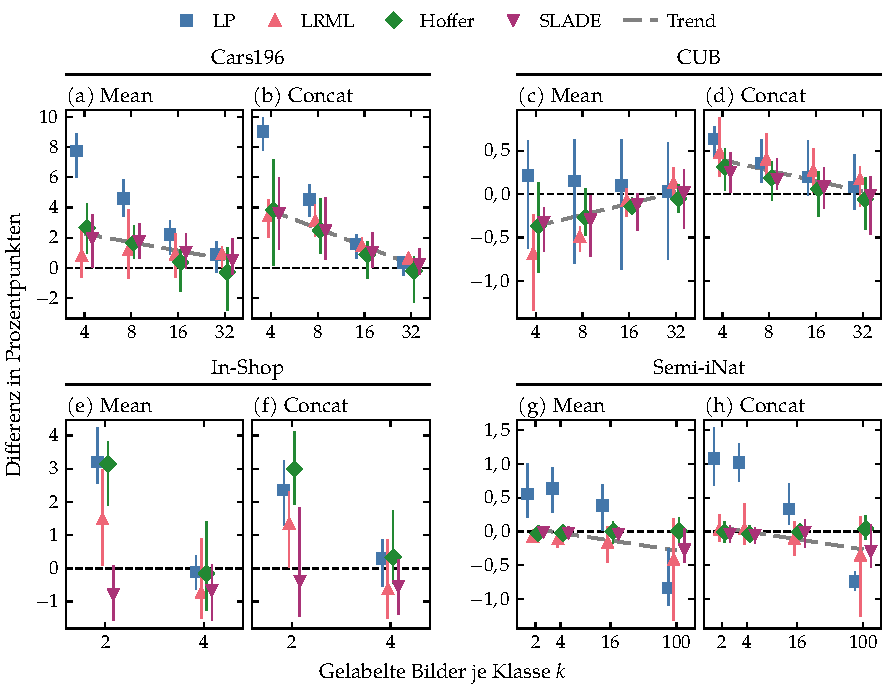
\includegraphics{neu/phase1_uebersicht}
  \caption[Gewinn der \acs{SSL}-Verfahren über das Label-Budget]{Gepaarter Gewinn der Test-\acs{MAP@R} der vier \acs{SSL}-Verfahren gegenüber der \UEBL, Mittel über die fünf Verlustfunktionen (Punkte) mit ihrer Spanne (senkrechte Striche). Grau gestrichelt: Trend über die vier Verfahren (lineare Anpassung an ihren Median je Budget), auf In-Shop mit nur zwei Budgets keiner. Je Datensatz links Mean, rechts Concat, die $y$-Achse ist je Datensatz anders skaliert.}
  \label{fig:e:uebersicht}
\end{figure}

\begin{figure}[tbp]
  \centering
  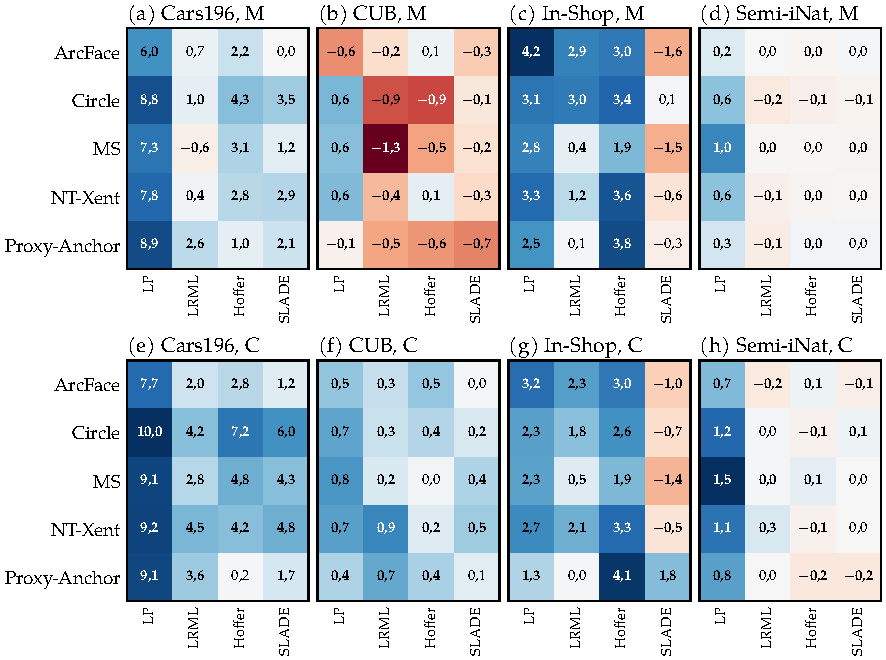
\includegraphics{neu/phase1_verluste}
  \caption[Gewinn je Verlustfunktion und Verfahren beim kleinsten Budget]{Gepaarter Gewinn der Test-\acs{MAP@R} je Verlustfunktion und Verfahren beim kleinsten Budget (Cars196 und \acs{CUB}: $k=4$, In-Shop und Semi-iNat-2021: $k=2$). (a) bis (d): Mean (M), (e) bis (h): Concat (C). Fett: Vorzeichen in allen fünf Seeds gleich. Farbskala je Datensatz symmetrisch um null.}
  \label{fig:e:verluste}
\end{figure}

\begin{table}[tbp]
\centering
\caption[Negative Vergleiche gegenüber der supervised Referenz]{Zahl der gepaarten Vergleiche (von 25), in denen ein \acs{SSL}-Verfahren eine niedrigere Test-MAP@R erreichte als die \UEBL, zu den Gewinnen in Tabelle \ref{tab:anhang:gewinne}. M: Mean, C: Concat.}
\label{tab:anhang:negativ}
\small
\begin{tabular}{@{}l *{8}{S[table-format=2.0]}@{}}
\toprule
\multicolumn{9}{@{}l}{\emph{Cars196}} \\
 & \multicolumn{2}{c}{$k=4$} & \multicolumn{2}{c}{$k=8$} & \multicolumn{2}{c}{$k=16$} & \multicolumn{2}{c}{$k=32$} \\
\cmidrule(lr){2-3}\cmidrule(lr){4-5}\cmidrule(lr){6-7}\cmidrule(lr){8-9}
 & {M} & {C} & {M} & {C} & {M} & {C} & {M} & {C} \\
LP & 0 & 0 & 0 & 0 & 0 & 0 & 5 & 5 \\
\acs{LRML} & 6 & 0 & 10 & 0 & 5 & 0 & 1 & 0 \\
Hoffer & 0 & 3 & 0 & 0 & 8 & 5 & 12 & 11 \\
SLADE & 2 & 0 & 0 & 0 & 3 & 2 & 11 & 13 \\
\midrule
\multicolumn{9}{@{}l}{\emph{\acs{CUB}}} \\
 & \multicolumn{2}{c}{$k=4$} & \multicolumn{2}{c}{$k=8$} & \multicolumn{2}{c}{$k=16$} & \multicolumn{2}{c}{$k=32$} \\
\cmidrule(lr){2-3}\cmidrule(lr){4-5}\cmidrule(lr){6-7}\cmidrule(lr){8-9}
 & {M} & {C} & {M} & {C} & {M} & {C} & {M} & {C} \\
LP & 10 & 0 & 9 & 2 & 7 & 5 & 10 & 12 \\
\acs{LRML} & 25 & 0 & 25 & 0 & 14 & 2 & 6 & 5 \\
Hoffer & 16 & 1 & 19 & 5 & 21 & 8 & 17 & 14 \\
SLADE & 25 & 4 & 22 & 3 & 15 & 7 & 10 & 10 \\
\midrule
\multicolumn{9}{@{}l}{\emph{In-Shop}} \\
 & \multicolumn{2}{c}{$k=2$} & \multicolumn{2}{c}{$k=4$} & {} & {} & {} & {} \\
\cmidrule(lr){2-3}\cmidrule(lr){4-5}
 & {M} & {C} & {M} & {C} & {} & {} & {} & {} \\
LP & 0 & 0 & 17 & 5 & {} & {} & {} & {} \\
\acs{LRML} & 3 & 3 & 19 & 20 & {} & {} & {} & {} \\
Hoffer & 0 & 0 & 14 & 12 & {} & {} & {} & {} \\
SLADE & 20 & 20 & 21 & 18 & {} & {} & {} & {} \\
\midrule
\multicolumn{9}{@{}l}{\emph{Semi-iNat-2021}} \\
 & \multicolumn{2}{c}{$k=2$} & \multicolumn{2}{c}{$k=4$} & \multicolumn{2}{c}{$k=16$} & \multicolumn{2}{c}{$k=100$} \\
\cmidrule(lr){2-3}\cmidrule(lr){4-5}\cmidrule(lr){6-7}\cmidrule(lr){8-9}
 & {M} & {C} & {M} & {C} & {M} & {C} & {M} & {C} \\
LP & 0 & 0 & 0 & 0 & 0 & 0 & 25 & 25 \\
\acs{LRML} & 23 & 8 & 23 & 14 & 19 & 17 & 20 & 17 \\
Hoffer & 19 & 15 & 17 & 18 & 10 & 16 & 14 & 11 \\
SLADE & 17 & 16 & 19 & 15 & 15 & 13 & 20 & 20 \\
\bottomrule
\end{tabular}
\end{table}

\begin{table}[tbp]
\centering
\caption[Gewinn der \acs{SSL}-Verfahren in \acs{MAP@R}, \acs{RP} und \acs{P@1}]{Gepaarter Gewinn der \acs{SSL}-Verfahren gegenüber der \UEBL in \acs{MAP@R}, \acs{RP} und \acs{P@1} in Prozentpunkten, gemittelt über die fünf Seeds und die fünf Verlustfunktionen. M: einzelne Fold-Modelle (Mean), C: Ensemble (Concat). In-Shop-Serie: Anteil vollständig gelabelter Klassen. Fett: größter gerundeter Gewinn je Zeile und Metrik, sofern er positiv ist.}
\label{tab:anhang:metriken}
\footnotesize\setlength{\tabcolsep}{2pt}
\begin{tabular}{@{}l r c@{\hspace{4pt}} *{12}{S[table-format=+1.1, retain-explicit-plus]}@{}}
\toprule
 & &  & \multicolumn{3}{c}{LP} & \multicolumn{3}{c}{\acs{LRML}} & \multicolumn{3}{c}{Hoffer} & \multicolumn{3}{c}{SLADE} \\
\cmidrule(lr){4-6}\cmidrule(lr){7-9}\cmidrule(lr){10-12}\cmidrule(l){13-15}
{Datensatz} & {Budget} &  & {\acs{MAP@R}} & {\acs{RP}} & {\acs{P@1}} & {\acs{MAP@R}} & {\acs{RP}} & {\acs{P@1}} & {\acs{MAP@R}} & {\acs{RP}} & {\acs{P@1}} & {\acs{MAP@R}} & {\acs{RP}} & {\acs{P@1}} \\
\midrule
Cars196 & 4 & M & \bfseries +7.8 & \bfseries +6.7 & \bfseries +3.4 & +0.8 & +0.5 & +0.1 & +2.7 & +2.1 & +1.5 & +2.0 & +1.3 & +1.1 \\
 &  & C & \bfseries +9.0 & \bfseries +7.4 & \bfseries +4.8 & +3.4 & +2.7 & +2.0 & +3.8 & +2.9 & +2.3 & +3.6 & +2.6 & +2.5 \\
 & 8 & M & \bfseries +4.6 & \bfseries +4.1 & \bfseries +1.2 & +1.2 & +1.1 & -0.4 & +1.7 & +1.3 & +0.4 & +1.7 & +1.4 & +0.7 \\
 &  & C & \bfseries +4.5 & \bfseries +3.7 & \bfseries +1.9 & +3.1 & +2.6 & +1.5 & +2.5 & +1.8 & +1.2 & +2.5 & +1.8 & +1.5 \\
 & 16 & M & \bfseries +2.2 & \bfseries +2.0 & \bfseries +0.1 & +0.9 & +1.0 & -0.6 & +0.4 & +0.3 & -0.7 & +1.1 & +0.8 & \bfseries +0.1 \\
 &  & C & \bfseries +1.6 & \bfseries +1.3 & +0.2 & +1.5 & +1.2 & +0.4 & +0.9 & +0.6 & +0.0 & +1.1 & +0.7 & \bfseries +0.5 \\
 & 32 & M & \bfseries +0.9 & +0.8 & +0.0 & \bfseries +0.9 & \bfseries +0.9 & +0.0 & -0.3 & -0.3 & -1.0 & +0.5 & +0.4 & \bfseries +0.2 \\
 &  & C & +0.4 & +0.3 & -0.2 & \bfseries +0.6 & \bfseries +0.6 & +0.0 & -0.2 & -0.3 & -0.6 & +0.2 & +0.1 & +0.0 \\
\addlinespace
\acs{CUB} & 4 & M & \bfseries +0.2 & \bfseries +0.2 & -0.2 & -0.7 & -0.6 & -0.6 & -0.4 & -0.3 & -0.4 & -0.3 & -0.3 & -0.3 \\
 &  & C & \bfseries +0.6 & \bfseries +0.6 & \bfseries +0.1 & +0.5 & +0.4 & +0.0 & +0.3 & +0.2 & +0.0 & +0.3 & +0.2 & \bfseries +0.1 \\
 & 8 & M & \bfseries +0.2 & \bfseries +0.2 & -0.2 & -0.5 & -0.4 & -0.5 & -0.3 & -0.2 & -0.3 & -0.3 & -0.3 & -0.2 \\
 &  & C & \bfseries +0.4 & \bfseries +0.3 & -0.1 & \bfseries +0.4 & \bfseries +0.3 & -0.1 & +0.2 & +0.2 & -0.1 & +0.2 & +0.1 & +0.0 \\
 & 16 & M & \bfseries +0.1 & \bfseries +0.1 & -0.1 & -0.1 & +0.0 & -0.1 & -0.1 & -0.1 & -0.1 & -0.1 & -0.1 & +0.0 \\
 &  & C & +0.2 & \bfseries +0.2 & +0.0 & \bfseries +0.3 & \bfseries +0.2 & \bfseries +0.1 & +0.1 & +0.0 & +0.0 & +0.1 & +0.1 & \bfseries +0.1 \\
 & 32 & M & +0.0 & \bfseries +0.1 & +0.0 & \bfseries +0.1 & \bfseries +0.1 & +0.0 & -0.1 & +0.0 & -0.1 & +0.0 & +0.0 & \bfseries +0.1 \\
 &  & C & +0.1 & +0.1 & +0.1 & \bfseries +0.2 & \bfseries +0.2 & +0.1 & -0.1 & -0.1 & +0.0 & +0.0 & +0.0 & \bfseries +0.2 \\
\addlinespace
In-Shop & 2 & M & \bfseries +3.2 & \bfseries +2.9 & \bfseries +2.5 & +1.5 & +1.3 & +1.3 & +3.1 & +2.8 & +1.9 & -0.8 & -0.7 & -0.8 \\
 &  & C & +2.4 & +2.1 & \bfseries +1.7 & +1.3 & +1.1 & +1.2 & \bfseries +3.0 & \bfseries +2.7 & \bfseries +1.7 & -0.4 & -0.3 & -0.4 \\
 & 4 & M & -0.1 & -0.1 & -0.7 & -0.7 & -0.7 & -0.4 & -0.2 & -0.2 & -1.1 & -0.7 & -0.6 & -0.7 \\
 &  & C & \bfseries +0.3 & \bfseries +0.3 & -0.5 & -0.6 & -0.6 & -0.3 & \bfseries +0.3 & \bfseries +0.3 & -0.8 & -0.5 & -0.5 & -0.6 \\
\addlinespace
In-Shop-Serie & 5\,\% & M & -1.6 & -1.5 & -1.9 & -0.1 & -0.2 & -0.3 & -0.1 & -0.1 & +0.0 & +0.0 & +0.0 & \bfseries +0.1 \\
 &  & C & -1.4 & -1.4 & -1.5 & \bfseries +1.3 & \bfseries +1.1 & \bfseries +1.0 & -0.2 & -0.1 & -0.1 & -0.1 & -0.2 & -0.1 \\
 & 10\,\% & M & -1.5 & -1.4 & -1.7 & \bfseries +0.3 & \bfseries +0.2 & +0.0 & -0.1 & -0.1 & -0.1 & -0.7 & -0.7 & -0.7 \\
 &  & C & -1.8 & -1.7 & -1.8 & \bfseries +0.9 & \bfseries +0.7 & \bfseries +0.6 & -0.2 & -0.2 & -0.3 & -1.0 & -1.0 & -0.9 \\
 & 25\,\% & M & -3.8 & -3.6 & -3.5 & -1.0 & -1.0 & -1.1 & -0.1 & -0.1 & +0.0 & -2.1 & -2.0 & -1.8 \\
 &  & C & -3.3 & -3.1 & -2.9 & -1.0 & -1.0 & -0.9 & -0.2 & -0.2 & -0.1 & -2.4 & -2.3 & -2.0 \\
 & 50\,\% & M & -4.8 & -4.5 & -4.2 & -2.2 & -2.1 & -2.1 & +0.0 & +0.0 & +0.0 & -2.1 & -2.0 & -1.7 \\
 &  & C & -3.9 & -3.6 & -3.2 & -2.0 & -1.9 & -1.8 & -0.1 & +0.0 & -0.1 & -1.9 & -1.8 & -1.6 \\
\addlinespace
Semi-iNat & 2 & M & \bfseries +0.6 & \bfseries +0.6 & \bfseries +0.1 & -0.1 & -0.1 & +0.0 & +0.0 & +0.0 & +0.0 & +0.0 & +0.0 & +0.0 \\
 &  & C & \bfseries +1.1 & \bfseries +1.1 & \bfseries +0.3 & +0.0 & +0.0 & +0.0 & +0.0 & +0.0 & +0.0 & +0.0 & +0.0 & +0.0 \\
 & 4 & M & \bfseries +0.6 & \bfseries +0.7 & \bfseries +0.1 & -0.1 & -0.1 & -0.1 & +0.0 & +0.0 & +0.0 & +0.0 & +0.0 & +0.0 \\
 &  & C & \bfseries +1.0 & \bfseries +1.0 & \bfseries +0.3 & +0.0 & +0.0 & +0.0 & +0.0 & +0.0 & +0.0 & -0.1 & +0.0 & +0.0 \\
 & 16 & M & \bfseries +0.4 & \bfseries +0.4 & \bfseries +0.1 & -0.2 & -0.2 & -0.1 & +0.0 & +0.0 & +0.0 & +0.0 & +0.0 & +0.0 \\
 &  & C & \bfseries +0.3 & \bfseries +0.3 & \bfseries +0.1 & -0.1 & -0.1 & -0.1 & +0.0 & +0.0 & +0.0 & +0.0 & +0.0 & +0.0 \\
 & 100 & M & -0.8 & -0.9 & -0.4 & -0.4 & -0.4 & -0.2 & +0.0 & +0.0 & +0.0 & -0.3 & -0.2 & -0.1 \\
 &  & C & -0.7 & -0.8 & -0.3 & -0.4 & -0.4 & -0.2 & +0.0 & +0.0 & +0.0 & -0.3 & -0.3 & -0.1 \\
\bottomrule
\end{tabular}
\end{table}

\clearpage
\begin{table}[htbp]
\centering
\caption[Übernommene Konfigurationen Cars196]{Für die Wiederholungen übernommene HPO-Konfigurationen (Optimierung bei $k=16$, Seed~7). Versuch: Nummer innerhalb der Suche, $B$: supervised bzw. gemischte Batchgröße, Warm-up in Epochen. Wiederholungen mit höchstens \num{1000} Epochen und einer Patience von 20 Epochen. Übrige Loss-, Miner- und SSL-Parameter im digitalen Anhang.}
\label{tab:cars:hpo}
\begin{tabular}{@{}llrrrr@{}}
\toprule
Verlust & Verf. & Versuch & Lernrate & $B$ & Warm-up \\
\midrule
ArcFace & \UEBL & 56 & \num{1.052e-05} & 32 & 0 \\
ArcFace & LP & 41 & \num{8.308e-01} & 32 & 10 \\
ArcFace & LRML & 66 & \num{1.782e-04} & 128 & 30 \\
ArcFace & Hoffer & 73 & \num{2.428e-05} & 32 & 15 \\
ArcFace & SLADE & 65 & \num{1.468e-04} & 256 & 15 \\
\addlinespace[3pt]
Circle & \UEBL & 71 & \num{3.717e-05} & 32 & 0 \\
Circle & LP & 74 & \num{1.304e-05} & 32 & 20 \\
Circle & LRML & 56 & \num{3.775e-05} & 64 & 20 \\
Circle & Hoffer & 37 & \num{8.366e-05} & 64 & 10 \\
Circle & SLADE & 67 & \num{1.188e-04} & 64 & 20 \\
\addlinespace[3pt]
Multi-Similarity & \UEBL & 65 & \num{1.002e-05} & 32 & 0 \\
Multi-Similarity & LP & 76 & \num{8.125e-05} & 64 & 5 \\
Multi-Similarity & LRML & 70 & \num{1.258e-04} & 64 & 30 \\
Multi-Similarity & Hoffer & 58 & \num{2.185e-05} & 64 & 25 \\
Multi-Similarity & SLADE & 55 & \num{7.300e-05} & 64 & 15 \\
\addlinespace[3pt]
NT-Xent & \UEBL & 61 & \num{1.688e-05} & 128 & 0 \\
NT-Xent & LP & 74 & \num{2.213e-05} & 128 & 15 \\
NT-Xent & LRML & 28 & \num{3.676e-04} & 256 & 10 \\
NT-Xent & Hoffer & 0 & \num{2.114e-04} & 128 & 5 \\
NT-Xent & SLADE & 67 & \num{1.654e-04} & 256 & 5 \\
\addlinespace[3pt]
Proxy-Anchor & \UEBL & 79 & \num{8.236e-04} & 32 & 0 \\
Proxy-Anchor & LP & 39 & \num{1.544e-05} & 64 & 10 \\
Proxy-Anchor & LRML & 54 & \num{2.539e-05} & 64 & 30 \\
Proxy-Anchor & Hoffer & 55 & \num{1.070e-04} & 256 & 5 \\
Proxy-Anchor & SLADE & 66 & \num{7.725e-05} & 32 & 0 \\
\bottomrule
\end{tabular}
\end{table}

\begin{table}[htbp]
\centering
\caption[Übernommene Konfigurationen CUB]{Für die Wiederholungen übernommene HPO-Konfigurationen (Optimierung bei $k=16$, Seed 7). Versuch: Nummer innerhalb der Suche, $B$: supervised bzw. gemischte Batchgröße, Warm-up in Epochen. Wiederholungen mit höchstens \num{1000} Epochen und einer Patience von 40 Epochen. Übrige Loss-, Miner- und SSL-Parameter im GitHub-Repository.}
\label{tab:cub:hpo}
\begin{tabular}{@{}llrrrr@{}}
\toprule
Verlust & Verf. & Versuch & Lernrate & $B$ & Warm-up \\
\midrule
ArcFace & \UEBL & 63 & \num{7.573e-05} & 32 & 0 \\
ArcFace & LP & 65 & \num{3.147e+00} & 256 & 8 \\
ArcFace & LRML & 66 & \num{7.448e-05} & 64 & 12 \\
ArcFace & Hoffer & 79 & \num{1.914e-04} & 256 & 6 \\
ArcFace & SLADE & 46 & \num{7.016e-05} & 64 & 10 \\
\addlinespace[3pt]
Circle & \UEBL & 77 & \num{5.327e-05} & 128 & 0 \\
Circle & LP & 14 & \num{1.784e-05} & 128 & 12 \\
Circle & LRML & 53 & \num{3.461e-05} & 128 & 12 \\
Circle & Hoffer & 77 & \num{7.473e-05} & 256 & 6 \\
Circle & SLADE & 50 & \num{5.005e-05} & 128 & 2 \\
\addlinespace[3pt]
Multi-Similarity & \UEBL & 50 & \num{2.283e-05} & 64 & 0 \\
Multi-Similarity & LP & 63 & \num{1.650e-05} & 128 & 0 \\
Multi-Similarity & LRML & 78 & \num{7.680e-05} & 256 & 8 \\
Multi-Similarity & Hoffer & 70 & \num{4.738e-05} & 128 & 10 \\
Multi-Similarity & SLADE & 73 & \num{4.141e-05} & 128 & 8 \\
\addlinespace[3pt]
NT-Xent & \UEBL & 72 & \num{5.022e-05} & 256 & 0 \\
NT-Xent & LP & 47 & \num{2.186e-05} & 256 & 4 \\
NT-Xent & LRML & 49 & \num{5.863e-05} & 256 & 12 \\
NT-Xent & Hoffer & 45 & \num{5.468e-05} & 256 & 0 \\
NT-Xent & SLADE & 70 & \num{4.260e-05} & 256 & 10 \\
\addlinespace[3pt]
Proxy-Anchor & \UEBL & 61 & \num{7.044e-05} & 128 & 0 \\
Proxy-Anchor & LP & 49 & \num{1.834e-04} & 32 & 2 \\
Proxy-Anchor & LRML & 40 & \num{3.401e-04} & 128 & 6 \\
Proxy-Anchor & Hoffer & 74 & \num{2.856e-04} & 128 & 8 \\
Proxy-Anchor & SLADE & 57 & \num{9.107e-05} & 256 & 10 \\
\bottomrule
\end{tabular}
\end{table}

\begin{table}[htbp]
\centering
\caption[Übernommene Konfigurationen In-Shop]{Für die Wiederholungen übernommene HPO-Konfigurationen (Optimierung bei $k=2$, Seed~7). Versuch: Nummer innerhalb der Suche, $B$: supervised bzw. gemischte Batchgröße, Warm-up in Epochen. Wiederholungen mit höchstens \num{1000} Epochen und einer Patience von 20 Epochen. Übrige Loss-, Miner- und SSL-Parameter im digitalen Anhang.}
\label{tab:inshop:hpo}
\begin{tabular}{@{}llrrrr@{}}
\toprule
Verlust & Verf. & Versuch & Lernrate & $B$ & Warm-up \\
\midrule
ArcFace & \UEBL & 42 & \num{6.684e-01} & 512 & 0 \\
ArcFace & LP & 73 & \num{5.654e-02} & 64 & 15 \\
ArcFace & LRML & 63 & \num{2.025e-04} & 512 & 30 \\
ArcFace & Hoffer & 50 & \num{1.599e-01} & 256 & 30 \\
ArcFace & SLADE & 48 & \num{1.137e-04} & 256 & 0 \\
\addlinespace[3pt]
Circle & \UEBL & 45 & \num{1.153e-05} & 128 & 0 \\
Circle & LP & 75 & \num{2.150e-05} & 256 & 10 \\
Circle & LRML & 44 & \num{2.009e-05} & 128 & 15 \\
Circle & Hoffer & 65 & \num{5.250e-05} & 128 & 0 \\
Circle & SLADE & 61 & \num{1.324e-05} & 256 & 20 \\
\addlinespace[3pt]
Multi-Similarity & \UEBL & 77 & \num{1.315e-05} & 256 & 0 \\
Multi-Similarity & LP & 78 & \num{5.384e-05} & 256 & 25 \\
Multi-Similarity & LRML & 58 & \num{3.606e-05} & 128 & 20 \\
Multi-Similarity & Hoffer & 75 & \num{4.516e-05} & 64 & 15 \\
Multi-Similarity & SLADE & 44 & \num{3.350e-04} & 512 & 15 \\
\addlinespace[3pt]
NT-Xent & \UEBL & 69 & \num{1.949e-05} & 512 & 0 \\
NT-Xent & LP & 58 & \num{4.129e-05} & 512 & 20 \\
NT-Xent & LRML & 65 & \num{7.505e-05} & 256 & 20 \\
NT-Xent & Hoffer & 45 & \num{2.841e-05} & 64 & 20 \\
NT-Xent & SLADE & 62 & \num{6.076e-05} & 512 & 15 \\
\addlinespace[3pt]
Proxy-Anchor & \UEBL & 52 & \num{1.905e-05} & 128 & 0 \\
Proxy-Anchor & LP & 41 & \num{5.646e-05} & 128 & 25 \\
Proxy-Anchor & LRML & 74 & \num{5.762e-02} & 512 & 10 \\
Proxy-Anchor & Hoffer & 75 & \num{1.325e-02} & 256 & 0 \\
Proxy-Anchor & SLADE & 46 & \num{4.633e-04} & 128 & 5 \\
\bottomrule
\end{tabular}
\end{table}

\begin{table}[htbp]
\centering
\caption[Übernommene Konfigurationen In-Shop mit gelabelten Klassen]{Für die Wiederholungen übernommene HPO-Konfigurationen (Optimierung bei 10\,\% vollständig gelabelten Klassen, Seed 7). Versuch: Nummer innerhalb der Suche, $B$: supervised bzw. gemischte Batchgröße, Warm-up in Epochen. Wiederholungen mit höchstens \num{1000} Epochen und einer Patience von 20 Epochen. Verzögerte Patience (Abschnitt \ref{sec:training}) für die \UEBL mit Proxy-Anchor bei 10 bis 50\,\% gelabelter Klassen. Übrige Loss-, Miner- und SSL-Parameter im GitHub-Repository.}
\label{tab:inshop10:hpo}
\small
\begin{tabular}{@{}llrrrr@{}}
\toprule
Verlust & Verf. & Versuch & Lernrate & $B$ & Warm-up \\
\midrule
ArcFace & \UEBL & 68 & \num{2.572e-04} & 256 & 0 \\
ArcFace & LP & 24 & \num{1.459e-03} & 64 & 15 \\
ArcFace & LRML & 77 & \num{2.666e-03} & 512 & 30 \\
ArcFace & Hoffer & 74 & \num{2.348e-05} & 256 & 5 \\
ArcFace & SLADE & 57 & \num{8.623e-05} & 256 & 20 \\
\addlinespace[3pt]
Circle & \UEBL & 61 & \num{1.667e-05} & 128 & 0 \\
Circle & LP & 79 & \num{6.327e-05} & 128 & 25 \\
Circle & LRML & 65 & \num{4.945e-05} & 256 & 20 \\
Circle & Hoffer & 53 & \num{2.197e-05} & 128 & 0 \\
Circle & SLADE & 71 & \num{1.560e-05} & 256 & 15 \\
\addlinespace[3pt]
Multi-Similarity & \UEBL & 73 & \num{1.052e-05} & 256 & 0 \\
Multi-Similarity & LP & 78 & \num{1.648e-05} & 256 & 5 \\
Multi-Similarity & LRML & 62 & \num{1.672e-04} & 512 & 20 \\
Multi-Similarity & Hoffer & 73 & \num{3.291e-05} & 512 & 5 \\
Multi-Similarity & SLADE & 74 & \num{3.039e-05} & 512 & 10 \\
\addlinespace[3pt]
NT-Xent & \UEBL & 74 & \num{1.028e-05} & 512 & 0 \\
NT-Xent & LP & 53 & \num{9.070e-05} & 512 & 30 \\
NT-Xent & LRML & 65 & \num{1.112e-04} & 512 & 5 \\
NT-Xent & Hoffer & 44 & \num{2.298e-05} & 512 & 25 \\
NT-Xent & SLADE & 64 & \num{1.230e-04} & 256 & 25 \\
\addlinespace[3pt]
Proxy-Anchor & \UEBL & 69 & \num{7.223e+00} & 512 & 0 \\
Proxy-Anchor & LP & 68 & \num{1.578e-03} & 256 & 25 \\
Proxy-Anchor & LRML & 40 & \num{3.542e-04} & 64 & 25 \\
Proxy-Anchor & Hoffer & 62 & \num{2.656e-05} & 128 & 0 \\
Proxy-Anchor & SLADE & 68 & \num{5.491e-05} & 128 & 10 \\
\bottomrule
\end{tabular}
\end{table}

\begin{table}[htbp]
\centering
\caption[Übernommene Konfigurationen Semi-iNat-2021]{Für die Wiederholungen übernommene HPO-Konfigurationen (Optimierung bei $k=16$, Seed 7). Versuch: Nummer innerhalb der Suche, $B$: supervised bzw. gemischte Batchgröße, Warm-up in Epochen, Ep./Patience: Epochenlimit und Early-Stopping-Patience der Wiederholungen. Übrige Loss-, Miner- und SSL-Parameter im digitalen Anhang.}
\label{tab:semiinat:hpo}
\begin{tabular}{@{}llrrrrr@{}}
\toprule
Verlust & Verf. & Versuch & Lernrate & $B$ & Warm-up & Ep./Patience \\
\midrule
ArcFace & \UEBL & 71 & \num{7.811e-06} & 512 & 0 & 1000/10 \\
ArcFace & LP & 49 & \num{1.255e-05} & 128 & 2 & 1000/10 \\
ArcFace & LRML & 53 & \num{1.072e-05} & 512 & 1 & 1000/10 \\
ArcFace & Hoffer & 55 & \num{2.133e-05} & 256 & 0 & 1000/10 \\
ArcFace & SLADE & 57 & \num{6.447e-06} & 512 & 2 & 1000/10 \\
\addlinespace[3pt]
Circle & \UEBL & 61 & \num{5.660e-06} & 128 & 0 & 1000/10 \\
Circle & LP & 75 & \num{5.812e-06} & 128 & 0 & 1000/10 \\
Circle & LRML & 47 & \num{1.110e-05} & 256 & 0 & 1000/10 \\
Circle & Hoffer & 23 & \num{2.042e-05} & 256 & 2 & 1000/10 \\
Circle & SLADE & 77 & \num{2.088e-05} & 256 & 2 & 1000/10 \\
\addlinespace[3pt]
Multi-Similarity & \UEBL & 77 & \num{2.246e-05} & 128 & 0 & 1000/10 \\
Multi-Similarity & LP & 53 & \num{6.428e-06} & 256 & 2 & 1000/10 \\
Multi-Similarity & LRML & 51 & \num{1.418e-05} & 512 & 0 & 1000/10 \\
Multi-Similarity & Hoffer & 74 & \num{5.119e-05} & 256 & 0 & 1000/10 \\
Multi-Similarity & SLADE & 80 & \num{1.847e-05} & 512 & 0 & 1000/10 \\
\addlinespace[3pt]
NT-Xent & \UEBL & 71 & \num{1.989e-05} & 512 & 0 & 1000/10 \\
NT-Xent & LP & 55 & \num{1.861e-05} & 512 & 4 & 1000/10 \\
NT-Xent & LRML & 78 & \num{9.365e-05} & 512 & 2 & 1000/10 \\
NT-Xent & Hoffer & 76 & \num{1.576e-05} & 512 & 0 & 1000/10 \\
NT-Xent & SLADE & 79 & \num{1.382e-05} & 512 & 1 & 1000/10 \\
\addlinespace[3pt]
Proxy-Anchor & \UEBL & 76 & \num{5.343e-06} & 256 & 0 & 1000/10 \\
Proxy-Anchor & LP & 48 & \num{2.811e-05} & 256 & 6 & 1000/10 \\
Proxy-Anchor & LRML & 57 & \num{2.349e-05} & 512 & 0 & 1000/10 \\
Proxy-Anchor & Hoffer & 75 & \num{1.842e-05} & 512 & 1 & 1000/10 \\
Proxy-Anchor & SLADE & 64 & \num{6.179e-06} & 256 & 1 & 1000/10 \\
\bottomrule
\end{tabular}
\end{table}

\begin{table}[tbp]
\centering\small\setlength{\tabcolsep}{4pt}
\caption[Rechenzeit der Verfahren]{Rechenzeit der Verfahren beim Budget der Hyperparametersuche (Abschnitt \ref{sec:m:aufwand}), Median über die Verlustfunktionen. Schritt und Epoche nach dem Warm-up, Neuberechnung je Epoche über alle Batchgrößen $B$. Epochen und Fold: trainierte Epochen der Phase-1-Folds und daraus berechnete Dauer, Median über 100 Folds. Auf Semi-iNat-2021 fehlt \acs{NT-Xent} bei Hoffer für $B=128$ und bei \acs{SLADE} für $B=32$ und 64.}
\label{tab:anhang:aufwand}
\begin{tabular}{@{}l *{5}{c}@{}}
\toprule
 & \UEBL & \acs{LP} & \acs{LRML} & Hoffer & \acs{SLADE} \\
\midrule
\multicolumn{6}{@{}l}{\textbf{Cars196 ($k=16$)}} \\*
\quad Schritt in ms bei $B=128$ & \num{2.8} & \num{4.2} & \num{7.5} & \num{9.4} & \num{16.6} \\
\quad Epoche in s bei $B=32$ & \num{0.50} & \num{1.07} & \num{1.47} & \num{1.84} & \num{3.46} \\
\quad \phantom{Epoche in s bei }$B=64$ & \num{0.30} & \num{0.84} & \num{1.02} & \num{0.87} & \num{2.01} \\
\quad \phantom{Epoche in s bei }$B=128$ & \num{0.22} & \num{0.65} & \num{0.81} & \num{0.56} & \num{1.00} \\
\quad \phantom{Epoche in s bei }$B=256$ & \num{0.16} & \num{0.60} & \num{0.69} & \num{0.33} & \num{0.65} \\
\quad Neuberechnung in s & -- & \num{0.39} & \num{0.39} & \num{0.00} & \num{0.09} \\
\quad Epochen & \num{100} & \num{168} & \num{69} & \num{65} & \num{52} \\
\quad Fold in min & \num{0.4} & \num{2.3} & \num{0.8} & \num{0.8} & \num{1.2} \\
\midrule
\multicolumn{6}{@{}l}{\textbf{Semi-iNat-2021 ($k=16$)}} \\*
\quad Schritt in ms bei $B=128$ & \num{1.9} & \num{2.2} & \num{4.1} & \num{6.8} & \num{11.7} \\
\quad Epoche in s bei $B=32$ & \num{1.85} & \num{3.35} & \num{6.07} & \num{8.84} & \num{16.57} \\
\quad \phantom{Epoche in s bei }$B=64$ & \num{1.16} & \num{2.67} & \num{3.91} & \num{4.73} & \num{8.94} \\
\quad \phantom{Epoche in s bei }$B=128$ & \num{0.85} & \num{2.36} & \num{2.81} & \num{2.60} & \num{5.01} \\
\quad \phantom{Epoche in s bei }$B=256$ & \num{0.67} & \num{2.02} & \num{2.31} & \num{1.58} & \num{3.30} \\
\quad \phantom{Epoche in s bei }$B=512$ & \num{0.54} & \num{1.92} & \num{2.01} & \num{0.99} & \num{2.30} \\
\quad Neuberechnung in s & -- & \num{1.26} & \num{1.21} & \num{0.00} & \num{0.77} \\
\quad Epochen & \num{52} & \num{63} & \num{41} & \num{31} & \num{62} \\
\quad Fold in min & \num{0.7} & \num{2.4} & \num{1.5} & \num{0.7} & \num{2.6} \\
\midrule
\multicolumn{6}{@{}l}{\textbf{In-Shop ($k=2$)}} \\*
\quad Schritt in ms bei $B=128$ & \num{3.3} & \num{4.7} & \num{6.3} & \num{24.8} & \num{16.2} \\
\quad Epoche in s bei $B=32$ & \num{1.90} & \num{4.00} & \num{3.50} & \num{14.25} & \num{10.24} \\
\quad \phantom{Epoche in s bei }$B=64$ & \num{1.02} & \num{2.86} & \num{2.52} & \num{7.47} & \num{5.25} \\
\quad \phantom{Epoche in s bei }$B=128$ & \num{0.59} & \num{2.59} & \num{1.55} & \num{3.88} & \num{2.72} \\
\quad \phantom{Epoche in s bei }$B=256$ & \num{0.43} & \num{2.22} & \num{1.19} & \num{2.09} & \num{1.66} \\
\quad \phantom{Epoche in s bei }$B=512$ & \num{0.34} & \num{2.11} & \num{1.00} & \num{1.17} & \num{1.02} \\
\quad Neuberechnung in s & -- & \num{1.69} & \num{0.48} & \num{0.00} & \num{0.12} \\
\quad Epochen & \num{258} & \num{254} & \num{176} & \num{155} & \num{178} \\
\quad Fold in min & \num{2.0} & \num{8.9} & \num{3.4} & \num{10.4} & \num{6.8} \\
\midrule
\multicolumn{6}{@{}l}{\textbf{In-Shop-Serie mit gelabelten Klassen (\qty{10}{\percent})}} \\*
\quad Schritt in ms bei $B=128$ & \num{3.0} & \num{2.1} & -- & \num{10.0} & \num{16.4} \\
\quad Epoche in s bei $B=32$ & \num{1.91} & \num{2.62} & -- & \num{6.27} & \num{10.11} \\
\quad \phantom{Epoche in s bei }$B=64$ & \num{0.98} & \num{2.36} & -- & \num{3.05} & \num{5.41} \\
\quad \phantom{Epoche in s bei }$B=128$ & \num{0.54} & \num{2.14} & -- & \num{1.62} & \num{2.79} \\
\quad \phantom{Epoche in s bei }$B=256$ & \num{0.38} & \num{2.06} & -- & \num{0.89} & \num{1.57} \\
\quad \phantom{Epoche in s bei }$B=512$ & \num{0.27} & \num{1.85} & -- & \num{0.55} & \num{1.11} \\
\quad Neuberechnung in s & -- & \num{1.59} & -- & \num{0.00} & \num{0.15} \\
\quad Epochen & \num{184} & \num{47} & \num{73} & \num{144} & \num{128} \\
\quad Fold in min & \num{1.3} & \num{1.0} & -- & \num{3.8} & \num{3.3} \\
\bottomrule
\end{tabular}
\end{table}


\chapter{Alle Varianten der Phase 2}
\label{chap:anhang:phase2}

Dieser Anhang ergänzt Abschnitt \ref{sec:e:phase2}. Die Tabellen \ref{tab:anhang:phase2} und \ref{tab:anhang:phase2:inshop} enthalten die Test-\ac{MAP@R} aller Varianten auf Cars196 und In-Shop mit allen fünf Verlustfunktionen, die Tabellen \ref{tab:anhang:phase2:concat} und \ref{tab:anhang:phase2:inshop:concat} dieselben Varianten als Concat-\ac{MAP@R}, also für das Ensemble der Fold-Modelle. Tabelle \ref{tab:anhang:phase2:slade} enthält die Sweeps von \ac{SLADE} (Abschnitt \ref{sec:e:sweeps}), Tabelle \ref{tab:anhang:phase2:k8} alle Varianten auf Cars196 mit $k=8$ (Abschnitt \ref{sec:e:phase2:k8}). Mit der verzögerten Patience (Abschnitt \ref{sec:training}) wichen die regulären Konfigurationen dort höchstens \num{0.22} Prozentpunkte von den Phase-1-Läufen mit Seed 2 bei $k=8$ ab. Die Tabellen \ref{tab:anhang:extern:cars}, \ref{tab:anhang:extern:inshop} und \ref{tab:anhang:extern:sweeps} enthalten die Einzelwerte des Versuchs mit externen ungelabelten Bildern (Abschnitt \ref{sec:e:extern}), der wie Phase 2 mit Seed 2 lief. Abbildung \ref{fig:e:lppseudolabels} zeigt die Pseudo-Labels von \ac{LP} über alle Budgets (Abschnitt \ref{sec:e:pseudolabels}).

\clearpage
\begingroup\small\setstretch{1}
\begin{longtable}{@{}>{\raggedright\arraybackslash\hspace{0pt}}p{4.0cm}>{\raggedright\arraybackslash\hspace{0pt}}p{5.5cm}>{\raggedright\arraybackslash\hspace{0pt}}p{4.4cm}@{}}
  \caption[Eingriffe der Phase 2 und vorab festgelegte Erwartungen]{Eingriffe der Phase 2 und die vor den Läufen festgelegten Erwartungen. Oracle-Varianten dienen nur der Diagnose. Sie verwenden die verdeckten Labels der ungelabelten Bilder, die sonst nie in das Training oder die Auswahl eingehen.}\label{tab:phase2:eingriffe}\\
    \toprule
    Eingriff & Umsetzung & Erwartung \\
    \midrule
    \endfirsthead
    \multicolumn{3}{@{}l}{\small Tabelle \thetable{} (Fortsetzung)}\\
    \toprule
    Eingriff & Umsetzung & Erwartung \\
    \midrule
    \endhead
    \bottomrule
    \endlastfoot
    ohne ungelabelte Bilder & mit der \acs{SSL}-Konfiguration erhält der \acs{SSL}-Mechanismus statt der ungelabelten die gelabelten Bilder, ohne deren Labels und mit derselben Zahl von Updates je Epoche. Mit den Hyperparametern der \UEBL ist der Lauf ohne ungelabelte Bilder die \UEBL selbst, also auch ohne \acs{SSL}-Mechanismus. Bei \acs{LP} tritt die Kontrolle mit abgeschaltetem \acs{SSL}-Mechanismus an ihre Stelle & \acs{MAP@R} sinkt mit beiden Hyperparametersätzen \\
    \addlinespace
    \acs{SSL}-Mechanismus abgeschaltet & \acs{SSL}-Konfiguration ohne \acs{SSL}-Term, bei \acs{LP} ohne Pseudo-Labels & Niveau der \UEBL \\
    \addlinespace
    Oracle-Pseudo-Labels (\acs{LP}) & genau die von \acs{LP} übernommenen Bilder erhalten ihr wahres Label, von dem ein Anteil von 0, 10, 20, 40 oder \SI{60}{\percent} zufällig durch ein falsches ersetzt wird & \acs{MAP@R} fällt mit dem Anteil, reguläres \acs{LP} liegt auf dieser Kurve \\
    \addlinespace
    Pseudo-Labels bzw.\ Graph eingefroren & nach dem Warm-up einmal berechnet und nicht mehr erneuert & ungerichtet \\
    \addlinespace
    Graph umverdrahtet (\acs{LP}, \acs{LRML}) & Kanten werden unter Erhalt der Knotengrade zufällig getauscht \cite{maslov_specificity_2002} & Gewinn verschwindet \\
    \addlinespace
    Oracle-Kanten entfernt, Kontrolle: zufällige Kanten entfernt & mit den verdeckten Labels werden alle Kanten zwischen verschiedenen Klassen entfernt, als Kontrolle dieselbe Zahl zufälliger Kanten & Oracle besser als regulär, Kontrolle nicht \\
    \addlinespace
    ohne Warm-up & \acs{SSL}-Konfiguration ohne Warm-up & ungerichtet \\
    \addlinespace
    Sweeps & je ein Hyperparameter wird variiert (bei \acs{LP} Nachbarzahl, Konfidenzschwelle und Warm-up, bei \acs{LRML} Nachbarzahl und $\eta$, bei Hoffer $\gamma_{\mathrm{H}}$ und $\eta$, bei \acs{SLADE} Clusterverhältnis, Intervall der Teacher-Aktualisierung, $\eta$, Basis-Zielverhältnis, ungelabelte Batchgröße und Marge von $\mathcal{L}_{\mathrm{SD}}$) & \acs{LP}: umgekehrt U-förmig in der Nachbarzahl, Abdeckung wichtiger als Genauigkeit, langes Warm-up vorteilhaft. \acs{LRML}: Optimum, solange die Kanten rein sind, Abfall bei zu großem $\eta$. Hoffer: zu kleine $\gamma_{\mathrm{H}}$ schaden (nach den Läufen korrigiert, Abschnitt \ref{sec:m:phase2}), Abfall bei zu großem $\eta$. \acs{SLADE}: ohne gerichtete Erwartung \\
    \addlinespace
    Vielfalt der Fold-Modelle & Anteil der falschen Nachbarn eines Fold-Modells unter den ersten $R_q$ Treffern, die ein anderes Fold-Modell ebenfalls hat & \acs{LRML}: geringerer Anteil als bei der \UEBL, daher größerer Abstand zwischen Concat und Mean \\
\end{longtable}
\endgroup

\begin{table}[tbp]
\centering\small\setstretch{1}\setlength{\tabcolsep}{4pt}
\caption[Vorab festgelegte Erwartungen der Phase 2 und Ergebnis]{Vorab festgelegte Erwartungen der Phase 2 (Tabelle \ref{tab:phase2:eingriffe} und Abschnitt \ref{sec:m:geometrie}) und ihr Ergebnis. Cars196 bei $k=16$ und In-Shop bei $k=2$ mit einem Seed, die Vielfalt der Fold-Modelle auf Cars196 bei $k=4$ mit fünf Seeds und die Geometrie über alle Budgets.}
\label{tab:a:erwartungen}
\begin{tabular}{@{}>{\raggedright\arraybackslash}p{3.0cm}>{\raggedright\arraybackslash}p{4.0cm}>{\raggedright\arraybackslash}p{5.0cm}l@{}}
\toprule
Eingriff & Erwartung & Ergebnis & Abschnitt \\
\midrule
Ohne ungelabelte Bilder & \acs{MAP@R} sinkt mit beiden Hyperparametersätzen & teilweise: mit den \acs{SSL}-Hyperparametern sank sie in 32 von 40 Kombinationen. Mit den Hyperparametern der \UEBL lag die Variante mit \acs{SSL}-Mechanismus und ungelabelten Bildern in 18 über und in 14 unter der \UEBL & \ref{sec:e:2x2} \\
\acs{SSL}-Mechanismus abgeschaltet & Niveau der \UEBL & teilweise: nur in 14 von 40 Kombinationen, in 25 darunter, in einer darüber & \ref{sec:e:2x2} \\
Oracle-Pseudo-Labels (\acs{LP}) & \acs{MAP@R} fällt mit dem Anteil, reguläres \acs{LP} liegt auf der Kurve & teilweise: auf der Kurve nur mit ArcFace und \acs{NT-Xent} auf Cars196, sonst darüber & \ref{sec:e:pseudolabels} \\
Pseudo-Labels bzw.\ Graph eingefroren & ungerichtet & \acs{LP} verlor auf In-Shop mit jeder Verlustfunktion & \ref{sec:e:nachbarschaft} \\
Graph umverdrahtet & Gewinn verschwindet & bestätigt, in allen 20 Kombinationen & \ref{sec:e:nachbarschaft} \\
Oracle-Kanten entfernt, Kontrolle: zufällige Kanten entfernt & Oracle besser als regulär, Kontrolle nicht & teilweise: Oracle nur in 12 von 20 besser, \acs{LP} mit ArcFace auf In-Shop schlechter. Kontrolle in keiner besser & \ref{sec:e:nachbarschaft} \\
\acs{LP}: Nachbarzahl & umgekehrt U-förmig & nicht bestätigt & \ref{sec:e:sweeps} \\
\acs{LP}: Konfidenzschwelle & Abdeckung wichtiger als Genauigkeit & teilweise: eine hohe Schwelle schadete auf Cars196 mit ArcFace, Circle und \acs{MS}, auf In-Shop mit Circle, half dort aber mit Proxy-Anchor. Mit ArcFace schadete auf In-Shop jede andere Schwelle & \ref{sec:e:sweeps} \\
\acs{LP}: Warm-up & langes Warm-up vorteilhaft & nicht bestätigt & \ref{sec:e:sweeps} \\
\acs{LRML}: Nachbarzahl und $\eta$ & Optimum, solange die Kanten rein sind, Abfall bei zu großem $\eta$ & teilweise: zu großes $\eta$ schadete in 9 von 10 Kombinationen. Die Reinheit stammt nur aus Geometrieläufen mit anderer Konfiguration, die beste Nachbarzahl war auf In-Shop viel kleiner als auf Cars196 & \ref{sec:e:sweeps} \\
Hoffer: $\gamma_{\mathrm{H}}$ & zu kleine $\gamma_{\mathrm{H}}$ schaden & bestätigt. Erwartung nach den Läufen korrigiert, davor: zu große $\gamma_{\mathrm{H}}$ schaden & \ref{sec:e:sweeps} \\
Hoffer: $\eta$ & Abfall bei zu großem $\eta$ & teilweise: $\eta=3$ schadete in 6 von 10 Kombinationen, um höchstens \num{1.4} Prozentpunkte & \ref{sec:e:sweeps} \\
\acs{SLADE}: Sweeps & ungerichtet & kein Wert verbesserte \acs{SLADE} deutlich & \ref{sec:e:sweeps} \\
Ohne Warm-up & ungerichtet & \acs{LRML} verlor mit ArcFace und mit \acs{NT-Xent} auf Cars196 deutlich & \ref{sec:e:sweeps} \\
Vielfalt der Fold-Modelle & \acs{LRML} teilt weniger Fehler als die \UEBL, größerer Abstand zwischen Concat und Mean & bestätigt & \ref{sec:e:phase2:concat} \\
Geometrie & die \UEBL komprimiert bei kleinem $k$ stärker & nicht bestätigt & \ref{sec:e:geometrie} \\
\bottomrule
\end{tabular}
\end{table}

\begin{figure}[tbp]
  \centering
  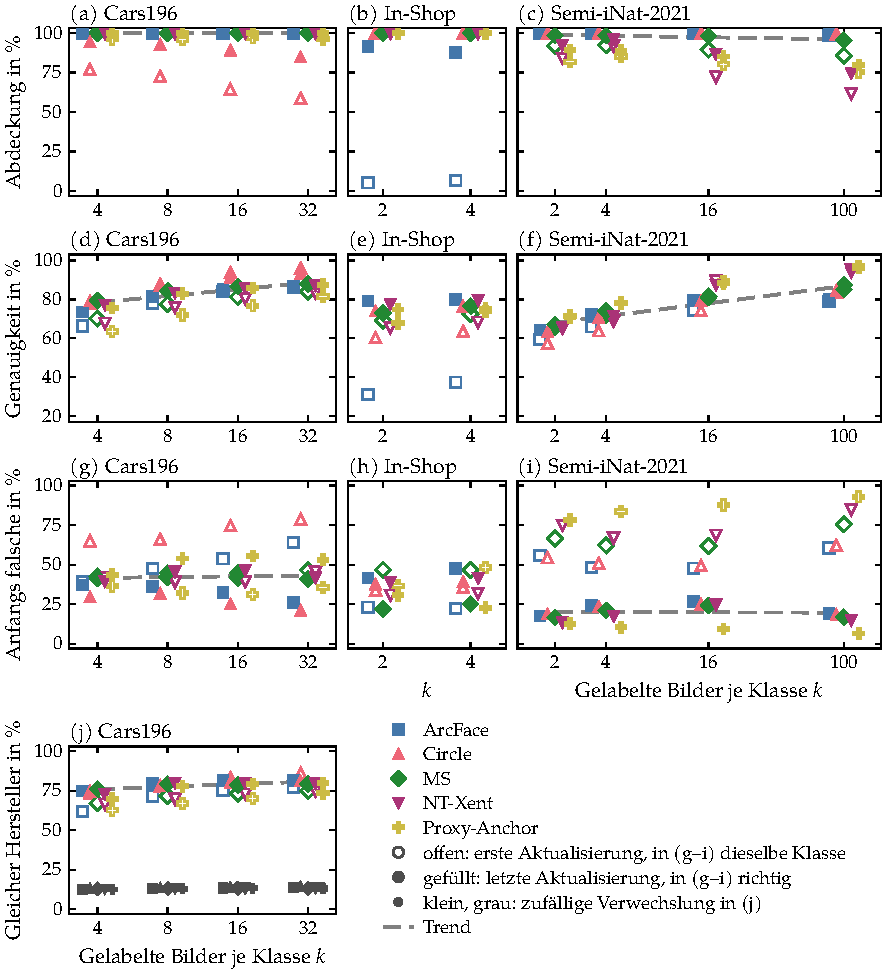
\includegraphics{neu/lp_pseudolabels}
  \caption[Pseudo-Labels von \acs{LP} über die Budgets]{Pseudo-Labels von \acs{LP} in den Geometrieläufen über das Label-Budget $k$, alle fünf Verlustfunktionen, Seed 2, Mittel über die vier Folds. (a--c) Abdeckung und (d--f) Genauigkeit der übernommenen Pseudo-Labels, offen bei der ersten, gefüllt bei der letzten Aktualisierung eines Folds. (g--i) Anteil der anfangs falschen Pseudo-Labels, die bei der letzten Aktualisierung richtig sind (gefüllt) oder noch dieselbe Klasse nennen (offen). (j) Anteil der falschen Pseudo-Labels, die ein Modell desselben Herstellers nennen, offen bei der ersten, gefüllt bei der letzten Aktualisierung, klein und grau bei zufälliger Verwechslung. Grau gestrichelt: Trend über die Verlustfunktionen (lineare Anpassung an den Median der gefüllten Punkte je Budget, auf In-Shop mit zwei Budgets ohne Trend).}
  \label{fig:e:lppseudolabels}
\end{figure}

\begingroup\small\setstretch{1}\setlength{\tabcolsep}{4pt}
\begin{longtable}{@{}>{\raggedright\arraybackslash\hangindent=2em\hangafter=1}p{5.1cm} *{5}{S[table-format=2.2]}@{}}
\caption[Alle Varianten der Phase 2 auf Cars196]{Alle Varianten der Phase 2 auf Cars196 ($k=16$, Seed 2): Test-MAP@R (Mean) in \%. Bezeichnungen wie in Tabelle \ref{tab:phase2:eingriffe} und Abschnitt \ref{sec:m:phase2}, Rauschschwelle $2\sqrt{2}\,\sigma$ in Prozentpunkten (Abschnitt \ref{sec:m:phase2}). Bei \acs{LRML} sind \enquote{ohne Warm-up} und \enquote{Warm-up $= 0$} dieselbe Einstellung. --: Lauf nicht vorhanden.}\label{tab:anhang:phase2}\\
\toprule
Variante & {ArcFace} & {Circle} & {\acs{MS}} & {NT-Xent} & {Proxy-Anchor} \\
\midrule
\endfirsthead
\multicolumn{6}{@{}l}{\small Tabelle \thetable{} (Fortsetzung)}\\
\toprule
Variante & {ArcFace} & {Circle} & {\acs{MS}} & {NT-Xent} & {Proxy-Anchor} \\
\midrule
\endhead
\bottomrule
\endlastfoot
\UEBL & 40.33 & 39.15 & 40.76 & 39.21 & 39.22 \\
\addlinespace
\multicolumn{6}{@{}l}{\textit{LP}} \\*
\quad Rauschschwelle & 0.8 & 0.5 & 0.6 & 0.6 & 0.3 \\
\quad reguläre Konfiguration & 41.95 & 42.28 & 43.30 & 41.37 & 42.60 \\
\quad Wiederholung mit Diagnose & 41.95 & 42.33 & 43.30 & 41.37 & 42.60 \\
\quad SSL-Mechanismus abgeschaltet & 37.45 & 39.04 & 40.56 & 39.19 & 39.94 \\
\quad Hyperparameter der \UEBL & 41.45 & 41.83 & 43.77 & 41.52 & 40.24 \\
\quad ohne Warm-up & 40.96 & 42.40 & 42.88 & 41.38 & 42.60 \\
\quad Pseudo-Labels eingefroren & 41.60 & 41.35 & 42.63 & 41.15 & 41.15 \\
\quad Graph umverdrahtet & 27.72 & 33.71 & 31.02 & 35.08 & 32.62 \\
\quad Oracle-Kanten entfernt & 41.70 & 43.14 & 43.85 & 42.53 & 43.61 \\
\quad zufällige Kanten entfernt & 41.81 & 42.48 & 42.92 & 41.56 & 42.66 \\
\quad Oracle-Labels, 0\,\% Rauschen & 42.09 & 42.91 & 44.17 & 42.42 & 43.55 \\
\quad Oracle-Labels, 10\,\% Rauschen & 42.53 & 37.83 & 41.89 & 42.29 & 41.18 \\
\quad Oracle-Labels, 20\,\% Rauschen & 42.07 & 37.03 & 39.20 & 41.33 & 39.10 \\
\quad Oracle-Labels, 40\,\% Rauschen & 40.21 & 36.18 & 33.74 & 39.06 & 36.21 \\
\quad Oracle-Labels, 60\,\% Rauschen & 38.71 & 35.51 & 31.89 & 36.11 & 33.36 \\
\quad Nachbarzahl $= 2$ & 41.32 & 42.22 & 42.92 & 41.52 & 42.63 \\
\quad Nachbarzahl $= 25$ & 41.62 & 42.34 & 42.69 & 41.26 & 42.66 \\
\quad Nachbarzahl $= 50$ & 41.29 & 42.30 & 42.25 & 41.27 & 42.68 \\
\quad Nachbarzahl $= 75$ & 41.65 & 42.09 & 42.21 & 41.03 & 42.67 \\
\quad Nachbarzahl $= 100$ & 41.61 & 42.10 & 41.68 & 40.71 & 42.55 \\
\quad Nachbarzahl $= 500$ & 41.59 & 39.96 & 38.90 & 40.66 & 37.14 \\
\quad Konfidenzschwelle $= 0{,}1$ & 41.95 & 42.30 & 43.13 & 41.37 & 42.57 \\
\quad Konfidenzschwelle $= 0{,}3$ & 41.95 & 42.30 & 43.13 & 41.37 & 42.57 \\
\quad Konfidenzschwelle $= 0{,}5$ & 41.70 & 42.29 & 43.06 & 41.59 & 42.46 \\
\quad Konfidenzschwelle $= 0{,}7$ & 41.52 & 42.45 & 43.01 & 41.73 & 42.50 \\
\quad Konfidenzschwelle $= 0{,}9$ & 39.23 & 41.67 & 40.89 & 41.14 & 42.68 \\
\quad Warm-up $= 30$ & 40.46 & 42.45 & 41.36 & 41.60 & 42.69 \\
\addlinespace
\multicolumn{6}{@{}l}{\textit{\acs{LRML}}} \\*
\quad Rauschschwelle & 0.5 & 0.7 & 1.1 & 0.7 & 0.5 \\
\quad reguläre Konfiguration & 40.91 & 40.89 & 40.37 & 39.85 & 41.72 \\
\quad SSL-Mechanismus abgeschaltet & 35.56 & 38.80 & 35.96 & 36.72 & 38.64 \\
\quad ohne ungelabelte Bilder & 37.79 & 40.49 & 38.48 & 39.19 & 40.58 \\
\quad Hyperparameter der \UEBL & 36.78 & 40.92 & 40.44 & 36.70 & 37.91 \\
\quad ohne Warm-up & 31.29 & 40.22 & 38.20 & 33.42 & 39.67 \\
\quad Graph eingefroren & 40.40 & 40.72 & 39.75 & 39.98 & 41.62 \\
\quad Graph umverdrahtet & 35.77 & 38.68 & 34.77 & 37.10 & 38.51 \\
\quad Oracle-Kanten entfernt & 41.30 & 41.36 & 41.13 & 40.46 & 42.45 \\
\quad zufällige Kanten entfernt & 41.08 & 40.94 & 40.10 & 40.14 & 41.67 \\
\quad Nachbarzahl $= 2$ & 39.60 & 38.98 & 37.46 & 39.46 & 40.57 \\
\quad Nachbarzahl $= 25$ & 41.05 & 40.38 & 39.99 & 39.69 & 41.58 \\
\quad Nachbarzahl $= 50$ & 41.01 & 40.60 & 40.35 & 39.89 & 41.61 \\
\quad Nachbarzahl $= 75$ & 40.66 & 41.03 & 40.16 & 40.24 & 41.63 \\
\quad Nachbarzahl $= 100$ & 40.03 & 41.10 & 39.67 & 40.07 & 41.21 \\
\quad Nachbarzahl $= 500$ & 37.32 & 40.43 & 35.45 & 39.19 & 40.13 \\
\quad $\eta$ $= 0{,}1$ & 36.16 & 39.25 & 36.32 & 36.96 & 39.02 \\
\quad $\eta$ $= 0{,}2$ & 36.99 & 39.58 & 36.90 & 37.27 & 39.41 \\
\quad $\eta$ $= 0{,}35$ & 38.25 & 40.07 & 37.43 & 37.69 & 39.98 \\
\quad $\eta$ $= 0{,}5$ & 39.73 & 40.54 & 38.23 & 38.10 & 40.48 \\
\quad $\eta$ $= 0{,}75$ & 41.06 & 41.10 & 39.70 & 38.20 & 41.54 \\
\quad $\eta$ $= 1{,}0$ & 41.23 & 41.33 & 40.59 & 39.76 & 41.82 \\
\quad $\eta$ $= 1{,}5$ & 40.44 & 40.55 & 41.30 & 40.64 & 41.68 \\
\quad $\eta$ $= 3{,}0$ & 38.30 & 39.07 & 39.68 & 38.95 & 40.08 \\
\quad Warm-up $= 0$ & 31.29 & 40.22 & 38.20 & 33.42 & 39.67 \\
\quad Warm-up $= 30$ & 40.91 & 40.93 & 40.37 & 37.03 & 41.72 \\
\addlinespace
\multicolumn{6}{@{}l}{\textit{Hoffer}} \\*
\quad Rauschschwelle & 0.3 & 0.4 & 0.5 & 0.7 & 0.5 \\
\quad reguläre Konfiguration & 40.52 & 40.62 & 39.47 & 40.31 & 40.65 \\
\quad SSL-Mechanismus abgeschaltet & 39.20 & 38.89 & 38.56 & 38.11 & 39.56 \\
\quad ohne ungelabelte Bilder & 38.26 & 39.30 & 38.46 & 38.51 & 39.39 \\
\quad Hyperparameter der \UEBL & 40.58 & 39.37 & 39.25 & 39.63 & 39.02 \\
\quad ohne Warm-up & 40.21 & 39.63 & 38.88 & 40.15 & 40.64 \\
\quad $\eta$ $= 0{,}1$ & 40.02 & 39.39 & 38.85 & 38.43 & 39.80 \\
\quad $\eta$ $= 0{,}2$ & 40.43 & 39.77 & 39.10 & 39.48 & 39.98 \\
\quad $\eta$ $= 0{,}35$ & 40.64 & 40.23 & 39.34 & 39.90 & 40.29 \\
\quad $\eta$ $= 0{,}5$ & 40.68 & 40.50 & 39.43 & 40.08 & 40.49 \\
\quad $\eta$ $= 0{,}75$ & 40.30 & 40.64 & 39.54 & 40.16 & 40.85 \\
\quad $\eta$ $= 1{,}0$ & 39.73 & 40.52 & 39.60 & 40.45 & 40.93 \\
\quad $\eta$ $= 1{,}5$ & 38.90 & 40.33 & 39.46 & 40.26 & 41.04 \\
\quad $\eta$ $= 3{,}0$ & 39.14 & 40.28 & 39.39 & 40.19 & 39.87 \\
\quad Distanzskala $\gamma_{\mathrm{H}}$ $= 1$ & 33.78 & 35.48 & 38.00 & 33.32 & 37.05 \\
\quad Distanzskala $\gamma_{\mathrm{H}}$ $= 2$ & 35.21 & 39.65 & 38.45 & 36.40 & 37.17 \\
\quad Distanzskala $\gamma_{\mathrm{H}}$ $= 4$ & 38.10 & 40.53 & 38.76 & 39.22 & 40.92 \\
\quad Distanzskala $\gamma_{\mathrm{H}}$ $= 16$ & 40.29 & 39.54 & 39.64 & 38.72 & 40.40 \\
\quad Distanzskala $\gamma_{\mathrm{H}}$ $= 32$ & 39.88 & 39.02 & 39.22 & 37.95 & 40.06 \\
\quad Distanzskala $\gamma_{\mathrm{H}}$ $= 64$ & 39.57 & 38.90 & 38.90 & 37.59 & 39.89 \\
\quad Distanzskala $\gamma_{\mathrm{H}}$ $= 128$ & 39.47 & 38.80 & 38.48 & 37.61 & 39.69 \\
\quad Distanzskala $\gamma_{\mathrm{H}}$ $= 256$ & 39.52 & 38.69 & 38.50 & 37.55 & 39.65 \\
\quad Distanzskala $\gamma_{\mathrm{H}}$ $= 512$ & 39.47 & 38.81 & 38.41 & 37.37 & 39.77 \\
\addlinespace
\multicolumn{6}{@{}l}{\textit{SLADE}} \\*
\quad Rauschschwelle & 1.0 & 0.6 & 1.0 & 0.3 & 0.6 \\
\quad reguläre Konfiguration & 40.20 & 41.60 & 41.68 & 40.61 & 40.38 \\
\quad SSL-Mechanismus abgeschaltet & 39.50 & 38.55 & 40.16 & 38.31 & 38.86 \\
\quad ohne ungelabelte Bilder & 40.04 & 38.12 & 40.84 & 38.79 & 39.52 \\
\quad Hyperparameter der \UEBL & 35.65 & 41.07 & 38.87 & 35.33 & 38.24 \\
\quad ohne Warm-up & 38.97 & 39.53 & 41.23 & 39.16 & 40.38 \\
\end{longtable}\endgroup

\begingroup\small\setstretch{1}\setlength{\tabcolsep}{4pt}
\begin{longtable}{@{}>{\raggedright\arraybackslash\hangindent=2em\hangafter=1}p{5.1cm} *{5}{S[table-format=2.2]}@{}}
\caption[Alle Varianten der Phase~2 auf In-Shop]{Alle Varianten der Phase~2 auf In-Shop ($k=2$, Seed~2), aufgebaut wie Tabelle~\ref{tab:anhang:phase2}. Fehlende SLADE-Werte: nicht untersucht, Sweeps in Tabelle~\ref{tab:anhang:phase2:slade}. --: Lauf nicht vorhanden.}\label{tab:anhang:phase2:inshop}\\
\toprule
Variante & {ArcFace} & {Circle} & {\acs{MS}} & {NT-Xent} & {Proxy-Anchor} \\
\midrule
\endfirsthead
\multicolumn{6}{@{}l}{\small Tabelle~\thetable{} (Fortsetzung)}\\
\toprule
Variante & {ArcFace} & {Circle} & {\acs{MS}} & {NT-Xent} & {Proxy-Anchor} \\
\midrule
\endhead
\bottomrule
\endlastfoot
\UEBL & 54.80 & 54.70 & 56.09 & 54.60 & 53.81 \\
\addlinespace
\multicolumn{6}{@{}l}{\textit{LP}} \\*
\quad Rauschschwelle & 0.1 & 0.3 & 0.2 & 0.4 & 0.4 \\
\quad reguläre Konfiguration & 58.91 & 57.76 & 58.81 & 57.95 & 56.30 \\
\quad Wiederholung mit Diagnose & 58.91 & 57.77 & 58.81 & 57.95 & 56.30 \\
\quad SSL-Term abgeschaltet & 48.12 & 54.64 & 55.77 & 53.73 & 52.87 \\
\quad ohne ungelabelte Bilder & 52.22 & 54.54 & 55.80 & 53.70 & 52.92 \\
\quad Hyperparameter der \UEBL & 58.21 & 56.72 & 58.98 & 57.28 & 53.71 \\
\quad ohne Warm-up & 58.79 & 57.64 & 59.00 & 57.82 & 55.87 \\
\quad Pseudo-Labels eingefroren & 47.43 & 55.21 & 58.16 & 55.80 & 55.00 \\
\quad Graph umverdrahtet & 45.51 & 47.59 & 49.35 & 46.47 & 47.36 \\
\quad Oracle-Kanten entfernt & 50.69 & 59.92 & 60.17 & 59.62 & 58.32 \\
\quad zufällige Kanten entfernt & 36.27 & 53.67 & 58.98 & 58.04 & 56.20 \\
\quad Oracle-Labels, 0\,\% Rauschen & 60.81 & 59.73 & 60.40 & 59.61 & 58.98 \\
\quad Oracle-Labels, 10\,\% Rauschen & 59.42 & 55.84 & 57.31 & 55.07 & 56.90 \\
\quad Oracle-Labels, 20\,\% Rauschen & 57.79 & 53.68 & 54.08 & 52.59 & 55.11 \\
\quad Oracle-Labels, 40\,\% Rauschen & 53.56 & 50.31 & 50.98 & 49.34 & 51.79 \\
\quad Oracle-Labels, 60\,\% Rauschen & 48.42 & 47.87 & 50.07 & 47.06 & 49.07 \\
\quad Nachbarzahl $= 2$ & 42.74 & 58.49 & 59.23 & 57.95 & 56.30 \\
\quad Nachbarzahl $= 25$ & 37.77 & 57.71 & 58.61 & 57.54 & 54.50 \\
\quad Nachbarzahl $= 50$ & 37.04 & 57.79 & 58.60 & 55.87 & 54.45 \\
\quad Nachbarzahl $= 75$ & 58.76 & 57.70 & 58.64 & 54.21 & 54.34 \\
\quad Nachbarzahl $= 100$ & 58.93 & 57.78 & 58.79 & 53.49 & 54.45 \\
\quad Nachbarzahl $= 500$ & 57.70 & 57.79 & 58.59 & 52.96 & 54.67 \\
\quad Konfidenzschwelle $= 0{,}1$ & 37.15 & 57.77 & 58.81 & 57.95 & 56.30 \\
\quad Konfidenzschwelle $= 0{,}3$ & 37.15 & 57.77 & 58.81 & 57.95 & 56.30 \\
\quad Konfidenzschwelle $= 0{,}5$ & 37.19 & 57.71 & 58.81 & 57.95 & 56.30 \\
\quad Konfidenzschwelle $= 0{,}7$ & 36.41 & 54.81 & 58.85 & 57.77 & 56.23 \\
\quad Konfidenzschwelle $= 0{,}9$ & 29.48 & 54.14 & 58.80 & 58.18 & 56.82 \\
\quad Warm-up $= 30$ & 58.89 & 57.85 & 58.82 & 57.94 & 56.30 \\
\addlinespace
\multicolumn{6}{@{}l}{\textit{\acs{LRML}}} \\*
\quad Rauschschwelle & 1.3 & 0.3 & 0.7 & 0.4 & 0.7 \\
\quad reguläre Konfiguration & 58.03 & 57.58 & 56.57 & 55.72 & 53.68 \\
\quad SSL-Term abgeschaltet & 47.00 & 52.95 & 54.11 & 53.17 & 50.97 \\
\quad ohne ungelabelte Bilder & 54.74 & 53.46 & 53.80 & 53.23 & 51.42 \\
\quad Hyperparameter der \UEBL & 52.42 & 56.00 & 57.17 & 54.68 & 54.07 \\
\quad ohne Warm-up & 49.60 & 57.30 & 56.23 & 55.66 & 54.36 \\
\quad Graph eingefroren & 56.70 & 55.75 & 56.37 & 55.40 & 51.36 \\
\quad Graph umverdrahtet & 46.63 & 45.94 & 52.17 & 50.82 & 51.12 \\
\quad Oracle-Kanten entfernt & 59.22 & 58.94 & 57.47 & 56.97 & 54.39 \\
\quad zufällige Kanten entfernt & 57.95 & 57.47 & 56.66 & 55.80 & 53.83 \\
\quad Nachbarzahl $= 2$ & 57.70 & 57.48 & 56.57 & 55.93 & 53.90 \\
\quad Nachbarzahl $= 25$ & 53.39 & 52.91 & 53.86 & 53.49 & 51.93 \\
\quad Nachbarzahl $= 50$ & 52.00 & 51.05 & 53.64 & 53.18 & 51.47 \\
\quad Nachbarzahl $= 75$ & 51.36 & 50.86 & 53.73 & 53.11 & 51.58 \\
\quad Nachbarzahl $= 100$ & 50.84 & 50.94 & 53.73 & 53.17 & 51.48 \\
\quad Nachbarzahl $= 500$ & 48.84 & 49.08 & 53.69 & 53.23 & 51.50 \\
\quad $\eta$ $= 0{,}1$ & 48.67 & 53.99 & 54.59 & 53.98 & 51.58 \\
\quad $\eta$ $= 0{,}2$ & 50.77 & 55.18 & 55.19 & 54.66 & 52.20 \\
\quad $\eta$ $= 0{,}35$ & 54.37 & 56.68 & 56.06 & 55.46 & 52.96 \\
\quad $\eta$ $= 0{,}5$ & 57.36 & 57.75 & 56.63 & 55.85 & 53.68 \\
\quad $\eta$ $= 0{,}75$ & 56.77 & 47.73 & 53.44 & 55.55 & 54.34 \\
\quad $\eta$ $= 1{,}0$ & 50.22 & 46.62 & 51.29 & 52.25 & 54.66 \\
\quad $\eta$ $= 1{,}5$ & 46.35 & 44.87 & 50.17 & 50.02 & 52.10 \\
\quad $\eta$ $= 3{,}0$ & 43.00 & 44.91 & 48.59 & 45.11 & 33.63 \\
\quad Warm-up $= 0$ & 49.60 & 57.30 & 56.23 & 55.66 & 54.36 \\
\quad Warm-up $= 30$ & 58.03 & 57.72 & 56.71 & 55.87 & 53.85 \\
\addlinespace
\multicolumn{6}{@{}l}{\textit{Hoffer}} \\*
\quad Rauschschwelle & 0.2 & 0.2 & 0.2 & 0.2 & 0.3 \\
\quad reguläre Konfiguration & 57.75 & 58.05 & 57.90 & 58.21 & 57.56 \\
\quad SSL-Term abgeschaltet & 52.70 & 54.35 & 53.05 & 51.96 & 51.88 \\
\quad ohne ungelabelte Bilder & 53.62 & 54.49 & 53.89 & 54.70 & 53.60 \\
\quad Hyperparameter der \UEBL & 57.19 & 57.50 & 56.97 & 57.11 & 56.60 \\
\quad ohne Warm-up & 57.24 & 57.98 & 57.68 & 58.05 & 57.56 \\
\quad $\eta$ $= 0{,}1$ & 54.06 & 54.82 & 54.69 & 54.17 & 53.25 \\
\quad $\eta$ $= 0{,}2$ & 55.03 & 55.37 & 55.78 & 55.58 & 54.32 \\
\quad $\eta$ $= 0{,}35$ & 56.10 & 55.97 & 56.62 & 56.91 & 55.51 \\
\quad $\eta$ $= 0{,}5$ & 56.67 & 56.53 & 57.12 & 57.59 & 56.25 \\
\quad $\eta$ $= 0{,}75$ & 57.34 & 57.29 & 57.54 & 58.12 & 56.92 \\
\quad $\eta$ $= 1{,}0$ & 57.67 & 57.68 & 57.73 & 58.30 & 57.36 \\
\quad $\eta$ $= 1{,}5$ & 57.75 & 57.98 & 58.02 & 58.32 & 57.60 \\
\quad $\eta$ $= 3{,}0$ & 56.95 & 57.67 & 58.13 & 58.01 & 56.93 \\
\quad Distanzskala $\gamma_{\mathrm{H}}$ $= 1$ & 33.53 & 40.94 & 34.15 & 38.65 & 13.21 \\
\quad Distanzskala $\gamma_{\mathrm{H}}$ $= 2$ & 30.34 & 35.91 & 34.47 & 41.68 & 6.15 \\
\quad Distanzskala $\gamma_{\mathrm{H}}$ $= 4$ & 38.94 & 43.85 & 44.29 & 44.81 & 16.37 \\
\quad Distanzskala $\gamma_{\mathrm{H}}$ $= 16$ & 56.95 & 56.43 & 57.06 & 57.41 & 56.83 \\
\quad Distanzskala $\gamma_{\mathrm{H}}$ $= 32$ & 55.10 & 55.12 & 54.80 & 55.10 & 54.97 \\
\quad Distanzskala $\gamma_{\mathrm{H}}$ $= 64$ & 53.53 & 54.46 & 53.23 & 53.02 & 52.90 \\
\quad Distanzskala $\gamma_{\mathrm{H}}$ $= 128$ & 52.68 & 54.17 & 52.86 & 52.20 & 51.29 \\
\quad Distanzskala $\gamma_{\mathrm{H}}$ $= 256$ & 52.26 & 54.10 & 52.72 & 52.03 & 50.61 \\
\quad Distanzskala $\gamma_{\mathrm{H}}$ $= 512$ & 51.96 & 54.05 & 52.67 & 51.93 & 50.24 \\
\addlinespace
\multicolumn{6}{@{}l}{\textit{SLADE}} \\*
\quad Rauschschwelle & 1.4 & 0.4 & 0.4 & 0.5 & 0.9 \\
\quad reguläre Konfiguration & 53.69 & 54.77 & 54.49 & 54.14 & 53.71 \\
\quad SSL-Term abgeschaltet & 52.66 & 54.71 & 52.65 & 54.16 & 43.10 \\
\quad ohne ungelabelte Bilder & 54.03 & 54.49 & 53.98 & 54.22 & 53.71 \\
\quad Hyperparameter der \UEBL & 46.61 & 53.39 & 51.05 & 53.86 & 52.14 \\
\quad ohne Warm-up & 53.69 & 54.56 & 54.35 & 54.27 & 53.65 \\
\end{longtable}\endgroup

\begingroup\small\setstretch{1}\setlength{\tabcolsep}{4pt}
\begin{longtable}{@{}>{\raggedright\arraybackslash\hangindent=2em\hangafter=1}p{5.1cm} *{5}{S[table-format=2.2]}@{}}
\caption[Alle Varianten der Phase~2 auf Cars196 als Ensemble]{Alle Varianten der Phase~2 auf Cars196 wie in Tabelle~\ref{tab:anhang:phase2}, aber für das Ensemble (Test-MAP@R Concat in \%). Rauschschwelle aus der Seed-Standardabweichung der Concat-MAP@R in Phase~1 (Abschnitt~\ref{sec:m:phase2}).}\label{tab:anhang:phase2:concat}\\
\toprule
Variante & {ArcFace} & {Circle} & {\acs{MS}} & {NT-Xent} & {Proxy-Anchor} \\
\midrule
\endfirsthead
\multicolumn{6}{@{}l}{\small Tabelle~\thetable{} (Fortsetzung)}\\
\toprule
Variante & {ArcFace} & {Circle} & {\acs{MS}} & {NT-Xent} & {Proxy-Anchor} \\
\midrule
\endhead
\bottomrule
\endlastfoot
\UEBL & 43.41 & 42.66 & 44.20 & 42.53 & 42.84 \\
Rauschschwelle \UEBL & 0.7 & 0.5 & 0.6 & 0.7 & 0.9 \\
\addlinespace
\multicolumn{6}{@{}l}{\textit{LP}} \\*
\quad Rauschschwelle & 0.5 & 0.6 & 0.3 & 0.3 & 0.3 \\
\quad reguläre Konfiguration & 44.59 & 44.65 & 46.23 & 44.29 & 45.06 \\
\quad Wiederholung mit Diagnose & 44.59 & 44.72 & 46.23 & 44.29 & 45.06 \\
\quad SSL-Term abgeschaltet & 41.61 & 41.99 & 43.92 & 42.50 & 42.87 \\
\quad ohne ungelabelte Bilder & 41.45 & 42.02 & 44.18 & 42.55 & 42.96 \\
\quad Hyperparameter der \UEBL & 43.96 & 44.88 & 45.92 & 44.22 & 44.16 \\
\quad ohne Warm-up & 43.78 & 44.92 & 46.08 & 44.21 & 45.05 \\
\quad Pseudo-Labels eingefroren & 44.36 & 44.14 & 45.85 & 43.95 & 43.82 \\
\quad Graph umverdrahtet & 30.98 & 35.39 & 32.09 & 36.23 & 32.93 \\
\quad Oracle-Kanten entfernt & 44.49 & 45.13 & 46.67 & 44.82 & 45.59 \\
\quad zufällige Kanten entfernt & 44.49 & 44.89 & 45.94 & 44.35 & 45.17 \\
\quad Oracle-Labels, 0\,\% Rauschen & 44.72 & 45.18 & 46.78 & 44.82 & 45.56 \\
\quad Oracle-Labels, 10\,\% Rauschen & 45.12 & 38.96 & 45.04 & 44.64 & 44.23 \\
\quad Oracle-Labels, 20\,\% Rauschen & 44.93 & 38.12 & 42.33 & 44.09 & 42.23 \\
\quad Oracle-Labels, 40\,\% Rauschen & 44.12 & 37.21 & 36.43 & 41.57 & 38.64 \\
\quad Oracle-Labels, 60\,\% Rauschen & 42.67 & 36.54 & 33.00 & 38.01 & 34.75 \\
\quad Nachbarzahl $= 2$ & 44.28 & 44.72 & 46.14 & 44.40 & 45.16 \\
\quad Nachbarzahl $= 25$ & 44.47 & 44.85 & 45.82 & 44.20 & 45.15 \\
\quad Nachbarzahl $= 50$ & 44.12 & 44.88 & 45.53 & 44.08 & 45.05 \\
\quad Nachbarzahl $= 75$ & 44.35 & 44.92 & 45.37 & 43.84 & 45.00 \\
\quad Nachbarzahl $= 100$ & 44.23 & 44.88 & 44.96 & 43.61 & 44.93 \\
\quad Nachbarzahl $= 500$ & 44.34 & 43.10 & 40.36 & 43.48 & 40.09 \\
\quad Konfidenzschwelle $= 0{,}1$ & 44.59 & 44.80 & 46.16 & 44.29 & 45.07 \\
\quad Konfidenzschwelle $= 0{,}3$ & 44.59 & 44.80 & 46.16 & 44.29 & 45.07 \\
\quad Konfidenzschwelle $= 0{,}5$ & 44.32 & 44.74 & 46.08 & 44.30 & 45.06 \\
\quad Konfidenzschwelle $= 0{,}7$ & 44.41 & 44.77 & 46.09 & 44.42 & 45.10 \\
\quad Konfidenzschwelle $= 0{,}9$ & 43.19 & 44.59 & 45.14 & 44.34 & 45.10 \\
\quad Warm-up $= 30$ & 43.81 & 44.94 & 45.52 & 44.42 & 45.10 \\
\addlinespace
\multicolumn{6}{@{}l}{\textit{\acs{LRML}}} \\*
\quad Rauschschwelle & 0.7 & 0.7 & 0.6 & 0.8 & 0.3 \\
\quad reguläre Konfiguration & 44.39 & 44.48 & 45.20 & 43.97 & 45.22 \\
\quad SSL-Term abgeschaltet & 39.89 & 41.64 & 40.72 & 41.81 & 41.28 \\
\quad ohne ungelabelte Bilder & 41.38 & 43.38 & 43.39 & 43.57 & 42.71 \\
\quad Hyperparameter der \UEBL & 37.44 & 43.44 & 41.63 & 37.31 & 42.90 \\
\quad ohne Warm-up & 37.50 & 44.24 & 43.36 & 39.67 & 44.13 \\
\quad Graph eingefroren & 44.40 & 44.46 & 45.21 & 44.28 & 45.10 \\
\quad Graph umverdrahtet & 40.11 & 40.80 & 39.46 & 41.92 & 40.37 \\
\quad Oracle-Kanten entfernt & 44.83 & 45.03 & 45.67 & 44.31 & 45.55 \\
\quad zufällige Kanten entfernt & 44.47 & 44.46 & 45.12 & 44.05 & 45.20 \\
\quad Nachbarzahl $= 2$ & 42.64 & 42.54 & 41.44 & 43.45 & 44.27 \\
\quad Nachbarzahl $= 25$ & 44.30 & 44.09 & 44.63 & 43.77 & 45.14 \\
\quad Nachbarzahl $= 50$ & 44.45 & 44.38 & 45.16 & 43.99 & 45.22 \\
\quad Nachbarzahl $= 75$ & 44.25 & 44.43 & 45.13 & 44.20 & 45.19 \\
\quad Nachbarzahl $= 100$ & 43.71 & 44.27 & 44.99 & 44.10 & 44.74 \\
\quad Nachbarzahl $= 500$ & 41.44 & 43.01 & 41.74 & 43.85 & 42.46 \\
\quad $\eta$ $= 0{,}1$ & 40.59 & 42.17 & 41.49 & 42.14 & 41.72 \\
\quad $\eta$ $= 0{,}2$ & 41.48 & 43.04 & 42.98 & 42.37 & 42.08 \\
\quad $\eta$ $= 0{,}35$ & 42.87 & 43.97 & 43.62 & 42.75 & 42.83 \\
\quad $\eta$ $= 0{,}5$ & 43.93 & 44.39 & 44.34 & 43.14 & 43.59 \\
\quad $\eta$ $= 0{,}75$ & 44.49 & 44.35 & 45.13 & 43.57 & 44.70 \\
\quad $\eta$ $= 1{,}0$ & 43.90 & 43.30 & 45.37 & 43.88 & 45.27 \\
\quad $\eta$ $= 1{,}5$ & 42.98 & 42.37 & 44.99 & 43.92 & 43.28 \\
\quad $\eta$ $= 3{,}0$ & 40.58 & 40.62 & 43.06 & 41.50 & 41.30 \\
\quad Warm-up $= 0$ & 37.50 & 44.24 & 43.36 & 39.67 & 44.13 \\
\quad Warm-up $= 30$ & 44.39 & 44.63 & 45.20 & 42.89 & 45.22 \\
\addlinespace
\multicolumn{6}{@{}l}{\textit{Hoffer}} \\*
\quad Rauschschwelle & 0.6 & 0.5 & 0.6 & 0.7 & 0.6 \\
\quad reguläre Konfiguration & 44.13 & 44.34 & 43.46 & 44.22 & 44.03 \\
\quad SSL-Term abgeschaltet & 42.49 & 41.82 & 42.08 & 40.16 & 42.75 \\
\quad ohne ungelabelte Bilder & 41.73 & 42.74 & 42.31 & 42.25 & 42.58 \\
\quad Hyperparameter der \UEBL & 44.16 & 43.36 & 43.43 & 43.72 & 43.41 \\
\quad ohne Warm-up & 44.02 & 43.88 & 43.10 & 44.06 & 43.89 \\
\quad $\eta$ $= 0{,}1$ & 43.40 & 42.67 & 42.79 & 41.71 & 43.03 \\
\quad $\eta$ $= 0{,}2$ & 43.82 & 43.51 & 43.13 & 43.06 & 43.33 \\
\quad $\eta$ $= 0{,}35$ & 44.12 & 44.10 & 43.41 & 43.65 & 43.62 \\
\quad $\eta$ $= 0{,}5$ & 44.18 & 44.27 & 43.50 & 43.89 & 43.89 \\
\quad $\eta$ $= 0{,}75$ & 44.07 & 44.36 & 43.55 & 44.12 & 44.15 \\
\quad $\eta$ $= 1{,}0$ & 43.78 & 44.28 & 43.51 & 44.21 & 44.26 \\
\quad $\eta$ $= 1{,}5$ & 43.24 & 44.14 & 43.44 & 44.22 & 44.21 \\
\quad $\eta$ $= 3{,}0$ & 42.90 & 43.93 & 43.57 & 44.20 & 43.74 \\
\quad Distanzskala $\gamma_{\mathrm{H}}$ $= 1$ & 34.59 & 37.93 & 39.44 & 34.79 & 40.16 \\
\quad Distanzskala $\gamma_{\mathrm{H}}$ $= 2$ & 35.94 & 41.82 & 39.98 & 37.96 & 39.48 \\
\quad Distanzskala $\gamma_{\mathrm{H}}$ $= 4$ & 42.42 & 44.39 & 43.07 & 43.49 & 43.96 \\
\quad Distanzskala $\gamma_{\mathrm{H}}$ $= 16$ & 43.68 & 42.74 & 43.03 & 41.83 & 43.74 \\
\quad Distanzskala $\gamma_{\mathrm{H}}$ $= 32$ & 43.34 & 42.53 & 42.72 & 41.00 & 43.32 \\
\quad Distanzskala $\gamma_{\mathrm{H}}$ $= 64$ & 43.00 & 42.19 & 42.25 & 40.61 & 42.98 \\
\quad Distanzskala $\gamma_{\mathrm{H}}$ $= 128$ & 42.79 & 42.09 & 42.17 & 40.75 & 42.89 \\
\quad Distanzskala $\gamma_{\mathrm{H}}$ $= 256$ & 42.68 & 41.90 & 42.08 & 40.20 & 42.83 \\
\quad Distanzskala $\gamma_{\mathrm{H}}$ $= 512$ & 42.63 & 41.76 & 41.96 & 40.19 & 42.83 \\
\addlinespace
\multicolumn{6}{@{}l}{\textit{SLADE}} \\*
\quad Rauschschwelle & 0.7 & 0.7 & 0.7 & 0.7 & 0.6 \\
\quad reguläre Konfiguration & 43.51 & 44.91 & 44.95 & 44.26 & 43.62 \\
\quad SSL-Term abgeschaltet & 42.73 & 41.52 & 43.38 & 41.36 & 41.41 \\
\quad ohne ungelabelte Bilder & 42.34 & 43.03 & 44.42 & 42.58 & 42.62 \\
\quad Hyperparameter der \UEBL & 39.44 & 43.52 & 43.27 & 39.81 & 42.66 \\
\quad ohne Warm-up & 42.77 & 43.36 & 44.37 & 43.59 & 43.62 \\
\end{longtable}\endgroup

\begingroup\small\setstretch{1}\setlength{\tabcolsep}{4pt}
\begin{longtable}{@{}>{\raggedright\arraybackslash\hangindent=2em\hangafter=1}p{5.1cm} *{5}{S[table-format=2.2]}@{}}
\caption[Alle Varianten der Phase~2 auf In-Shop als Ensemble]{Alle Varianten der Phase~2 auf In-Shop wie in Tabelle~\ref{tab:anhang:phase2:inshop}, aber für das Ensemble (Test-MAP@R Concat in \%). Rauschschwelle aus der Seed-Standardabweichung der Concat-MAP@R in Phase~1 (Abschnitt~\ref{sec:m:phase2}).}\label{tab:anhang:phase2:inshop:concat}\\
\toprule
Variante & {ArcFace} & {Circle} & {\acs{MS}} & {NT-Xent} & {Proxy-Anchor} \\
\midrule
\endfirsthead
\multicolumn{6}{@{}l}{\small Tabelle~\thetable{} (Fortsetzung)}\\
\toprule
Variante & {ArcFace} & {Circle} & {\acs{MS}} & {NT-Xent} & {Proxy-Anchor} \\
\midrule
\endhead
\bottomrule
\endlastfoot
\UEBL & 57.45 & 57.61 & 58.84 & 57.29 & 55.97 \\
Rauschschwelle \UEBL & 0.2 & 0.6 & 0.4 & 0.3 & 0.4 \\
\addlinespace
\multicolumn{6}{@{}l}{\textit{LP}} \\*
\quad Rauschschwelle & 0.1 & 0.3 & 0.4 & 0.6 & 0.5 \\
\quad reguläre Konfiguration & 60.62 & 60.06 & 61.08 & 60.23 & 57.22 \\
\quad Wiederholung mit Diagnose & 60.62 & 60.01 & 61.08 & 60.23 & 57.22 \\
\quad SSL-Term abgeschaltet & 50.90 & 57.59 & 59.05 & 56.62 & 54.80 \\
\quad ohne ungelabelte Bilder & 55.76 & 57.49 & 58.80 & 56.50 & 54.91 \\
\quad Hyperparameter der \UEBL & 59.41 & 59.03 & 60.96 & 58.92 & 54.97 \\
\quad ohne Warm-up & 60.53 & 59.90 & 61.35 & 59.93 & 56.88 \\
\quad Pseudo-Labels eingefroren & 52.04 & 57.35 & 60.34 & 57.91 & 56.02 \\
\quad Graph umverdrahtet & 48.44 & 49.10 & 50.74 & 48.68 & 48.21 \\
\quad Oracle-Kanten entfernt & 51.88 & 61.79 & 62.19 & 61.62 & 59.20 \\
\quad zufällige Kanten entfernt & 37.77 & 55.74 & 61.21 & 60.10 & 57.12 \\
\quad Oracle-Labels, 0\,\% Rauschen & 62.04 & 61.36 & 62.55 & 61.35 & 59.73 \\
\quad Oracle-Labels, 10\,\% Rauschen & 61.27 & 58.49 & 60.01 & 57.47 & 58.42 \\
\quad Oracle-Labels, 20\,\% Rauschen & 60.30 & 56.49 & 56.56 & 55.04 & 57.44 \\
\quad Oracle-Labels, 40\,\% Rauschen & 57.20 & 52.96 & 52.25 & 51.53 & 53.93 \\
\quad Oracle-Labels, 60\,\% Rauschen & 53.00 & 50.28 & 51.44 & 49.43 & 50.50 \\
\quad Nachbarzahl $= 2$ & 44.20 & 60.50 & 61.71 & 60.23 & 57.22 \\
\quad Nachbarzahl $= 25$ & 39.21 & 59.90 & 60.81 & 59.72 & 55.64 \\
\quad Nachbarzahl $= 50$ & 38.67 & 59.99 & 60.96 & 58.56 & 55.73 \\
\quad Nachbarzahl $= 75$ & 60.54 & 59.87 & 61.08 & 56.90 & 55.44 \\
\quad Nachbarzahl $= 100$ & 60.56 & 60.08 & 61.25 & 56.65 & 55.60 \\
\quad Nachbarzahl $= 500$ & 59.87 & 60.02 & 60.72 & 56.21 & 55.85 \\
\quad Konfidenzschwelle $= 0{,}1$ & 38.61 & 60.01 & 61.08 & 60.23 & 57.22 \\
\quad Konfidenzschwelle $= 0{,}3$ & 38.61 & 60.01 & 61.08 & 60.23 & 57.22 \\
\quad Konfidenzschwelle $= 0{,}5$ & 38.73 & 59.72 & 61.08 & 60.23 & 57.22 \\
\quad Konfidenzschwelle $= 0{,}7$ & 57.07 & 57.72 & 61.19 & 59.84 & 57.11 \\
\quad Konfidenzschwelle $= 0{,}9$ & 33.60 & 57.37 & 61.11 & 60.34 & 57.67 \\
\quad Warm-up $= 30$ & 60.51 & 60.06 & 61.09 & 60.10 & 57.16 \\
\addlinespace
\multicolumn{6}{@{}l}{\textit{\acs{LRML}}} \\*
\quad Rauschschwelle & 1.3 & 0.3 & 0.7 & 0.7 & 0.5 \\
\quad reguläre Konfiguration & 60.14 & 59.26 & 59.60 & 59.44 & 55.93 \\
\quad SSL-Term abgeschaltet & 49.33 & 55.26 & 57.44 & 56.30 & 53.98 \\
\quad ohne ungelabelte Bilder & 57.53 & 56.25 & 56.75 & 57.04 & 54.16 \\
\quad Hyperparameter der \UEBL & 53.28 & 58.10 & 59.46 & 57.28 & 56.32 \\
\quad ohne Warm-up & 51.14 & 59.40 & 59.63 & 59.46 & 55.97 \\
\quad Graph eingefroren & 59.46 & 57.37 & 59.23 & 58.73 & 53.74 \\
\quad Graph umverdrahtet & 48.82 & 46.56 & 54.85 & 53.23 & 53.98 \\
\quad Oracle-Kanten entfernt & 61.26 & 60.47 & 60.31 & 60.40 & 56.58 \\
\quad zufällige Kanten entfernt & 60.15 & 59.18 & 59.63 & 59.34 & 56.11 \\
\quad Nachbarzahl $= 2$ & 59.38 & 59.05 & 59.60 & 59.36 & 56.01 \\
\quad Nachbarzahl $= 25$ & 56.88 & 56.22 & 57.05 & 57.39 & 54.68 \\
\quad Nachbarzahl $= 50$ & 55.57 & 54.29 & 57.12 & 57.20 & 54.05 \\
\quad Nachbarzahl $= 75$ & 54.95 & 54.13 & 56.95 & 56.98 & 54.28 \\
\quad Nachbarzahl $= 100$ & 54.66 & 53.87 & 56.93 & 57.05 & 54.23 \\
\quad Nachbarzahl $= 500$ & 52.13 & 51.15 & 56.83 & 57.19 & 54.33 \\
\quad $\eta$ $= 0{,}1$ & 51.58 & 56.33 & 57.72 & 57.39 & 54.52 \\
\quad $\eta$ $= 0{,}2$ & 53.91 & 57.64 & 58.48 & 58.36 & 54.89 \\
\quad $\eta$ $= 0{,}35$ & 57.69 & 58.85 & 59.50 & 59.12 & 55.45 \\
\quad $\eta$ $= 0{,}5$ & 60.28 & 59.70 & 59.74 & 59.41 & 55.99 \\
\quad $\eta$ $= 0{,}75$ & 58.80 & 48.40 & 56.37 & 59.19 & 56.16 \\
\quad $\eta$ $= 1{,}0$ & 51.87 & 47.35 & 52.36 & 55.11 & 56.33 \\
\quad $\eta$ $= 1{,}5$ & 47.33 & 45.22 & 51.27 & 51.66 & 53.59 \\
\quad $\eta$ $= 3{,}0$ & 44.33 & 45.30 & 49.62 & 46.51 & 37.03 \\
\quad Warm-up $= 0$ & 51.14 & 59.40 & 59.63 & 59.46 & 55.97 \\
\quad Warm-up $= 30$ & 60.14 & 59.44 & 59.79 & 59.57 & 56.13 \\
\addlinespace
\multicolumn{6}{@{}l}{\textit{Hoffer}} \\*
\quad Rauschschwelle & 0.4 & 0.3 & 0.3 & 0.5 & 0.2 \\
\quad reguläre Konfiguration & 60.35 & 60.37 & 60.66 & 60.78 & 60.00 \\
\quad SSL-Term abgeschaltet & 55.89 & 57.20 & 56.77 & 55.87 & 54.60 \\
\quad ohne ungelabelte Bilder & 56.82 & 57.09 & 57.04 & 57.97 & 57.41 \\
\quad Hyperparameter der \UEBL & 59.66 & 59.65 & 59.50 & 59.23 & 58.37 \\
\quad ohne Warm-up & 60.00 & 60.20 & 60.61 & 60.38 & 60.00 \\
\quad $\eta$ $= 0{,}1$ & 56.95 & 57.81 & 58.52 & 57.72 & 55.85 \\
\quad $\eta$ $= 0{,}2$ & 57.93 & 58.38 & 59.24 & 58.91 & 56.80 \\
\quad $\eta$ $= 0{,}35$ & 58.64 & 58.96 & 59.87 & 59.89 & 57.76 \\
\quad $\eta$ $= 0{,}5$ & 59.57 & 59.38 & 60.14 & 60.25 & 58.51 \\
\quad $\eta$ $= 0{,}75$ & 59.98 & 59.96 & 60.47 & 60.71 & 59.34 \\
\quad $\eta$ $= 1{,}0$ & 60.31 & 60.09 & 60.51 & 60.73 & 59.82 \\
\quad $\eta$ $= 1{,}5$ & 60.34 & 60.13 & 60.61 & 60.50 & 60.09 \\
\quad $\eta$ $= 3{,}0$ & 59.65 & 59.64 & 60.81 & 60.01 & 59.65 \\
\quad Distanzskala $\gamma_{\mathrm{H}}$ $= 1$ & 34.47 & 45.09 & 35.95 & 39.76 & 8.48 \\
\quad Distanzskala $\gamma_{\mathrm{H}}$ $= 2$ & 31.44 & 38.87 & 36.04 & 42.91 & 6.43 \\
\quad Distanzskala $\gamma_{\mathrm{H}}$ $= 4$ & 39.89 & 46.06 & 45.59 & 45.95 & 20.23 \\
\quad Distanzskala $\gamma_{\mathrm{H}}$ $= 16$ & 60.10 & 59.18 & 60.13 & 60.29 & 59.51 \\
\quad Distanzskala $\gamma_{\mathrm{H}}$ $= 32$ & 58.32 & 58.15 & 58.43 & 58.57 & 57.37 \\
\quad Distanzskala $\gamma_{\mathrm{H}}$ $= 64$ & 56.74 & 57.46 & 56.67 & 56.43 & 55.26 \\
\quad Distanzskala $\gamma_{\mathrm{H}}$ $= 128$ & 55.79 & 57.21 & 56.65 & 55.57 & 53.64 \\
\quad Distanzskala $\gamma_{\mathrm{H}}$ $= 256$ & 55.49 & 56.96 & 56.60 & 55.56 & 53.07 \\
\quad Distanzskala $\gamma_{\mathrm{H}}$ $= 512$ & 55.10 & 57.07 & 56.46 & 55.40 & 52.61 \\
\addlinespace
\multicolumn{6}{@{}l}{\textit{SLADE}} \\*
\quad Rauschschwelle & 1.4 & 0.7 & 0.6 & 0.5 & 0.4 \\
\quad reguläre Konfiguration & 56.92 & 56.85 & 57.53 & 56.80 & 57.77 \\
\quad SSL-Term abgeschaltet & 54.98 & 57.29 & 55.49 & 57.18 & 49.90 \\
\quad ohne ungelabelte Bilder & 57.08 & 56.65 & 57.30 & 57.22 & 57.79 \\
\quad Hyperparameter der \UEBL & 49.57 & 55.55 & 52.13 & 55.93 & 54.38 \\
\quad ohne Warm-up & 56.92 & 56.61 & 57.34 & 56.99 & 57.94 \\
\end{longtable}\endgroup

\begin{table}[p]
\centering
\caption[Sweeps von SLADE in Phase 2]{Sweeps einzelner Hyperparameter von SLADE (Phase 2, Seed 2, Cars196 mit $k=16$, In-Shop mit $k=2$): Änderung der Test-MAP@R (Mean) gegenüber der regulären SLADE-Konfiguration in Prozentpunkten. Fett: Betrag über der Rauschschwelle $2\sqrt{2}\,\sigma$, kursiv: in Phase 1 gewählter Wert (Wiederholung der regulären Konfiguration, bei der Teacher-Aktualisierung alle 5 Epochen die reguläre Konfiguration selbst). $^\dagger$: außerhalb der Suchräume der Phase 1 (Clusterverhältnis 0,5 nur auf Cars196). Arc: ArcFace, Cir: Circle, NT: NT-Xent, PA: Proxy-Anchor.}
\label{tab:anhang:phase2:slade}
\small\setlength{\tabcolsep}{3.2pt}
\begin{tabular}{@{}lrrrrrrrrrr@{}}
\toprule
 & \multicolumn{5}{c}{Cars196} & \multicolumn{5}{c}{In-Shop} \\
\cmidrule(lr){2-6}\cmidrule(lr){7-11}
Wert & Arc & Cir & \acs{MS} & NT & PA & Arc & Cir & \acs{MS} & NT & PA \\
\midrule
reguläre Konfiguration [\%] & 40{,}2 & 41{,}6 & 41{,}7 & 40{,}6 & 40{,}4 & 53{,}7 & 54{,}8 & 54{,}5 & 54{,}1 & 53{,}7 \\
Rauschschwelle & 1{,}0 & 0{,}6 & 1{,}0 & 0{,}3 & 0{,}6 & 1{,}4 & 0{,}4 & 0{,}4 & 0{,}5 & 0{,}9 \\
\addlinespace
\multicolumn{11}{@{}l}{\emph{Zielverhältnis $\eta$}} \\
\quad 0{,}1$^\dagger$ & \textminus 0{,}7 & \textbf{\textminus 2{,}9} & \textminus 0{,}8 & \textbf{\textminus 1{,}8} & \textminus 0{,}5 & +0{,}6 & \textminus 0{,}1 & \textbf{\textminus 0{,}9} & \textminus 0{,}1 & +0{,}1 \\
\quad 0{,}2$^\dagger$ & \textminus 0{,}5 & \textbf{\textminus 2{,}2} & \textminus 0{,}3 & \textbf{\textminus 1{,}5} & \textminus 0{,}1 & +0{,}2 & \textminus 0{,}1 & \textbf{\textminus 0{,}8} & \textminus 0{,}0 & \textminus 0{,}0 \\
\quad 0{,}5 & +0{,}1 & \textminus 0{,}6 & +0{,}1 & \textbf{\textminus 1{,}2} & +0{,}1 & +0{,}7 & \textminus 0{,}0 & \textbf{\textminus 0{,}4} & \textminus 0{,}0 & \textminus 0{,}0 \\
\quad 1 & \textminus 0{,}1 & +0{,}1 & \textminus 0{,}3 & \textbf{\textminus 0{,}5} & \textminus 0{,}6 & \textbf{\textminus 1{,}8} & \textbf{\textminus 1{,}5} & \textminus 0{,}0 & \textminus 0{,}3 & \textminus 0{,}6 \\
\quad 1{,}5 & +0{,}2 & \textbf{\textminus 2{,}4} & +0{,}2 & \textminus 0{,}1 & \textbf{\textminus 0{,}8} & \textbf{\textminus 2{,}5} & \textbf{\textminus 6{,}9} & +0{,}2 & \textbf{\textminus 0{,}6} & \textbf{\textminus 1{,}9} \\
\quad 3$^\dagger$ & \textminus 0{,}3 & \textbf{\textminus 8{,}6} & \textbf{\textminus 1{,}1} & \textbf{\textminus 0{,}4} & \textbf{\textminus 1{,}4} & \textbf{\textminus 3{,}5} & \textbf{\textminus 9{,}8} & \textbf{\textminus 3{,}6} & \textbf{\textminus 2{,}6} & \textbf{\textminus 1{,}6} \\
\addlinespace
\multicolumn{11}{@{}l}{\emph{Basis: Zielverhältnis $\eta_{\mathrm{basis}}$}} \\
\quad 0{,}1$^\dagger$ & +0{,}2 & \textbf{\textminus 0{,}9} & \textminus 0{,}1 & \textbf{\textminus 1{,}7} & \textminus 0{,}2 & \textbf{\textminus 4{,}5} & +0{,}3 & \textbf{\textminus 0{,}7} & +0{,}2 & \textbf{\textminus 16{,}6} \\
\quad 1 & \textminus 0{,}1 & +0{,}1 & +0{,}3 & \textminus 0{,}1 & \textminus 0{,}3 & \textminus 0{,}1 & \textminus 0{,}1 & \textminus 0{,}1 & \textminus 0{,}4 & +0{,}2 \\
\quad 3$^\dagger$ & \textminus 0{,}1 & +0{,}0 & +0{,}2 & \textbf{+0{,}4} & +0{,}2 & \textminus 0{,}1 & \textbf{\textminus 0{,}9} & \textminus 0{,}0 & \textbf{\textminus 1{,}8} & \textbf{\textminus 2{,}1} \\
\addlinespace
\multicolumn{11}{@{}l}{\emph{Clusterverhältnis}} \\
\quad 0{,}5$^\dagger$ & \textminus 0{,}2 & \textbf{\textminus 1{,}4} & \textminus 0{,}7 & \textbf{\textminus 1{,}2} & \textminus 0{,}5 & \textit{\textminus 0{,}0} & \textminus 0{,}2 & +0{,}0 & \textminus 0{,}3 & \textminus 0{,}8 \\
\quad 1 & \textit{+0{,}0} & \textminus 0{,}3 & +0{,}0 & \textbf{\textminus 0{,}6} & \textit{+0{,}0} & +0{,}7 & \textit{+0{,}0} & \textit{+0{,}0} & \textminus 0{,}3 & \textbf{\textminus 1{,}0} \\
\quad 2 & +0{,}1 & \textit{+0{,}0} & +0{,}1 & \textit{+0{,}0} & +0{,}2 & \textbf{\textminus 1{,}7} & \textminus 0{,}1 & \textbf{\textminus 0{,}4} & \textit{+0{,}0} & \textit{+0{,}0} \\
\quad 4$^\dagger$ & \textminus 0{,}1 & +0{,}1 & \textminus 0{,}2 & \textminus 0{,}3 & +0{,}1 & \textbf{\textminus 2{,}0} & \textbf{\textminus 0{,}5} & \textbf{\textminus 1{,}2} & \textminus 0{,}1 & +0{,}0 \\
\addlinespace
\multicolumn{11}{@{}l}{\emph{Teacher-Aktualisierung alle $n_{\mathrm{T}}$ Epochen}} \\
\quad 1 & \textit{+0{,}0} & \textminus 0{,}0 & +0{,}0 & \textbf{\textminus 0{,}6} & \textit{+0{,}0} & +0{,}8 & +0{,}0 & \textminus 0{,}1 & \textminus 0{,}1 & \textminus 0{,}1 \\
\quad 5 & \textminus 0{,}1 & \textit{+0{,}0} & \textit{+0{,}0} & \textminus 0{,}1 & +0{,}1 & \textminus 0{,}1 & \textit{+0{,}0} & \textit{+0{,}0} & \textminus 0{,}0 & \textit{+0{,}0} \\
\quad 10 & +0{,}0 & \textminus 0{,}0 & \textminus 0{,}0 & \textit{+0{,}0} & \textbf{\textminus 1{,}5} & \textit{\textminus 0{,}0} & +0{,}1 & \textminus 0{,}0 & \textit{+0{,}0} & \textminus 0{,}0 \\
\quad 100$^\dagger$ & \textminus 0{,}1 & \textminus 0{,}2 & +0{,}1 & \textminus 0{,}1 & \textbf{\textminus 4{,}6} & \textminus 1{,}0 & \textminus 0{,}0 & \textminus 0{,}1 & \textminus 0{,}2 & \textminus 0{,}1 \\
\quad 500$^\dagger$ & \textminus 0{,}1 & \textminus 0{,}2 & +0{,}1 & \textminus 0{,}1 & \textbf{\textminus 4{,}6} & \textbf{\textminus 1{,}4} & \textminus 0{,}3 & \textminus 0{,}1 & \textminus 0{,}2 & \textminus 0{,}3 \\
\addlinespace
\multicolumn{11}{@{}l}{\emph{Ungelabelte Batchgröße}} \\
\quad 32 & \textminus 0{,}2 & \textbf{\textminus 3{,}3} & \textbf{\textminus 1{,}2} & \textbf{\textminus 2{,}0} & \textit{+0{,}0} & \textit{\textminus 0{,}0} & \textminus 0{,}1 & \textbf{\textminus 0{,}6} & \textminus 0{,}1 & \textit{+0{,}0} \\
\quad 128 & +0{,}2 & \textminus 0{,}5 & \textit{+0{,}0} & \textbf{\textminus 0{,}5} & \textminus 0{,}1 & \textbf{\textminus 3{,}0} & \textit{+0{,}0} & +0{,}3 & \textbf{\textminus 0{,}6} & \textbf{\textminus 2{,}7} \\
\quad 512 & \textit{+0{,}0} & +0{,}2 & +0{,}6 & \textminus 0{,}1 & \textminus 0{,}4 & \textbf{\textminus 3{,}8} & \textbf{\textminus 0{,}8} & \textbf{+0{,}5} & \textbf{\textminus 1{,}0} & \textbf{\textminus 20{,}5} \\
\addlinespace
\multicolumn{11}{@{}l}{\emph{$\mathcal{L}_{\mathrm{SD}}$: Marge}} \\
\quad 0{,}1 & \textminus 0{,}4 & \textbf{\textminus 1{,}1} & \textminus 0{,}8 & \textminus 0{,}3 & \textbf{\textminus 1{,}5} & \textminus 1{,}2 & \textminus 0{,}2 & \textbf{\textminus 1{,}4} & \textminus 0{,}0 & +0{,}0 \\
\quad 0{,}5 & \textminus 0{,}1 & +0{,}1 & \textminus 0{,}1 & \textminus 0{,}1 & \textminus 0{,}1 & \textminus 0{,}2 & \textminus 0{,}2 & \textbf{\textminus 0{,}8} & \textminus 0{,}0 & \textminus 0{,}0 \\
\quad 0{,}9 & +0{,}4 & \textminus 0{,}1 & +0{,}0 & +0{,}0 & \textminus 0{,}3 & \textminus 0{,}2 & \textbf{+0{,}4} & +0{,}0 & +0{,}4 & \textminus 0{,}1 \\
\bottomrule
\end{tabular}
\end{table}

\clearpage %
\begingroup\small\setstretch{1}\setlength{\tabcolsep}{4pt}
\begin{longtable}{@{}>{\raggedright\arraybackslash\hangindent=2em\hangafter=1}p{5.1cm} *{5}{S[table-format=2.2]}@{}}
\caption[Alle Varianten der Phase 2 auf Cars196 mit $k=8$]{Alle Varianten der Phase 2 auf Cars196 mit $k=8$ (Seed 2, verzögerte Patience für jeden Lauf), aufgebaut wie Tabelle \ref{tab:anhang:phase2}, hier mit den Sweeps von SLADE. Rauschschwelle aus den fünf Seeds der Phase 1 bei $k=8$. --: Lauf nicht vorhanden.}\label{tab:anhang:phase2:k8}\\
\toprule
Variante & {ArcFace} & {Circle} & {\acs{MS}} & {NT-Xent} & {Proxy-Anchor} \\
\midrule
\endfirsthead
\multicolumn{6}{@{}l}{\small Tabelle \thetable{} (Fortsetzung)}\\
\toprule
Variante & {ArcFace} & {Circle} & {\acs{MS}} & {NT-Xent} & {Proxy-Anchor} \\
\midrule
\endhead
\bottomrule
\endlastfoot
\UEBL & 36.82 & 36.27 & 38.05 & 36.44 & 36.08 \\
\addlinespace
\multicolumn{6}{@{}l}{\textit{LP}} \\*
\quad Rauschschwelle & 1.0 & 0.4 & 0.3 & 0.2 & 0.5 \\
\quad reguläre Konfiguration & 39.98 & 42.09 & 42.62 & 41.09 & 41.92 \\
\quad Wiederholung mit Diagnose & 39.98 & 42.09 & 42.62 & 41.09 & 41.92 \\
\quad SSL-Mechanismus abgeschaltet & 33.17 & 36.16 & 37.74 & 36.47 & 36.81 \\
\quad Hyperparameter der \UEBL & 41.37 & 41.20 & 43.34 & 41.04 & 39.76 \\
\quad ohne Warm-up & 39.77 & 41.80 & 42.62 & 41.11 & 41.86 \\
\quad Pseudo-Labels eingefroren & 39.92 & 41.00 & 42.04 & 40.29 & 39.76 \\
\quad Graph umverdrahtet & 29.57 & 33.95 & 28.98 & 33.42 & 31.40 \\
\quad Oracle-Kanten entfernt & 41.84 & 43.33 & 43.75 & 42.35 & 43.26 \\
\quad zufällige Kanten entfernt & 40.13 & 42.12 & 42.95 & 41.26 & 42.20 \\
\quad Oracle-Labels, 0\,\% Rauschen & 41.83 & 43.09 & 43.97 & 42.42 & 43.30 \\
\quad Oracle-Labels, 10\,\% Rauschen & 41.07 & 40.53 & 41.74 & 42.16 & 41.07 \\
\quad Oracle-Labels, 20\,\% Rauschen & 40.93 & 36.08 & 38.85 & 41.32 & 39.05 \\
\quad Oracle-Labels, 40\,\% Rauschen & 39.11 & 34.37 & 33.86 & 38.79 & 35.90 \\
\quad Oracle-Labels, 60\,\% Rauschen & 37.45 & 33.73 & 30.10 & 35.56 & 33.25 \\
\quad Nachbarzahl $= 2$ & 40.57 & 41.81 & 42.39 & 41.06 & 41.98 \\
\quad Nachbarzahl $= 25$ & 40.49 & 42.12 & 42.38 & 41.21 & 41.99 \\
\quad Nachbarzahl $= 50$ & 40.73 & 42.19 & 42.05 & 40.80 & 42.07 \\
\quad Nachbarzahl $= 75$ & 40.00 & 41.89 & 41.35 & 40.65 & 41.88 \\
\quad Nachbarzahl $= 100$ & 40.41 & 41.74 & 42.01 & 40.52 & 41.76 \\
\quad Nachbarzahl $= 500$ & 40.40 & 40.63 & 37.34 & 40.13 & 35.55 \\
\quad Konfidenzschwelle $= 0{,}1$ & 40.20 & 41.94 & 42.40 & 41.09 & 42.04 \\
\quad Konfidenzschwelle $= 0{,}3$ & 39.98 & 41.94 & 42.40 & 41.09 & 42.04 \\
\quad Konfidenzschwelle $= 0{,}5$ & 40.40 & 41.84 & 42.12 & 41.15 & 42.08 \\
\quad Konfidenzschwelle $= 0{,}7$ & 40.68 & 41.93 & 42.67 & 41.45 & 42.02 \\
\quad Konfidenzschwelle $= 0{,}9$ & 38.46 & 41.46 & 40.94 & 40.96 & 42.10 \\
\quad Warm-up $= 30$ & 39.42 & 42.00 & 40.39 & 41.10 & 42.05 \\
\addlinespace
\multicolumn{6}{@{}l}{\textit{\acs{LRML}}} \\*
\quad Rauschschwelle & 1.1 & 1.3 & 1.1 & 1.3 & 0.9 \\
\quad reguläre Konfiguration & 37.78 & 38.41 & 38.01 & 36.22 & 39.89 \\
\quad SSL-Mechanismus abgeschaltet & 33.04 & 35.58 & 33.96 & 33.42 & 35.35 \\
\quad ohne ungelabelte Bilder & 34.36 & 36.56 & 33.83 & 34.71 & 37.14 \\
\quad Hyperparameter der \UEBL & 35.94 & 38.92 & 38.93 & 36.32 & 35.87 \\
\quad ohne Warm-up & 31.22 & 37.99 & 37.32 & 32.95 & 38.83 \\
\quad Graph eingefroren & 36.83 & 38.01 & 36.97 & 35.58 & 39.32 \\
\quad Graph umverdrahtet & 33.33 & 35.71 & 31.96 & 33.60 & 35.41 \\
\quad Oracle-Kanten entfernt & 39.19 & 39.60 & 38.98 & 36.65 & 40.78 \\
\quad zufällige Kanten entfernt & 37.90 & 38.42 & 37.67 & 36.23 & 40.05 \\
\quad Nachbarzahl $= 2$ & 34.91 & 36.21 & 33.62 & 34.40 & 37.82 \\
\quad Nachbarzahl $= 25$ & 37.74 & 38.29 & 36.93 & 35.67 & 39.82 \\
\quad Nachbarzahl $= 50$ & 37.85 & 38.78 & 37.47 & 36.18 & 40.01 \\
\quad Nachbarzahl $= 75$ & 37.40 & 38.66 & 37.44 & 36.15 & 39.70 \\
\quad Nachbarzahl $= 100$ & 36.78 & 38.36 & 36.88 & 35.62 & 39.53 \\
\quad Nachbarzahl $= 500$ & 34.18 & 36.71 & 33.28 & 34.20 & 37.23 \\
\quad $\eta$ $= 0{,}1$ & 33.29 & 35.87 & 35.50 & 33.58 & 35.53 \\
\quad $\eta$ $= 0{,}2$ & 33.68 & 36.21 & 35.92 & 33.80 & 35.77 \\
\quad $\eta$ $= 0{,}35$ & 34.54 & 36.95 & 36.28 & 34.11 & 36.23 \\
\quad $\eta$ $= 0{,}5$ & 35.80 & 37.69 & 36.28 & 34.45 & 36.88 \\
\quad $\eta$ $= 0{,}75$ & 37.96 & 39.09 & 37.03 & 34.98 & 38.27 \\
\quad $\eta$ $= 1{,}0$ & 38.65 & 39.33 & 38.07 & 35.57 & 39.75 \\
\quad $\eta$ $= 1{,}5$ & 38.61 & 38.19 & 38.71 & 37.44 & 39.88 \\
\quad $\eta$ $= 3{,}0$ & 36.97 & 36.92 & 37.85 & 38.24 & 38.11 \\
\quad Warm-up $= 0$ & 31.22 & 37.99 & 37.32 & 32.95 & 38.83 \\
\quad Warm-up $= 30$ & 37.78 & 38.39 & 38.01 & 33.92 & 39.89 \\
\addlinespace
\multicolumn{6}{@{}l}{\textit{Hoffer}} \\*
\quad Rauschschwelle & 0.6 & 0.4 & 0.2 & 0.3 & 0.5 \\
\quad reguläre Konfiguration & 38.01 & 39.41 & 39.09 & 39.29 & 37.31 \\
\quad SSL-Mechanismus abgeschaltet & 35.41 & 35.49 & 36.24 & 35.01 & 35.89 \\
\quad ohne ungelabelte Bilder & 34.90 & 35.90 & 36.14 & 35.54 & 35.63 \\
\quad Hyperparameter der \UEBL & 38.11 & 38.91 & 38.67 & 38.39 & 35.31 \\
\quad ohne Warm-up & 36.80 & 38.86 & 37.87 & 39.25 & 37.22 \\
\quad $\eta$ $= 0{,}1$ & 36.44 & 35.96 & 36.89 & 34.99 & 36.15 \\
\quad $\eta$ $= 0{,}2$ & 37.25 & 36.65 & 37.58 & 35.88 & 36.39 \\
\quad $\eta$ $= 0{,}35$ & 37.82 & 37.91 & 38.33 & 37.48 & 36.76 \\
\quad $\eta$ $= 0{,}5$ & 38.04 & 38.81 & 38.57 & 38.12 & 37.10 \\
\quad $\eta$ $= 0{,}75$ & 37.96 & 39.36 & 38.93 & 38.83 & 37.53 \\
\quad $\eta$ $= 1{,}0$ & 37.68 & 39.58 & 39.01 & 39.13 & 37.79 \\
\quad $\eta$ $= 1{,}5$ & 37.36 & 39.69 & 39.10 & 39.36 & 38.17 \\
\quad $\eta$ $= 3{,}0$ & 37.02 & 39.58 & 39.12 & 39.55 & 37.95 \\
\quad Distanzskala $\gamma_{\mathrm{H}}$ $= 1$ & 31.70 & 31.79 & 36.08 & 32.70 & 35.36 \\
\quad Distanzskala $\gamma_{\mathrm{H}}$ $= 2$ & 34.06 & 37.70 & 37.09 & 34.53 & 36.08 \\
\quad Distanzskala $\gamma_{\mathrm{H}}$ $= 4$ & 35.85 & 39.42 & 38.40 & 38.98 & 38.34 \\
\quad Distanzskala $\gamma_{\mathrm{H}}$ $= 16$ & 37.04 & 36.43 & 37.51 & 36.40 & 36.88 \\
\quad Distanzskala $\gamma_{\mathrm{H}}$ $= 32$ & 36.32 & 35.79 & 36.92 & 34.87 & 36.40 \\
\quad Distanzskala $\gamma_{\mathrm{H}}$ $= 64$ & 35.86 & 35.43 & 36.54 & 34.84 & 36.19 \\
\quad Distanzskala $\gamma_{\mathrm{H}}$ $= 128$ & 35.66 & 35.41 & 36.35 & 35.00 & 36.06 \\
\quad Distanzskala $\gamma_{\mathrm{H}}$ $= 256$ & 35.68 & 35.41 & 36.24 & 34.79 & 36.04 \\
\quad Distanzskala $\gamma_{\mathrm{H}}$ $= 512$ & 35.72 & 35.26 & 36.23 & 34.88 & 36.00 \\
\addlinespace
\multicolumn{6}{@{}l}{\textit{SLADE}} \\*
\quad Rauschschwelle & 0.7 & 0.6 & 0.8 & 0.5 & 0.8 \\
\quad reguläre Konfiguration & 37.54 & 39.38 & 39.20 & 38.63 & 38.06 \\
\quad SSL-Mechanismus abgeschaltet & 35.83 & 35.63 & 37.13 & 35.23 & 35.42 \\
\quad ohne ungelabelte Bilder & 36.37 & 33.34 & 36.73 & 35.90 & 36.48 \\
\quad Hyperparameter der \UEBL & 35.08 & 39.87 & 38.39 & 36.86 & 35.24 \\
\quad ohne Warm-up & 35.97 & 36.62 & 39.00 & 36.99 & 38.06 \\
\quad $\eta$ $= 0{,}1$ & 36.24 & 34.55 & 36.62 & 35.72 & 36.37 \\
\quad $\eta$ $= 0{,}2$ & 36.52 & 35.73 & 37.15 & 35.83 & 36.79 \\
\quad $\eta$ $= 0{,}5$ & 37.36 & 38.30 & 38.31 & 36.85 & 37.84 \\
\quad $\eta$ $= 1{,}0$ & 38.16 & 39.60 & 39.45 & 38.24 & 38.20 \\
\quad $\eta$ $= 1{,}5$ & 37.82 & 38.99 & 38.92 & 38.52 & 38.13 \\
\quad $\eta$ $= 3{,}0$ & 36.88 & 37.16 & 37.56 & 38.65 & 37.84 \\
\quad Basis-Zielgradientenverhältnis $= 0{,}1$ & 37.06 & 39.01 & 37.75 & 36.19 & 37.65 \\
\quad Basis-Zielgradientenverhältnis $= 1{,}0$ & 37.56 & 39.45 & 39.39 & 38.40 & 38.06 \\
\quad Basis-Zielgradientenverhältnis $= 3{,}0$ & 37.10 & 39.38 & 39.76 & 39.03 & 38.23 \\
\quad Clusterverhältnis $= 0{,}5$ & 37.32 & 37.57 & 38.15 & 37.20 & 37.79 \\
\quad Clusterverhältnis $= 1$ & 37.54 & 38.63 & 39.18 & 38.51 & 38.06 \\
\quad Clusterverhältnis $= 2$ & 37.70 & 39.38 & 39.45 & 38.63 & 37.65 \\
\quad Clusterverhältnis $= 4$ & 37.33 & 39.14 & 39.08 & 38.38 & 37.28 \\
\quad Teacher-Aktualisierung alle 1 Epochen & 37.54 & 39.37 & 39.18 & 38.87 & 38.06 \\
\quad Teacher-Aktualisierung alle 5 Epochen & 37.58 & {--} & {--} & 38.74 & 38.08 \\
\quad Teacher-Aktualisierung alle 10 Epochen & 37.25 & 39.31 & 39.12 & 38.63 & 36.06 \\
\quad Teacher-Aktualisierung alle 100 Epochen & 37.43 & 38.87 & 39.04 & 38.47 & 32.71 \\
\quad Teacher-Aktualisierung alle 500 Epochen & 37.43 & 38.87 & 39.04 & 38.47 & 32.71 \\
\quad ungelabelte Batchgröße $= 32$ & 36.26 & 34.55 & 36.87 & 35.45 & 38.06 \\
\quad ungelabelte Batchgröße $= 128$ & 37.24 & 38.69 & 39.20 & 37.69 & 38.50 \\
\quad ungelabelte Batchgröße $= 512$ & 37.54 & 39.72 & 39.94 & 38.92 & 38.26 \\
\quad Marge von $\mathcal{L}_{\mathrm{SD}}$ $= 0{,}1$ & 36.94 & 34.82 & 37.53 & 37.55 & 36.02 \\
\quad Marge von $\mathcal{L}_{\mathrm{SD}}$ $= 0{,}5$ & 37.62 & 39.38 & 39.13 & 38.43 & 38.13 \\
\quad Marge von $\mathcal{L}_{\mathrm{SD}}$ $= 0{,}9$ & 37.90 & 39.60 & 39.20 & 38.63 & 38.18 \\
\end{longtable}\endgroup

\begin{table}[p]
\centering
\caption[Externe ungelabelte Bilder auf Cars196]{Test-MAP@R in \% auf Cars196 mit allen Trainingslabels und einem Anteil von CompCars als externem ungelabeltem Pool (Seed~2). Ohne: Kontrolle ohne externe Bilder, bei Hoffer und SLADE mit abgeschaltetem \acs{SSL}-Term. Zeile \UEBL: Referenz ohne externe Bilder. M: Mean, C: Concat.}
\label{tab:anhang:extern:cars}
\small\setlength{\tabcolsep}{2.6pt}
\begin{tabular}{@{}llS[table-format=2.2]S[table-format=2.2]S[table-format=2.2]S[table-format=2.2]S[table-format=2.2]S[table-format=2.2]S[table-format=2.2]S[table-format=2.2]S[table-format=2.2]S[table-format=2.2]@{}}
\toprule
 & & \multicolumn{2}{c}{ohne} & \multicolumn{2}{c}{\qty{10}{\percent}} & \multicolumn{2}{c}{\qty{25}{\percent}} & \multicolumn{2}{c}{\qty{50}{\percent}} & \multicolumn{2}{c}{\qty{100}{\percent}} \\
\cmidrule(lr){3-4}\cmidrule(lr){5-6}\cmidrule(lr){7-8}\cmidrule(lr){9-10}\cmidrule(lr){11-12}
Verlust & Verfahren & {M} & {C} & {M} & {C} & {M} & {C} & {M} & {C} & {M} & {C} \\
\midrule
ArcFace & \UEBL & \multicolumn{10}{l}{M 43{,}20, C 45{,}18} \\
 & LP & 42.45 & 44.98 & 37.40 & 39.74 & 37.83 & 40.06 & 38.17 & 40.19 & 38.68 & 40.57 \\
 & \acs{LRML} & 44.15 & 45.49 & 42.56 & 44.01 & 41.49 & 42.98 & 40.53 & 42.04 & 39.65 & 41.18 \\
 & Hoffer & 43.54 & 45.14 & 37.24 & 41.16 & 37.49 & 40.67 & 37.14 & 40.30 & 37.54 & 40.44 \\
 & SLADE & 43.89 & 45.95 & 41.56 & 43.57 & 41.67 & 43.62 & 41.51 & 43.49 & 41.62 & 43.62 \\
\addlinespace[2pt]
Circle & \UEBL & \multicolumn{10}{l}{M 43{,}05, C 45{,}19} \\
 & LP & 43.37 & 45.16 & 38.48 & 39.13 & 38.71 & 39.30 & 38.98 & 39.52 & 39.26 & 39.77 \\
 & \acs{LRML} & 43.68 & 45.71 & 41.66 & 44.45 & 41.08 & 43.60 & 40.78 & 42.87 & 40.63 & 41.37 \\
 & Hoffer & 43.32 & 45.56 & 39.75 & 41.05 & 39.78 & 41.06 & 39.97 & 41.26 & 39.64 & 40.93 \\
 & SLADE & 43.02 & 45.49 & 40.38 & 43.23 & 40.60 & 43.35 & 40.74 & 42.95 & 40.57 & 42.99 \\
\addlinespace[2pt]
\acs{MS} & \UEBL & \multicolumn{10}{l}{M 44{,}69, C 46{,}61} \\
 & LP & 44.16 & 46.79 & 39.09 & 39.97 & 38.91 & 39.76 & 38.67 & 39.45 & 38.87 & 39.63 \\
 & \acs{LRML} & 44.96 & 47.27 & 43.03 & 45.86 & 41.85 & 44.57 & 40.75 & 43.56 & 40.71 & 42.75 \\
 & Hoffer & 41.67 & 43.91 & 39.53 & 40.50 & 39.39 & 40.36 & 39.46 & 40.40 & 39.49 & 40.46 \\
 & SLADE & 44.45 & 46.91 & 40.95 & 42.10 & 40.76 & 41.97 & 40.53 & 41.75 & 40.78 & 42.04 \\
\addlinespace[2pt]
NT-Xent & \UEBL & \multicolumn{10}{l}{M 42{,}49, C 44{,}68} \\
 & LP & 42.44 & 44.76 & 38.55 & 39.01 & 38.59 & 39.02 & 38.54 & 38.99 & 38.71 & 39.17 \\
 & \acs{LRML} & 43.80 & 45.52 & 42.99 & 44.69 & 42.60 & 44.31 & 42.23 & 43.96 & 41.87 & 43.62 \\
 & Hoffer & 42.69 & 44.85 & 34.59 & 38.75 & 34.67 & 38.83 & 33.88 & 38.62 & 35.56 & 39.01 \\
 & SLADE & 42.89 & 45.19 & 39.06 & 41.09 & 39.89 & 42.14 & 39.41 & 41.60 & 39.66 & 41.61 \\
\addlinespace[2pt]
Proxy-Anchor & \UEBL & \multicolumn{10}{l}{M 42{,}13, C 44{,}90} \\
 & LP & 43.65 & 45.49 & 34.49 & 35.63 & 35.06 & 37.16 & 34.86 & 37.60 & 35.43 & 37.29 \\
 & \acs{LRML} & 42.66 & 44.88 & 42.06 & 44.52 & 41.65 & 44.32 & 41.21 & 43.02 & 41.15 & 41.72 \\
 & Hoffer & 43.03 & 44.66 & 41.55 & 43.90 & 41.57 & 43.92 & 41.47 & 43.87 & 41.54 & 43.87 \\
 & SLADE & 43.11 & 45.24 & 35.07 & 36.92 & 34.48 & 36.15 & 34.66 & 36.26 & 34.24 & 36.01 \\
\bottomrule
\end{tabular}
\end{table}

\begin{table}[p]
\centering
\caption[Externe ungelabelte Bilder auf In-Shop]{Test-MAP@R in \% auf In-Shop mit allen Trainingslabels und einem Anteil von Fashion200k als externem ungelabeltem Pool (Seed 2). Ohne: Kontrolle ohne externe Bilder, bei Hoffer und SLADE mit abgeschaltetem \acs{SSL}-Term. Zeile \UEBL: Referenz ohne externe Bilder. M: Mean, C: Concat.}
\label{tab:anhang:extern:inshop}
\small\setlength{\tabcolsep}{2.6pt}
\begin{tabular}{@{}llS[table-format=2.2]S[table-format=2.2]S[table-format=2.2]S[table-format=2.2]S[table-format=2.2]S[table-format=2.2]S[table-format=2.2]S[table-format=2.2]S[table-format=2.2]S[table-format=2.2]@{}}
\toprule
 & & \multicolumn{2}{c}{ohne} & \multicolumn{2}{c}{\qty{5}{\percent}} & \multicolumn{2}{c}{\qty{10}{\percent}} & \multicolumn{2}{c}{\qty{25}{\percent}} & \multicolumn{2}{c}{\qty{50}{\percent}} \\
\cmidrule(lr){3-4}\cmidrule(lr){5-6}\cmidrule(lr){7-8}\cmidrule(lr){9-10}\cmidrule(lr){11-12}
Verlust & Verfahren & {M} & {C} & {M} & {C} & {M} & {C} & {M} & {C} & {M} & {C} \\
\midrule
ArcFace & \UEBL & \multicolumn{10}{l}{M 60{,}72, C 61{,}69} \\
 & LP & 50.99 & 51.99 & 38.70 & 40.33 & 38.21 & 39.85 & 38.34 & 39.89 & 38.40 & 40.02 \\
 & \acs{LRML} & 58.57 & 59.73 & 55.44 & 58.27 & 53.88 & 55.83 & 52.11 & 52.56 & 51.59 & 52.01 \\
 & Hoffer & 54.08 & 55.08 & 50.41 & 51.59 & 50.39 & 51.72 & 50.46 & 51.73 & 50.58 & 51.70 \\
 & SLADE & 52.67 & 53.35 & 58.35 & 59.05 & 58.73 & 59.48 & 58.78 & 59.59 & 58.68 & 59.38 \\
\addlinespace[2pt]
Circle & \UEBL & \multicolumn{10}{l}{M 60{,}94, C 61{,}81} \\
 & LP & 61.88 & 62.84 & 55.17 & 56.66 & 56.05 & 57.43 & 57.08 & 58.09 & 56.94 & 57.70 \\
 & \acs{LRML} & 59.82 & 60.47 & 57.41 & 58.07 & 56.73 & 57.54 & 55.36 & 56.23 & 48.88 & 51.14 \\
 & Hoffer & 61.67 & 62.79 & 55.75 & 56.80 & 56.78 & 57.80 & 57.12 & 58.22 & 56.68 & 57.69 \\
 & SLADE & 61.70 & 62.48 & 54.69 & 55.25 & 54.66 & 55.27 & 54.75 & 55.28 & 55.02 & 55.54 \\
\addlinespace[2pt]
\acs{MS} & \UEBL & \multicolumn{10}{l}{M 61{,}55, C 62{,}24} \\
 & LP & 62.02 & 63.01 & 59.04 & 60.01 & 59.29 & 60.01 & 59.80 & 60.64 & 59.95 & 60.66 \\
 & \acs{LRML} & 59.18 & 60.06 & 56.85 & 57.78 & 54.31 & 56.81 & 52.41 & 52.64 & 52.24 & 52.46 \\
 & Hoffer & 58.40 & 59.71 & 54.08 & 55.24 & 53.98 & 55.32 & 54.40 & 55.78 & 54.34 & 55.59 \\
 & SLADE & 60.87 & 62.03 & 57.16 & 57.92 & 57.52 & 58.28 & 57.33 & 58.30 & 57.87 & 58.77 \\
\addlinespace[2pt]
NT-Xent & \UEBL & \multicolumn{10}{l}{M 59{,}93, C 60{,}50} \\
 & LP & 60.91 & 61.86 & 53.57 & 54.93 & 53.41 & 54.59 & 53.95 & 54.91 & 54.44 & 55.39 \\
 & \acs{LRML} & 57.68 & 59.08 & 54.74 & 57.05 & 54.34 & 56.83 & 53.35 & 55.30 & 52.77 & 53.16 \\
 & Hoffer & 55.82 & 56.76 & 51.37 & 52.34 & 51.49 & 52.44 & 51.81 & 53.08 & 51.77 & 52.76 \\
 & SLADE & 60.94 & 61.80 & 57.85 & 58.73 & 57.78 & 58.51 & 57.97 & 58.86 & 57.91 & 58.81 \\
\addlinespace[2pt]
Proxy-Anchor & \UEBL & \multicolumn{10}{l}{M 57{,}50, C 58{,}28} \\
 & LP & 59.35 & 59.97 & 51.26 & 51.45 & 51.16 & 51.39 & 51.16 & 51.33 & 51.13 & 51.30 \\
 & \acs{LRML} & 58.86 & 59.59 & 57.21 & 58.01 & 56.67 & 57.40 & 55.26 & 56.07 & 54.09 & 55.08 \\
 & Hoffer & 54.88 & 55.75 & 49.08 & 50.20 & 48.96 & 50.13 & 49.40 & 50.47 & 49.33 & 50.49 \\
 & SLADE & 39.23 & 41.20 & 52.56 & 54.78 & 51.67 & 53.41 & 52.29 & 54.00 & 51.32 & 53.40 \\
\bottomrule
\end{tabular}
\end{table}

\begin{table}[p]
\centering
\caption[Nachbar- und Clusterzahl bei externen Bildern auf Cars196]{Externe ungelabelte Bilder auf Cars196 (CompCars, Seed 2) mit veränderter Nachbarzahl (LP, \acs{LRML}) bzw.\ fester Clusterzahl (SLADE): gepaarter Gewinn der Test-MAP@R gegenüber der \UEBL, Mittel über die fünf Verlustfunktionen. Phase 1: Wert aus Phase 1 (Tabelle \ref{tab:e:extern}). Positiv: Läufe mit positivem Gewinn (Mean) von 20. M: Mean, C: Concat.}
\label{tab:anhang:extern:sweeps}
\small\setlength{\tabcolsep}{3.2pt}
\begin{tabular}{@{}llS[table-format=+1.1, retain-explicit-plus]S[table-format=+1.1, retain-explicit-plus]S[table-format=+1.1, retain-explicit-plus]S[table-format=+1.1, retain-explicit-plus]S[table-format=+1.1, retain-explicit-plus]S[table-format=+1.1, retain-explicit-plus]S[table-format=+1.1, retain-explicit-plus]S[table-format=+1.1, retain-explicit-plus]S[table-format=1.0]@{}}
\toprule
 & & \multicolumn{2}{c}{\qty{10}{\percent}} & \multicolumn{2}{c}{\qty{25}{\percent}} & \multicolumn{2}{c}{\qty{50}{\percent}} & \multicolumn{2}{c}{\qty{100}{\percent}} & \\
\cmidrule(lr){3-4}\cmidrule(lr){5-6}\cmidrule(lr){7-8}\cmidrule(lr){9-10}
Verfahren & Wert & {M} & {C} & {M} & {C} & {M} & {C} & {M} & {C} & {Positiv} \\
\midrule
LP & Phase 1 & -5.5 & -6.6 & -5.3 & -6.3 & -5.3 & -6.2 & -4.9 & -6.0 & 0 \\
 & 50 Nachbarn & -5.5 & -6.5 & -5.3 & -6.3 & -5.2 & -6.2 & -4.9 & -5.8 & 0 \\
 & 100 Nachbarn & -5.5 & -6.6 & -5.3 & -6.6 & -4.9 & -6.0 & -4.9 & -6.1 & 0 \\
 & 200 Nachbarn & -5.6 & -6.8 & -5.2 & -6.5 & -5.0 & -6.3 & -5.0 & -6.4 & 0 \\
 & 300 Nachbarn & -5.8 & -7.0 & -5.3 & -6.6 & -5.0 & -6.4 & -4.9 & -6.3 & 0 \\
\addlinespace
\acs{LRML} & Phase 1 & -0.7 & -0.6 & -1.4 & -1.4 & -2.0 & -2.2 & -2.3 & -3.2 & 2 \\
 & 50 Nachbarn & -0.7 & -0.6 & -1.5 & -1.4 & -1.9 & -2.3 & -2.3 & -3.2 & 2 \\
 & 100 Nachbarn & -0.7 & -0.7 & -1.5 & -1.4 & -1.9 & -2.3 & -2.3 & -3.2 & 3 \\
 & 200 Nachbarn & -0.8 & -1.1 & -1.7 & -1.7 & -2.2 & -2.3 & -2.4 & -3.2 & 2 \\
 & 300 Nachbarn & -0.9 & -1.2 & -1.6 & -1.9 & -2.1 & -2.6 & -2.5 & -3.3 & 2 \\
\addlinespace
SLADE & Phase 1 & -3.7 & -3.9 & -3.6 & -3.9 & -3.7 & -4.1 & -3.7 & -4.1 & 0 \\
 & 100 Cluster & -3.6 & -3.7 & -3.5 & -3.6 & -3.7 & -3.9 & -3.8 & -3.9 & 0 \\
 & 200 Cluster & -3.8 & -3.9 & -3.6 & -3.8 & -3.7 & -4.0 & -3.6 & -3.8 & 0 \\
 & 300 Cluster & -3.5 & -3.6 & -3.5 & -3.5 & -3.7 & -4.0 & -3.3 & -3.6 & 0 \\
 & 400 Cluster & -3.5 & -3.6 & -3.3 & -3.5 & -3.6 & -3.9 & -3.1 & -3.4 & 0 \\
 & 500 Cluster & -3.6 & -3.6 & -3.3 & -3.6 & -3.1 & -3.4 & -3.0 & -3.1 & 0 \\
\bottomrule
\end{tabular}
\end{table}


\chapter{Geometrie des Embedding-Raums}
\label{chap:anhang:geometrie}

Dieser Anhang ergänzt Abschnitt \ref{sec:e:geometrie}. Für Cars196 zeigen die Abbildungen \ref{fig:a:verlauf32} und \ref{fig:a:verlauf4} den Trainingsverlauf für $k=32$ und $k=4$, Abbildung \ref{fig:a:verluste} die Verläufe der \UEBL und von \ac{LP} bei $k=4$ mit allen fünf Verlustfunktionen, Abbildung \ref{fig:a:rho} den spektralen Abfall über das Training und Abbildung \ref{fig:e:geo:korrelation} die Kombinationen hinter den Korrelationen in Tabelle \ref{tab:e:korrelation}. Tabelle \ref{tab:a:geometrie} enthält die Streuung innerhalb der Klassen nach dem Training für alle Verlustfunktionen bei $k=4$ und $k=32$, Tabelle \ref{tab:a:reinheit:lrml} die Reinheit des \ac{kNN}-Graphen von \ac{LRML}. Tabelle \ref{tab:a:geometrie:weitere} enthält die Geometrie auf Semi-iNat-2021 und In-Shop für alle Budgets.

\begin{figure}[tbp]
  \centering
  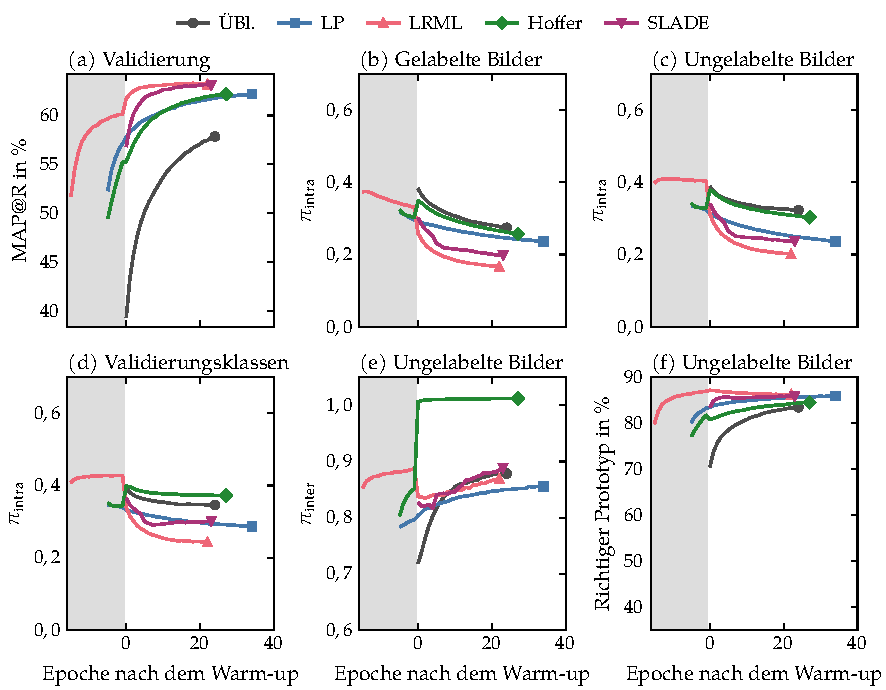
\includegraphics{neu/verlauf_k32}
  \caption[Trainingsverlauf bei 32 Labels je Klasse]{Validierungs-\acs{MAP@R} und Geometrie der Klassen über das Training bei $k=32$ (Cars196, Seed 2, Mittel über die fünf Verlustfunktionen und die vier Folds, ausgerichtet am Ende des Warm-ups). (a) Validierungs-\acs{MAP@R}, (b) bis (d) $\pi_{\mathrm{intra}}$ der gelabelten und der ungelabelten Bilder sowie der Validierungsklassen, (e) $\pi_{\mathrm{inter}}$, (f) Anteil der ungelabelten Bilder mit richtigem nächstem Klassenprototyp. Grau: Warm-up. Marker: Stopp des ersten Laufs.}
  \label{fig:a:verlauf32}
\end{figure}

\begin{figure}[tbp]
  \centering
  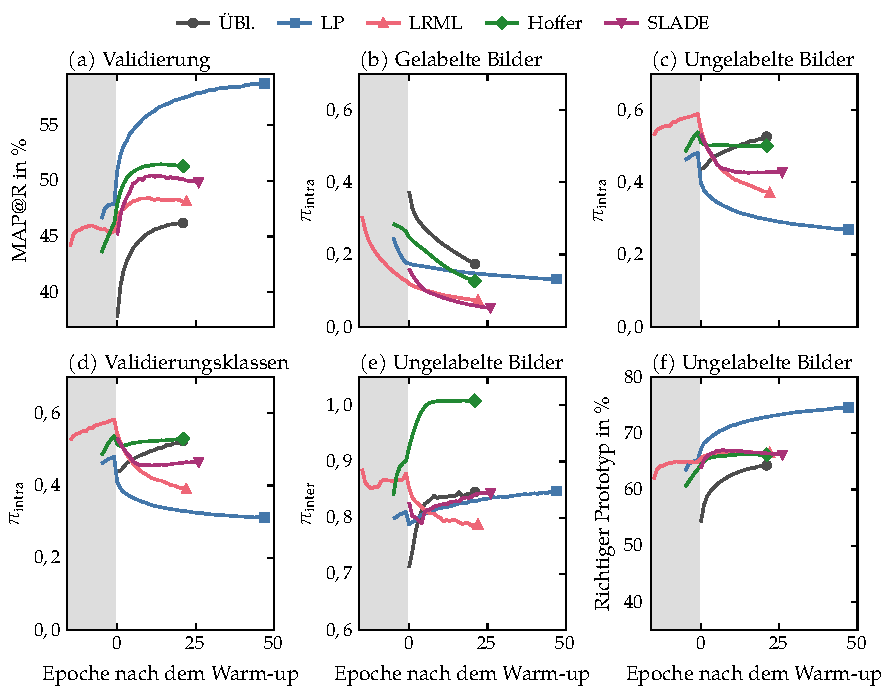
\includegraphics{neu/verlauf_k4}
  \caption[Trainingsverlauf bei vier Labels je Klasse]{Validierungs-\acs{MAP@R} und Geometrie der Klassen über das Training bei $k=4$, Teilabbildungen, Mittelung und Ausrichtung wie in Abbildung \ref{fig:a:verlauf32}.}
  \label{fig:a:verlauf4}
\end{figure}

\begin{figure}[tbp]
  \centering
  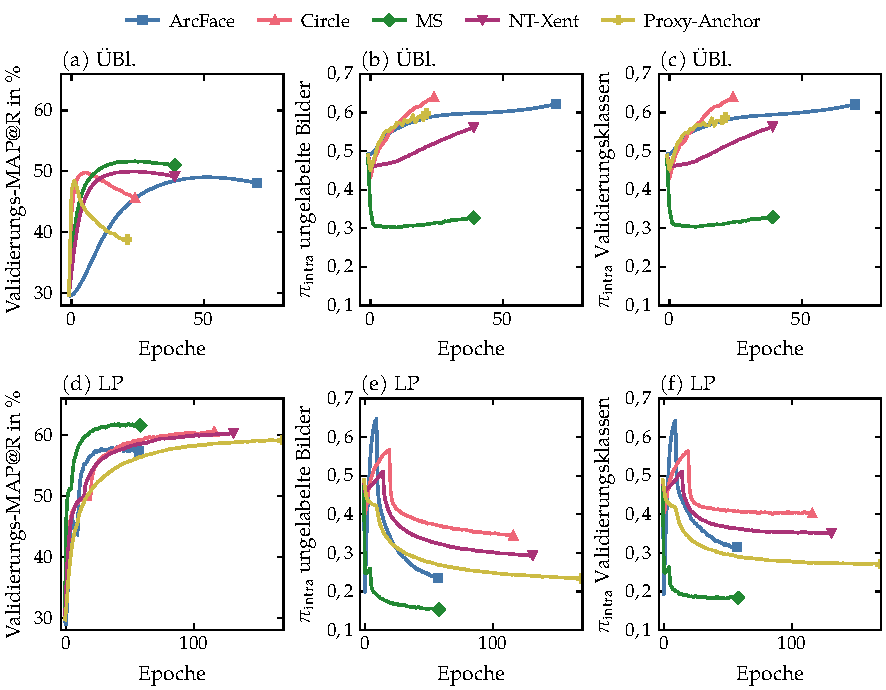
\includegraphics{neu/verlauf_verluste}
  \caption[Trainingsverlauf der \UEBL und von \acs{LP} mit allen Verlustfunktionen]{Validierungs-\acs{MAP@R} und $\pi_{\mathrm{intra}}$ der ungelabelten Bilder und der Validierungsklassen über das Training für die \UEBL (a bis c) und \acs{LP} (d bis f) bei $k=4$ mit allen fünf Verlustfunktionen (Cars196, Seed 2, Mittel über vier Folds, Marker am Kurvenende). Bei \acs{LP} mit ArcFace rückten bei Epoche 0 vorübergehend alle Bilder zusammen.}
  \label{fig:a:verluste}
\end{figure}

\begin{figure}[tbp]
  \centering
  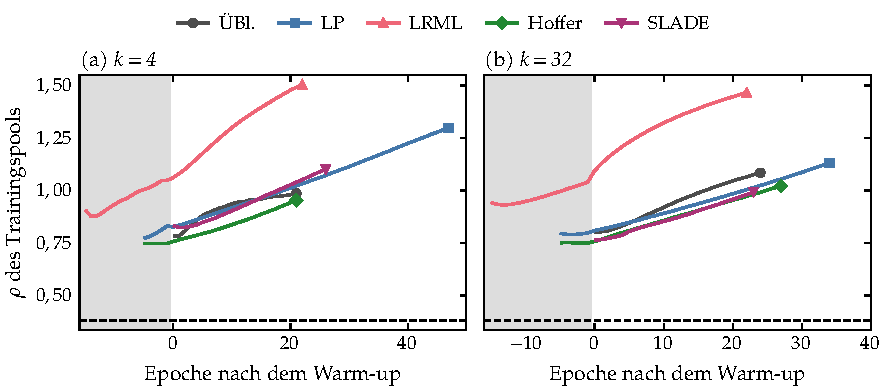
\includegraphics{neu/verlauf_rho}
  \caption[Spektraler Abfall über das Training]{Spektraler Abfall $\rho$ des Trainingspools über das Training bei (a) $k=4$ und (b) $k=32$ (Cars196, Seed 2, Mittel über die fünf Verlustfunktionen und die vier Folds, jeder Lauf am Ende seines Warm-ups ausgerichtet). Gestrichelt: DINOv2-Merkmale. Grau: Warm-up, gezeigt nur der allen Läufen gemeinsame Teil.}
  \label{fig:a:rho}
\end{figure}

\begin{figure}[tbp]
  \centering
  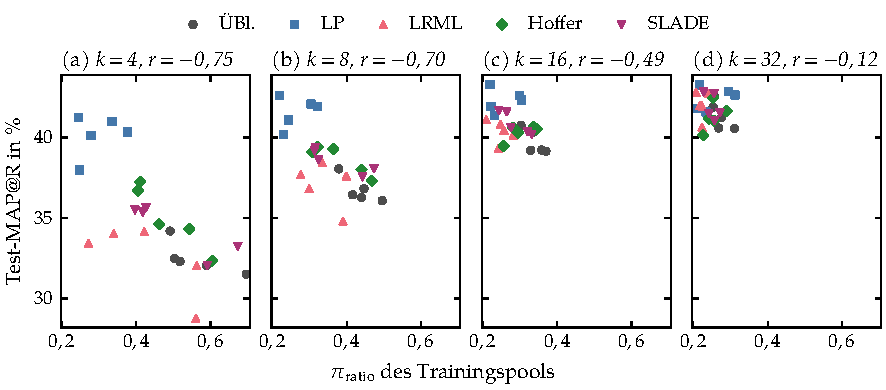
\includegraphics{neu/geometrie_korrelation}
  \caption[Geometrie und Retrieval-Leistung je Budget]{Test-\acs{MAP@R} der Einzelmodelle gegen $\pi_{\mathrm{ratio}}$ des Trainingspools nach dem Training für (a) $k=4$ bis (d) $k=32$, je Budget 25 Kombinationen aus Verfahren und Verlustfunktion (Cars196, Seed 2, Mittel über vier Folds). $r_{\mathrm{S}}$: Rangkorrelation nach Spearman innerhalb des Budgets.}
  \label{fig:e:geo:korrelation}
\end{figure}

\begin{table}[tbp]
\centering\small\setlength{\tabcolsep}{3.2pt}
\caption[Geometrie nach dem Training je Verlustfunktion]{$\pi_{\mathrm{intra}}$ der ungelabelten und, in Klammern, der gelabelten Bilder des Trainingspools und Test-MAP@R (Mean) nach dem Training je Verlustfunktion (Cars196, Seed 2, Mittel über vier Folds). Fett: kleinstes $\pi_{\mathrm{intra}}$ der ungelabelten Bilder und größte MAP@R je Zeile, bei gleichen gerundeten Werten nach dem ungerundeten Wert.}
\label{tab:a:geometrie}
\begin{tabular}{@{}l S[table-format=1.2] S[table-format=1.2] S[table-format=1.2] S[table-format=1.2] S[table-format=1.2] S[table-format=2.1] S[table-format=2.1] S[table-format=2.1] S[table-format=2.1] S[table-format=2.1]@{}}
\toprule
& \multicolumn{5}{c}{$\pi_{\mathrm{intra}}$ ungelabelt (gelabelt)} & \multicolumn{5}{c}{Test-MAP@R in \%} \\
\cmidrule(lr){2-6}\cmidrule(l){7-11}
{Verlust} & {\UEBL} & {LP} & {\acs{LRML}} & {Hoffer} & {SLADE} & {\UEBL} & {LP} & {\acs{LRML}} & {Hoffer} & {SLADE} \\
\midrule
\multicolumn{11}{@{}l}{\emph{$k=4$}} \\
ArcFace & 0.60 & \bfseries 0.26 & 0.57 & 0.56 & 0.60 & 32.1 & \bfseries 38.0 & 32.0 & 34.3 & 32.1 \\
 & {(0,16)} & {(0,07)} & {(0,08)} & {(0,16)} & {(0,05)} & & & & & \\
Circle & 0.52 & \bfseries 0.34 & 0.38 & 0.42 & 0.39 & 32.3 & \bfseries 41.0 & 34.1 & 36.7 & 35.7 \\
 & {(0,24)} & {(0,19)} & {(0,12)} & {(0,08)} & {(0,08)} & & & & & \\
MS & 0.31 & \bfseries 0.16 & 0.19 & 0.42 & 0.30 & 34.2 & \bfseries 41.3 & 33.4 & 37.3 & 35.5 \\
 & {(0,14)} & {(0,08)} & {(0,08)} & {(0,10)} & {(0,04)} & & & & & \\
NT-Xent & 0.51 & \bfseries 0.29 & 0.32 & 0.43 & 0.42 & 32.5 & \bfseries 40.1 & 34.0 & 34.6 & 35.4 \\
 & {(0,20)} & {(0,13)} & {(0,06)} & {(0,22)} & {(0,09)} & & & & & \\
Proxy-Anchor & 0.47 & \bfseries 0.23 & 0.27 & 0.62 & 0.40 & 31.5 & \bfseries 40.4 & 28.8 & 32.3 & 33.2 \\
 & {(0,11)} & {(0,12)} & {(0,03)} & {(0,20)} & {(0,10)} & & & & & \\
\addlinespace
\multicolumn{11}{@{}l}{\emph{$k=32$}} \\
ArcFace & 0.29 & \bfseries 0.21 & 0.25 & 0.32 & 0.30 & \bfseries 41.9 & 41.8 & 40.6 & 41.6 & 41.5 \\
 & {(0,20)} & {(0,21)} & {(0,18)} & {(0,25)} & {(0,23)} & & & & & \\
Circle & 0.35 & 0.31 & \bfseries 0.23 & 0.26 & 0.25 & 40.6 & 42.6 & 42.0 & 41.2 & \bfseries 42.7 \\
 & {(0,25)} & {(0,32)} & {(0,19)} & {(0,22)} & {(0,21)} & & & & & \\
MS & 0.21 & \bfseries 0.14 & 0.21 & 0.25 & 0.18 & 42.5 & \bfseries 43.3 & 42.7 & 40.1 & 42.8 \\
 & {(0,16)} & {(0,14)} & {(0,18)} & {(0,20)} & {(0,16)} & & & & & \\
NT-Xent & 0.30 & 0.23 & \bfseries 0.20 & 0.28 & 0.26 & 40.6 & 41.6 & \bfseries 42.8 & 41.1 & 41.5 \\
 & {(0,21)} & {(0,24)} & {(0,16)} & {(0,23)} & {(0,21)} & & & & & \\
Proxy-Anchor & 0.24 & 0.18 & \bfseries 0.18 & 0.29 & 0.22 & 41.2 & \bfseries 42.9 & 42.0 & 42.5 & 41.1 \\
 & {(0,17)} & {(0,19)} & {(0,13)} & {(0,20)} & {(0,17)} & & & & & \\
\bottomrule
\end{tabular}
\end{table}


\begin{table}[tbp]
\centering
\caption[Reinheit des $k$NN-Graphen von LRML]{Reinheit des $k$NN-Graphen von \acs{LRML} nach dem Training (Anteil der Kanten innerhalb einer Klasse in \%) mit der Nachbarzahl der Konfiguration der Geometrieläufe (Cars196, Seed~2, Mittel über vier Folds). Head ($-1$): vor dem ersten Optimierungsschritt. Nur innerhalb einer Zeile vergleichbar, weil sich die Nachbarzahlen unterscheiden.}
\label{tab:a:reinheit:lrml}
\begin{tabular}{@{}l S[table-format=2.0] S[table-format=2.1] S[table-format=2.1] S[table-format=2.1] S[table-format=2.1] S[table-format=2.1]@{}}
\toprule
{Verlust} & {Nachbarn} & {Head ($-1$)} & {$k=4$} & {$k=8$} & {$k=16$} & {$k=32$} \\
\midrule
ArcFace & 49 & 30.8 & 56.3 & 67.2 & 74.1 & 78.5 \\
Circle & 77 & 24.9 & 48.7 & 57.7 & 62.5 & 65.4 \\
\acs{MS} & 50 & 30.6 & 57.6 & 68.1 & 74.6 & 76.5 \\
NT-Xent & 52 & 30.1 & 58.1 & 68.1 & 73.7 & 76.6 \\
Proxy-Anchor & 25 & 39.4 & 62.1 & 74.5 & 82.2 & 85.2 \\
\bottomrule
\end{tabular}
\end{table}

\clearpage %
\begingroup\small\setstretch{1}\setlength{\tabcolsep}{4pt}
\begin{longtable}{@{}ll S[table-format=1.0] S[table-format=1.2] S[table-format=1.2] S[table-format=1.2] S[table-format=1.2] S[table-format=2.1] S[table-format=3.0] S[table-format=2.1]@{}}
\caption[Geometrie auf Semi-iNat-2021 und In-Shop für alle Budgets]{Geometrie nach dem Training für alle Budgets von Semi-iNat-2021, In-Shop und der In-Shop-Serie mit gelabelten Klassen (Seed 2, Mittel über die vier Folds und die Verlustfunktionen, die bei diesem Budget für alle Verfahren vollständig vorliegen, Anzahl: Zahl dieser Verlustfunktionen). $\pi^{\mathrm{U}}_{\mathrm{intra}}$: ungelabelte Bilder, $\pi^{\mathrm{V}}_{\mathrm{ratio}}$: Validierungsklassen, Prototyp: Anteil der ungelabelten Bilder mit richtigem nächstem Klassenprototyp in \%, übrige Spalten wie in Tabelle \ref{tab:e:geometrie}.}\label{tab:a:geometrie:weitere}\\
\toprule
{Budget} & {Modell} & {Anzahl} & {$\rho$} & {$\pi_{\mathrm{ratio}}$} & {$\pi^{\mathrm{U}}_{\mathrm{intra}}$} & {$\pi^{\mathrm{V}}_{\mathrm{ratio}}$} & {Prototyp} & {Epoche} & {MAP@R} \\
\midrule
\endfirsthead
\multicolumn{10}{@{}l}{\small Tabelle \thetable{} (Fortsetzung)}\\
\toprule
{Budget} & {Modell} & {Anzahl} & {$\rho$} & {$\pi_{\mathrm{ratio}}$} & {$\pi^{\mathrm{U}}_{\mathrm{intra}}$} & {$\pi^{\mathrm{V}}_{\mathrm{ratio}}$} & {Prototyp} & {Epoche} & {MAP@R} \\
\midrule
\endhead
\midrule
\multicolumn{10}{r@{}}{\emph{Fortsetzung auf der nächsten Seite}}\\
\endfoot
\bottomrule
\endlastfoot
\multicolumn{10}{@{}l}{\emph{Semi-iNat-2021}} \\
$k=2$ & \UEBL & 5 & 0.52 & 0.68 & 0.67 & 0.69 & 56.3 & 11 & 34.1 \\
 & LP &  & 0.60 & 0.62 & 0.58 & 0.66 & 62.0 & 31 & 34.6 \\
 & \acs{LRML} &  & 0.53 & 0.67 & 0.66 & 0.68 & 56.4 & 7 & 34.0 \\
 & Hoffer &  & 0.52 & 0.68 & 0.67 & 0.69 & 56.4 & 8 & 34.0 \\
 & SLADE &  & 0.52 & 0.69 & 0.66 & 0.70 & 56.4 & 11 & 34.0 \\
$k=4$ & \UEBL & 5 & 0.53 & 0.66 & 0.64 & 0.68 & 67.0 & 18 & 34.7 \\
 & LP &  & 0.60 & 0.61 & 0.56 & 0.66 & 71.0 & 39 & 35.3 \\
 & \acs{LRML} &  & 0.55 & 0.65 & 0.63 & 0.67 & 67.1 & 10 & 34.5 \\
 & Hoffer &  & 0.54 & 0.66 & 0.64 & 0.68 & 67.0 & 8 & 34.6 \\
 & SLADE &  & 0.53 & 0.65 & 0.63 & 0.68 & 67.1 & 15 & 34.6 \\
$k=16$ & \UEBL & 5 & 0.59 & 0.59 & 0.58 & 0.65 & 78.8 & 45 & 36.0 \\
 & LP &  & 0.64 & 0.57 & 0.53 & 0.65 & 79.6 & 57 & 36.4 \\
 & \acs{LRML} &  & 0.61 & 0.58 & 0.55 & 0.65 & 78.8 & 29 & 35.8 \\
 & Hoffer &  & 0.59 & 0.60 & 0.58 & 0.65 & 78.9 & 23 & 36.0 \\
 & SLADE &  & 0.58 & 0.57 & 0.57 & 0.63 & 78.9 & 50 & 36.0 \\
$k=100$ & \UEBL & 5 & 0.65 & 0.54 & 0.53 & 0.64 & 83.7 & 85 & 37.1 \\
 & LP &  & 0.64 & 0.57 & 0.52 & 0.65 & 81.7 & 59 & 36.2 \\
 & \acs{LRML} &  & 0.69 & 0.53 & 0.49 & 0.63 & 83.2 & 56 & 36.6 \\
 & Hoffer &  & 0.66 & 0.54 & 0.53 & 0.64 & 83.9 & 50 & 37.1 \\
 & SLADE &  & 0.65 & 0.51 & 0.51 & 0.59 & 83.2 & 104 & 36.8 \\
\addlinespace
\multicolumn{10}{@{}l}{\emph{In-Shop}} \\
$k=2$ & \UEBL & 5 & 1.28 & 0.32 & 0.31 & 0.36 & 71.9 & 203 & 54.8 \\
 & LP &  & 1.81 & 0.29 & 0.27 & 0.34 & 74.9 & 235 & 57.9 \\
 & \acs{LRML} &  & 2.04 & 0.27 & 0.20 & 0.32 & 73.4 & 133 & 56.4 \\
 & Hoffer &  & 2.09 & 0.27 & 0.31 & 0.32 & 74.1 & 152 & 57.9 \\
 & SLADE &  & 1.12 & 0.32 & 0.35 & 0.35 & 71.7 & 233 & 54.2 \\
$k=4$ & \UEBL & 5 & 1.73 & 0.23 & 0.26 & 0.28 & 76.9 & 396 & 59.3 \\
 & LP &  & 1.63 & 0.28 & 0.27 & 0.33 & 78.2 & 224 & 59.1 \\
 & \acs{LRML} &  & 2.01 & 0.23 & 0.20 & 0.27 & 76.8 & 146 & 58.9 \\
 & Hoffer &  & 2.26 & 0.24 & 0.28 & 0.28 & 75.2 & 180 & 59.1 \\
 & SLADE &  & 1.26 & 0.24 & 0.30 & 0.28 & 76.6 & 329 & 58.7 \\
\addlinespace
\multicolumn{10}{@{}l}{\emph{In-Shop-Serie mit gelabelten Klassen}} \\
\qty{5}{\percent} & \UEBL & 5 & 0.90 & 0.39 & 0.36 & 0.40 & {--} & 92 & 43.3 \\
 & LP &  & 1.28 & 0.37 & 0.25 & 0.38 & {--} & 43 & 41.8 \\
 & \acs{LRML} &  & 1.23 & 0.31 & 0.26 & 0.33 & {--} & 41 & 44.2 \\
 & Hoffer &  & 0.87 & 0.41 & 0.34 & 0.42 & {--} & 66 & 43.2 \\
 & SLADE &  & 0.86 & 0.42 & 0.26 & 0.44 & {--} & 75 & 43.4 \\
\qty{10}{\percent} & \UEBL & 5 & 1.03 & 0.36 & 0.35 & 0.38 & {--} & 168 & 48.1 \\
 & LP &  & 1.33 & 0.32 & 0.24 & 0.34 & {--} & 65 & 46.7 \\
 & \acs{LRML} &  & 1.44 & 0.26 & 0.24 & 0.28 & {--} & 78 & 49.2 \\
 & Hoffer &  & 1.00 & 0.39 & 0.33 & 0.41 & {--} & 130 & 47.9 \\
 & SLADE &  & 0.89 & 0.37 & 0.25 & 0.40 & {--} & 123 & 47.7 \\
\qty{25}{\percent} & \UEBL & 4 & 1.30 & 0.30 & 0.30 & 0.33 & {--} & 331 & 54.6 \\
 & LP &  & 1.37 & 0.27 & 0.19 & 0.29 & {--} & 112 & 51.0 \\
 & \acs{LRML} &  & 1.43 & 0.24 & 0.15 & 0.26 & {--} & 123 & 52.3 \\
 & Hoffer &  & 1.21 & 0.34 & 0.31 & 0.38 & {--} & 297 & 54.5 \\
 & SLADE &  & 0.95 & 0.30 & 0.22 & 0.32 & {--} & 161 & 52.2 \\
\qty{50}{\percent} & \UEBL & 3 & 1.48 & 0.26 & 0.30 & 0.30 & {--} & 306 & 57.8 \\
 & LP &  & 1.29 & 0.26 & 0.23 & 0.28 & {--} & 171 & 52.6 \\
 & \acs{LRML} &  & 1.66 & 0.22 & 0.16 & 0.25 & {--} & 298 & 56.2 \\
 & Hoffer &  & 1.32 & 0.27 & 0.31 & 0.31 & {--} & 353 & 58.0 \\
 & SLADE &  & 1.03 & 0.26 & 0.27 & 0.30 & {--} & 408 & 57.1 \\
\end{longtable}
\endgroup


\chapter{Verzögerte Patience}
\label{chap:anhang:verzoegerung}

Dieser Anhang ergänzt Abschnitt \ref{sec:training}. In manchen Folds brach die Validierungs-\ac{MAP@R} in der ersten Trainingsepoche stark ein, sodass ihr Höchstwert bereits vor dem Training lag. Derselbe Einbruch kann auch nach einem Warm-up auftreten. Anschließend stieg die Validierungs-\ac{MAP@R} zwar wieder an, aber so langsam, dass sie den Höchstwert nicht innerhalb der Patience übertraf und das Training abbrach. Als zu früh gilt ein Abbruch, wenn die beste Epoche vor der 20. Epoche nach dem Warm-up liegt (ohne Warm-up vor der 20. Trainingsepoche) und die Validierungs-\ac{MAP@R} bis zum Abbruch noch steigt. Als steigend gilt sie, wenn die Ausgleichsgerade durch ihre Werte der letzten zehn Epochen bis zum Abbruch eine positive Steigung hat. Mit verzögerter Patience verbrauchen die ersten 20 Epochen nach dem Warm-up, ohne Warm-up die ersten 20 Trainingsepochen, keine Patience. Danach zählt die Patience die Epochen, in denen die Validierungs-\ac{MAP@R} nicht über ihren höchsten Wert ab der letzten dieser Epochen steigt. Gewählt wird wie ohne Verzögerung das Modell der Epoche mit der besten Validierungs-\ac{MAP@R}.

Zu früh beendet wurden 541 Folds in 339 Läufen aus beiden Phasen, dem Versuch mit externen Bildern und den Geometrieläufen. Ausgenommen sind die Läufe auf \ac{CUB} mit ihrer Patience von 40 Epochen und die Versuche der Hyperparametersuche. Die Ablationen bei $k=8$ wurden für jeden Lauf mit Verzögerung trainiert (Abschnitt \ref{sec:m:phase2}).

Für die 321 Läufe mit einem zu früh beendeten Fold, für die die Arbeit die Variante ohne Verzögerung berichtet, zeigen Abbildung \ref{fig:a:verzoegerung} und Tabelle \ref{tab:anhang:verzoegerung} die Test-\ac{MAP@R} mit verzögerter Patience als zweiten Wert. Im Mittel änderte sie sich um \num{0.06} Prozentpunkte. Bis zum früheren Abbruch durchliefen beide Varianten in 313 Läufen dieselbe Validierungskurve. In 188 Läufen validierten sie gleich und wählten dieselbe Epoche, in 132 validierte die Variante mit Verzögerung besser. Die Differenz in der Validierung hängt mit der im Test zusammen (Korrelation \num{0.73}), sagt sie aber nur grob voraus. In 70 der 132 Läufe sank die Test-\ac{MAP@R}, vor allem mit externen Bildern auf Cars196. Dort validierte die Variante mit Verzögerung in 64 der 133 Läufe besser, die Test-\ac{MAP@R} sank aber in 58 davon, im Mittel um \num{0.8} Prozentpunkte. Die Validierung überschätzt dort also den Nutzen eines längeren Trainings. Am stärksten stieg die Test-\ac{MAP@R} in den Ablationen der Phase 2, um bis zu \num{7.2} Prozentpunkte bei \ac{LP} mit ArcFace und der Konfidenzschwelle \num{0.7} auf In-Shop. In den beiden Läufen mit den größten Einbrüchen der Sweeps von \ac{SLADE} (Abschnitt \ref{sec:e:sweeps}) beendete die Patience das Training in mehreren Folds zu früh. Mit verzögerter Patience verlor \ac{SLADE} beim kleinen Basis-Zielverhältnis \num{11.5} statt \num{16.6} und bei 512 ungelabelten Bildern je Batch \num{14.9} statt \num{20.5} Prozentpunkte.

Für die \UEBL mit Proxy-Anchor in der In-Shop-Serie mit gelabelten Klassen bei 10 bis \qty{50}{\percent} berichtet die Arbeit die Variante mit Verzögerung, in 15 Läufen und den drei zugehörigen Geometrieläufen. Ohne Verzögerung übertraf die Validierungs-\ac{MAP@R} dort in mindestens einem Fold innerhalb der Patience nie den Wert vor dem ersten Trainingsschritt. Ihre Test-\ac{MAP@R} läge dann bei \qty{13.3}{\percent} bis \qty{39.7}{\percent} statt \qty{48.0}{\percent} bis \qty{57.4}{\percent}, weil einzelne Folds den zufällig initialisierten Head wählten.

\begin{figure}[tbp]
  \centering
  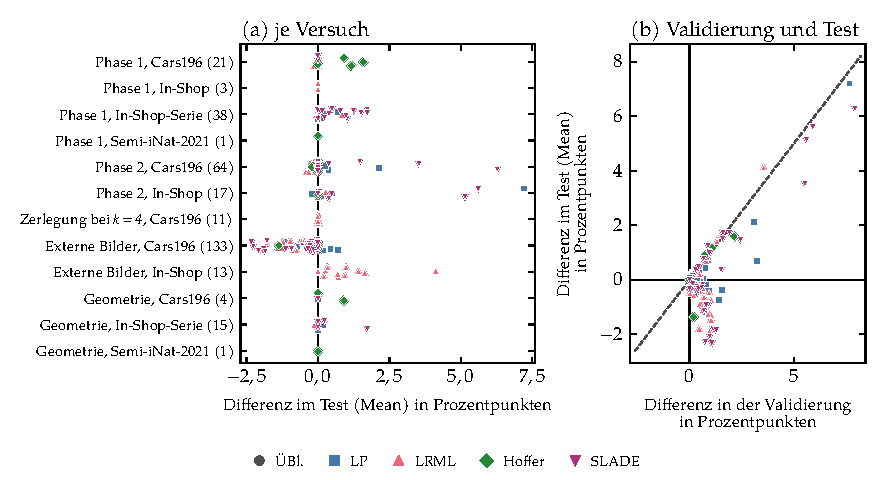
\includegraphics{neu/verzoegerung}
  \caption[Wirkung der verzögerten Patience je Lauf]{Test-\acs{MAP@R} der Einzelmodelle mit verzögerter Patience minus der ohne Verzögerung für die 321 Läufe mit einem zu früh beendeten Fold, (a) je Versuch mit der Zahl der Läufe, (b) gegen die Differenz der Validierungs-\acs{MAP@R}. Gestrichelt: gleiche Differenz in Validierung und Test. Ohne die 18 Läufe der \UEBL mit Proxy-Anchor in der In-Shop-Serie.}
  \label{fig:a:verzoegerung}
\end{figure}

\begin{table}[tbp]
\centering
\caption[Wirkung der verzögerten Patience]{Läufe mit einem zu früh beendeten Fold (Abschnitt \ref{sec:training}): Test-MAP@R mit verzögerter Patience minus der ohne Verzögerung in Prozentpunkten, Mittel und Spanne über die Läufe sowie die Zahl der Läufe, die mit Verzögerung besser validierten.}
\label{tab:anhang:verzoegerung}
\small
\begin{tabular}{@{}l S[table-format=3.0] S[table-format=-1.2] c S[table-format=-1.2] S[table-format=3.0]@{}}
\toprule
{Versuch} & {Läufe} & {Mean} & {\shortstack{Spanne\\(Mean)}} & {Concat} & {\shortstack{Validierung\\besser}} \\
\midrule
Phase 1, Cars196 & 21 & 0.17 & \num{-0.1} bis \num{1.6} & 0.12 & 4 \\
Phase 1, In-Shop & 3 & 0.00 & \num{0.0} bis \num{0.0} & 0.00 & 0 \\
Phase 1, In-Shop-Serie & 38 & 0.32 & \num{-0.1} bis \num{1.7} & 0.46 & 17 \\
Phase 1, Semi-iNat-2021 & 1 & 0.00 & \num{0.0} bis \num{0.0} & 0.00 & 0 \\
Phase 2, Cars196 & 64 & 0.20 & \num{-0.4} bis \num{6.3} & 0.23 & 16 \\
Phase 2, In-Shop & 17 & 1.15 & \num{-0.2} bis \num{7.2} & 1.61 & 11 \\
Zerlegung bei $k=4$, Cars196 & 11 & 0.01 & \num{0.0} bis \num{0.1} & 0.10 & 2 \\
Externe Bilder, Cars196 & 133 & -0.33 & \num{-2.3} bis \num{0.7} & 0.06 & 64 \\
Externe Bilder, In-Shop & 13 & 0.89 & \num{0.0} bis \num{4.1} & 0.86 & 11 \\
Geometrie, Cars196 & 4 & 0.23 & \num{0.0} bis \num{0.9} & 0.12 & 1 \\
Geometrie, In-Shop-Serie & 15 & 0.15 & \num{-0.1} bis \num{1.7} & 0.25 & 6 \\
Geometrie, Semi-iNat-2021 & 1 & 0.00 & \num{0.0} bis \num{0.0} & 0.00 & 0 \\
\midrule
alle & 321 & 0.06 & \num{-2.3} bis \num{7.2} & 0.27 & 132 \\
\bottomrule
\end{tabular}
\end{table}



% die Thesen
\pagestyle{empty}	
\addchap{Thesen}
\begin{enumerate}
  \item Ungelabelte Bilder können Deep Metric Learning auf eingefrorenen DINOv2-Merkmalen verbessern, wenn wenige Labels vorliegen, zusätzliche echte Labels die supervised Referenz noch deutlich verbessern und die ungelabelten Bilder aus den gelabelten Klassen stammen. Bei den Budgets der Hyperparametersuche gewinnt Label Propagation auf Cars196 und In-Shop in jedem gepaarten Vergleich, um 2,2 bzw. 3,2 Prozentpunkte. Mit der übertragenen Konfiguration erreicht sie auf Cars196 mit vier gelabelten Trainingsbildern je Klasse die Referenz mit sechzehn.
  \item Der Nutzen ungelabelter Bilder sinkt mit dem Label-Budget. Bei 32 gelabelten Bildern je Klasse (Cars196) liegt er im Mittel unter einem Prozentpunkt, bei 60\,\% gelabeltem Pool (In-Shop) ist er verschwunden.
  \item Sind die vortrainierten Merkmale bereits nahe am Erreichbaren, wie auf \ac{CUB}, bleibt selbst ein supervised trainierter Head mit wenigen Labels als Einzelmodell unter den unveränderten Merkmalen. Ungelabelte Bilder bringen dort gegenüber der supervised Referenz nur kleine Gewinne, vor allem im Ensemble.
  \item Die für die semi-supervised Verfahren anders gewählten Hyperparameter erklären die Gewinne nicht. Dass die ungelabelten Bilder auch mit den Hyperparametern der supervised Referenz helfen, gilt aber vor allem für Label Propagation. Je nach Verfahren und Verlustfunktion hebt schon der semi-supervised Term auf den gelabelten Bildern allein die Leistung, bei der Laplace-Regularisierung auf Cars196 mit allen fünf Verlustfunktionen und bei Hoffer auf In-Shop mit vier.
  \item Label Propagation und Laplace-Regularisierung wirken über die aus den Daten berechnete Nachbarschaft, denn ein zufällig umverdrahteter Graph schadet stark.
  \item Für Pseudo-Labels im Metric Learning ist die Fehlerrate allein kein ausreichendes Maß. Wie stark falsche Labels schaden, hängt auch von der Verlustfunktion und von den betroffenen Bildern ab. Mit einem Seed liegt Label Propagation auf Cars196 mit drei der fünf und auf In-Shop mit allen fünf Verlustfunktionen über Läufen mit zufälligen Fehlern gleicher mittlerer Häufigkeit.
  \item Ob ein Verfahren als besser gilt, hängt davon ab, ob ein Einzelmodell oder ein Ensemble der Fold-Modelle bewertet wird. Beide Sichtweisen müssen deshalb getrennt berichtet werden.
  \item Stammen die ungelabelten Bilder aus Klassen ohne Labels, schadet Label Propagation in der hier verwendeten Form, die stets einen Teil der Bilder übernimmt. Die Laplace-Regularisierung hilft bei wenigen gelabelten Klassen im Ensemble weiter, als Einzelmodell aber nur mit Circle.
\end{enumerate}


\end{document}

% Ende der Datei
